% \NeedsTeXFormat{LaTeX2e}
% \documentclass[12pt,a4paper,oneside,openright]{Book}
\documentclass[11pt,a4paper]{report}
\pdfcompresslevel=9
\pdfobjcompresslevel=2
%\pagestyle{empty}
\usepackage[utf8]{vietnam}
\usepackage{array}
% \usepackage[titletoc]{appendix}
\usepackage{listings}
\usepackage{indentfirst}
\usepackage{amsmath,amsfonts,amssymb,fancyhdr}
\usepackage{amsthm,amsxtra,latexsym, amscd}
\usepackage[bottom=2cm, left=3cm,right=2cm,top=2cm] {geometry}
\usepackage[unicode]{hyperref}
\usepackage{graphicx}
\usepackage{algorithmic}
\usepackage{algorithm}
\usepackage{fancyhdr,graphicx,amsmath,amssymb}
\graphicspath{images}
\usepackage{titlesec}
\usepackage{color}
\usepackage[table]{xcolor}
\graphicspath{ {images}}
\setcounter{secnumdepth}{6}
\usepackage{afterpage}
\usepackage{boxedminipage,fancybox}
\usepackage{subcaption}
\usepackage{float}
\usepackage{xcolor,soul}
\sethlcolor{lightgray}
\usepackage{enumerate}
\usepackage[shortlabels]{enumitem}
% \usepackage[automake]{glossaries}
\usepackage{xcolor}
\usepackage{tabularray}
% \makeglossaries
\usepackage{rotating}
\usepackage{tikz}
\usetikzlibrary{trees,shapes.geometric,arrows.meta,positioning,fit,backgrounds,calc}
\usepackage{pgfplots}
\pgfplotsset{compat=1.18}
\usepackage{forest}
\usepackage{booktabs}
\usepackage{graphicx}
\usepackage{pdfpages}
\usepackage{pmboxdraw}
\usepackage{datetime}
% \usepackage{csquotes}

\usepackage[
backend=biber,
style=ieee,
sorting=none
]{biblatex}

\addbibresource{ref.bib}
% \font\tench=t5-lmb10 at18pt%

% \titleformat{\chapter}[display]
% {\normalfont\large\filcenter\bfseries}
% {{{\chaptertitlename\,}\thechapter}} {1pc}{
% {\tench}\MakeUppercase}



% \usepackage{minitoc}
\usepackage{lipsum} % just to generate text for the example
%------------------------------------------------------------
%   CHAPTER CUSTOM
%------------------------------------------------------------
\titleformat{\chapter}[display]
{\bfseries\Large}
{\filright\MakeUppercase{\chaptertitlename} \Huge\thechapter}
{1ex}
{\titlerule\vspace{1ex}\filleft}
[\vspace{1ex}\titlerule]
%------------------------------------------------------------
%   CHAPTER CUSTOM
%------------------------------------------------------------
%------------------------------------------------------------
%   CUSTOM SIZE SECTION
%------------------------------------------------------------
\titleformat*{\section}{\LARGE\bfseries}
\titleformat*{\subsection}{\Large\bfseries}
\titleformat*{\subsubsection}{\large\bfseries}
\titleformat*{\paragraph}{\large\bfseries}
\titleformat*{\subparagraph}
{\large\bfseries}
\titleformat{\paragraph}[block]{\normalfont\normalsize\bfseries}{\theparagraph}{1em}{}


\renewcommand{\theequation}{\thechapter.\arabic{equation}}% Danh lai so cong thuc toan
% \font\tieude=t5-lmb10 at 14pt
%------------------------------------------------------------
\theoremstyle{definition}
\theoremstyle{plain}
\newtheorem{theorem}{Định lý}[section]
\newtheorem{dl}[theorem]{Định lý}
\newtheorem{hq}[theorem]{Hệ quđả}
\newtheorem{corollary}[theorem]{Hệ quả}
\newtheorem{problem}{Bài toán}
\newtheorem{main}{Định lý cơ bản}
\newtheorem{bd}[theorem]{Bổ đề}
\newtheorem{lemma}[theorem]{Bổ đề}
\newtheorem{md}[theorem]{Mệnh đề}
\newtheorem{proposition}[theorem]{Mệnh đề}
\theoremstyle{definition}
\newtheorem{dn}[theorem]{Định nghĩa}
\newtheorem{definition}[theorem]{Định nghĩa}
\theoremstyle{definition}
\theoremstyle{remark}
\theoremstyle{definition}
\newtheorem{note}[theorem]{\bf Chú ý}
\newtheorem{vd}[theorem]{\bf Ví dụ}
\newtheorem{example}[theorem]{Ví dụ}
\newtheorem{nx}[theorem]{\bf Nhận xét}
\newtheorem{remark}[theorem]{Nhận xét}
\newtheoremstyle{vd}% name
  {3pt}%      Space above
  {3pt}%      Space below
  {}%         Body font
  {}%         Indent amount (empty = no indent, \parindent = para indent)
  {\bfseries}% Thm head font
  {.}%        Punctuation after thm head
  {.5em}%     Space after thm head: " " = normal interword space;
        %       \newline = linebreak
  {}%

\usepackage{verbatimbox}
%------------------------------------------------------------
%   CUSTOM HEADER AND FOOTER
%------------------------------------------------------------
\pagestyle{fancy}
\fancyhf{}
\fancyhead[C]{\thepage}
\fancyhead[R]{%
\begin{minipage}[b]{0.40\textwidth}
\raggedleft\nouppercase{\rightmark}
\end{minipage}
}
\renewcommand{\headrulewidth}{0.3pt}
\renewcommand{\footrulewidth}{0pt}
\setlength{\headheight}{30pt}
\setlength{\headsep}{10pt}

\fancypagestyle{plain}{
  \fancyhf{}
  \fancyhead[C]{\thepage}
  \renewcommand{\headrulewidth}{0pt}
  \renewcommand{\footrulewidth}{0pt}
}

% ---------------------------------------------------------------
% --------------------- CUSTOM TBLR SECTION ---------------------
\DefTblrTemplate{contfoot-text}{default}{Tiếp tục ở trang sau}
\DefTblrTemplate{conthead-text}{default}{(Tiếp theo)}
% ---------------------------------------------------------------

\usepackage{titletoc}% http://ctan.org/pkg/titletoc
\titlecontents*{chapter}% <section-type>
  [0pt]% <left>
  {}% <above-code>
  {\bfseries\chaptername\ \thecontentslabel\quad}% <numbered-entry-format>
  {}% <numberless-entry-format>
  {\bfseries\hfill\contentspage}% <filler-page-format>

% \flushbottom

\raggedbottom

\begin{document}
% \setlength{\parindent}{1.5fem}
\renewcommand{\baselinestretch}{1.5}

\renewcommand{\appendixname}{Appendix}
\renewcommand{\figurename}{Hình}
\renewcommand{\tablename}{Bảng}
\renewcommand{\contentsname}{Mục lục}

\renewcommand{\listfigurename}{Danh sách hình ảnh}
\renewcommand{\listtablename}{Danh sách bảng}
\renewcommand{\refname}{Tài liệu tham khảo}

% \font\chuong=t5-lmb10 at12pt%
% \def\chaptername{\chuong CHƯƠNG}
\fontsize{12pt}{12pt}\selectfont
\def\e{$\varepsilon$}
\def\ptd {\,$p$-trơn đều\,}
\def\xs{$(\Omega,\mathcal{F},\mathbf{P})$}
\def\F{$\mathcal{F}$}
\def\X{$\Bbb{E}$\,\,}
\def\a{$\mathcal{A}$}
\def\E{\,$\Bbb{E}$\,}
\def\be{$\mathcal{B}(\Bbb{E})$\,\,}
\def\spm{$E,;\;{\mathcal{B}}$}
\def\htxs{\xrightarrow{\mathbf{P}}}
\def\m{{\bf m}}
\def\n{{\bf n}}
\def\k{{\bf k}}
\def\l{{\bf l}}
%----------------------------------------------------------------------------
\def\RR{$\Bbb{R}\times\Bbb{R}$}
\def\R2{$\Bbb{R}^2$}
\def\Fn{\mathcal{F}_n}
\def\Fmn{\mathcal{F}_{mn}}
\def\Fij{\mathcal{F}_{ij}}
\def\Xi{\{X_i, i\geq 1\}}
\def\Xij{\{X_{ij};i\geq 1,j\geq 1\}}
%--------------------------------------------------------------------------
\newcommand{\I}{\mathbb I}% hàm chỉ tiêu
\newcommand{\bE}{\mathbb E}% không gian Banach
\newcommand{\fP}{\mathbf P}% xác suất
\newcommand{\mL}{\mathcal{L}}
\newcommand{\mF}{\mathcal{F}\,}
\newcommand{\fE}{\mathbf E}
\newcommand{\BE}{$\mathcal{B}(\mathbb{E})$\,}
\newcommand{\hcc}{$\xrightarrow{h.c.c}$\,}
\newcommand{\tb}{$\xrightarrow{\mathcal{L}}$}
\newcommand{\xij}{$\{X_{ij}; i, j \geq1\}$\,}
\newcommand{\xmn}{$\{X_{mn}; m\geq 1, n \geq1\}$\,}
\newcommand{\aij}{$\{A_{mnij};\, m, n, i, j \geq  1\}$}
%-----------------------------------------------------------------------
\def\al{{\alpha}}
\def\R{{\Bbb R}}
\def\F{{\mathcal F}}
\def\N{\Bbb{N}^d}
%----------------------------------------------------------------------------------------------------------%

%New colors defined below
\definecolor{codegreen}{rgb}{0,0.6,0}
\definecolor{codegray}{rgb}{0.5,0.5,0.5}
\definecolor{codepurple}{rgb}{0.58,0,0.82}
\definecolor{backcolour}{rgb}{0.95,0.95,0.92}
\definecolor{MintGreen}{rgb}{0.603,0.996,0.721}
\definecolor{Onahau}{rgb}{0.8,0.976,1}
\definecolor{bashbg}{RGB}{245,248,250}
\definecolor{bashprompt}{RGB}{0,102,204}
\definecolor{bashcomment}{RGB}{56,142,60}
\definecolor{bashstring}{RGB}{173,20,87}
\definecolor{bashoption}{RGB}{230,81,0}

%Code listing style named "mystyle"
\lstdefinestyle{mystyle}{
  backgroundcolor=\color{backcolour},   commentstyle=\color{codegreen},
  keywordstyle=\color{magenta},
  numberstyle=\tiny\color{codegray},
  stringstyle=\color{codepurple},
  basicstyle=\ttfamily\footnotesize,
  breakatwhitespace=false,         
  breaklines=true,                 
  captionpos=b,                    
  keepspaces=true,                 
  numbers=left,                    
  numbersep=5pt,                  
  showspaces=false,                
  showstringspaces=false,
  showtabs=false,                  
  tabsize=2
}

\lstdefinestyle{inlinecode}{
  basicstyle=\ttfamily\normalsize,
  backgroundcolor=\color{backcolour},
  keywordstyle=\color{magenta},
  commentstyle=\color{codegreen},
  stringstyle=\color{codepurple},
  showspaces=false,
  showstringspaces=false,
  keepspaces=true,
  breaklines=false
}

%"mystyle" code listing set
\lstset{style=mystyle}

\colorlet{punct}{blue!70!black}
\definecolor{background}{RGB}{245,248,250}
\definecolor{delim}{RGB}{30,64,175}
\colorlet{numb}{teal!70!black}

\lstdefinelanguage{json}{
    basicstyle=\normalfont\ttfamily,
    numbers=left,
    numberstyle=\scriptsize,
    stepnumber=1,
    numbersep=8pt,
    showstringspaces=false,
    breaklines=true,
    frame=lines,
    backgroundcolor=\color{background},
    literate=
     *{0}{{{\color{numb}0}}}{1}
      {1}{{{\color{numb}1}}}{1}
      {2}{{{\color{numb}2}}}{1}
      {3}{{{\color{numb}3}}}{1}
      {4}{{{\color{numb}4}}}{1}
      {5}{{{\color{numb}5}}}{1}
      {6}{{{\color{numb}6}}}{1}
      {7}{{{\color{numb}7}}}{1}
      {8}{{{\color{numb}8}}}{1}
      {9}{{{\color{numb}9}}}{1}
      {:}{{{\color{punct}{:}}}}{1}
      {,}{{{\color{punct}{,}}}}{1}
}

\lstdefinelanguage{yaml}{
  keywords={true,false,null,y,n,yes,no,on,off},
  keywordstyle=\color{blue}\bfseries,
  basicstyle=\ttfamily\footnotesize,
  sensitive=false,
  comment=[l]{\#},
  commentstyle=\color{codegreen},
  stringstyle=\color{codepurple},
  morestring=[b]',
  morestring=[b]",
  showstringspaces=false,
  breaklines=true,
  breakatwhitespace=false,
  tabsize=2
}

\lstdefinelanguage{bash}{
  sensitive=true,
  alsoletter={-},
  morekeywords={sudo,apt,apt-get,install,update,upgrade,ros2,colcon,source,cd,ls,cat,echo,export,launch,run,mkdir,rm,cp,mv},
  morekeywords=[2]{-y,--symlink-install,--help},
  keywordstyle=\color{bashprompt}\bfseries,
  keywordstyle=[2]\color{bashoption}\bfseries,
  comment=[l]{\#},
  commentstyle=\color{bashcomment}\itshape,
  morestring=[b]",
  morestring=[b]',
  stringstyle=\color{bashstring}
}

\lstdefinestyle{bashstyle}{
  language=bash,
  backgroundcolor=\color{bashbg},
  basicstyle=\ttfamily\footnotesize,
  frame=single,
  rulecolor=\color{codegray},
  numbers=left,
  numberstyle=\tiny\color{codegray},
  numbersep=6pt,
  showstringspaces=false,
  breaklines=true,
  breakatwhitespace=true,
  keepspaces=true,
  tabsize=2
}

\lstdefinestyle{DOS}        %terminal command style
{
    backgroundcolor=\color{black},
    basicstyle=\scriptsize\color{white}\ttfamily
}
\lstdefinestyle{csharp} {
    language=[Sharp]C, 
    frame=lr, 
    rulecolor=\color{blue!80!black}
}

%----------------------------------------------------------------------------------------------------------%
\newcommand{\td}{\fontfamily{ptm}\selectfont}
\setlength{\fboxsep} {1pt}
\begin{titlepage}
\thispagestyle{empty}


\begin{tikzpicture}[remember picture, overlay]
\draw [line width=1pt]
    ($ (current page.north west) + (2.5cm,-2.0cm) $)
    rectangle
    ($ (current page.south east) + (-1.5cm,1.5cm) $);
\draw [line width=3pt]
    ($ (current page.north west) + (2.65cm,-2.15cm) $)
    rectangle
    ($ (current page.south east) + (-1.65cm,1.65cm) $); 
\end{tikzpicture}

\begin{center}
    {\td\fontsize{12pt}{14pt}\selectfont ĐẠI HỌC QUỐC GIA THÀNH PHỐ HỒ CHÍ MINH}\\
    {\td\bfseries\fontsize{13pt}{15pt}\selectfont TRƯỜNG ĐẠI HỌC BÁCH KHOA}\\
    \rule{7cm}{0.4pt}
\end{center}

% \vspace{0.6cm}
% \begin{center}
% 
\includegraphics[width=4cm,height=4cm]{Images/Logo BK.png}\\
% \end{center}

\vspace{1.5cm}
\begin{center}
 {\td\bfseries\fontsize{16pt}{18pt}\selectfont TRẦN NGỌC CÁT}
\end{center}
\vspace{0.5cm}

\begin{center}
    {\td\bfseries\fontsize{20pt}{24pt}\selectfont NGHIÊN CỨU VÀ PHÁT TRIỂN}\\[0.1cm]
    {\td\bfseries\fontsize{20pt}{24pt}\selectfont HỆ THỐNG ĐIỀU KHIỂN CÁNH TAY ROBOT VỚI ROS2}\\[0.1cm]
    {\td\bfseries\fontsize{20pt}{24pt}\selectfont ĐỒNG BỘ KÍNH THỰC TẾ ẢO (VR)}\\[0.25cm]
    % \centerline{\bf \td \Large TÍCH HỢP AI XỬ LÝ TẠI BIÊN}
    \vspace{.5cm}
    {\td\bfseries\fontsize{20pt}{24pt}\selectfont \uppercase{Research and Development of}}\\[0.1cm]
    {\td\bfseries\fontsize{20pt}{24pt}\selectfont \uppercase{a Robotic Arm Control System Using ROS2}}\\[0.1cm]
    {\td\bfseries\fontsize{20pt}{24pt}\selectfont \uppercase{with Virtual Reality (VR) Headset Synchronization}}\\[0.25cm]
    \vspace{.1cm}
    {\td\fontsize{13pt}{15pt}\selectfont Chuyên ngành: Khoa học máy tính}\\[0.1cm]
    \vspace{.1cm}
    {\td\fontsize{13pt}{15pt}\selectfont Mã ngành: 8480101}
\end{center}

\vspace{1cm}

\begin{center}
    {\td\bfseries\fontsize{20pt}{24pt}\selectfont ĐỀ ÁN TỐT NGHIỆP}\\[0.1cm]
\end{center}


\vspace{0.3cm}

\vfill
\begin{center}
{\td\fontsize{13pt}{15pt}\selectfont Thành phố Hồ Chí Minh, tháng \number\month\ năm \number\year}
\end{center}
\end{titlepage}
 
\newpage
\thispagestyle{empty}


\begin{tikzpicture}[remember picture, overlay]
\draw [line width=1pt]
    ($ (current page.north west) + (2.5cm,-2.0cm) $)
    rectangle
    ($ (current page.south east) + (-1.5cm,1.5cm) $);
\end{tikzpicture}

\vspace*{0.1cm}

\begin{center}
    {\td\fontsize{13pt}{15pt}\selectfont CÔNG TRÌNH ĐƯỢC HOÀN THÀNH TẠI}\\[0.1cm]
    {\td\fontsize{13pt}{15pt}\selectfont TRƯỜNG ĐẠI HỌC BÁCH KHOA -- ĐHQG-HCM}
\end{center}

\vspace{0.6cm}

\noindent{\td\fontsize{13pt}{15pt}\selectfont
    Cán bộ hướng dẫn khoa học: TS. Lê Trọng Nhân
    \begin{center}
        (Ghi rõ họ, tên, học hàm, học vị và chữ ký)
    \end{center}
    Cán bộ chấm nhận xét 1: PGS.TS Lê Kim Hùng
    \begin{center}
        (Ghi rõ họ, tên, học hàm, học vị và chữ ký)
    \end{center}
    Cán bộ chấm nhận xét 2:
    \begin{center}
        (Ghi rõ họ, tên, học hàm, học vị và chữ ký)
    \end{center}
    \vspace{0.3cm}
    Đề án tốt nghiệp được bảo vệ tại Trường Đại học Bách Khoa -- ĐHQG-HCM ngày 19 tháng 06 năm 2026.\\[0.35cm]
}

\noindent{\td\fontsize{13pt}{15pt}\selectfont
Thành phần Hội đồng đánh giá Đề án tốt nghiệp gồm:\\[0.1cm]
(Ghi rõ họ, tên, học hàm, học vị của Hội đồng chấm bảo vệ Đề án tốt nghiệp)
}

\begin{flushleft}
{\td\fontsize{13pt}{15pt}\selectfont
    1. TS. Võ Tuấn Bình \\[0.2cm]
    2. TS. Phan Trần Minh Khuê \\[0.2cm]
    3. PGS.TS. Lê Kim Hùng \\[0.2cm]
    4. \\[0.2cm]
    5.
}
\end{flushleft}

\vspace{0.35cm}

\begin{center}
    {\td\fontsize{13pt}{15pt}\selectfont Xác nhận của Chủ tịch Hội đồng đánh giá Đề án tốt nghiệp và Trưởng khoa quản lý ngành sau khi đề án đã được sửa chữa (nếu có).}
\end{center}

\vspace{0.35cm}

\noindent\makebox[\textwidth][c]{%
\begin{tabular}{c@{\hspace{2cm}}c}
{\td\bfseries\fontsize{13pt}{15pt}\selectfont CHỦ TỊCH HỘI ĐỒNG} &
{\td\bfseries\fontsize{13pt}{15pt}\selectfont TRƯỞNG KHOA} \
\end{tabular}%
}

\newpage
\addcontentsline{toc}{chapter}{NHIỆM VỤ ĐỀ ÁN TỐT NGHIỆP}
\vspace{0.2cm}

\noindent
\begin{minipage}[t]{0.45\textwidth}
    \centering
    {\fontsize{11pt}{11pt}\selectfont ĐẠI HỌC QUỐC GIA TP. HỒ CHÍ MINH}\\
    {\fontsize{11pt}{11pt}\selectfont \textbf{TRƯỜNG ĐẠI HỌC BÁCH KHOA}}
    \vspace{0.05cm}
    \noindent\makebox[\linewidth][c]{\rule{0.65\linewidth}{0.4pt}}
\end{minipage}%
\begin{minipage}[t]{0.55\textwidth}
    \centering
    {\fontsize{9pt}{9pt}\selectfont \textbf{CỘNG HÒA XÃ HỘI CHỦ NGHĨA VIỆT NAM}}\\
    {\fontsize{11pt}{11pt}\selectfont \textbf{Độc lập - Tự do - Hạnh phúc}}
    \vspace{0.05cm}
    \noindent\makebox[\linewidth][c]{\rule{0.65\linewidth}{0.4pt}}
\end{minipage}



\vspace{0.4cm}

\begin{center}
    {\bfseries\fontsize{14pt}{16pt}\selectfont NHIỆM VỤ ĐỀ ÁN TỐT NGHIỆP}
\end{center}

\vspace{0.4cm}

\noindent \begin{tblr}{
width=\textwidth,
colspec={X[2,l]X[1,l]},
rows={valign=m},
}
Họ và tên học viên: \textbf{Trần Ngọc Cát} & Mã số học viên: 2370415 \\
Ngày, tháng, năm sinh: 23/06/2001 & Nơi sinh: TP. Hồ Chí Minh \\
Chuyên ngành: Khoa học máy tính & Mã ngành 8480101 \\
\end{tblr}


\noindent\textbf{I. TÊN ĐỀ TÀI:} 

\textbf{Nghiên cứu và phát triển hệ thống điều khiển cánh tay robot với ROS2 đồng bộ kính thực tế ảo (VR)}

\textbf{Research and Development of a Robotic Arm Control System Using ROS2 with Virtual Reality (VR) Headset Synchronization}

\noindent\textbf{II. NHIỆM VỤ VÀ NỘI DUNG:}

\begin{enumerate}
\item Nghiên cứu, phát triển hệ thống điều khiển cánh tay robot công nghiệp sử dụng ROS2 theo tiêu chuẩn, có tính mở rộng và khả năng phát triển tốt.
\item Xây dựng ứng dụng Digital Twin chạy trên kính thực tế ảo (VR) cho phép tương tác, điều khiển cánh tay robot từ xa, thông qua giao tiếp với ROS2.
\item Tích hợp hệ thống và vận hành thử nghiệm với cánh tay máy, đảm bảo hiệu suất hoạt động ổn định và độ trễ thấp cho đồng bộ với Digital Twin.
\end{enumerate}


\noindent\textbf{III. NGÀY GIAO NHIỆM VỤ:} 12/01/2026

\noindent\textbf{IV. NGÀY HOÀN THÀNH NHIỆM VỤ:} 17/05/2026

\noindent\textbf{V. CÁN BỘ HƯỚNG DẪN:} \textbf{TS. Lê Trọng Nhân}

\vspace{0.2cm}

\begin{flushright}
    {\fontsize{13pt}{15pt}\selectfont TP. Hồ Chí Minh, ngày \ldots tháng \ldots năm 2026}
\end{flushright}

\vspace{0.1cm}

\noindent\makebox[\textwidth][c]{%
\begin{tabular}{c@{\hspace{3cm}}c}
    {\bfseries\fontsize{13pt}{15pt}\selectfont CÁN BỘ HƯỚNG DẪN} & {\bfseries\fontsize{13pt}{15pt}\selectfont TRƯỞNG KHOA KHOA HỌC} \\
    {\itshape\fontsize{13pt}{15pt}\selectfont (Ký và ghi rõ họ tên)} & {\bfseries\fontsize{13pt}{15pt}\selectfont VÀ KỸ THUẬT MÁY TÍNH} \\
    & {\itshape\fontsize{13pt}{15pt}\selectfont (Ký và ghi rõ họ tên)}\\
    & \\
    & \\
    & \\
    \textbf{TS. Lê Trọng Nhân} & \\
\end{tabular}%
}

\vfill




\newcommand\blankpage{%
	\null
	\thispagestyle{empty}%
	\addtocounter{page}{-1}%
	\begin{center}
	\end{center}  
	\newpage  
}

\pagenumbering{roman}
% \newpage

\noindent\rule{\linewidth}{0.4pt}

\begin{center}
    \textbf{XÁC NHẬN CỦA GIẢNG VIÊN}
\end{center}

\vspace{10cm}

\begin{flushright}
    Xác nhận chữ kí
\end{flushright}
\vspace*{1.5cm}
\begin{center}
    \textbf{LỜI CẢM ƠN}
\end{center}

Trong thời gian thực hiện Đồ án Tốt Nghiệp, tôi đã nhận được nhiều sự giúp đỡ, đóng góp ý kiến và chỉ bảo nhiệt tình của thầy cô và bạn bè.

Đặc biệt, tôi xin bày tỏ sự kính trọng và lòng biết ơn sâu sắc nhất đến thầy giáo hướng dẫn Đồ án của tôi - TS. Lê Trọng Nhân, thầy là người đã cung cấp nguồn lực, hướng dẫn và gợi ý để tôi có thể hoàn thành mục tiêu đề ra trong đồ án.

Ngoài ra, tôi cũng muốn gửi lời cảm ơn chân thành đến Diệp Trần Nam, Đỗ Hoàn Nguyên và Ngô Trường Bách đã hỗ trợ cho việc thực hiện đồ án và vận hành thiết bị tại phòng lab để có thể đáp ứng những yêu cầu đã đặt ra.

Tôi cũng xin chân thành cảm ơn các thầy cô giáo trong trường \textit{Đại học Bách Khoa thành phố Hồ Chí Minh} nói chung, các thầy cô trong Khoa \textit{Khoa học và Kỹ thuật Máy tính} nói riêng đã cung cấp môi trường học thuật và nuôi dưỡng các nguồn lực cần thiết để thực hiện đề tài này.

Với điều kiện thời gian cũng như kinh nghiệm còn hạn chế, đồ án này không thể tránh được những thiếu sót. Tôi rất mong nhận được sự chỉ bảo, đóng góp ý kiến của các thầy cô để tôi có điều kiện bổ sung, nâng cao ý thức của mình, phục vụ tốt hơn công tác thực tế sau này.

Cuối cùng, tôi xin kính chúc quý thầy, quý cô, quý nhà trường luôn luôn mạnh khỏe. Kính chúc cho chặng đường lái đò của quý thầy cô được thuận buồm xuôi gió!

Tôi xin chân thành cảm ơn.




\addcontentsline{toc}{chapter}{TÓM TẮT}
\vspace*{0.5cm}
\begin{center}
    \textbf{TÓM TẮT}
\end{center}

Điều khiển cánh tay robot từ xa thông qua thực tế ảo (VR Teleoperation) là một hướng nghiên cứu đang được quan tâm mạnh mẽ, khi nhu cầu vận hành thiết bị từ xa và an toàn ngày càng trở nên cấp thiết. Mục tiêu của việc xây dựng một ứng dụng từ xa hiện đại với VR, đó là tăng cường hiệu quả của tương tác cộng tác Người - Máy (Human-Robot Collaboration), đem lại trải nghiệm điều khiển dễ dàng, ổn định và thật sự có ý nghĩa thực tiễn cho người dùng

Dựa trên các kết quả nghiên cứu hiện nay, đề án nỗ lực để xây dựng một hệ thống điều khiển cánh tay robot từ xa thông qua kính VR, với mục tiêu sử dụng những công nghệ mới nhất, thiết kế và tích hợp chúng với nhau một cách hoàn chỉnh. Chủ đề: "Nghiên cứu và phát triển hệ thống điều khiển cánh tay robot với ROS2 đồng bộ kính thực tế ảo", hướng tới việc xây dựng một nền tảng đầy đủ từ cấp thấp lên cao, bao gồm xử lý việc giao tiếp với thiết bị cánh tay robot công nghiệp cũ - VS-6577 cùng bộ điều khiển RC5 giới hạn về cách thức giao tiếp, xây dựng hệ thống điều khiển sử dụng ROS2 tích hợp với Ros2-Control và MoveIt2, tuân thủ chặt chẽ theo kiến trúc ứng dụng được đề xuất bởi nhà phát triển. Từ một nền tảng điều khiển vững chắc, ứng dụng VR xây dựng Digital Twin của cánh tay robot được phát triển bằng Unity, chạy trên kính Meta Quest 3 một cách độc lập, không phụ thuộc vào máy tính, với mục tiêu đem lại trải nghiệm điều khiển từ xa hiệu quả, trực quan và ổn định thông qua kính VR.

Về cơ bản, đề án đã thực hiện và hoàn thành mục tiêu phát triển và thiết kế đã đề ra, tất cả các module đều hoàn tất và có những đánh giá phù hợp. Ứng dụng chạy ổn định với khả năng điều khiển tốt, phù hợp cho khả năng sử dụng và vận hành lâu dài.

\underline{Các từ khóa:} ROS 2, Ros2-Control, MoveIt2, Điều khiển từ xa, Thực tế ảo, Meta Quest 3, Denso VS-6577, RosBridge, Digital Twin, Ros-Sharp.

\newpage
\addcontentsline{toc}{chapter}{ABSTRACT}
\vspace*{0.5cm}

\begin{center}
    \textbf{ABSTRACT}
\end{center}

Remote robotic arm control through virtual reality (VR teleoperation) has become a major research direction, as the need for safe and reliable remote operation is increasingly urgent. The goal of developing a modern VR-based remote-control application is to improve Human-Robot Collaboration (HRC) effectiveness and provide an intuitive, stable, and practically meaningful control experience for users.

Inspired by many VR-Robot related works, this project strives to build a VR-based teleoperation system for a robotic arm by adopting state-of-the-art technologies and integrating them into a complete architecture. The topic, "Research and Development of a ROS2-Based Robotic Arm Control System Synchronized with a VR Headset," aims to establish a full-stack platform from low-level to high-level layers. The work includes communication with a legacy industrial robotic arm (Denso VS-6577) and an RC5 controller with constrained communication methods, and the development of a ROS2 control stack integrated with Ros2-Control and MoveIt2, in close alignment with the software architecture recommended by the Ros2-Control developers. Built on this solid control foundation, a VR application implementing a Digital Twin of the robotic arm was developed in Unity and deployed to run natively on Meta Quest 3 without dependence on a PC, with the goal of delivering effective, intuitive, and stable teleoperation through a VR headset.

In summary, the thesis has achieved the proposed design and development objectives. All modules were completed and evaluated with appropriate criteria. The resulting application operates stably, provides good control performance, and is suitable for long-term use and operation.

\underline{Keywords:} ROS 2, Ros2-Control, MoveIt2, Teleoperation, Virtual Reality, Meta Quest 3, Denso VS-6577, RosBridge, Digital Twin, ROS-Sharp.

\newpage
\vspace*{2.5cm}
\begin{center}
    \textbf{LỜI CAM KẾT}
\end{center}

Tôi cam kết rằng Luận văn này dựa trên ý tưởng và kiến thức của những người giám sát của tôi. Tất cả các nghiên cứu và dữ liệu chưa được công bố. Các tài liệu tham khảo, các số liệu và thống kê là đáng tin cậy và trung thực. Tôi đã hoàn thành các yêu cầu của Luận văn Tốt nghiệp do khoa Khoa học và Kỹ thuật Máy tính đề ra. Trong mọi trường hợp đạo văn, tôi hoàn toàn chịu trách nhiệm về hành động của mình. Do đó, Trường Đại học Bách Khoa - ĐHQG TP.HCM không chịu trách nhiệm về bất kỳ vi phạm bản quyền nào được thực hiện trong nghiên cứu của tôi.
% \begin{flushright}
% Trân trọng,

% \vspace{0.5cm}
% \bf{Trần Ngọc Cát} \\
% \bf{Diệp Trần Nam}\\
% \bf{Nguyễn Văn Trọng}
% \end{flushright}

\vspace{1cm}

\begin{tblr}[]{
    colspec = {X[1,l]X[1,r]}
} 
  Chữ kí GVHD & Trân trọng, \\
  & \\
  & \bf{Trần Ngọc Cát}\\

\end{tblr}

\clearpage
\pagenumbering{gobble}
\tableofcontents
\listoffigures
\listoftables
\clearpage

\pagenumbering{arabic}
\setcounter{page}{1}


\chapter{GIỚI THIỆU TỔNG QUAN}

\section{Bối cảnh: Sự phát triển của Tương tác Cộng tác Người - Máy (HRC)}
Trong những thập kỷ gần đây, ngành công nghiệp tự động hóa đã chứng kiến những bước tiến đáng kể trong lĩnh vực vận hành robot. Trước kia, nhu cầu sử dụng robot chỉ xuất hiện để xử lý những công việc có tính chất lặp đi lặp lại, hoặc cần thực hiện chính xác theo một chuỗi chương trình đã được lập trình sẵn. Ngày nay, chức năng của robot không chỉ giới hạn ở việc hoạt động độc lập bên trong các lồng kính an toàn tại các dây chuyền sản xuất hàng loạt, mà đang dần chuyển dịch sang mô hình Tương tác cộng tác Người - Máy (Human-Robot Collaboration - HRC) \cite{wang2024genealogy}. Mục tiêu của sự dịch chuyển này là kết hợp sự bền bỉ, tính chính xác của máy móc với khả năng nhận thức, ra quyết định linh hoạt của con người trước những tình huống phức tạp, phi cấu trúc mà không thể lập trình trước.

Sự cộng tác này đặc biệt cần thiết trong các môi trường làm việc đặc thù như sản xuất linh kiện phức tạp, y tế, xử lý vật liệu độc hại, hay không gian vũ trụ \cite{pryor2023virtualspace}. Tính chất của công việc ở các môi trường này đều có điểm chung: tiềm ẩn rủi ro về an toàn cho con người. Chính vì vậy, tương tác Người - Máy được áp dụng trong các môi trường này sẽ chủ yếu là Teleoperation (điều khiển từ xa), khi đó người vận hành sẽ sử dụng các thiết bị đặc trưng để vận hành thiết bị ở môi trường rủi ro, qua đó đảm bảo an toàn cho người vận hành, mặt khác giúp cho thiết bị có thể thực hiện những công việc phức tạp cần có kĩ năng của con người. Một ví dụ trong lĩnh vực y tế, đặc biệt trong thời kì covid, việc kiểm tra sức khỏe bệnh nhân tại những nơi có tỉ lệ nhiễm bệnh cao tạo rủi ro nhiễm bệnh cho chính các bác sĩ, khiến cho lợi ích của việc ứng dụng robot trong lĩnh vực y tế trở thành một chủ đề đáng quan tâm. Không chỉ dừng lại ở việc khám bệnh, khả năng điều khiển robot từ xa được mở rộng cho các ứng dụng tiềm năng như robot trợ giúp phẫu thuật từ xa, kiểm tra sức khỏe từ xa trước và sau khi điều trị, hoặc dùng để huấn luyện kĩ thuật phẫu thuật từ xa \cite{Su2022MixedRealityEnhancedHI}. Trong không gian vũ trụ, dự án phi hành gia robot của NASA được phát triển là một robot điều khiển từ xa \cite{zang2023FiveDimensional} dùng cho công việc bảo trì trạm không gian thay cho con người. Một ứng dụng khác của robot thay con người làm việc ở môi trường rủi ro cao là các robot điều khiển từ xa được vận hành để xử lý và dọn dẹp khu vực sau vụ nổ hạt nhân ở Fukushima, Nhật Bản vào năm 2011, \cite{Kawatsuma2012EmergencyResponseBy}. Việc đưa vào sử dụng các robot đã giúp giảm thiểu đáng kể chi phí và rủi ro điều động con người vào khu vực nhiễm phóng xạ nghiêm trọng. 

Có thể nói, mô hình cộng tác Người - Máy vẫn là một lĩnh vực đóng vai trò hữu ích để giải quyết các công việc có tính chất nguy hiểm cao đối với con người, cũng như là một giải pháp để giảm thiểu thời gian chậm trễ gây ra khi không yêu cầu các chuyên gia có phải mặt trực tiếp mà có thể thông qua phương thức teleoperation - hệ thống Robot và thực hiện công việc chuyên môn mang tính phức tạp cao. Mặc dù các công nghệ Trí tuệ nhân tạo (AI) và Học máy đang phát triển, các hệ thống robot hiện tại vẫn gặp khó khăn trong việc tự chủ giải quyết các tình huống bất ngờ nằm ngoài dữ liệu huấn luyện. Do đó, phương pháp Điều khiển từ xa (Teleoperation) tiếp tục là một giải pháp thiết thực, cho phép chuyên gia con người giám sát và trực tiếp vận hành hệ thống robot từ một khoảng cách an toàn \cite{darvish2023teleoperation}.

\section{Ứng dụng Thực tế ảo (VR) trong Điều khiển từ xa}
Sự thành công của một hệ thống điều khiển từ xa phụ thuộc phần lớn vào Giao diện tương tác Người - Máy (Human-Robot Interface). Giao diện cần phải đáp ứng hai nhu cầu: 1. Giao diện phải dễ nhìn, dễ sử dụng và 2. độ trễ điều khiển phải thấp để đảm bảo cảm giác điều khiển ổn định. Quan sát các hệ thống điều khiển công nghiệp truyền thống, người vận hành thường phải sử dụng màn hình 2D, bàn phím, tay cầm (Joystick) hoặc bộ điều khiển cầm tay (Teach Pendant) để tương tác với robot \cite{hetrick2020comparing}. Tuy nhiên, các cơ chế điều khiển này thường không trực quan, dẫn đến thời gian học sử dụng lâu dài và yêu cầu người có kinh nghiệm vận hành lâu dài mới có thể sử dụng hiệu quả. Sử dụng phần mềm qua màn hình 2D, bàn phím hoặc chuột yêu cầu người dùng liên tục quan sát không gian qua camera 2D, đối chiếu với mô hình 3D trong tư duy và thực hiện các thao tác cơ học. Điều này vô hình trung tạo ra tải nhận thức (cognitive load) lớn, dễ gây mệt mỏi và làm giảm độ chính xác khi thực hiện các tác vụ phức tạp \cite{chen2023comparing}. Ngoài ra, việc thiếu sự phản hồi không gian ba chiều khiến cho phương thức điều khiển truyền thống khó hiểu đối với người mới, yêu cầu thời gian huấn luyện và tập sử dụng trước khi được phép vận hành.

Để khắc phục những hạn chế của giao diện 2D nói riêng và phương thức điều khiển truyền thống nói chung, công nghệ Thực tế ảo (Virtual Reality - VR) đã được nghiên cứu và ứng dụng như một giải pháp thay thế hiệu quả. Công nghệ VR được xem là đóng vai trò quan trọng trong việc phát triển hệ thống cộng tác Người - Máy hiện đại. VR có thể được sử dụng để giải quyết hai thách thức của việc xây dựng ứng dụng điều khiển từ xa hiệu quả, đó là cải thiện khả năng điều khiển dễ dàng, cùng với phản hồi thị giác trực quan, cung cấp nhận thức về môi trường xung quanh thiết bị được điều khiển cho người sử dụng \cite{Luu2025EnhancingRealTime}. Không gian VR cung cấp khả năng hiển thị chiều sâu tự nhiên, cho phép người dùng quan sát môi trường làm việc của robot dưới dạng 3D thông qua kính hiển thị đội đầu (HMD) \cite{arclab2025beavr}. Trong một số nghiên cứu, việc điều khiển robotic arm - một ứng dụng thường thấy trong các nghiên cứu điều khiển từ xa bằng VR - có thể linh hoạt tuân theo chuyển động của bàn tay người, nhờ cơ chế ánh xạ phức tạp giữa tọa độ và góc xoay của đầu cánh tay robot với tọa độ và góc xoay của tay cầm dưới sự điều khiển của người vận hành \cite{Su2022MixedRealityEnhancedHI}. Thiết bị VR đã mở đường cho nhiều cách thức điều khiển đa dạng khác nhau, với mục tiêu đem lại cảm giác điều khiển trực quan, thân thiện và dễ hiểu nhất cho người dùng, qua đó cải thiện thời gian làm quen với ứng dụng điều khiển từ xa, giúp người mới có thể vận hành hiệu quả thiết bị robot trong thời gian ngắn, hoặc lý tưởng hơn là không cần trải qua huấn luyện. 

Lợi ích của việc sử dụng VR không chỉ dừng ở khả năng điều khiển dễ dàng, mà còn là việc cung cấp cảm quan về môi trường, vật thể và đối tượng điều khiển. Khi kết hợp với công nghệ Bản sao số (Digital Twin), người vận hành có thể có góc nhìn trực quan với một mô hình ảo của robot được đồng bộ trạng thái với robot thực tế, biết được phạm vi vận hành chính xác và cảm nhận chiều sâu mà không cần đến trực tiếp thiết bị. Phương pháp này hỗ trợ cải thiện nhận thức không gian (spatial awareness) và giúp các thao tác vận hành trở nên tự nhiên hơn \cite{torrejon2026teleoperation}. Đây chính là một trong những yếu tố khiến việc điều khiển qua ứng dụng VR có tiềm năng tốt hơn so với các ứng dụng điều khiển truyền thống, khi người dùng không còn phải tự ánh xạ giữa hình ảnh 2D/ 3D trên màn hình máy tính với mô hình 3D tư duy, giảm thiểu đáng kể tải nhận thức, giúp đem lại khả năng vận hành trong thời gian dài mà vẫn đảm bảo chất lượng công việc. 

\section{Sự nâng cấp về nền tảng điều khiển Robot thông dụng}

Để xây dựng một ứng dụng VR trực quan và đem lại khả năng điều khiển hiệu quả, không thể thiếu vai trò của một bộ điều khiển Robot hiệu năng cao. Ứng dụng VR sẽ không đóng vai trò trực tiếp điều khiển Robot, mà luôn thông qua một nền tảng vận hành robot để đảm bảo mọi hoạt động, hành vi của robot được điều phối ổn định và nhanh chóng. Về nền tảng vận hành robot, ROS1 (Robot Operating System) đã từ lâu đóng vai trò là một nền tảng tiêu chuẩn trong nghiên cứu robot, và là lựa chọn thường thấy trong hầu hết các nghiên cứu mở liên quan tới việc điều khiển nhiều loại robot khác nhau, từ robot xe (mobile robot), cánh tay robot (robotic arm), đến cả những robot phức tạp mô phỏng con người (humanoid robot). Tuy nhiên, kiến trúc của ROS1 bộc lộ một số hạn chế khi triển khai các hệ thống yêu cầu tính thời gian thực (real-time). ROS1 ban đầu được thiết kế chủ yếu dành cho mục đích nghiên cứu trong phòng thí nghiệm, nên nó thiếu đi những ràng buộc chặt chẽ, đặc biệt là về thời gian thực để có thể áp dụng trong môi trường sản xuất thực tế \cite{StevenRos2Usecases}. ROS1 sử dụng kiến trúc tập trung với một Master Node duy nhất và giao thức truyền thông TCPROS \cite{macenski2022robot}. Với việc tập trung mọi giao tiếp qua Roscore, việc giao tiếp mang rủi ro của "Single point of failure", khi node trung tâm gặp vấn đề, mọi giao tiếp trong hệ thống sẽ bị sụp đổ. Thứ hai, giao tiếp của ROS1 là TCP-ROS, dựa trên TCP/IP truyền thống, do đó chịu ảnh hưởng của vấn đề "Chặn đầu hàng đợi" (Head-of-line blocking). Đây là vấn đề khó tránh khỏi của giao thức dựa trên TCP/IP, do giao thức này yêu cầu dữ liệu truyền theo đúng thứ tự, nên khi trong luồng truyền dữ liệu có xảy ra tình trạng có những dữ liệu quan trọng, kích thước nhỏ và những dữ liệu lớn (như camera, point cloud) được truyền cùng lúc, nghẽn băng thông hoặc lỗi mạng ở những khối dữ liệu lớn sẽ "chặn" toàn bộ đường truyền, và các gói tin quan trọng cũng sẽ không truyền đi được, không thỏa mãn yêu cầu của hệ thống thời gian thực với độ ưu tiên. Vấn đề này xảy ra trong hệ thống điều khiển qua VR, với dữ liệu truyền tải thường bao gồm cả luồng hình ảnh camera (băng thông lớn) để cải thiện cảm nhận môi trường, cùng tín hiệu điều khiển/ trạng thái động học (kích thước nhỏ nhưng cần tần số cao) lại có độ ưu tiên cao để đảm bảo sự đồng bộ của Digital Twin. Việc truyền tải đồng thời qua kiến trúc của ROS1 dễ dẫn đến tình trạng nghẽn mạng cục bộ hoặc trễ gói tin (packet loss), từ đó làm giảm độ mượt mà của thao tác điều khiển \cite{kawshan2026digital, casini2025survey}. Thêm nữa, ROS1 không có cơ chế quản lý chất lượng dịch vụ truyền (QoS), do đó không có khái niệm về độ ưu tiên, khó đáp ứng với môi trường cần sự phản hồi nhanh hoặc khẩn cấp.

Nhận biết những giới hạn của ROS1, ROS2 đã được đề xuất và phát triển từ năm 2014, với mục tiêu cải tiến để trở thành một nền tảng vận hành robot quy mô công nghiệp. ROS2 thay thế giao thức TCP-ROS của mình và sử dụng Data Distribution Service (DDS) - một tiêu chuẩn công nghiệp mở về truyền thông dữ liệu đã được chứng minh trong các hệ thống không gian vũ trụ, quân sự và tài chính \cite{StevenRos2Usecases}. DDS hoạt động theo cơ chế mạng ngang hàng (peer-to-peer), cho phép các thiết bị tự động khám phá và giao tiếp trực tiếp với nhau mà không cần Master node, từ đó loại bỏ triệt để điểm lỗi duy nhất của ROS1. Đa số các cấu hình của DDS sử dụng giao thức UDP, không yêu cầu truyền lại các gói tin bị mất trừ khi được cấu hình, giúp tránh được độ trễ do Head-of-line blocking. Cơ chế xác định chất lượng dịch vụ (Quality of Service) cũng được xây dựng cho ROS2, qua đó cho phép người dùng định nghĩa các mức QoS khác nhau cho các luồng dữ liệu theo độ ưu tiên: Luồng dữ liệu lớn không cần real-time (như hình ảnh, video) có thể cấu hình là "Best Effort" - dữ liệu có thể được bỏ qua khi mạng trong tình trạng nghẽn, còn những dữ liệu nhỏ, quan trọng được cấu hình "Reliable" để luôn được ưu tiên trên đường truyền, đảm bảo việc điều khiển và cập nhật trạng thái luôn chính xác và đúng lúc. Nhờ sử dụng giao thức Data Distribution Service (DDS), ROS2 cung cấp cơ chế mạng ngang hàng phân tán và các cấu hình Chất lượng dịch vụ (QoS) linh hoạt. Điều này cho phép hệ thống phân luồng và ưu tiên các gói tin điều khiển quan trọng, góp phần duy trì tính ổn định của hệ thống trong môi trường truyền thông đa luồng \cite{macenski2022robot, ali2025digital}.

\section{Động lực và mục tiêu của đề tài}

Nhận biết nhu cầu phát triển một hệ thống cộng tác Người - Máy vẫn có vai trò thực tiễn và khả năng ứng dụng tốt, đề tài chủ trương xây dựng một hệ thống HRC thật sự hiệu quả, thông qua phương hướng nâng cấp từ kiểu điều khiển thông dụng qua phần mềm 2D, chuột hay bàn phím, lên phương thức điều khiển bằng ứng dụng VR với thiết bị đeo đầu là Meta Quest 3 - thiết bị VR/AR mới nhất hiện nay được phát hành bởi Meta, để dem lại một trải nghiệm điều khiển chân thực, dễ sử dụng và trực quan cho người dùng. Đối tượng điều khiển sẽ là một cánh tay robot công nghiệp Denso VS-6577 với sáu trục tự do, giao tiếp thông qua bộ điều khiển trung gian RC5. Không dừng ở đó, mục tiêu của đồ án hướng đến xây dựng một nền tảng điều khiển robot vững chắc với ROS2, tận dụng lợi thế về hạ tầng giao tiếp và cơ chế ưu tiên (QoS) của ROS2 để đảm bảo hiệu quả giao tiếp thời gian thực, độ trễ thấp, từ đó tăng cường chất lượng điều khiển và hiệu quả hoàn thành công việc trên ứng dụng VR giao tiếp với ROS2 so với các hình thức điều khiển truyền thống. Mục tiêu của đề tài nỗ lực xây dựng một nền tảng (framework) từ thấp tới cao, tích hợp những công nghệ, giải pháp hiện đại và tiêu chuẩn, tạo tiền đề để có thể dễ dàng phát triển và mở rộng sau này. Chi tiết các mục tiêu là:

\begin{enumerate}
    \item \textbf{Xây dựng cơ chế nhận lệnh và điều khiển trên RC5 để vận hành cánh tay robot VS-6577}: VS-6577 là một cánh tay robot công nghiệp, nên nó sẽ thường đi kèm với một bộ controller riêng biệt của hãng - RC5. Tuy nhiên, bộ điều khiển RC5 được phát triển với tiêu chí chương trình được tải và chạy theo chu trình và logic đã xác định - được viết sử dụng ngôn ngữ và phần mềm độc quyền của nhà sản xuất, và không được hỗ trợ để có thể chịu sự can thiệp của người vận hành từ xa. Chính vì vậy, chương trình vận hành Robot (ROS2) sẽ tập trung ở lớp cao hơn, trên RC5 sẽ chỉ tập trung nhận lệnh điều khiển và điều khiển trục robot vận hành ổn định trong khoảng thời gian dài, dưới sự giới hạn của cách thức giao tiếp duy nhất với module bên ngoài là giao tiếp UART.
    \item \textbf{Xây dựng chương trình vận hành chính bằng ROS2 với kiến trúc tiêu chuẩn}: ROS2 trở thành lựa chọn hiển nhiên cho đề tài, nhờ những lợi ích vượt trội so với ROS1 trong mục tiêu xây dựng ứng dụng thời gian thực để điều khiển từ xa cánh tay robot. Nhưng đề tài không dừng ở việc sử dụng ROS2 để giao tiếp - mà nhắm đến việc xây dựng một kiến trúc phần mềm điều khiển ROS2 tiêu chuẩn được khuyến khích, tích hợp đầy đủ ROS2-Control cùng Hardware Interface, MoveIt2, phân lớp rõ ràng các module và viết toàn bộ bằng ngôn ngữ C++ để đạt hiệu năng tốt nhất cho chương trình chạy thay vì Python như ROS1. Việc phân rõ các lớp thiết kế giúp cho hệ thống trở thành một platform với khả năng mở rộng thêm tính năng dễ dàng trong tương lai.
    \item \textbf{Xây dựng ứng dụng VR chạy độc lập trên kính Meta Quest 3}: Ứng dụng VR được xây dựng với Unity, chính là giao diện của hệ thống tương tác Người - Máy (HRC), cho phép người dùng có thể sử dụng để điều khiển cánh tay robot Denso VS-6577 từ xa. Tiêu chí xây dựng ứng dụng cần đảm bảo hai ý: 1. dễ sử dụng, dễ hiểu và đem lại nhiều phương thức điều khiển đa dạng, chính xác; 2. khả năng đồng bộ thời gian thực với cánh tay robot thực tế thông qua mô hình Digital Twin, tận dụng cơ chế ưu tiên dữ liệu quan trọng của ROS2 để luôn đảm bảo dữ liệu Digital Twin được cập nhật nhanh chóng, kịp thời, trong khi đó đem lại góc nhìn đa chiều, tổng quát về không gian hoạt động xung quanh thiết bị thực, đảm bảo độ hiệu quả sử dụng ứng dụng trong các công việc so với phương thức truyền thống.
\end{enumerate}

Dựa trên những mục tiêu này, quá trình phát triển của đồ án tới nay đã có một số kết quả, với những đóng góp nổi bật như:

\begin{itemize}
    \item \textbf{Đề xuất giải pháp điều khiển RC5 và cánh tay VS-6577 cho phép giao tiếp với module bên ngoài ổn định và tin cậy}: Mặc dù có giới hạn về phương thức giao tiếp với ROS2 (chỉ UART) - gồm giới hạn về tốc độ truyền và khả năng lỗi gói tin làm ngưng hệ thống, dự án đề xuất phương án phát hiện, xử lý và loại bỏ tác động ngừng hệ thống khi lỗi gói tin. Ngoài ra, cơ chế Ring Buffer cho phép tách biệt giữa luồng nhận dữ liệu và xử lý để xoay cánh tay robot, giúp cánh tay robot có thể xoay mượt khi có chuỗi lệnh điều khiển gửi xuống từ ROS2.
    \item \textbf{Hiện thực thành công kiến trúc điều khiển ROS2, tích hợp đầy đủ Ros2-Control và MoveIt}: Hiện thực ROS2 của dự án tuân thủ chính xác kiến trúc được đề xuất của Ros2-Control cho việc xây dựng một hệ thống điều khiển Robot có sự phân lớp rõ ràng, dễ dàng chỉnh sửa, nâng cấp và mở rộng, phân biệt giữa tầng Driver, tầng Hardware Interface và tầng Controllers, phía trên là lớp ứng dụng dựa trên MoveIt2, đem lại khả năng điều khiển và kiểm thử linh hoạt. Gazebo cũng được tích hợp vào hệ thống, đóng vai trò là một môi trường mô phỏng tích hợp chung với Ros2-Control, cho phép lớp ứng dụng có thể nhanh chóng phát triển và kiểm thử trước khi chạy trên robot thật, giảm thiểu rủi ro về mặt phần cứng. Đồng thời, đề tài cố gắng tối ưu về mặt thời gian giữa tần số điều khiển và hoạt động thực tế của cánh tay (dưới tính chất vật lý và ma sát) để có độ trễ giữa điều khiển và hoàn thành lệnh khoảng 2-3s.
    \item \textbf{Lựa chọn và tích hợp Ros-Sharp để giao tiếp ROS2 với thiết bị VR}: Ros-Sharp là một thư viện đang được tích cực phát triển bởi Siemens, để phổ biến hơn khả năng giao tiếp giữa ứng dụng chạy ROS1/ROS2 và ứng dụng Unity cho mô phỏng/ điều khiển. Ros-sharp hỗ trợ tốt ở cả phía ROS2 và Unity, cho phép tạo kết nối thông qua Web Socket, nhưng vẫn đảm bảo ứng dụng Unity trên thiết bị VR có thể tự do truy cập vào các topic, gọi Service, sử dụng Action tự do trong khi giữ được độ hiệu quả và thời gian thực của giao tiếp ROS2. Ros-Sharp được thiết kế khả mở rộng - khuyến khích lập trình viên thiết kế và chỉnh sửa các module, thêm các message/service/actions để đáp ứng nhu cầu của ứng dụng Unity-VR.
    \item \textbf{Phát triển ứng dụng VR với Unity trực quan và ổn định}: Ngoài Ros-Sharp, ứng dụng Unity cũng tích hợp gói phát triển Meta-SDK, để đem lại hiệu năng tốt và ổn định trên thiết bị Meta Quest 3, đồng thời thiết kế giao diện mang tính tương tác cao - cho phép người dùng được thoải mái hoạt động, thao tác trong môi trường ảo, trong khi đó cung cấp ba phương thức điều khiển cánh tay robot Denso VS-6577 kèm dữ liệu từ hai camera, đảm bảo người dùng có được cảm nhận về không gian của thiết bị được điều khiển. Thêm nữa, dữ liệu thực tế của cánh tay luôn được ưu tiên xử lý và cập nhật vào mô hình Digital Twin của cánh tay trong ứng dụng, cho phép người dùng dễ dàng nhận biết tình trạng, hình dáng và hoạt động của cánh tay trong không gian mà không gây tải nhận thức như các phương thức truyền thống. Ứng dụng hoạt động ổn định trong điều kiện bình thường, mức FPS đạt 72 trong nhiều lần thí nghiệm của dự án, đảm bảo trải nghiệm mượt mà và không chóng mặt, phù hợp để sử dụng trong thời gian dài. 
\end{itemize}

\section{Bố cục của báo cáo}

Phần tiếp theo của báo cáo sẽ bao gồm các phần như sau:

\begin{itemize}
    \item \textbf{Chương 2: Các nghiên cứu liên quan} Trình bày các nghiên cứu liên quan tới vấn đề xây dựng ứng dụng VR cho việc điều khiển Robot, thường đánh sâu vào giải quyết các vấn đề thường gặp trong hệ thống cộng tác Người - Máy trong việc điều khiển từ xa.
    \item \textbf{Chương 3: Cơ sở lý thuyết} Trình bày về những thành phần được sử dụng trong việc xây dựng hệ thống điều khiển của đồ án, giới thiệu về cánh tay Robot VS-6577, bộ điều khiển RC5, Bộ tay gắp được tích hợp (Gripper-A) gắn ở đầu cánh tay, sơ lược về ROS2, cùng Ros2-Control và MoveIt2 cho một kiến trúc điều khiển tiêu chuẩn, sau cùng là thiết vị kính VR Meta Quest 3, chạy ứng dụng VR được phát triển bởi game Engine Unity, tận dụng Ros-Sharp (Ros\#) cho giao tiếp hiệu quả và nhanh chóng giữa ứng dụng VR và ROS2.
    \item \textbf{Chương 4: Thiết kế và hiện thực hệ thống} Phần thiết kế hệ thống và cách thức đề tài hiện thực được trình bày chi tiết, từ tổng quát tới cụ thể ba phần chính: 1. chương trình điều khiển RC5 và VS-6577, 2. Thiết kế phần mềm ROS2 và 3. Thiết kế phần mềm điều khiển VR trên Unity Engine. 
    \item \textbf{Chương 5: Đánh giá kết quả} Trình bày kết quả hiện thực, và những thí nghiệm được sử dụng để đánh giá độ hiệu quả của module đã hiện thực. Đối với hệ thống điều khiển ROS2, trước nhất là độ hoàn thiện của hệ thống điều khiển, và khả năng vận hành thực tế phần cứng tới vị trí theo yêu cầu. Tiếp đến, độ trễ của một lần điều khiển MoveIt được đánh giá sau khi tối ưu về thời gian điều khiển và nhiều cấu hình liên quan tới robot trên cả ROS2 và RC5. Đối với ứng dụng VR, các tính năng kết nối, điều khiển đều hoạt động được, độ trễ giao tiếp giữa lệnh truyền từ ứng dụng VR tới ROS2 được kiểm tra thông qua xem xét RTT (Rount trip time) của gói tin đo đạc riêng. Sau cùng, dữ liệu hoạt động ứng dụng (CPU, RAM, FPS) được trích xuất sau phiên hoạt động dài, nhằm phân tích hiệu quả ứng dụng có phù hợp để đem lại trải nghiệm ổn định, không chóng mặt cho người sử dụng 
    \item \textbf{Chương 6: Tổng kết và hướng phát triển} Cuối cùng, chương 6 tổng kết lại những kết quả đã hoàn thành được của dự án, cũng như những điểm yếu cần cải thiện, đề xuất hướng phát triển của dự án sau này.
\end{itemize}


\chapter{CÁC NGHIÊN CỨU LIÊN QUAN VÀ PHÂN TÍCH KHOẢNG TRỐNG}
\label{chap:related_works}

Sự hội tụ giữa Robot học, Thực tế ảo (VR), và Bản sao số (Digital Twin) đã thúc đẩy hàng loạt nghiên cứu trong thập kỷ qua. Chương này phân tích sâu các tài liệu nghiên cứu hiện có theo bốn nhóm chủ đề: (1) Giao diện điều khiển, (2) Tích hợp Bản sao số, (3) Tối ưu Middleware và quản lý độ trễ, (4) Haptic Feedback. Mỗi nghiên cứu được đánh giá về điểm mạnh và hạn chế cụ thể để làm rõ vị trí và hướng tiếp cận của luận văn.

\section{Giao diện điều khiển robot từ xa}
\label{sec:related_interface}

Giao diện điều khiển (Control Interface) là yếu tố quyết định trải nghiệm của người vận hành và hiệu quả của hệ thống teleoperation.

Chen et al. (2023) \cite{chen2023comparing} thực hiện so sánh trực tiếp ba phương thức điều khiển trên cánh tay JAKA Minicobo: Giao diện 2D (GUI) của nhà sản xuất, Cử chỉ tay (Hand Gestures), và Bộ điều khiển VR (VR Controllers) với kính Meta Quest 2. Thử nghiệm với 16 người dùng trên nhiệm vụ cụ thể (điều khiển cánh tay câu cá) cho thấy VR Controllers đạt thời gian hoàn thành ngắn hơn đáng kể so với GUI 2D, và ổn định hơn so với Cử chỉ tay do giảm được nhiễu bàn tay tự nhiên. \textit{Điểm mạnh}: nghiên cứu có dữ liệu thực nghiệm với nhóm người dùng đa dạng, phương pháp đo lường khách quan. \textit{Hạn chế}: sử dụng Meta Quest 2 (chip thế hệ cũ, hiệu năng thấp hơn Quest 3) và ROS1, nhiệm vụ thử nghiệm đơn giản và không đại diện cho môi trường công nghiệp thực.

Hetrick et al. (2020) \cite{hetrick2020comparing} nghiên cứu sự khác biệt giữa hai phương thức điều khiển trên robot Baxter hai tay với kính HTC Vive: điều khiển theo quỹ đạo (trajectory-based) và điều khiển theo vị trí (goal-based). Kết quả cho thấy không có sự khác biệt lớn về hiệu suất, nhưng người có kinh nghiệm thiên về phương thức goal-based do tốc độ nhanh hơn. \textit{Điểm mạnh}: phân tích được ảnh hưởng của kinh nghiệm người dùng lên cognitive load và workload. \textit{Hạn chế}: robot Baxter hai tay không phổ biến trong bối cảnh cánh tay công nghiệp đơn, HTC Vive là thiết bị đã lỗi thời.

Su et al. (2022) \cite{su2022mixed} đề xuất hệ thống Mixed Reality kết hợp imitation-based mapping, ánh xạ cử chỉ tay người điều khiển sang chuyển động cánh tay robot một cách tự nhiên. \textit{Điểm mạnh}: tính trực quan cao khi ánh xạ trực tiếp từ cử chỉ người. \textit{Hạn chế}: độ trễ cao do xử lý MR và phụ thuộc vào PC đồ họa mạnh, không khả thi cho triển khai standalone.

Zhang et al. (2023) \cite{zhang2023research} giới thiệu hệ thống VR 5 chiều (5D) cho teleoperation với tích hợp đa modal bao gồm cả phản hồi lực. \textit{Điểm mạnh}: cung cấp trải nghiệm toàn diện với nhiều kênh phản hồi. \textit{Hạn chế}: phần cứng đặc thù, không mở nguồn (not open-source), khó tái tạo trong môi trường thực nghiệm độc lập.

\textbf{Nhận xét:} Kết quả tổng hợp từ các nghiên cứu trên cho thấy VR Controllers mang lại kết quả tốt nhất về tốc độ và ổn định so với cử chỉ tay và GUI 2D. Đây là lý do luận văn lựa chọn Meta Quest 3 với VR Controllers làm giao diện điều khiển chính, thay vì hand tracking.

\section{Tích hợp Bản sao số và nhận thức tình huống}
\label{sec:related_digital_twin}

Bản sao số (Digital Twin) là thành phần cốt lõi để tăng nhận thức tình huống (situational awareness) cho người vận hành trong môi trường VR.

Naceri et al. (2021) \cite{naceri2021vicarios} đề xuất \textit{Vicarios Interface} trên kính HTC Vive Pro, cho phép người điều khiển ``dịch chuyển'' (teleport) trong không gian ảo để thay đổi góc nhìn tự do và render môi trường bằng Point Cloud từ nhiều camera. \textit{Điểm mạnh}: giải quyết bài toán điểm mù (occlusion) hiệu quả, người dùng đánh giá cao tính trực quan của góc nhìn 3D tự do. \textit{Hạn chế}: sử dụng ROS1 với ROSBridge gây bottleneck băng thông khi truyền dữ liệu Point Cloud khối lượng lớn, đòi hỏi PC đồ họa mạnh để render real-time.

Huang et al. (2020) \cite{multi-view} xây dựng nền tảng AR đa camera với ZED stereo camera (toàn cục) và RealSense (cục bộ gắn tay gắp), sử dụng Point Cloud Depth Projection để tạo cảm giác ``nhìn xuyên qua'' khi tay gắp bị che khuất. \textit{Điểm mạnh}: Picture-in-Picture kết hợp Depth Projection cải thiện nhận thức tình huống trong môi trường có vật cản. \textit{Hạn chế}: thiết kế Picture-in-Picture khi không hợp lý làm tăng cognitive load thay vì giảm, như kết quả nghiên cứu cũng chỉ ra.

Torrejón et al. (2026) \cite{torrejon2026teleoperation} xây dựng hệ thống teleoperation tay đôi với Point Cloud mật độ cao ($>$1 triệu điểm) được render bằng Unreal Engine 5.6, sử dụng kính Meta Quest 3. \textit{Điểm mạnh}: tái tạo môi trường vật lý với mức độ chân thực cao, cung cấp nhận thức tình huống phong phú. \textit{Hạn chế}: yêu cầu PC có GPU NVIDIA RTX 3070 trở lên, độ trễ hệ thống đạt 190ms (sát ngưỡng thoải mái cho VR), không thể chạy standalone.

Kawshan và Peng (2026) \cite{kawshan2026digital} xây dựng Digital Twin trên Unity kết nối với JetCobot 7-DoF qua ROS1. Nghiên cứu cung cấp benchmark chi tiết về độ trễ end-to-end đạt 144ms và xác nhận cơ chế Master-Slave của ROS1 là bottleneck. \textit{Điểm mạnh}: đánh giá độ trễ đầy đủ, cung cấp số liệu tham chiếu quan trọng. \textit{Hạn chế}: bottleneck ROS1 đã được xác nhận nhưng chưa được giải quyết trong phạm vi nghiên cứu này.

Singh et al. (2025) \cite{singh2025comparative} so sánh Digital Twin trong Unity và Gazebo về simulation fidelity. \textit{Điểm mạnh}: phân tích học thuật có hệ thống về độ trung thực mô phỏng. \textit{Hạn chế}: chỉ dừng ở mô phỏng, không triển khai vòng điều khiển kín (closed-loop) với phần cứng thực tế.

Ali et al. (2025) \cite{ali2025digital} sử dụng ROS2 và Digital Twin để huấn luyện Reinforcement Learning cho robot sản xuất. \textit{Điểm mạnh}: tiên phong áp dụng ROS2 DDS cho Digital Twin, cho thấy ưu thế so với ROS1. \textit{Hạn chế}: hoạt động ở chế độ offline (huấn luyện AI), không phục vụ người vận hành tương tác VR trực tiếp.

\textbf{Nhận xét:} Luận văn này sử dụng cách tiếp cận Digital Twin đơn giản và thực tế hơn: mô hình URDF/CAD được load sẵn trong Meta Quest 3, đồng bộ trạng thái qua Joint States và camera stream qua WebSocket. Cách tiếp cận này không cung cấp độ phong phú môi trường như Point Cloud (so với Naceri, Torrejón), nhưng cho phép chạy standalone trên Quest 3 đạt 66,1 FPS với 60\% tải GPU mà không cần PC đồ họa --- ưu thế trực tiếp về tính khả thi và chi phí triển khai.

\section{Tối ưu hóa Middleware và Quản lý Độ trễ}
\label{sec:related_middleware}

Việc lựa chọn nền tảng giao tiếp quyết định tính thời gian thực của toàn hệ thống.

Kawshan và Peng (2026) \cite{kawshan2026digital} đã định lượng được bottleneck của ROS1: tổng độ trễ end-to-end đạt 144ms trong hệ thống Unity--ROS1. Cơ chế Master-Slave TCP/IP của ROS1 bộc lộ điểm nghẽn nặng khi phải truyền đồng thời kinematics tần số cao và dữ liệu hình ảnh.

Luu et al. (2025) \cite{luu2025enhancing} phân tích hệ thống teleoperation trong Industrial IoT, nhấn mạnh ảnh hưởng của hạ tầng mạng lên độ trễ điều khiển. \textit{Điểm mạnh}: xem xét vấn đề từ góc độ IoT infrastructure toàn diện. \textit{Hạn chế}: không sử dụng hardware interface chuẩn hóa như ros2-control.

Ali et al. (2025) \cite{ali2025digital} áp dụng ROS2 DDS cho Digital Twin, đặt tiền đề kỹ thuật cho việc thay thế ROS1. Macenski et al. (2022) \cite{doi:10.1126/scirobotics.abm6074} trình bày kiến trúc và thiết kế của ROS2, khẳng định DDS là cơ sở cho giao tiếp phân tán, QoS thời gian thực, và tách biệt luồng dữ liệu.

Li et al. (2025) \cite{reality-fusion} đề xuất giải pháp truyền phát môi trường dưới dạng 3D Gaussian Splats (3DGS) cho robot di động, cải thiện chất lượng hình ảnh. \textit{Điểm mạnh}: hình ảnh môi trường chân thực với băng thông tối ưu hơn Point Cloud. \textit{Hạn chế}: 3DGS được thiết kế cho robot di động, không phù hợp với cánh tay công nghiệp cố định; đòi hỏi bước tái tạo 3DGS từ camera trước khi triển khai.

\textbf{Nhận xét:} Luận văn lựa chọn ROS2 (DDS) làm nền tảng để khắc phục trực tiếp bottleneck của ROS1. Nhờ DDS, luồng camera stream (băng thông cao) và luồng Joint States (tần số cao) được xử lý độc lập qua các topic riêng biệt với QoS phù hợp, đảm bảo tính thời gian thực cho điều khiển mà không bị ảnh hưởng bởi tải hình ảnh.

\section{Haptic Feedback và Phản hồi cảm giác}
\label{sec:related_haptic}

Phản hồi xúc giác (Haptic Feedback) là hướng nghiên cứu bổ sung quan trọng trong teleoperation, giúp người vận hành cảm nhận được lực tiếp xúc từ xa.

Xu et al. (2025) \cite{xu2025immersive} phát triển hệ thống VR bimanual (hai tay) tích hợp với găng tay Dexmo để truyền phản hồi lực từ cảm biến lực trên robot. \textit{Điểm mạnh}: phản hồi xúc giác thực sự giúp tăng độ chính xác trong tác vụ lắp ráp tinh vi, người dùng cảm nhận được khi robot chạm vật thể. \textit{Hạn chế}: thiết bị Dexmo có chi phí cao, cần cảm biến lực/moment (F/T sensor) gắn trực tiếp trên robot, thêm độ trễ xử lý tín hiệu haptic.

Papakonstantinou et al. (2025) \cite{papakonstantinou2025effect} phân tích định lượng tác động của xúc giác lên hiệu suất điều khiển cánh tay đơn. \textit{Điểm mạnh}: số liệu định lượng rõ ràng về mức độ cải thiện khi có haptic. \textit{Hạn chế}: đòi hỏi F/T sensor gắn trực tiếp vào robot, làm tăng độ phức tạp tích hợp.

MIT ARCLab (2025) \cite{arclab2025beavr} giới thiệu BEAVR: hệ thống teleoperation VR bimanual mã nguồn mở, hỗ trợ đa nền tảng. \textit{Điểm mạnh}: open-source, khả năng tái sử dụng cao. \textit{Hạn chế}: được thiết kế cho robot nghiên cứu (Franka Emika) vốn có API real-time sẵn có, không áp dụng trực tiếp cho robot công nghiệp đời cũ với bộ điều khiển hạn chế.

\textbf{Nhận xét:} Cánh tay Denso VS-6577/RC5 không được trang bị F/T sensor tinh vi, và chi phí tích hợp haptic là rào cản thực tế trong bối cảnh của luận văn. Thay vào đó, luận văn tập trung tối ưu hóa phản hồi thị giác (visual feedback) thông qua Digital Twin thời gian thực và camera stream --- dùng thị giác bù đắp xúc giác, phù hợp với điều kiện phần cứng và kinh tế của đề tài.

\section{Bảng so sánh các nghiên cứu liên quan}
\label{sec:related_table}

Bảng \ref{tab:literature_review} tổng hợp và đối chiếu các nghiên cứu tiêu biểu với hệ thống được đề xuất trong luận văn.

\begin{table}[H]
\centering
\caption{So sánh các nghiên cứu liên quan về VR Teleoperation với luận văn hiện tại}
\label{tab:literature_review}
\resizebox{\textwidth}{!}{%
\begin{tabular}{|p{3.2cm}|p{2.5cm}|p{2.5cm}|p{3cm}|p{3.8cm}|p{3.8cm}|}
\hline
\textbf{Tác giả / Năm} & \textbf{Nền tảng Robot} & \textbf{Middleware \& Giao tiếp} & \textbf{Thiết bị VR/AR} & \textbf{Điểm mạnh} & \textbf{Hạn chế / Khác biệt với Luận văn} \\ \hline

Chen et al. (2023) \cite{chen2023comparing} & JAKA Minicobo & ROS1, UDP & Meta Quest 2 & Dữ liệu thực nghiệm 16 người dùng, chứng minh VR Controller hiệu quả hơn GUI 2D. & Dùng ROS1 và thiết bị VR cũ; nhiệm vụ thử nghiệm đơn giản. Ours: ROS2 + Quest 3. \\ \hline

Naceri et al. (2021) \cite{naceri2021vicarios} & UR5, SoftHand & ROS1, ROSBridge, Unreal & HTC Vive Pro & Teleporting góc nhìn tự do; render Point Cloud cải thiện nhận thức tình huống. & ROS1/ROSBridge gây bottleneck băng thông; cần PC đồ họa mạnh. Ours: ROS2 DDS, standalone Quest 3. \\ \hline

Torrejón et al. (2026) \cite{torrejon2026teleoperation} & P3bot (tay đôi) & RoboComp, Unreal 5.6 & Meta Quest 3 & Point Cloud $>$1M điểm, môi trường 3D chân thực. & Cần GPU RTX 3070+, độ trễ 190ms, không standalone. Ours: URDF lightweight, 66,1 FPS standalone. \\ \hline

Xu et al. (2025) \cite{xu2025immersive} & Robot tay đôi, Dexmo & Unity, custom protocol & HTC Vive & Haptic Feedback thực sự tăng độ chính xác lắp ráp tinh vi. & Cần F/T sensor và găng tay đắt tiền. Ours: tối ưu visual feedback thay cho haptic. \\ \hline

Kawshan \& Peng (2026) \cite{kawshan2026digital} & JetCobot (7-DoF) & ROS1, ROS-TCP, Unity & Desktop/VR & Benchmark độ trễ chi tiết (144ms end-to-end). & Bottleneck ROS1 được xác nhận nhưng chưa giải quyết. Ours: chuyển hoàn toàn sang ROS2 DDS. \\ \hline

Luu et al. (2025) \cite{luu2025enhancing} & Robot công nghiệp & ROS, IoT network & -- & Phân tích ảnh hưởng hạ tầng mạng IoT lên độ trễ. & Không dùng hardware interface chuẩn hóa. Ours: ros2-control + MoveIt2. \\ \hline

\textbf{Luận văn (Ours)} & \textbf{Denso VS-6577 \& RC5} & \textbf{ROS2 (DDS), ROS-Sharp, UART} & \textbf{Meta Quest 3, Unity 6} & \textbf{Full-stack từ VR đến bộ điều khiển công nghiệp đời cũ; standalone 66,1 FPS; kiến trúc ros2-control chuẩn hóa.} & \textbf{Chưa tích hợp haptic; Trend Learning là giải pháp tạm thời cho vấn đề đồng bộ RC5.} \\ \hline

\end{tabular}%
}
\end{table}

\section{Tổng kết: Khoảng trống nghiên cứu và định hướng của luận văn}
\label{sec:related_gap}

Tổng hợp từ phân tích các nghiên cứu trên, có thể xác định ba khoảng trống nghiên cứu (research gap) mà luận văn hướng đến:

\begin{enumerate}

    \item \textbf{Phần lớn hệ thống teleoperation vẫn dùng ROS1 với bottleneck đã được xác nhận.} Kawshan \& Peng (2026) đã định lượng bottleneck này là 144ms, nhưng không giải quyết. Các công trình dùng ROS2 như Ali et al. (2025) chủ yếu phục vụ huấn luyện AI offline, chưa có công trình nào kết hợp ros2-control với giao diện VR tương tác trực tiếp cho robot công nghiệp. Luận văn lấp đầy khoảng trống này bằng kiến trúc ROS2 (DDS) phân tầng chuẩn hóa.

    \item \textbf{Digital Twin phụ thuộc Point Cloud nặng và PC đồ họa chuyên dụng.} Naceri (2021) và Torrejón (2026) cung cấp nhận thức tình huống phong phú nhưng không khả thi cho triển khai standalone. Luận văn chọn cách tiếp cận URDF lightweight + WebSocket, đạt được tính khả thi cao với 66,1 FPS trên Quest 3 mà không cần PC đồ họa đi kèm.

    \item \textbf{Chưa có công trình nào thực hiện tích hợp full-stack từ VR hiện đại đến bộ điều khiển công nghiệp đời cũ không hỗ trợ real-time API.} Các robot trong nghiên cứu học thuật (UR5, Franka Emika, JAKA) đều có API điều khiển linh hoạt. Denso VS-6577 với RC5 chỉ hỗ trợ giao tiếp ngoại vi qua UART 115200 baud --- một giới hạn phần cứng thực tế mà luận văn giải quyết bằng giao thức UART tùy chỉnh, Ring Buffer, và Trend Learning. Cần thẳng thắn nhìn nhận rằng Trend Learning là giải pháp tạm thời giúp cải thiện đáng kể tính mượt mà của quỹ đạo, nhưng vấn đề đồng bộ giữa tần số MoveIt Servo và tốc độ đáp ứng RC5 vẫn là hướng nghiên cứu mở cần tiếp tục.

\end{enumerate}


\chapter{CƠ SỞ LÝ THUYẾT}

Chương này trình bày các cơ sở lý thuyết cùng thông tin về các phần cứng liên quan, tạo tiền đề cho việc hiện thực và phát triển ứng dụng điều khiển cánh tay robot.

\section{Cánh tay robot Denso VS-6577}

Đầu tiên, cánh tay robot Denso VS-6577 chỉnh là đối tượng điều khiển chính trong đồ án hiện tại. Cánh tay robot \href{https://www.denso-wave.com/en/robot/product/five-six/vs.html}{Denso VS-6577} là một trong những model robot công nghiệp sáu trục nổi bật của hãng Denso - thương hiệu hàng đầu Nhật Bản trong lĩnh vực tự động hóa và robot công nghiệp. Được thiết kế với mục tiêu tối ưu hóa hiệu suất, độ chính xác và khả năng vận hành linh hoạt, VS-6577 đáp ứng tốt các yêu cầu khắt khe của sản xuất hiện đại trong nhiều ngành công nghiệp khác nhau.

Denso VS-6577 thuộc dòng robot sáu trục (6-axis articulated robot), mô phỏng chuyển động linh hoạt của cánh tay con người, cho phép thực hiện các thao tác phức tạp như lắp ráp, hàn, sơn, kiểm tra chất lượng, đóng gói và vận chuyển sản phẩm. Với sự kết hợp giữa thiết kế cơ khí tối ưu, hệ thống điều khiển thông minh và khả năng tích hợp dễ dàng vào các dây chuyền sản xuất tự động, VS-6577 đã và đang được ứng dụng rộng rãi tại nhiều nhà máy trên toàn cầu, đặc biệt trong các lĩnh vực điện tử, ô tô, thực phẩm, dược phẩm và logistics.

\begin{figure}[H]
    \centering
    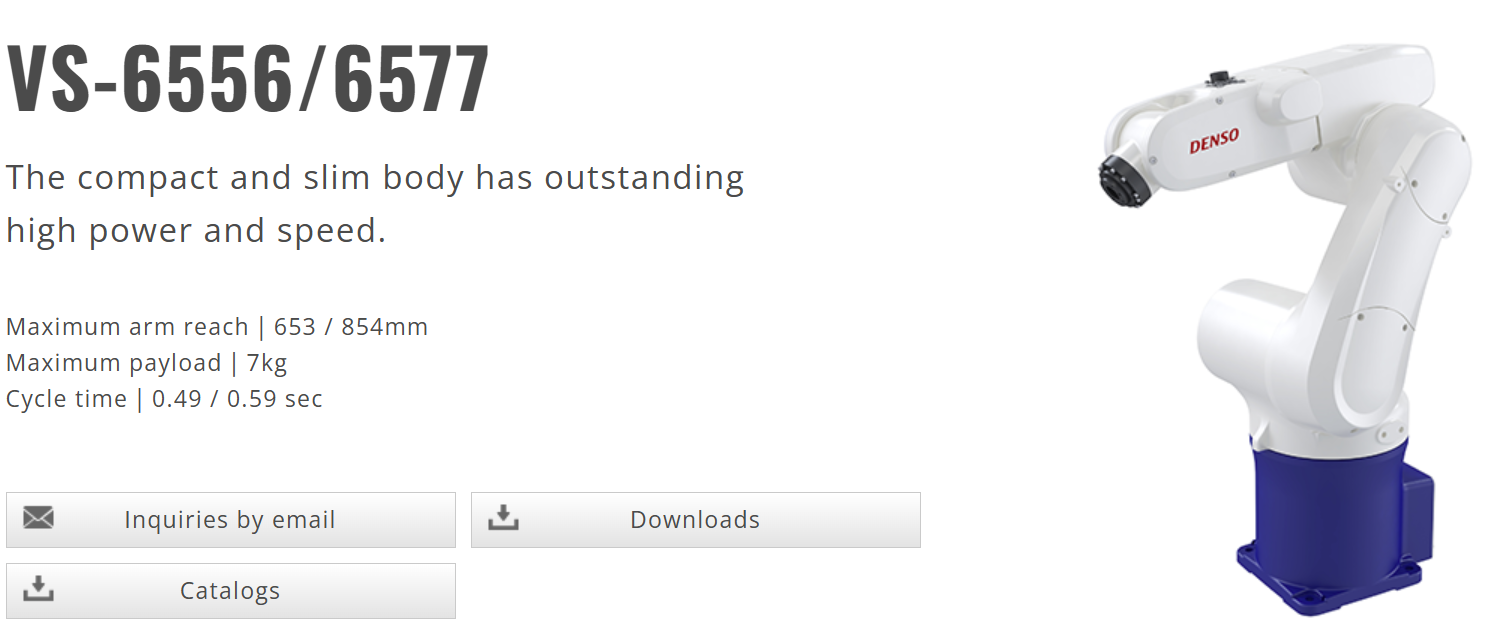
\includegraphics[width=1\linewidth]{Images/Methodologies/denso_arm_1.png}
    \caption{Cánh tay robot VS6577, hình ảnh lấy từ trang web nhà sản xuất}
    \label{fig:placeholder}
\end{figure}

Khi xem xét về đặc tả kĩ thuật của cánh tay, ta thấy thêm một số thông số ấn tượng về khả năng của cánh tay này:

\begin{longtblr}[
caption = {Thông số kĩ thuật của cánh tay Robot Denso VS-6577},
label = {tblr:my-table},
entry = {Thông số kĩ thuật của cánh tay Robot Denso VS-6577}
]{
hlines,vlines,
colspec = {X[1,c]X[3,l]},
columns = {valign = m},
}
Thông số kĩ thuật & Giá trị \\
Số trục & 6 \\
Độ dài cánh tay & 770mm \\
Độ lệch cánh tay & J1 (xoay): 75mm, J3 (cánh tay trước): 90mm \\
Vùng hoạt động tối đa & R = 934mm (tính phần mặt của end-effector), R=854mm (Tính phần trung tâm của J4, J5, J6) \\ 
Góc giới hạn & J1:±170°, \newline
                J2:+135°, -100°, \newline
                J3:+169°, -119°, \newline
                J4:±190°, \newline
                J5:±120°, \newline
                J6:±360° \\
Tải trọng tối đa & 7kg (với phần cổ cánh tay nghiêng xuống 1 góc khoảng 45°)\\
Nhận diện vị trí & Bộ Absolute Encoder\\
Động cơ xoay và phanh & AC motor cho toàn bộ các trục, phanh cho trục J2 tới J4\\
Khối lượng & ~ 36kg\\ 
Độ chính xác lặp lại & Với mỗi hướng X, Y và Z ±0.03mm\\
... & \\
\end{longtblr}

% 2 sub figure
\begin{figure}[H]
\centering
\begin{subfigure}{0.45\textwidth}
    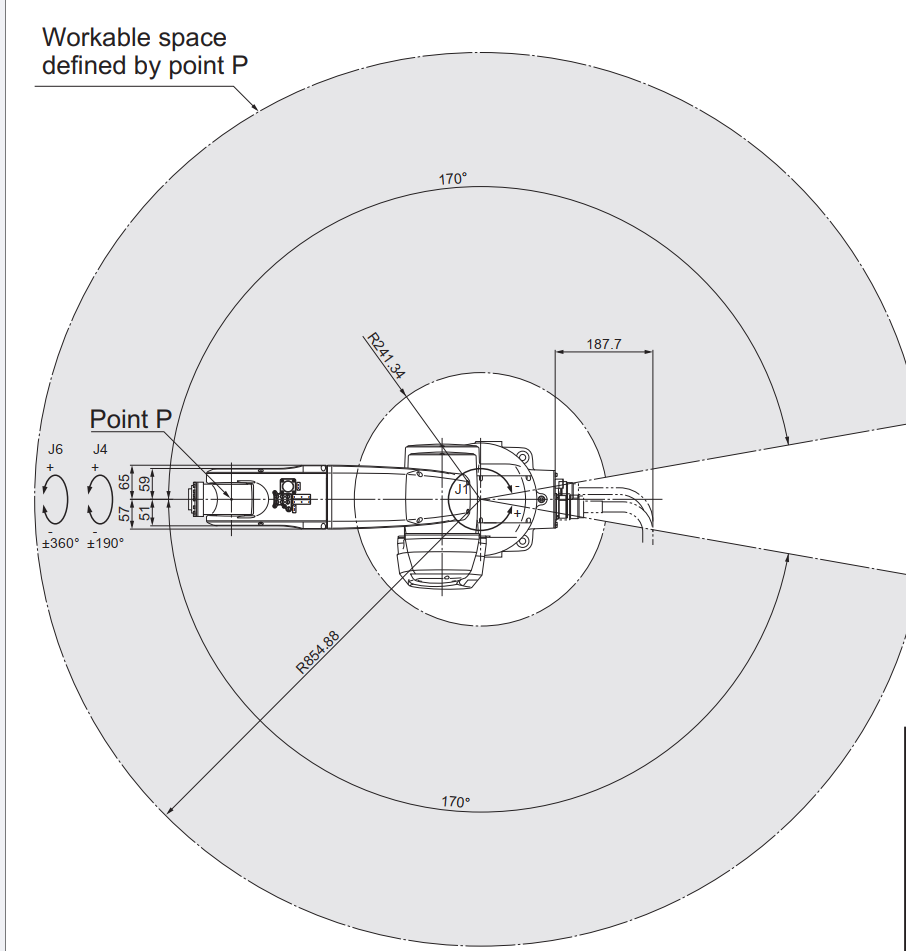
\includegraphics[width=\textwidth]{Images/Methodologies/denso_arm_2.png}
    %\caption{Train YOLO11-n}
\end{subfigure}
\hfill
\begin{subfigure}{0.45\textwidth}
    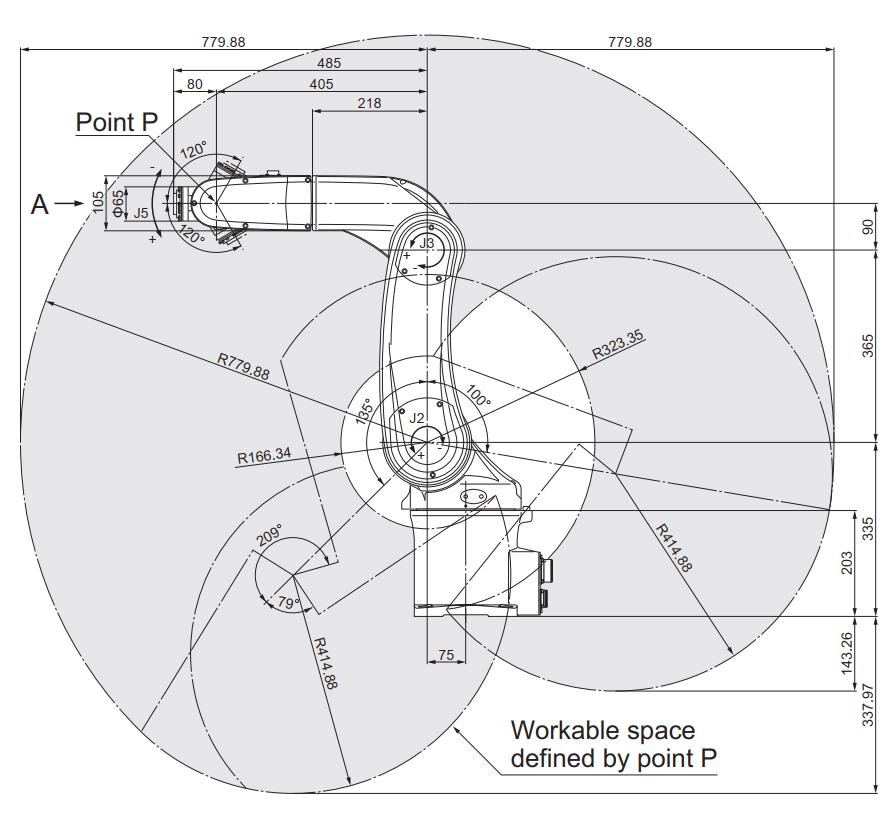
\includegraphics[width=\textwidth]{Images/Methodologies/denso_arm_3.png}
    %\caption{Train YOLO11-s}
\end{subfigure}
\hfill
\caption{Tầm hoạt động của cánh tay robot Denso từ nhà sản xuất}
\label{fig:denso_dimension}
\end{figure}

Với kích thước vừa phải và tương đối nhỏ gọn, cánh tay Denso VS6577 có sự linh hoạt tốt nhờ tầm hoạt động rộng ở từng trục, qua đó tạo nên vùng hoạt động lên tới 93.4cm tính cả phần mặt của end effector (phần đỉnh của cánh tay). Điều này giúp robot có thể dễ dàng tiếp cận và thao tác ở nhiều vị trí, góc độ khác nhau, đáp ứng tốt các yêu cầu ứng dụng đa dạng trong môi trường công nghiệp. Hơn nữa, độ chính xác lặp lại đạt ±0,03 mm (theo tài liệu kỹ thuật mới nhất), đảm bảo các thao tác lặp đi lặp lại đều đạt độ chính xác gần như tuyệt đối. Cánh tay Denso VS6577 là một lựa chọn tuyệt vời cho các ứng dụng trong môi trường nhà máy, công nghiệp, nơi sự chính xác và ổn định là yếu tố then chốt.

\section{Máy tính điều khiển RC5}

Bộ điều khiển RC5 của DENSO là một trong những giải pháp điều khiển robot công nghiệp nổi bật, được sử dụng rộng rãi trong các dây chuyền tự động hóa hiện đại trên toàn cầu. Được phát triển bởi DENSO – tập đoàn hàng đầu Nhật Bản về công nghệ tự động hóa và robot công nghiệp – RC5 không chỉ đáp ứng các tiêu chuẩn kỹ thuật khắt khe mà còn mang lại sự linh hoạt, độ tin cậy và khả năng tích hợp cao cho nhiều ứng dụng sản xuất khác nhau.

Hiện tại, bộ điều khiển Denso RC5 đang đóng vai trò điều khiển trực tiếp các trục xoay của cánh tay robot VS-6577. 

\begin{figure}[H]
    \centering
    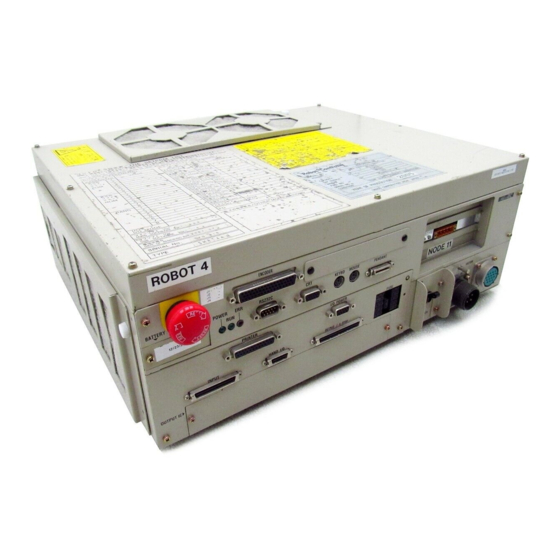
\includegraphics[width=0.7\linewidth]{Images/Methodologies/rc5_image.jpg}
    \caption{Máy tính điều khiển RC5}
    \label{fig:placeholder}
\end{figure}

Bộ điều khiển RC5 được thiết kế với nhiều phiên bản khác nhau, nhằm mục tiêu tối ưu cho từng loại robot khác nhau. Trong trường hợp hiện tại, bộ điều khiển RC5 có mã là RC5-VSE6B, trong đó "VSE" tức tương thích với dòng robot VS-E, "6" cho biết số trục điều khiển được là 6 trục, và "B" cho biết encoder được kết nối tới cổng CN12. Chi tiết vị trí của các cổng đầu vào sẽ được trình bày ở ảnh dưới:

\begin{figure}[H]
    \centering
    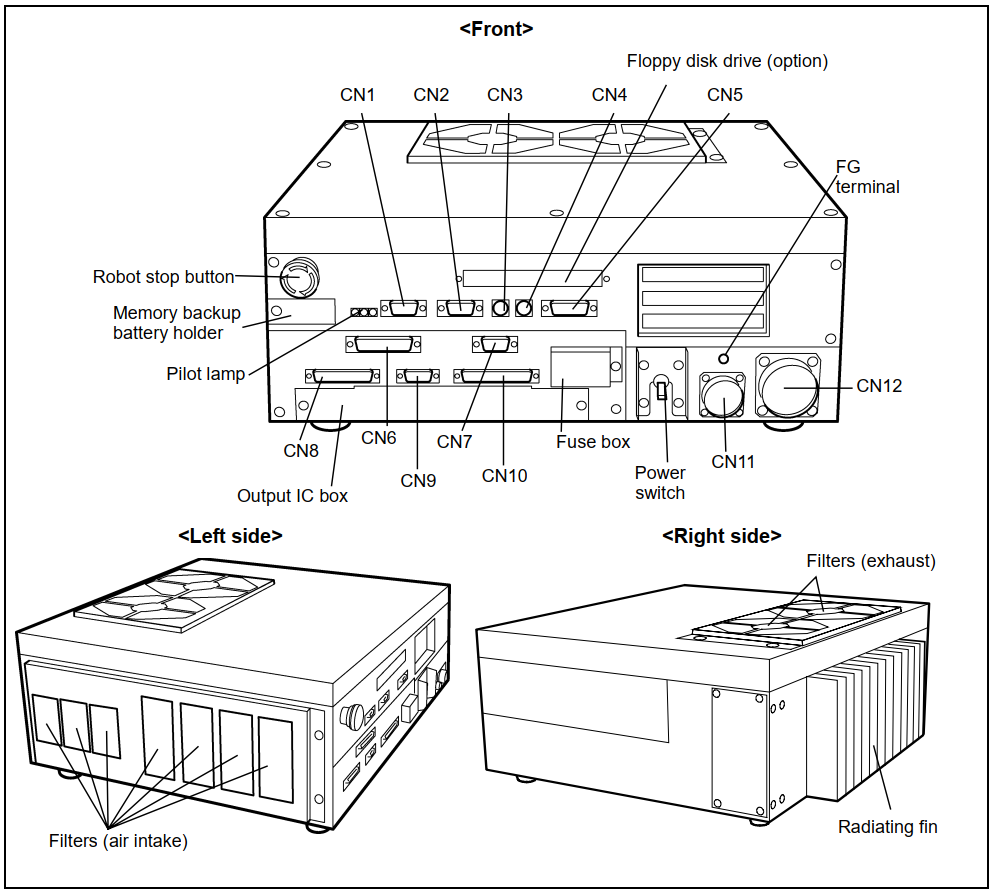
\includegraphics[width=1\linewidth]{Images/Methodologies/rc5_design.png}
    \caption{Vị trí các cổng nối của máy RC5}
    \label{fig:placeholder}
\end{figure}

\begin{longtblr}[
caption = {Ý nghĩa các cổng đầu vào trên máy điều khiển RC5},
label = {tblr:my-table},
entry = {Ý nghĩa các cổng đầu vào trên máy điều khiển RC5}
]{
hlines,vlines,
colspec = {X[1,c]X[1.5,c]X[2,l]X[1,c]X[1,c]X[2,l]},
columns = {valign = m},
}
\textbf{Số hiệu} & \textbf{Ký hiệu} & \textbf{Tên} & \textbf{Số hiệu} & \textbf{Ký hiệu} & \textbf{Tên} \\
CN1 & RS232C & Cổng giao tiếp nối tiếp & CN7 & I/O POWER & Cổng nguồn cho I/O \\
CN2 & CRT & Cổng màn hình CRT & CN8 & INPUT & Cổng đầu vào người dùng hoặc hệ thống (PLC) \\
CN3 & KEYBD & Cổng bàn phím & CN9 & HAND I/O & Cổng I/O cho End effector \\
CN4 & MOUSE & Cổng chuột PS/2 & CN10 & OUTPUT & Cổng đầu ra người dùng hoặc hệ thống (PLC) \\
CN5 & PENDANT & Cổng tay dạy (teach pendant) & CN11 & INPUT AC & Cổng nguồn xoay chiều \\
CN6 & PRINTER & Cổng máy in (không sử dụng) & CN12 & MOTOR & Cổng động cơ/bộ mã hóa \\
\end{longtblr}

Với việc có một lượng lớn các cổng kết nối, người dùng có sự linh hoạt trong việc tích hợp nó vào chu trình điều khiển hiện có. Không chỉ đơn thuần là điều khiển cánh tay robot, RC5 cũng có thể được sử dụng để điều khiển thêm các đầu gắp (end effector), kết nối với hệ thống PLC, kết nối với thiết bị "teach pendant", điều khiển I/O của nhiều thiết bị khác và hơn hết là cho phép kết nối với PC / thiết bị hỗ trợ quan sát (vision device) thông qua cổng giao tiếp RS232. 

\begin{longtblr}[
caption = {Bảng thông số kĩ thuật của máy điều khiển RC5 cho cánh tay robot VS-6577},
label = {tblr:my-table},
entry = {Bảng thông số kĩ thuật của máy điều khiển RC5 cho cánh tay robot VS-6577}
]{
hlines,vlines,
colspec = {X[1,c]X[3,l]},
columns = {valign = m},
}
\textbf{Mục} & \textbf{Thông số kỹ thuật} \\
Hệ thống điều khiển (GHI CHÚ 1) & PTP, CP tuyến tính 3 chiều, tròn 3 chiều \\
Số trục điều khiển (GHI CHÚ 1) & V*-D/E: Tối đa 6 trục đồng thời \\
Hệ thống truyền động & Tất cả các trục: Servo AC kỹ thuật số hoàn toàn \\
Dung lượng bộ nhớ & 1.25 MB (tương đương 5000 bước, 13.000 điểm) \\
Ngôn ngữ sử dụng & Ngôn ngữ robot DENSO (tuân theo SLIM) \\
Số chương trình dạy có thể tải vào bộ nhớ & 255 \\
Hệ thống dạy học & 1) Dạy từ xa 2) Nhập số liệu (MDI) \\
\SetCell[r=2]{c} Tín hiệu ngoài (I/O) & Tín hiệu vào: 20 điểm mở cho người dùng (PLC 12, tay vào 8) + 36 điểm hệ thống cố định\\ 
 & Tín hiệu ra: 32 điểm mở cho người dùng (PLC 24, tay ra 8) + 33 điểm hệ thống cố định \\
\SetCell[r=2]{c} Giao tiếp ngoài & RS-232C: 1 đường \\ 
& Ethernet: 1 đường (tùy chọn) \\
Chức năng hẹn giờ & 0.02 đến 10 giây (đơn vị 1/60 giây) \\
Chức năng tự chẩn đoán & Quá giới hạn, lỗi servo, lỗi bộ nhớ, lỗi đầu vào, v.v. \\
\SetCell[r=2]{c} Hiển thị lỗi & Mã lỗi hiển thị qua I/O ngoài hoặc bảng điều khiển (tùy chọn) \\
 & Thông báo lỗi hiển thị bằng tiếng Anh trên tay dạy (tùy chọn) \\
Nguồn điện & RC5 cho VS-D/E, H*-D/E, XYC-D: 1 pha, 230 VAC-10\% đến 230 VAC+10\%, 50/60 Hz\\
Công suất tiêu thụ (GHI CHÚ 1) & VS-E: 1.9 kVA\\ 
\SetCell[r=2]{c} Điều kiện môi trường (khi hoạt động) & Nhiệt độ: 0 đến 40°C\\ 
 & Độ ẩm: Dưới 90\% RH (không ngưng tụ) \\
Mức độ bảo vệ & IP20 \\
\SetCell[r=3]{c} Cáp (tùy chọn) & Cáp điều khiển robot: VS-D, H*-D, XYC-D: 3 m, 6 m (tùy chọn) \\ 
& Cáp I/O: 8 m, 15 m\\ 
& Cáp nguồn: 5 m \\
Khối lượng & VS-D/E, VC-E, HS-E: Khoảng 17 kg\\
\end{longtblr}

\begin{itemize}
    \item \textbf{Hệ thống điều khiển} của RC5 hỗ trợ các chế độ chuyển động PTP (Point-to-Point), CP (Continuous Path) với khả năng điều khiển tuyến tính và tròn trong không gian 3 chiều. Điều này cho phép RC5 đáp ứng tốt các yêu cầu chuyển động phức tạp trong các ứng dụng lắp ráp, hàn, sơn, hoặc xử lý vật liệu chính xác cao.
    \item \textbf{Dung lượng bộ nhớ} 1.25 MB cho phép lưu trữ tới 5000 bước chương trình và 13.000 điểm tọa độ, đáp ứng nhu cầu lập trình các chu trình phức tạp, đa nhiệm vụ. Số lượng chương trình dạy tối đa là 255, giúp người dùng dễ dàng quản lý và chuyển đổi giữa các tác vụ sản xuất khác nhau.
    \item \textbf{Khả năng tự chuẩn đoán lỗi} cũng là một tính năng quan trọng để đảm bảo việc vận hành robot được an toàn.
    \item Về \textbf{Ngôn ngữ sử dụng}, Ngôn ngữ robot DENSO, hay còn gọi là WINCAPS phiên bản 1 được sử dụng để có thể lập trình ngay trên máy RC5, tận dụng những hàm hỗ trợ về nhiều khía cạnh như input/ouput, ghi log, chuyển động cánh tay robot gồm thay đổi góc xoay, thay đổi tốc độ, thay đổi gia tốc, thay đổi vị trí.... Ngôn ngữ lập trình này cũng cung cấp đầy đủ các công cụ lập trình cần thiết như vòng lặp, điều kiện, khai báo và sử dụng biến, biến toàn cục và biến cục bộ. 
\end{itemize}
  
Tóm lại, máy tính điều khiển RC5 là một bộ điều khiển không thể thiếu để hoạt động cùng với cánh tay robot VS-6577, giúp giải quyết sự phức tạp trong điều khiển các bộ motor trong cánh tay robot sao cho mượt mà, hiệu quả và chính xác, đáp ứng những yêu cầu khắc khe về thời gian cũng như độ tin cậy trong phần lớn những ứng dụng trong môi trường công nghiệp.

\section{Gripper-A và Driver-Hat-A}

\subsection{Tay gắp Gripper-A}

Tay gắp (gripper) là một loại thiết bị cuối (end-effector) phổ biến được lắp vào đầu cánh tay robot, có vai trò trực tiếp tương tác với đối tượng trong môi trường làm việc. Tùy theo ứng dụng, gripper có thể có nhiều dạng khác nhau: kiểu ngón tay song song (parallel jaw gripper), kiểu hút chân không, kiểu nam châm điện, hay thiết kế lấy cảm hứng từ bàn tay người. Trong đề tài này, tay gắp được chọn là loại \textbf{parallel jaw gripper} (hai hàm song song) với cơ cấu điều khiển bằng servo motor.

\begin{figure}[H]
    \centering
    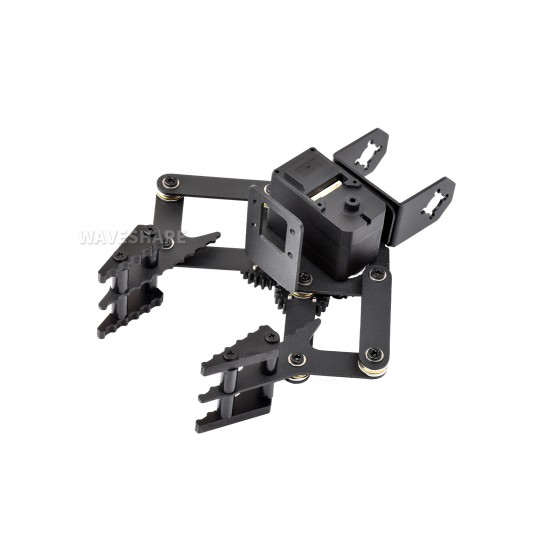
\includegraphics[width=0.6\linewidth]{Images/Methodologies/gripper_a.jpg}
    \caption{Tay gắp Gripper-A}
    \label{fig:gripper_a}
\end{figure}

Tay gắp được điều khiển thông qua một servo motor duy nhất, có tên khớp (joint) là \lstinline[style=inlinecode]{gripper_gear_right_joint}. Phạm vi chuyển động của servo nằm trong khoảng từ \textbf{5°} (vị trí đóng hoàn toàn, tương đương 0.087266 rad) đến \textbf{85°} (vị trí mở hoàn toàn, tương đương 1.48353 rad). Cơ cấu bánh răng bên trong tay gắp chuyển đổi góc xoay của servo thành chuyển động tịnh tiến của hai hàm gắp theo hướng đối xứng nhau, đảm bảo vật thể được kẹp giữ ở chính giữa.

\subsection{Driver-Hat-A}

Driver-Hat-A là một bo mạch điều khiển servo được thiết kế dưới dạng \textit{hat} (mũ gắn lên), tương thích với các máy tính nhúng như Raspberry Pi hoặc Jetson. Bo mạch này đóng vai trò cầu nối trung gian giữa PC Controller và servo motor bên trong tay gắp, nhận lệnh điều khiển qua giao tiếp \textbf{UART} (cổng \lstinline[style=inlinecode]{/dev/ttyACM0}, tốc độ 115200 bps) và xuất tín hiệu điều khiển servo tương ứng.

\begin{figure}[H]
    \centering
    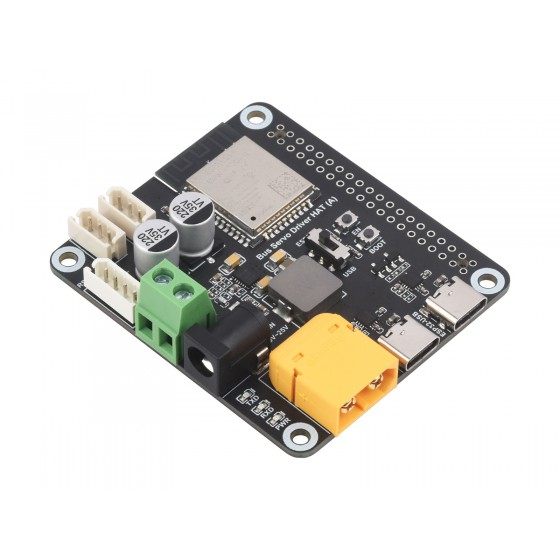
\includegraphics[width=0.5\linewidth]{Images/Methodologies/driver_hat_a.jpg}
    \caption{Bo mạch Driver-Hat-A}
    \label{fig:driver_hat_a}
\end{figure}

\textbf{Giao thức truyền thông JSON}

Driver-Hat-A sử dụng giao thức lệnh dạng chuỗi \textbf{JSON} (JavaScript Object Notation), giúp lệnh truyền đi dễ đọc, dễ kiểm tra và mở rộng. Lệnh điều khiển vị trí servo có định dạng:

\begin{lstlisting}[language=json]
{"T":121,"angle":0.67,"spd":100,"acc":10}
\end{lstlisting}

Trong đó:
\begin{itemize}
    \item \lstinline[style=inlinecode]{"T":121}: Mã lệnh điều khiển vị trí servo.
    \item \lstinline[style=inlinecode]{"angle"}: Góc xoay mục tiêu của servo tính bằng \textbf{radian}.
    \item \lstinline[style=inlinecode]{"spd"}: Tốc độ xoay, trong khoảng từ 0 đến 4096 (0 = tốc độ tối đa).
    \item \lstinline[style=inlinecode]{"acc"}: Gia tốc, trong khoảng từ 0 đến 254 (0 = gia tốc tối đa).
\end{itemize}

Để truy vấn trạng thái hiện tại của servo, PC Controller gửi lệnh:
\begin{lstlisting}[language=json]
{"T":105}
\end{lstlisting}

Driver-Hat-A sẽ phản hồi với gói tin chứa đầy đủ thông tin:
\begin{lstlisting}[language=json]
{"T":1051,"pos":3138,"speed":0,"load":-104,"voltage":124,
 "current":4,"temper":45,"mode":0}
\end{lstlisting}

Trường \lstinline[style=inlinecode]{"pos"} chứa vị trí hiện tại của servo dưới dạng \textbf{giá trị encoder step} (không phải góc độ trực tiếp). Để chuyển đổi sang góc độ (đơn vị độ), ta áp dụng công thức:

\begin{align*}
angle\_deg = (pos - 1024) \times \frac{360}{4096}
\end{align*}

Ngoài vị trí, các thông số phụ như \lstinline[style=inlinecode]{speed} (vận tốc), \lstinline[style=inlinecode]{load} (tải trọng), \lstinline[style=inlinecode]{voltage} (điện áp), \lstinline[style=inlinecode]{current} (dòng điện) và \lstinline[style=inlinecode]{temper} (nhiệt độ) cũng được trả về, giúp hệ thống có thể phát hiện sự cố trong quá trình hoạt động. Đặc biệt, giá trị \lstinline[style=inlinecode]{load} rất hữu ích để phát hiện khi tay gắp đang kẹp vật thể (tải trọng tăng đột biến), hỗ trợ cơ chế dừng tự động tránh làm hỏng vật gắp.


\section{Khái niệm về động học robot}

Động học (kinematics) là một nhánh của cơ học nghiên cứu về chuyển động của vật thể mà không xét đến nguyên nhân gây ra chuyển động đó (tức là không xét đến lực). Trong robot học, động học tập trung vào việc mô tả vị trí, hướng, vận tốc và gia tốc của các bộ phận robot dựa trên các biến khớp (joint variables) và cấu trúc hình học của hệ thống.

Đối với cánh tay robot sáu trục như Denso VS-6577, toàn bộ cấu trúc cơ khí có thể được mô hình hóa như một chuỗi các khâu cứng nối tiếp nhau qua các khớp xoay (revolute joints). Trạng thái của robot tại mọi thời điểm được đặc trưng bởi vector các giá trị khớp $\mathbf{q} = [q_1, q_2, q_3, q_4, q_5, q_6]^T$, trong đó $q_i$ là góc xoay của khớp thứ $i$. Có hai bài toán cơ bản trong động học robot: \textbf{động học thuận} và \textbf{động học nghịch}.

\subsection{Động học thuận}

Động học thuận (Forward Kinematics - FK) là quá trình xác định vị trí và hướng của end-effector trong không gian Cartesian dựa trên tập giá trị khớp đã biết và các tham số hình học của robot. Đây là bài toán có \textbf{nghiệm duy nhất}: với một cấu hình khớp xác định, chỉ tồn tại đúng một tư thế tương ứng của end-effector.

Phương pháp phổ biến nhất để giải bài toán động học thuận là sử dụng \textbf{quy ước Denavit–Hartenberg (DH)}. Theo quy ước này, mỗi khớp $i$ được gán một hệ tọa độ cục bộ, và mối quan hệ giữa hai hệ tọa độ liền kề được mô tả bởi bốn tham số DH: $a_i$, $\alpha_i$, $d_i$, $\theta_i$. Ma trận biến đổi đồng nhất giữa hai khâu liền kề được xác định bởi:

\begin{equation}
^{i-1}T_i = 
\begin{bmatrix}
\cos\theta_i & -\sin\theta_i\cos\alpha_i &  \sin\theta_i\sin\alpha_i & a_i\cos\theta_i \\
\sin\theta_i &  \cos\theta_i\cos\alpha_i & -\cos\theta_i\sin\alpha_i & a_i\sin\theta_i \\
0            &  \sin\alpha_i             &  \cos\alpha_i             & d_i             \\
0            &  0                        &  0                        & 1
\end{bmatrix}
\end{equation}

Tư thế của end-effector so với hệ tọa độ gốc được tính bằng tích liên tiếp của các ma trận biến đổi:

\begin{equation}
^0T_6 = {^0T_1} \cdot {^1T_2} \cdot {^2T_3} \cdot {^3T_4} \cdot {^4T_5} \cdot {^5T_6}
\end{equation}

Ma trận $^0T_6 \in \mathbb{R}^{4 \times 4}$ là \textbf{ma trận biến đổi đồng nhất} chứa đầy đủ thông tin về vị trí (cột cuối, 3 hàng đầu) và hướng (ma trận con $3\times3$ góc trên trái) của end-effector. Động học thuận là nền tảng cho việc hiển thị, mô phỏng robot và cũng là cơ sở để kiểm tra kết quả của bài toán động học nghịch.

\subsection{Động học nghịch}

Động học nghịch (Inverse Kinematics - IK) là quá trình xác định tập giá trị khớp $\mathbf{q}$ cần thiết để đưa end-effector đến một tư thế mong muốn $\mathbf{x} = [x, y, z, \phi, \psi, \theta]^T$ cho trước trong không gian Cartesian. Đây là bài toán \textbf{ngược với} động học thuận, thường phức tạp hơn nhiều vì:

\begin{itemize}
    \item Bài toán có thể có \textbf{nhiều nghiệm} (nhiều cấu hình khớp khác nhau đều đưa end-effector đến cùng một tư thế), \textbf{một nghiệm duy nhất}, hoặc \textbf{không có nghiệm} (tư thế mục tiêu nằm ngoài vùng làm việc).
    \item Đối với robot 6 bậc tự do thông thường, có thể tồn tại đến 16 nghiệm IK khác nhau tùy theo cấu hình cơ học.
    \item Hệ phương trình phi tuyến không phải lúc nào cũng có nghiệm giải tích (closed-form) và thường phải dùng phương pháp số (iterative).
\end{itemize}

Có hai nhóm phương pháp chính để giải bài toán IK:

\begin{enumerate}
    \item \textbf{Phương pháp giải tích (Closed-form / Analytical IK)}: Khai thác cấu trúc hình học đặc thù của robot (ví dụ: ba trục cuối giao nhau tại một điểm – cấu hình cổ tay cầu - spherical wrist) để tìm nghiệm dạng công thức toán học. Phương pháp này cho kết quả nhanh và chính xác nhưng chỉ áp dụng được cho một số kiểu robot nhất định.
    
    \item \textbf{Phương pháp số (Numerical IK)}: Sử dụng các thuật toán lặp như phương pháp Jacobian pseudo-inverse, thuật toán gradient descent hoặc các phương pháp tối ưu hóa để hội tụ đến nghiệm. Phương pháp này tổng quát hơn nhưng có thể chậm hơn, phụ thuộc vào điểm khởi tạo và có thể không hội tụ gần các điểm kỳ dị (singularity).
\end{enumerate}

Trong đề tài, bài toán IK được giải quyết thông qua thư viện plugin của MoveIt2, cụ thể là \textbf{KDL Kinematics Plugin} (\lstinline[style=inlinecode]{kdl_kinematics_plugin/KDLKinematicsPlugin}) – một solver IK số dựa trên thư viện Kinematics and Dynamics Library của Orocos, với thời gian tìm kiếm và timeout được cấu hình trong file \lstinline[style=inlinecode]{kinematics.yaml}:

\begin{lstlisting}
denso_arm:
  kinematics_solver: kdl_kinematics_plugin/KDLKinematicsPlugin
  kinematics_solver_search_resolution: 0.005
  kinematics_solver_timeout: 0.005
\end{lstlisting}

Khi ứng dụng VR hoặc module Remote Control yêu cầu cánh tay di chuyển đến một tư thế Cartesian xác định, MoveIt2 sẽ tự động gọi plugin IK này để tính toán cấu hình khớp tương ứng, sau đó lập kế hoạch quỹ đạo an toàn và thực thi.


\section{Giao thức UART}

UART (Universal Asynchronous Receiver/Transmitter – Bộ truyền nhận dữ liệu nối tiếp bất đồng bộ) là một trong những giao thức truyền thông nối tiếp cơ bản và lâu đời nhất, được sử dụng rộng rãi trong lĩnh vực điện tử, hệ thống nhúng, máy tính và các thiết bị ngoại vi. Ra đời từ những năm 1970 với sự xuất hiện của chip WD1402A của Western Digital, UART đã trở thành nền tảng cho việc truyền dữ liệu giữa các thiết bị số mà không cần đến tín hiệu đồng hồ chung.

Về bản chất, UART là một phần cứng hoặc module tích hợp trong vi điều khiển, máy tính, hoặc có thể là một IC độc lập, đảm nhiệm việc chuyển đổi dữ liệu song song từ CPU hoặc bus dữ liệu thành dữ liệu nối tiếp để truyền đi, và ngược lại, chuyển đổi dữ liệu nối tiếp nhận được thành song song để xử lý tiếp theo. Giao tiếp UART sử dụng hai dây chính: TX (Transmit – truyền) và RX (Receive – nhận), cùng với dây nối đất chung, giúp đơn giản hóa kết nối vật lý giữa các thiết bị.

\begin{figure}[H]
    \centering
    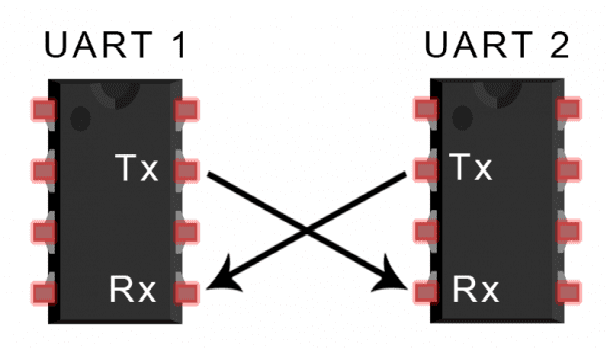
\includegraphics[width=0.8\linewidth]{Images/Methodologies/uart_2.png}
    \caption{Kết nối UART}
    \label{fig:placeholder}
\end{figure}

Điểm nổi bật của UART là khả năng truyền dữ liệu không đồng bộ, tức là không cần tín hiệu clock chung giữa hai thiết bị truyền và nhận. Thay vào đó, các thiết bị phải được cấu hình cùng tốc độ truyền (baud rate) và cùng định dạng khung dữ liệu để đảm bảo việc truyền nhận chính xác. Để nhận biết việc nhận dữ liệu, UART sử dụng các start bit và stop bit vào gói dữ liệu, giúp xác định điểm bắt đầu và điểm kết thúc của một dữ liệu được truyền trên dường dây.

Định dạng của một gói tin UART thường sẽ gồm 4 phần: Start bit, data frame, parity và stop bit:

\begin{figure}[H]
    \centering
    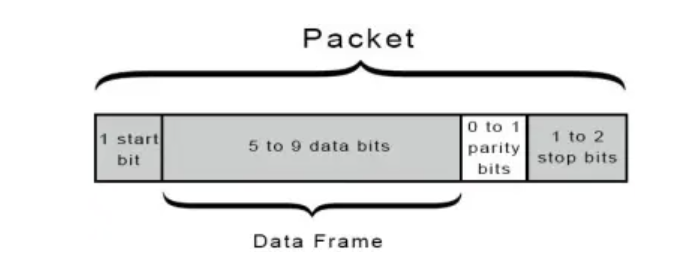
\includegraphics[width=0.8\linewidth]{Images/Methodologies/uart_1.png}
    \caption{Định dạng một gói tin (package) của UART}
    \label{fig:placeholder}
\end{figure}

\begin{enumerate}
    \item \textbf{Start bit}: Thông thường, đường truyền dữ liệu UART sẽ ở mức điện áp cao khi không có dữ liệu. Lúc bắt đầu truyền dữ liệu, UART sẽ kéo đường truyền xuống mức thấp trong một chu kì xung nhịp. Đây chính là Start bit của quá trình truyền nhận. Thiết bị UART ở phía nhận khi nhận thấy tín hiệu xuống thấp lần đầu tiên sẽ bắt đầu đọc các dữ liệu được truyền sau đó
    \item \textbf{Data Frame}: Đây là khu vực chứa dữ liệu cần truyền. Độ dài của dữ liệu có thể từ 5 tới 9 bit, với 9 bit trong trường hợp không sử dụng Parity bit. 
    \item \textbf{Parity Bit}: Parity bit chỉ có một bit, cho biết số lượng bit 1 trong khung dữ liệu là số chẵn hay số lẻ. Mục tiêu của Parity bit là bảo đảm sự toàn vẹn dữ liệu ở mức tương đối, như một cách để thiết bị nhận biết rằng có bất kì dữ liệu nào đã bị thay đổi trong quá trình truyền hay không. 
    \item \textbf{Stop bits}: Stop bits có độ dài từ 1 tới 2 bit, khi đó UART sẽ gửi tín hiệu điện áp từ thấp lên cao trong ít nhất hai bit, đánh dấu sự kết thúc của gói tin truyền nhận.
\end{enumerate}

\textbf{Ưu điểm của giao thức UART}

Khi nhắc tới UART, ta có thể nhận thấy ngay nhiều ưu điểm của giao thức này như:

\begin{itemize}
    \item Kết nối đơn giản, chỉ sử dụng hai dây truyền dữ liệu cho giao tiếp điểm - điểm (Point to Point)
    \item Không cần đồng bộ với xung clock để hoạt động
    \item Có cơ chế kiểm tra lỗi thông qua bit chẵn lẻ
    \item Tốc độ truyền đa dạng, với baud rate từ 110 bps lên tới 921600 bps
    \item Phương pháp truyền đơn giản và giá thành thấp
\end{itemize}

\textbf{Nhược điểm của giao thức UART}

Tuy vậy, sự đơn giản của UART cũng mang cho nó một số nhược điểm so với các giao thức khác:

\begin{itemize}
    \item Kích thước dữ liệu trong mỗi gói tin nhỏ, chỉ tối đa 9 bit
    \item Chỉ phù hợp cho kết nối Point to Point. Không phù hợp trong kết nối dạng Master-Slave cần điều khiển nhiều thiết bị cùng lúc
    \item Tốc độ tối đa sẽ thấp hơn SPI, I2C, bị ảnh hưởng bởi chiều dài dây và khả năng bị nhiễu
    \item Yêu cầu hai thiết bị phải có cùng baud rate, hoặc ít nhất sự chênh lệnh không vượt quá 10\%
\end{itemize}

\section{ROS2 - Robot Operating System}

ROS2 (Robot Operating System) là một hệ thống phần mềm mã nguồn mở dành cho robot, được phát triển bởi Willow Garage và hiện đang được duy trì bởi Open Robotics. Dù gọi mình là một hệ điều hành (Operating System), ROS 2 không thực sự là một hệ điều hành, mà cung cấp một khung làm việc (framework) gồm vô số các công cụ mạnh mẽ để phát triển các ứng dụng robot, cung cấp các công cụ và thư viện để giúp lập trình viên tạo ra các ứng dụng điều khiển robot, phân tích dữ liệu, xử lý hình ảnh và video, và tương tác với các thiết bị ngoại vi.

ROS 2 được thiết kế để hoạt động trên nhiều hệ điều hành khác nhau, bao gồm Linux, macOS và Windows. Nó cũng được tích hợp sẵn với các thư viện và công cụ phổ biến như OpenCV, PCL (Point Cloud Library) và TensorFlow.

ROS 2 có nhiều ưu điểm, bao gồm:
\begin{itemize}
    \item Tích hợp dễ dàng: ROS 2 có thể kết nối với các thiết bị phần cứng và phần mềm khác một cách dễ dàng, giúp người dùng tập trung vào phát triển ứng dụng chính thay vì việc tích hợp phần cứng.
    \item Hỗ trợ tương tác: ROS 2 cung cấp các công cụ để tương tác với robot, cho phép người dùng điều khiển robot trực tiếp và thu thập dữ liệu từ các cảm biến.
    \item Khả năng mở rộng: ROS 2 cho phép người dùng thêm các chức năng mới vào hệ thống một cách dễ dàng, bằng cách tạo các gói phần mềm mới hoặc sử dụng các gói phần mềm có sẵn.
\end{itemize}
ROS 2 là một công cụ quan trọng trong phát triển robot và trí tuệ nhân tạo. Nó được sử dụng rộng rãi trong nhiều lĩnh vực, bao gồm robot tự hành, robot y tế và robot công nghiệp. Trong đồ án này, máy tính nhúng Jetson Nano đã tích hợp sẵn những chương trình ROS cho phép ta phát triển ứng dụng trên đó dễ dàng hơn.
\begin{figure}[H]
    \centering
    
\includegraphics[width=0.6\textwidth]{Images/Methodologies/ros2_logo.png}
    \caption{Robot Operating System 2}
\end{figure}

ROS 2 là một trong những hệ thống hỗ trợ điều khiển robot không thể thiếu trong mọi ứng dụng thiết kế, phát triển và lập trình robot. Việc xây dựng ứng dụng điều khiển cánh tay sử dụng ROS là mục tiêu mà đề tài hướng tới trong giai đoạn tiếp theo. Ở giai đoạn hiện tại, do giới hạn về thời gian dùng để lắp ráp robot, chương trình điều khiển được xây dựng bằng Python ở mức cơ bản để chứng minh khả năng điều khiển và quan sát cách hoạt động thực tế của robot.

\subsection{Ros2-Control}

Ros2-Control là một framework cho việc điều khiển robot thời gian thực (real-time) trên nền tảng ROS2. Mục tiêu chính của Ros2-Control đó là thực hiện việc quản lý và điều khiển phần cứng của robot theo cách thức chuẩn hóa và mô dun hóa, qua đó giúp dễ dàng tích hợp phần cứng vào ứng dụng ROS2. Để làm được điều này, Ros2-Control định nghĩa một kiến trúc bao gồm bốn lớp: Controller, Controller Manager, Resource Manager và Hardware component. Sơ đồ kiến trúc theo Ros2-Control được thể hiện bên dưới:

\begin{figure}[H]
    \centering
    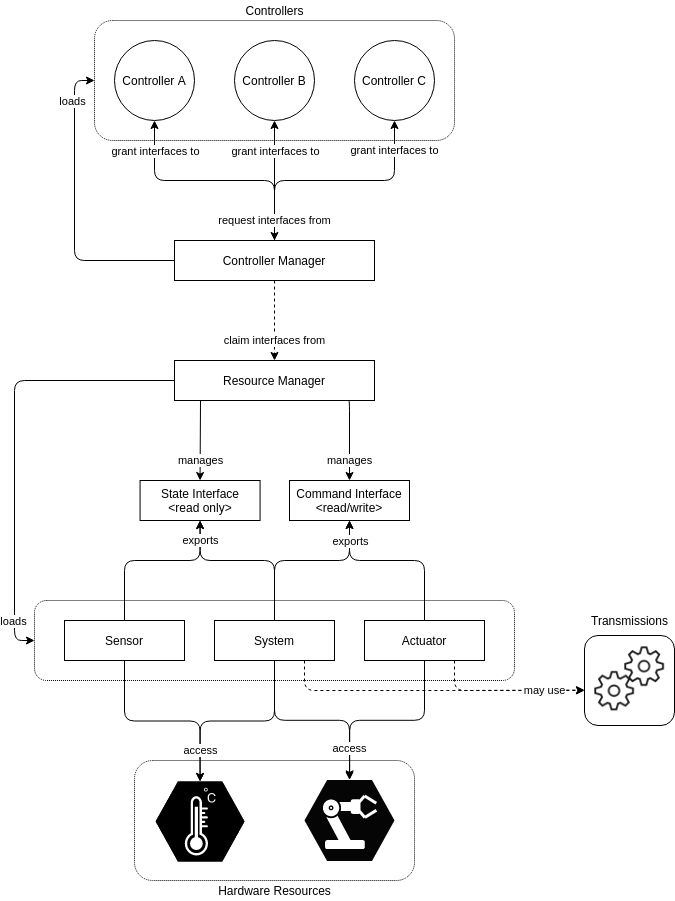
\includegraphics[width=0.9\textwidth]{Images/Methodologies/ros2_control_architect.png}
    \caption{Sơ đồ kiến trúc của Ros2-Control}
\end{figure}

\subsubsection{Controller Manager}
Controller Manager là thành phần kết nối các bộ điều khiển với lớp trừu tượng phần cứng trong framework \texttt{ros2\_control}, đồng thời đóng vai trò là điểm truy cập cho người dùng thông qua các dịch vụ ROS. Controller Manager được triển khai dưới dạng một node không có executor để có thể tích hợp vào thiết lập tùy chỉnh, nhưng thường khuyến nghị sử dụng node mặc định trong file \texttt{ros2\_control\_node} thuộc gói \texttt{controller\_manager}. Trong quá trình hoạt động, Controller Manager quản lý việc nạp, kích hoạt, hủy kích hoạt và gỡ bỏ các bộ điều khiển cùng với các \textbf{interface} mà chúng yêu cầu, đồng thời truy cập vào các thành phần phần cứng thông qua Resource Manager. Controller Manager đối chiếu giữa \textbf{interface} yêu cầu và \textbf{interface} cung cấp, cho phép bộ điều khiển truy cập phần cứng khi được bật hoặc báo lỗi nếu có xung đột. Vòng lặp điều khiển được thực thi bởi phương thức \texttt{update()}, nơi Controller Manager đọc dữ liệu từ phần cứng, cập nhật đầu ra của các bộ điều khiển đang hoạt động và ghi kết quả trở lại phần cứng.

\subsubsection{Resource Manager}
Resource Manager đảm nhận việc trừu tượng hóa phần cứng vật lý và driver của nó, gọi là \textit{hardware components}, cho framework \texttt{ros2\_control}. Resource Manager nạp các thành phần bằng thư viện \texttt{pluginlib}, quản lý vòng đời, trạng thái và \textbf{interface} lệnh của chúng. Nhờ lớp trừu tượng này, các thành phần phần cứng đã triển khai có thể được tái sử dụng mà không cần viết lại, đồng thời cho phép ứng dụng phần cứng linh hoạt cho \textbf{interface} trạng thái và lệnh. Trong vòng lặp điều khiển, Resource Manager giao tiếp với phần cứng thông qua các phương thức \texttt{read()} và \texttt{write()}.

\subsubsection{Controllers}
Các bộ điều khiển trong \texttt{ros2\_control} dựa trên lý thuyết điều khiển, so sánh giá trị tham chiếu với đầu ra đo được và tính toán đầu vào hệ thống dựa trên sai số. Chúng là các đối tượng kế thừa từ \texttt{ControllerInterface} trong gói \texttt{controller\_interface} và được xuất dưới dạng plugin bằng \texttt{pluginlib}. Ví dụ điển hình là \texttt{ForwardCommandController} trong repository \texttt{ros2\_controllers}. Vòng đời của bộ điều khiển dựa trên lớp \texttt{LifecycleNode}, vốn triển khai máy trạng thái được mô tả trong tài liệu \textit{Node Lifecycle Design}. Khi vòng lặp điều khiển chạy, phương thức \texttt{update()} được gọi để truy cập trạng thái phần cứng mới nhất và cho phép bộ điều khiển ghi dữ liệu vào \textbf{interface} lệnh phần cứng.

\subsubsection{Hardware Components}
Các thành phần phần cứng thực hiện giao tiếp với phần cứng vật lý và đại diện cho lớp trừu tượng của nó trong framework \texttt{ros2\_control}. 
Các thành phần này phải được xuất dưới dạng plugin bằng \texttt{pluginlib}. 
Resource Manager sẽ nạp động các plugin này và quản lý vòng đời của chúng.

Có ba loại thành phần cơ bản cho Hardware component:

\begin{itemize}
\item \textbf{{Hệ thống - System}}

Dùng cho phần cứng robot phức tạp (multi-DOF) như robot công nghiệp. Khác với Actuator, System có thể sử dụng truyền động phức tạp như là cánh tay robot hay bàn tay robot (humanoid robot's hand). Hardware component dạng System có khả năng đọc và ghi xuống thiết bị thực tế, và thường dùng khi chỉ có một kênh giao tiếp logic với phần cứng.

\item \textbf{{Cảm biến - Sensor}}
Dành cho phần cứng robot dùng để cảm nhận môi trường xung quanh như camera, cảm biến nhiệt độ, cảm biến màu sắc, không gian.... Các cảm biến thường chỉ Liên kết với một khớp. Đối với hardware dạng cảm biến, ta chỉ có thể đọc dữ liệu được truyền lên từ phần cứng

\item \textbf{{Bộ truyền động - Actuator}}
Bộ truyền động thường nói đến phần cứng robot đơn giản (1 trục tự do) như động cơ, van, v.v.  và chỉ liên kết với một khớp duy nhất. 
tương tự như System, Actuator cũng có khả năng đọc và ghi, tuy nhiên thao tác(\textit{đọc} không bắt buộc nếu không khả thi, ví dụ: điều khiển động cơ DC hay servo 
\end{itemize}

\subsection{MoveIt 2}

MoveIt 2 là một nền tảng phát triển tích hợp trong ROS 2, bao gồm nhiều gói chức năng phục vụ cho việc điều khiển cánh tay robot. Các chức năng này trải rộng từ lập kế hoạch chuyển động, thao tác, điều khiển, động học ngược, nhận thức 3D cho đến phát hiện va chạm, là một nền tảng trợ giúp đắc lực cho việc nhanh chóng xây dựng ứng dụng điều khiển cánh tay robot.

\begin{figure}[H]
    \centering
    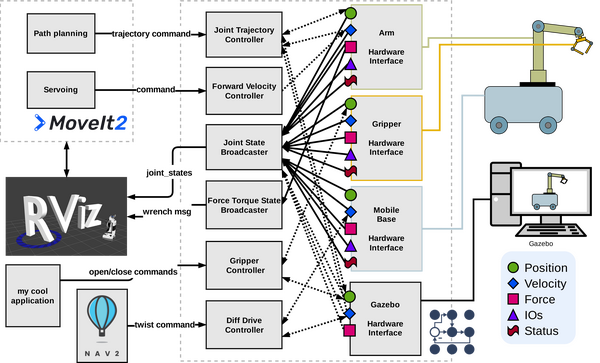
\includegraphics[width=1\textwidth]{Images/Methodologies/moveit_integration.png}
    \caption{MoveIt 2 được tích hợp cùng với Ros2-Control trong ứng dụng robotic}
\end{figure}

MoveIt 2 cung cấp khả năng lập kế hoạch chuyển động dựa trên OMPL (Open Motion Planning Library) cùng nhiều thư viện bên thứ ba, hỗ trợ đa dạng thuật toán và ràng buộc.  
Hệ thống động học ngược (IK) được triển khai thông qua cơ chế plug-in, cho phép sử dụng nhiều bộ giải IK khác nhau để nhanh chóng tính toán tư thế mục tiêu của cánh tay robot.  
Khả năng phát hiện và tránh va chạm được tích hợp sẵn, đảm bảo robot không va chạm với môi trường xung quanh trong quá trình lập kế hoạch và thực thi chuyển động.  
MoveIt 2 còn hỗ trợ cập nhật mô hình môi trường một cách linh hoạt, có thể nhận biết sự thay đổi của chướng ngại vật theo thời gian thực.  
Giao diện điều khiển chuyển động được kết nối chặt chẽ với phần cứng robot, giúp đảm bảo đường đi đã được lập kế hoạch có thể thực hiện chính xác.  
Ngoài ra, MoveIt 2 tích hợp với RViz 2, mang lại công cụ trực quan để tương tác, gỡ lỗi và hiển thị quá trình lập kế hoạch cũng như thực thi chuyển động ngay lập tức.

MoveIt 2 mang lại nhiều ưu điểm trong ứng dụng điều khiển robot với ROS2 như:
\begin{itemize}
    \item Nhờ kiến trúc truyền thông DDS của ROS 2, MoveIt 2 đạt được hiệu năng thời gian thực và độ tin cậy cao hơn đáng kể. 
    \item Thiết kế theo mô-đun giúp người dùng dễ dàng tải hoặc thay thế các thành phần khi cần, mang lại sự linh hoạt lớn.  
    \item MoveIt 2 có khả năng chạy trên nhiều hệ điều hành khác nhau như Ubuntu, Windows, cũng như nhiều nền tảng phần cứng.
    \item Cộng đồng phát triển toàn cầu của MoveIt 2 luôn tích cực đóng góp, liên tục cập nhật, mở rộng tính năng và cung cấp hỗ trợ kỹ thuật.
\end{itemize}

\section{Kính thực tế ảo Meta Quest 3}

\begin{figure}[H]
    \centering
    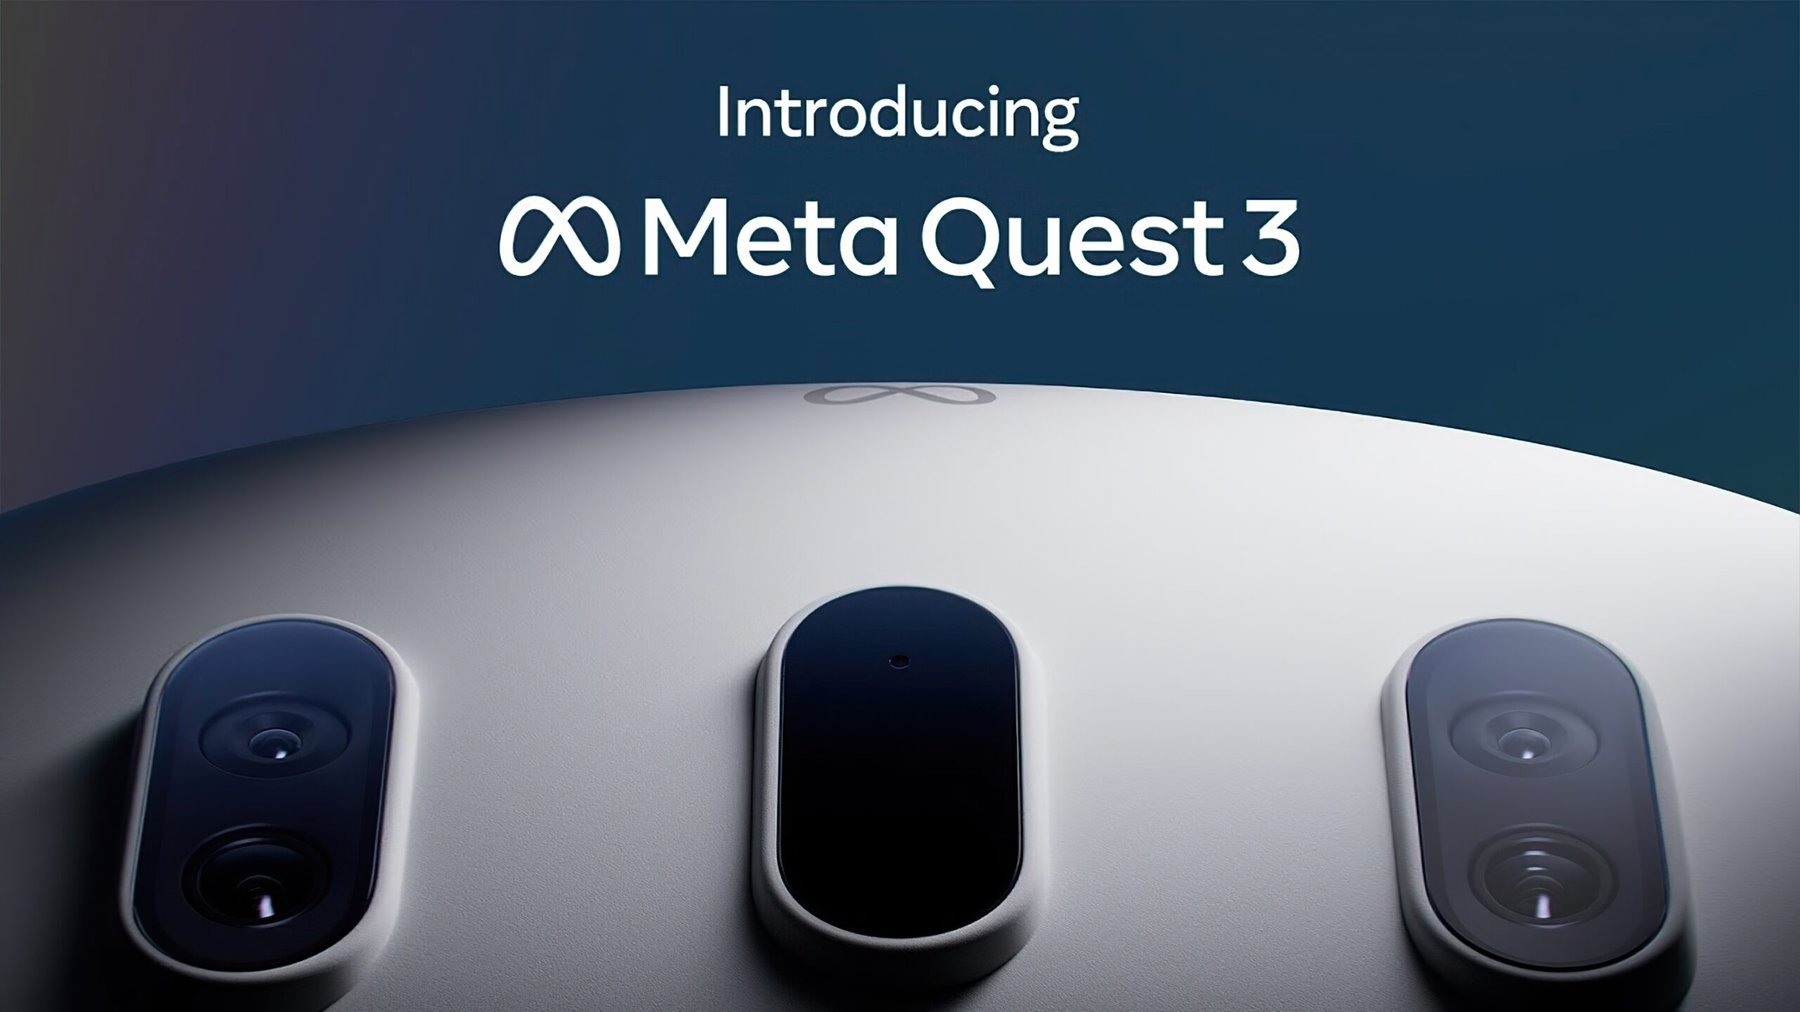
\includegraphics[width=1\textwidth]{Images/Methodologies/meta_quest_3.jpg}
    \caption{Kính thực tế ảo Meta Quest 3}
\end{figure}

Meta Quest 3 là một kính thực tế ảo/ thực tế tăng cường độc lập (standalone VR/MR), là phiên bản mới nhất trong chuỗi thiết bị thực tế ảo được sản xuất bởi Meta. Meta Quest 3 được thiết kế như một thiết bị thực tế ảo nhỏ gọn nhưng mạnh mẽ, cung cấp trải nghiệm tuyệt vời cho người sử dụng thông thường với mức giá hợp lý. Về hiệu năng, Meta Quest 3 trang bị cho mình chip Snapdragon XR2 Gen 2, đem lại gấp đôi hiệu năng xử lý đồ họa, giúp tăng đáng kể thời gian tải ứng dụng và đem lại trải nghiệm mượt mà hơn nhiều so với phiên bản tiền nhiệm Oculus Quest 2. 

Về dung lượng bộ nhớ, Meta Quest 3 sở hữu bộ nhớ mặc định là 512GB, cho phép người dùng có thể thoải mái lưu trữ các tài nguyên, phần mềm và video ưa thích. Ngoài ra, điểm nổi bật của phiển bản Quest 3 hiện tại là khả năng nhìn xuyên kính (passthrough). Với vai trò là một kính thực tế ảo (VR) kiêm thực tế tăng cường (XR), Quest 3 cho phép người dùng đang đeo kính có thể thấy được không gian bên ngoài rõ ràng, một cải tiến tuyệt vời so với phiên bản Oculus 2. 

Ngoài ra, với âm thanh 3D tích hợp trong kính cùng với lượng RAM 8GB, đem lại hiệu năng cao và phù hợp để trải nghiệm mọi ứng dụng ưa thích.

\section{Unity Engine}

Unity là một \textbf{game engine} và nền tảng phát triển ứng dụng đa nền tảng được phát triển bởi Unity Technologies, ra đời từ năm 2005 và hiện là một trong những engine được sử dụng rộng rãi nhất thế giới không chỉ trong lĩnh vực game mà còn trong mô phỏng, đào tạo, kiến trúc, y tế và robot học. Unity hỗ trợ xuất bản ứng dụng trên hơn 20 nền tảng khác nhau, bao gồm PC, Android, iOS, WebGL, và đặc biệt là các thiết bị thực tế ảo (VR) như Meta Quest, HTC Vive, PlayStation VR.

\begin{figure}[H]
    \centering
    
\includegraphics[width=0.8\textwidth]{Images/Methodologies/unity_logo.jpg}
    \caption{Unity Engine}
    \label{fig:unity_logo}
\end{figure}

\textbf{Kiến trúc cơ bản của Unity}

Unity sử dụng mô hình lập trình hướng thành phần (Component-Based Architecture), trong đó mọi đối tượng trong cảnh (scene) đều là một \lstinline[style=inlinecode]{GameObject}. Tính năng và hành vi của đối tượng được xác định bởi các \lstinline[style=inlinecode]{Component} gắn vào nó - ví dụ: \lstinline[style=inlinecode]{Transform} (vị trí, góc xoay, tỷ lệ), \lstinline[style=inlinecode]{Renderer} (hiển thị hình ảnh), \lstinline[style=inlinecode]{Collider} (va chạm vật lý), hay các script C\# tùy biến. Ngôn ngữ lập trình chính thức duy nhất của Unity là \textbf{C\#}, cho phép lập trình viên viết logic, xử lý sự kiện và tương tác với toàn bộ API của engine.

\textbf{Hỗ trợ phát triển VR/MR với Meta SDK}

Để phát triển ứng dụng thực tế ảo cho thiết bị Meta Quest 3, Unity tích hợp trực tiếp với \textbf{Meta XR SDK} (trước đây là Oculus Integration). SDK này cung cấp:

\begin{itemize}
    \item Các \lstinline[style=inlinecode]{Prefab} và component sẵn có cho camera VR, tay cầm (controllers) và tính năng passthrough (xem xuyên kính).
    \item Hệ thống \textbf{XR Interaction Toolkit} hỗ trợ các tương tác tay cầm như grab (cầm nắm), poke (chạm), teleport (dịch chuyển).
    \item Tích hợp với hệ thống \textbf{OVRInput} để đọc trạng thái các nút bấm, joystick và cảm biến tay cầm một cách đơn giản.
    \item Hỗ trợ \textbf{hand tracking} nhận dạng và theo dõi cử chỉ bàn tay người dùng mà không cần tay cầm.
\end{itemize}

\textbf{Vai trò của Unity trong đề tài}

Trong đề tài này, Unity Engine được sử dụng để xây dựng \textbf{ứng dụng VR điều khiển cánh tay robot từ xa}. Ứng dụng kết nối với hệ thống ROS2 thông qua thư viện ROS-Sharp và giao thức WebSocket của RosBridge, cho phép người dùng đeo kính Meta Quest 3 để:

\begin{itemize}
    \item Theo dõi trạng thái cánh tay robot thực tế theo thời gian thực thông qua mô hình 3D đồng bộ.
    \item Xem hình ảnh camera từ môi trường làm việc của robot.
    \item Điều khiển cánh tay bằng tay cầm VR với chế độ real-time servoing.
    \item Lập kế hoạch và thực thi quỹ đạo di chuyển qua giao diện tương tác trực quan.
    \item Điều khiển đóng/mở tay gắp.
\end{itemize}

\section{ROS-Sharp (ROS\#)}

ROS-Sharp (hay ROS\#) là một thư viện mã nguồn mở được phát triển bởi Siemens AG, cung cấp khả năng \textbf{giao tiếp hai chiều giữa Unity và hệ thống ROS/ROS2} thông qua giao thức \textbf{WebSocket} và chuẩn \textbf{ROSBridge Protocol}. Thư viện này cho phép các ứng dụng Unity subscribe và publish các ROS topic, gọi các ROS service và gửi/nhận Action goals mà hoàn toàn không cần cài đặt ROS trực tiếp trên máy chạy Unity.

\begin{figure}[H]
    \centering
    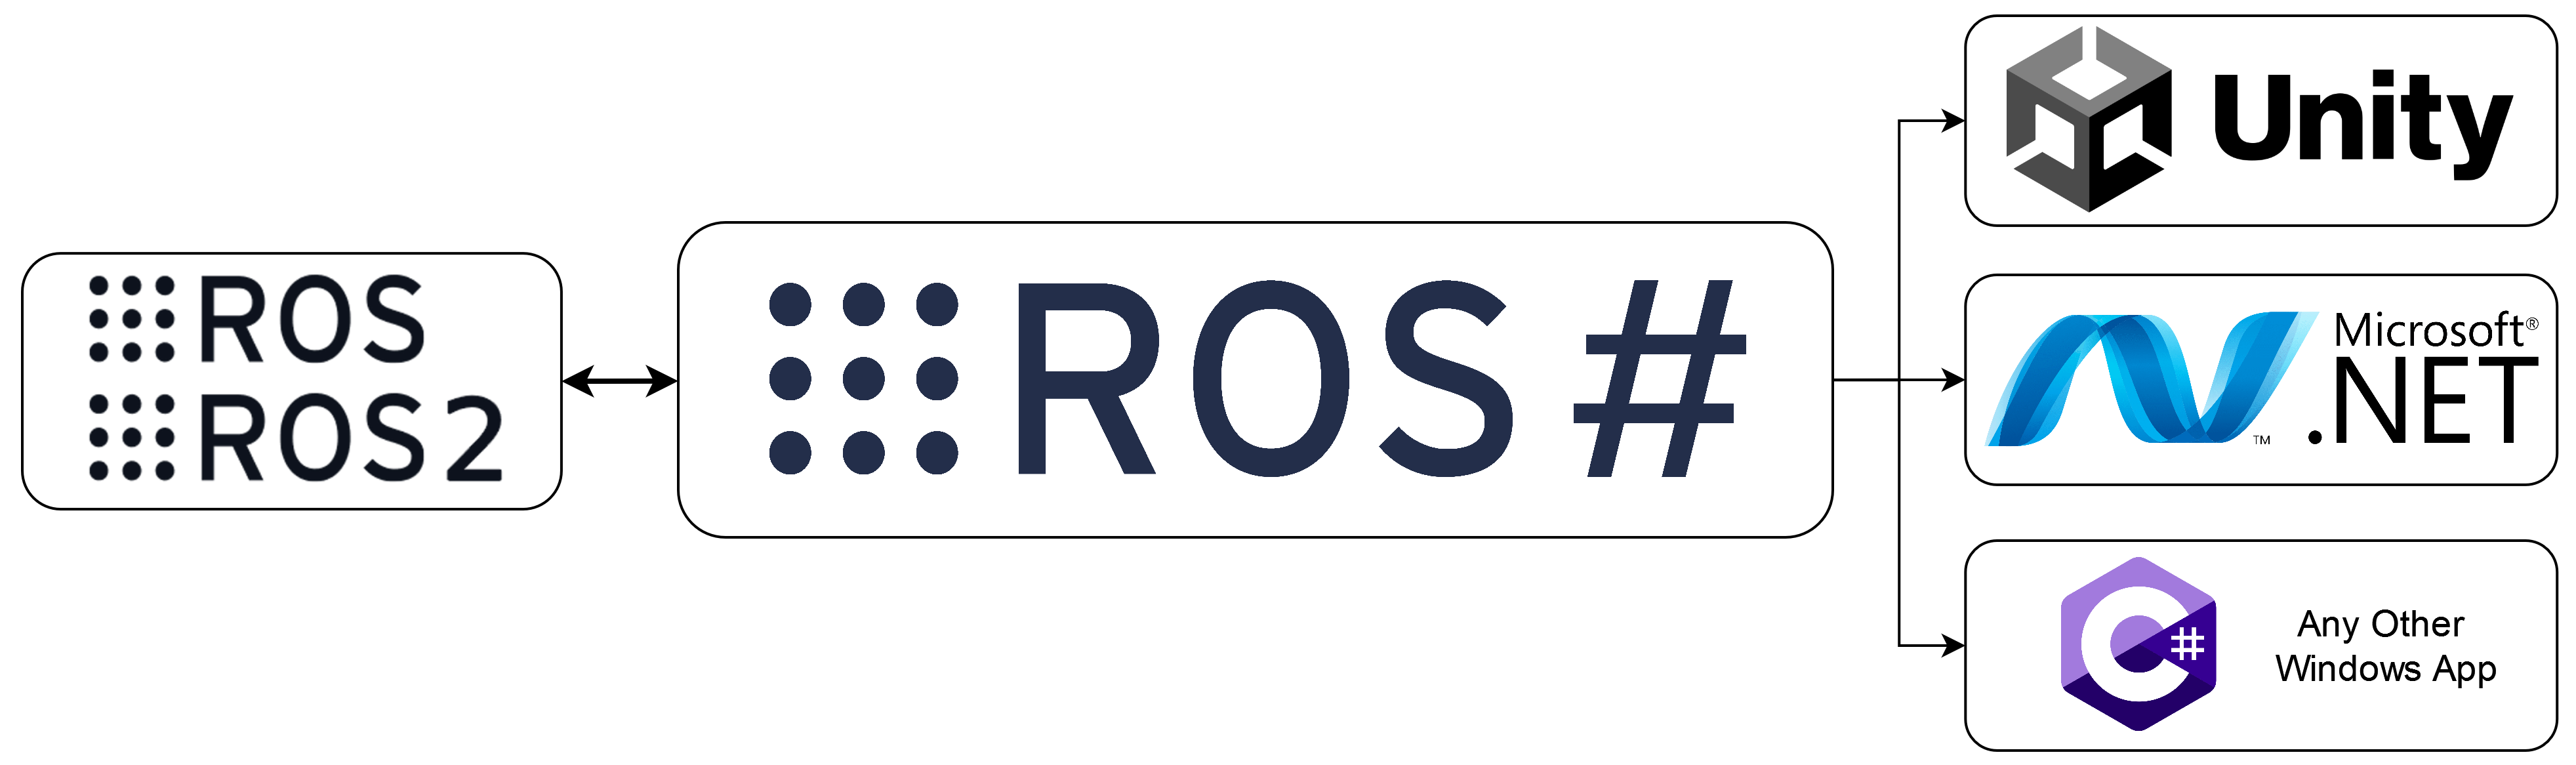
\includegraphics[width=0.8\textwidth]{Images/Methodologies/rossharp_architecture.png}
    \caption{Kiến trúc giao tiếp của ROS-Sharp giữa Unity và ROS2}
    \label{fig:rossharp}
\end{figure}

\textbf{Kiến trúc hoạt động}

ROS-Sharp hoạt động theo mô hình client-server:

\begin{itemize}
    \item \textbf{Phía ROS2 (Server)}: \lstinline[style=inlinecode]{rosbridge_server} lắng nghe kết nối WebSocket tại cổng mạng được cấu hình (mặc định 9090). Mọi thông điệp ROS2 (topic, service, action) đều được serialize sang định dạng JSON theo chuẩn \textit{rosbridge protocol v2.0}.
    \item \textbf{Phía Unity (Client)}: ROS-Sharp cung cấp class \lstinline[style=inlinecode]{RosConnector} thiết lập kết nối WebSocket tới rosbridge server. Từ đó, các script C\# có thể sử dụng các class \lstinline[style=inlinecode]{Subscriber<T>}, \lstinline[style=inlinecode]{Publisher<T>}, \lstinline[style=inlinecode]{ServiceProvider<TReq, TResp>} để tương tác với bất kỳ kênh giao tiếp ROS2 nào.
\end{itemize}

\textbf{Các tính năng chính của ROS-Sharp}

\begin{itemize}
    \item \textbf{Topic Communication}: Publish và subscribe các ROS2 topic với kiểu dữ liệu tương ứng (ví dụ: \lstinline[style=inlinecode]{JointState}, \lstinline[style=inlinecode]{TwistStamped}, \lstinline[style=inlinecode]{Image}). ROS-Sharp tự động serialize/deserialize JSON thành các đối tượng C\# tương ứng.
    \item \textbf{Service Call}: Gọi các ROS2 service từ Unity và nhận kết quả phản hồi không đồng bộ.
    \item \textbf{Action Goal}: Gửi Action goal và nhận Feedback, Result của ROS2 Action thông qua WebSocket.
    \item \textbf{URDF Importer}: Một tính năng quan trọng của ROS-Sharp là khả năng \textbf{import mô hình robot từ URDF} trực tiếp vào Unity. Kết hợp với \lstinline[style=inlinecode]{file_server} package phía ROS2, Unity có thể tải toàn bộ file URDF cùng các file mesh (\lstinline[style=inlinecode]{.dae}, \lstinline[style=inlinecode]{.stl}) về và dựng lại mô hình 3D đầy đủ của robot trong scene VR.
\end{itemize}

\textbf{Vai trò trong đề tài}

Trong đề tài, ROS-Sharp là cầu nối thiết yếu giúp ứng dụng Unity VR kết nối với toàn bộ stack điều khiển ROS2 đã xây dựng. Cụ thể, các kênh giao tiếp được sử dụng bao gồm:

\begin{itemize}
    \item Subscribe topic \lstinline[style=inlinecode]{/joint_states} để cập nhật liên tục trạng thái góc xoay của cánh tay, đồng bộ mô hình 3D trong VR với robot thực tế.
    \item Subscribe topic \lstinline[style=inlinecode]{/image_raw} (hoặc topic camera tương ứng) để hiển thị luồng video từ camera gắn trên robot.
    \item Gửi Action goal tới \lstinline[style=inlinecode]{move_to_pose} (module Denso Remote Control) để lập kế hoạch và thực thi quỹ đạo di chuyển.
    \item Gọi service \lstinline[style=inlinecode]{~/start_servo} / \lstinline[style=inlinecode]{~/stop_servo} để bật/tắt chế độ MoveIt Servo.
    \item Publish topic \lstinline[style=inlinecode]{~/delta_joint_cmds} hoặc \lstinline[style=inlinecode]{~/delta_twist_cmds} để gửi lệnh điều khiển real-time trong chế độ Servo.
    \item Gửi Action goal tới \lstinline[style=inlinecode]{gripper_cmd} (denso\_hand\_controller) để điều khiển đóng/mở tay gắp.
\end{itemize}

Nhờ ROS-Sharp và rosbridge\_server, toàn bộ logic điều khiển phức tạp nằm ở phía ROS2, còn Unity chỉ cần đảm nhiệm phần giao diện người dùng và trải nghiệm VR, tạo ra sự phân tách rõ ràng và linh hoạt trong kiến trúc hệ thống.

\chapter{THIẾT KẾ VÀ HIỆN THỰC HỆ THỐNG}

\section{Sơ đồ thiết kế hệ thống}

Sơ đồ thiết kế của hệ thống điều khiển cánh tay robot Denso được trình bày ở hình dưới:

\begin{figure}[H]
    \centering
    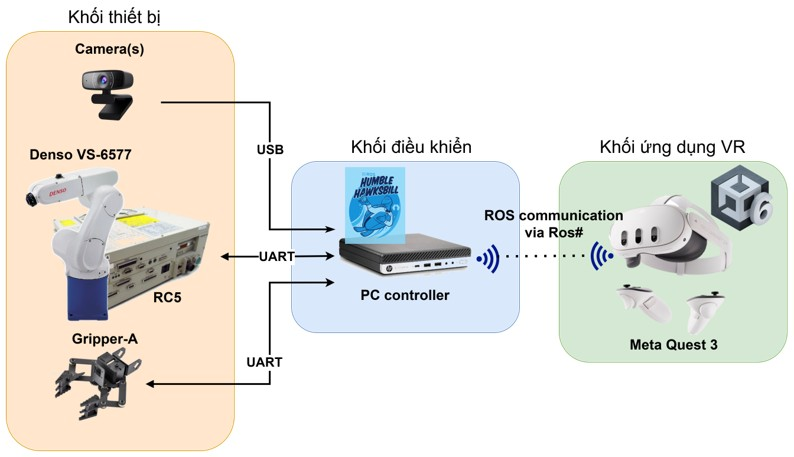
\includegraphics[width=1\linewidth]{Images/Implementation/System_architecture.jpg}
    \caption{Sơ đồ thiết kế của hệ thống điều khiển}
    \label{fig:placeholder}
\end{figure}

Trong sơ đồ này, có các khối chức năng chính có thể kể đến như:

\begin{itemize}
    \item \textbf{Cánh tay robot Denso VS-6577E}: 
    
    Đây là thiết bị điều khiển chính trong dự án, với 6 trục tự do, cánh tay có độ linh hoạt và ổn định cao, phù hợp cho các công việc đòi hỏi sự chỉnh xác, kể cả trong môi trường công nghiệp
    \item \textbf{Máy điều khiển RC5}:

    Đây là một máy điều khiển robot hiệu năng cao, RC5 đóng vai trò quan trọng để trực tiếp điều khiển các trục của cánh tay robot Denso thông qua các dây kết nối ở cổng CN12. Điều này cũng đồng nghĩa là để có thể xoay các trục cánh tay, ta cần phải tận dụng RC5. Như đã trình bày ở Chương 2, ngoài khả năng điều khiển trực tiếp bằng teach pendant, RC5 cũng cho phép người dùng viết "PAC script" - là một ngôn ngữ lập trình chuyên biệt cho thiết bị để điều khiển từ nhà sản xuất Denso. Qua việc thiết kế các PAC script, nhóm hiện thực khả năng nhận lệnh điều khiển cánh tay robot thông qua lệnh UART, đẩy các tính năng chính và lớn lên module tiếp theo: PC Controller.
    \item \textbf{PC Controller}: 

    PC Controller đóng vai trò là bộ điều khiển trung tâm, là cầu nối giữa thiết bị điều khiển thông dụng khác với cụm RC5-Cánh tay VS-6577E. Trên PC Controller sẽ được tập trung phát triển các cơ chế điều khiển cánh tay cũng như cập nhật trạng thái cánh tay tận dụng ROS2. ROS2 đem lại cho nhà phát triển một hệ sinh thái đa dạng, mạnh mẽ, giúp nhà phát triển có thể dễ dàng triển khai các ứng dụng robot đa dạng, phức tạp mà không bị phụ thuộc bởi máy RC5 của Denso. Nhóm tập trung xây dựng một cơ chế giao tiếp hiệu quả, tốc độ cao và đáng tin cậy giữa thiết bị điều khiển bên ngoài và cánh tay robot Denso, từ đó tạo nền móng cho việc phát triển nhiều ứng dụng trên cánh tay robot sau này.

    \item \textbf{Các camera}:

    Như đã trình bày ở các phần trên và quan sát cả các nghiên cứu liên quan, Camera là một thành phần không thể thiếu trong kiến trúc hệ thống, với vai trò quan trọng là mang lại phản hồi hình ảnh thực tế về môi trường xung quanh và chính cánh tay robot được điều khiển ở xa, qua đó tăng cường trải nghiệm vận hành, điều khiển, giúp tăng hiệu suất điều khiển từ xa hơn so với các phương pháp truyền thống.

    \item \textbf{Meta Quest 3}

    Meta Quest 3 được nhóm lựa chọn là thiết bị VR sẽ được sử dụng trong đồ án. Một ứng dụng VR sẽ được phát triển tận dụng Unity Engine và thư viện VR được cung cấp và phát triển bởi Meta, với mục tiêu xây dựng ứng dụng điều khiển, tương tác hiệu quả, trực quan, đồng bộ tốt với cánh tay thực tế. Việc cho phép người dùng sử dụng VR để điều khiển cánh tay sẽ đem lại trải nghiệm sinh động, trực quan, tăng hiệu quả điều khiển cho người dùng từ xa mà không đánh đổi sự tiện lợi, cung cấp đầy đủ các tính năng điều khiển thông dụng như trên thiết bị truyền thống.
\end{itemize}

Các phần tiếp theo lần lượt trình bày phương thức hiện thực các module chính đã được mô tả phía trên.

\section{Xây dựng chương trình điều khiển cánh tay bằng RC5}

\subsection{Thiết kế chương trình}

Trong giai đoạn một, chương trình trên RC5 dù đơn giản, nhưng lại có nhiều điểm yếu như sau:
\begin{itemize}
    \item Chương trình phụ thuộc vào hàm nhận và tách dữ liệu UART tự động của RC5, tuy nhiên hàm lại không hỗ trợ cơ chế nhận diện và xử lý khi chuỗi nhận bị lỗi. Khi bị lỗi, chương trình bị dừng hoàn toàn và phải khởi động lại một cách thủ công
    \item Chu trình hoạt động không liên tục: Luồng chạy yêu cầu phải nhận dữ liệu, xử lý, xong mới xoay cánh tay robot. Điều này tạo ra điểm ngắt quãng giữa các lệnh xoay, khiến cho robot xoay bị giật và không mượt mà
    \item Hàm xoay robot "Move" tốn nhiều thời gian tính toán thay vì dùng các lệnh xoay trực tiếp trục như "DriveA"
\end{itemize}

Ở giai đoạn này, chương trình đã được nâng cấp đáng kế để giải quyết hai điểm yếu lớn trên, cụ thể:

\begin{itemize}
    \item Phân tách chương trình gốc thành 4 chương trình con khác nhau, mỗi chương trình đảm nhiệm một nhiệm vụ cụ thể:
    \begin{itemize}
        \item \lstinline[style=inlinecode]{GET_JOINT.pac}: Đọc giá trị các trục hiện tại của Robot và gửi giá trị đó qua UART
        \item \lstinline[style=inlinecode]{task0.pac}: Đọc lệnh UART từ PC Controller gửi xuống và lưu vào buffer.
        \item \lstinline[style=inlinecode]{TASK1CRC.pac}: Khi có giá trị buffer mới, tiến hành xử lý dữ liệu đó dưới dạng string để giải mã lệnh điều khiển, và lưu vào một Ring Buffer
        \item \lstinline[style=inlinecode]{task3.pac}: Đọc lệnh điều khiển từ Ring Buffer và xoay cánh tay robot tương ứng
    \end{itemize}
    \item Sử dụng cơ chế chạy đồng thời: ngôn ngữ PAC trên RC5 cho phép chạy các đoạn chương trình một cách đồng thời theo chu kì thời gian định trước. 
    \item Viết chương trình riêng để xử lý lệnh UART ở dạng string để có quyền kiểm soát và phát hiện lỗi
    \item Sử dụng hàm xoay từng trục trực tiếp để giảm thiểu thời gian tính toán.
\end{itemize}

Sau cùng, chương trình tổng \lstinline[style=inlinecode]{MAIN.pac} sẽ chạy bốn chương trình trên đồng thời theo chu kì, kèm theo một số khởi tạo cần thiết cho hoạt động của cánh tay robot.

\begin{lstlisting}
'!TITLE "MAIN"
PROGRAM MAIN
    DEFIN li1
    REM ========= I1 notify that new string data is received. after processed, set I1 to 0 to wait for new data.
    I1 = 0
    REM ========= I4 and I5 used for ring buffer for processed joint.
    I4 = 0
    I5 = 0
    FLUSH #1
    FOR li1 = 0 to 99
        J[li1] = (0,0,0,0,0,0)
    NEXT li1
    REM ==== Read Serial Task
    RUN TASK0, C = 10
    DELAY 20
    REM ==== Process recevied data
    RUN TASK1CRC, C = 15
    REM ==== RUN ROBOT
    RUN TASK3, C = 35
    REM ==== Transmit current joint
    RUN GET_JOINT, C = 100
END
\end{lstlisting}

Phần tiếp theo trình bày chi tiết cơ chế hoạt động của chương trình tại RC5.

\subsection{Cơ chế nhận lệnh, xử lý lệnh kiểu chuỗi và xoay cánh tay robot}

Đây chính là cơ chế quan trọng nhất trong chuỗi lệnh điều khiển của RC5, chính vì vậy nó được thiết kế để đảm bảo các tiêu chí: hoạt động ổn định, nhanh, mượt mà và có khả năng chịu lỗi để có thể chạy liên tục trong thời gian dài. Kiến trúc hoạt động của chương trình được thể hiện bên dưới:

\begin{figure}[H]
    \centering
    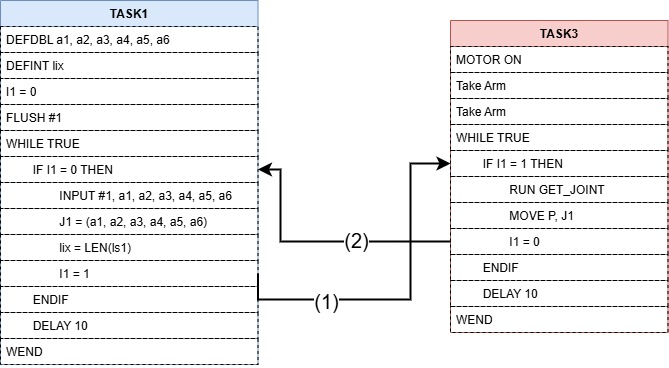
\includegraphics[width=0.8\linewidth]{Images/Implementation/Control/RC5_software.jpg}
    \caption{Kiến trúc chương trình điều khiển RC5}
    \label{fig:rc5-program-architecture}
\end{figure}

Chương trình MAIN.pac có vai trò khởi chạy các chương trình con theo chu kì phù hợp, trong đó:
\begin{itemize}
    \item \textbf{TASK0}: dùng để đọc lệnh Serial, do đó cần chạy liên tục và nhanh với chu kì 10ms. Lệnh UART sẽ được rút ra từ buffer UART nội bộ của máy RC5, chỉ khi có dữ liệu serial và cờ đọc sẵn sàng (\lstinline[style=inlinecode]{I1 = 0}). Dữ liệu UART được đọc và lưu trữ vào biến chuỗi toàn cục \lstinline[style=inlinecode]{S1}, cờ đọc bị chặn (\lstinline[style=inlinecode]{I1 = 1}) để cho phép code xử lý chuỗi bắt đầu chạy ở \textbf{TASK1CRC}
    \item \textbf{TASK1CRC:} Khi cờ \lstinline[style=inlinecode]{I1 = 1}, chương trình xử lý chuỗi sẽ lấy dữ liệu lưu trong \lstinline[style=inlinecode]{S1} và bắt đầu nhiệm vụ phân tách. Format của lệnh điều khiển ở dạng như sau:
    \begin{lstlisting}[language={}]
    J1,J2,J3,J4,J5,J6#LEN_PAYLOAD
\end{lstlisting}
    Trong đó, \lstinline[style=inlinecode]{J[X]} lần lượt là giá trị góc (tính theo độ) của từng trục, giá trị này cần ở dạng số nguyên có dấu. Trên thực tế, robot hoàn toàn có thể được điều khiển với giá trị góc là số thực (có dấu chấm động), tuy nhiên, việc xử lý chuỗi có dấu chấm động tăng tính phức tạp và thời gian chạy của hàm xử lý chuỗi, do đó giá trị góc dạng số thực sẽ sẽ được gửi xuống UART ở dạng \lstinline[style=inlinecode]{angle * 100}, và chia ngược lại ở RC5 

    Ngoài ra, format lệnh còn có thêm \lstinline[style=inlinecode]{LEN_PAYLOAD}, được phân cách bởi ký tự đặc biệt "\#", dùng để chứa độ dài của chuỗi lệnh trước dấu "\#". Lý do là vì trong quá trình phát triển, giao tiếp giữa RC5 và PC controller thường gặp trục trặc, chủ yếu là do dữ liệu UART truyền tới RC5 bị mất hoặc dư kí tự, từ đó tạo giá trị góc sai lệch hoặc lỗi trong lúc giải mã chuỗi. Chính vì vậy, việc sử dụng \lstinline[style=inlinecode]{LEN_PAYLOAD} có tác dụng như một cơ chế kiểm tra toàn vẹn dữ liệu đơn giản, giúp chương trình xử lý chuỗi có thể phát hiện sớm chuỗi bị lỗi và loại bỏ, đảm bảo khả năng hoạt động ổn định trong thời gian dài ở phía cánh tay robot. Khối CRC\_check ở sơ đồ trên thể hiện tính năng này, trong đó chuỗi được xem là lỗi khi:
    \begin{enumerate}
        \item Không tìm thấy dấu "\#"
        \item Tìm thấy dấu "\#", nhưng \lstinline[style=inlinecode]{LEN_PAYLOAD} khác với độ dài của chuỗi nhận được bên trái dấu "\#".
    \end{enumerate}

    Chuỗi dữ liệu hợp lệ (pass được khối CRC\_check) sẽ tiến tới phần bóc tách dữ liệu góc joint\_seperation, qua đó từng giá trị số nguyên sẽ được lấy ra, convert sang giá trị số và chia 100 để lấy giá trị số thực của góc xoay. Sáu giá trị góc sau đó lưu vào biến toàn cục \lstinline[style=inlinecode]{J[I5]}. \lstinline[style=inlinecode]{I5 + 1} và \lstinline[style=inlinecode]{I1 = 0} để cho phép \textbf{TASK0} đọc vào chuỗi UART tiếp theo.
    \item \textbf{TASK3:} Chương trình được cải tiến để tránh khoảng ngừng giữa các lần xoay bằng cơ chế Ring Buffer. Cụ thể, trong RC5 cho phép người dùng sử dụng các biến toàn cục, trong đó \lstinline[style=inlinecode]{J[X]}, với X từ 0 -> 99 là 100 biến toàn cục dùng để chứa giá trị góc (joint). Hai biến toàn cục \lstinline[style=inlinecode]{I4, I5} được sử dụng, trong đó 
    \begin{enumerate}
        \item \lstinline[style=inlinecode]{I5} thể hiện lệnh xoay joint \textbf{trong tương lại}, liên tục tăng mỗi khi chuỗi được xử lý xong ở \textbf{TASK1CRC} và giá trị góc được lưu vào \lstinline[style=inlinecode]{J[I5]}
        \item Ở \textbf{TASK3}, \lstinline[style=inlinecode]{I4} thể hiện lệnh xoay joint \textbf{đã xử lý}, nếu \lstinline[style=inlinecode]{I4 < I5} tức là vẫn còn lệnh chưa được xử lý, \lstinline[style=inlinecode]{J[I4]} sẽ được dùng để xoay các trục robot, sau đó tăng \lstinline[style=inlinecode]{I4 + 1} cho tới khi đuổi kịp \lstinline[style=inlinecode]{I5}
    \end{enumerate}
    Cơ chế này đem lại sự linh hoạt và giảm đáng kể các khoảng ngừng giữa các lệnh xoay, bởi I5 thì cứ tăng (chuỗi được xử lý liên tục), trong khi ở \textbf{TASK3}, I4 cũng liên tục đuổi theo I5 và xoay các trục của cánh tay theo chuỗi lệnh. I5 chắc chắn sẽ chạy nhanh hơn I4, nên \textbf{TASK3} cũng sẽ liên tục có các giá trị góc xoay mới mà không bị ngắt giữa chừng.
\end{itemize}

\subsection{Cơ chế cập nhật trạng thái robot}

So với cơ chế điều khiển, cơ chế cập nhật trạng thái của robot có phần đơn giản hơn hơn nhờ sự hỗ trợ trực tiếp từ RC5. Chương trình \textbf{GET\_JOINT} liên tục lấy giá trị góc của 6 trục robot thông qua \lstinline[style=inlinecode]{CURJNT} và gửi lên PC Controller mỗi 100ms với format:

\begin{lstlisting}[language={}]
    j1, j2, j3, j4, j5, j6\r
\end{lstlisting}

So với lệnh điều khiển, lệnh cập nhật trạng thái có phần ổn định và ít lỗi hơn, do đó cơ chế CRC hiện chưa cần thiết. Thêm nữa, ở phía PC controller đã có nhiều đoạn code xử lý và phát hiện lỗi ở nhiều cấp độ: cấp UART, cấp Driver và cấp Hardware Interface, đủ để loại bỏ các chuỗi trạng thái lỗi mà vẫn đảm bảo chương trình hoạt động ổn định trong thời gian dài.

\section{Kiến trúc phần mềm điều khiển bằng ROS2}

Kèm theo với nhiều cải tiến trong code xử lý lệnh ở RC5, độ ổn định giữa giao tiếp RC5 - PC controller tạo tiền đề để phát triển, mở rộng hơn kiến trúc phần mềm ROS2 đã có ở giai đoạn một. Tiêu chí thiết kế vẫn tương tự ở giai đoạn hai, phần hiện thực sẽ trở nên phức tạp hơn đối với tầng điều khiển ở PC Controller. ROS2 được sử dụng làm nền tảng để xây dựng cơ chế điều khiển robot, với nhiều công cụ hỗ trợ và mạnh mẽ nhằm tăng tốc khả năng hiện thực. Hơn nữa, đề tài chủ trương xây dựng chương trình Ros2 sử dụng ngôn ngữ C++ thay vì python và ROS1, với mục tiêu là sử dụng những công nghệ mới nhất trong lập trình robot, cũng như tạo cơ hội để tiếp cận những bộ công cụ hiện đại hơn. Về phiên bản ROS2, đề tài sử dụng ROS2 Humble trong Ubuntu 22.04, do sự phổ biến của nó trong cộng đồng phát triển cũng như được hỗ trợ rộng rãi bởi nhiều bộ công cụ bên thứ ba. Kết hợp với ROS2, đề tài sử dụng thêm Ros2-Control và ROS2-Moveit, nhanh chóng tạo dựng cơ chế điều khiển cánh tay robot theo tiêu chuẩn của những dự án ROS2 đã được xây dựng và nghiên cứu trước đó.

Hiện thực ROS2 của đồ án có thể tìm thấy ở đây: \href{https://github.com/ngoccatt/ros2_arctos_HCMUT}{ros2\_arctos\_HCMUT}

\subsection{Sơ đồ kiến trúc phần mềm dựa trên Ros2-Control}

\begin{figure}[H]
    \centering
    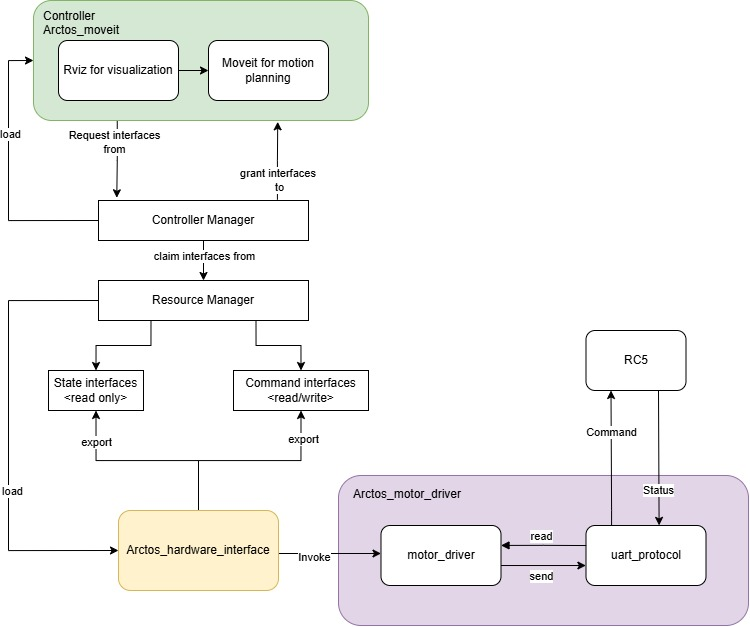
\includegraphics[width=0.8\linewidth]{Images/Implementation/Control/ros2_control.jpg}
    \caption{Sơ đồ kiến trúc phần mềm dựa trên Ros2-Control}
    \label{fig:placeholder}
\end{figure}

Đề tài chủ trương xây dựng chương trình điều khiển cánh tay robot VS-6577E theo kiến trúc của Ros2-Control, bao gồm các khối như controller, hardware interface và driver. Xây dựng phần mềm theo kiến trúc của Ros2-Control đem lại những ưu điểm như

\begin{itemize}
    \item Module hóa các lớp điều khiển, giúp dễ kiểm soát, bảo trì và kiểm thử.
    \item Tạo khả năng mở rộng và dùng lại tốt, có thể dễ dàng điều chỉnh để thay thế phần driver hoặc hardware interface sử dụng cho robot khác, trong khi phần controller và lớp ứng dụng cao hơn được giữ nguyên.
    \item ROS2-Control sử dụng cơ chế hoạt động theo chu kì \textbf{update-write-read} đơn giản nhưng mạnh mẽ, là nền tảng để xây dựng chương trình vận hành robot thời gian thực
    \item Tích hợp dễ dàng với MoveIt để xử lý việc điều khiển và lập kế hoạch quỹ đạo cánh tay với các giải thuật động học hiệu quả
\end{itemize}

Phần tiếp theo mô tả các khối chính trong mô hình kiến trúc theo Ros2-control mà đề tài vận dụng.

\subsection{Khối Driver}

Khối Driver là tầng dưới cùng trong kiến trúc Ros2-Control, có vai trò giao tiếp trực tiếp với phần cứng - cánh tay robot VS-6577E thông qua máy điều khiển RC5 và tay gắp Gripper-A thông qua Driver-Hat-A. Cả hai bộ điều khiển trung gian: RC5 và Driver-Hat-A đều hỗ trợ giao thức UART, do đó khối \lstinline[style=inlinecode]{UartProtocol} có thể được tái sử dụng ở cả hai phía. Tuy nhiên, mỗi driver sẽ khởi tạo một đối tượng \lstinline[style=inlinecode]{UartProtocol} riêng để đảm bảo quá trình truyền nhận dữ liệu tách biệt và không xung đột.

\subsubsection{Khối UartProtocol} 

Khối UartProtocol được xây dựng các chức năng để hỗ trợ truyền/nhận dữ liệu UART, phân tích dữ liệu theo định dạng đã đề xuất và lưu trữ dữ liệu nhận được để tránh mất gói tin. Một số tính năng của module này có thể kể tới như:
\begin{itemize}
    \item \textbf{Thiết kế class}: Uart\_protocol có thể được khởi tạo như một object riêng biệt ở mỗi module khác cần sử dụng, giúp tách biệt luồng dữ liệu và tránh xung đột khi tạo nhiều giao tiếp UART.
    
    \item \textbf{Cơ chế lưu dữ liệu nhanh chóng}: Khi có dữ liệu mới, module này sẽ nhanh chóng lưu nó vào một buffer riêng, và khi cần sẽ lấy dữ liệu ra theo FIFO. Để đáp ứng cơ chế này, module sử dụng UART cần gọi hàm \lstinline[style=inlinecode]{readToBuffer()} liên tục trong một thread riêng, và gọi \lstinline[style=inlinecode]{getFromBuffer()} để lôi dữ liệu ra ngoài khi cần.
    
    \item \textbf{Hàm hỗ trợ truyền dữ liệu cơ bản}: hai hàm \lstinline[style=inlinecode]{sendMsg()} và \lstinline[style=inlinecode]{sendMsgWithCLRF()} có thể được sử dụng để truyền một chuỗi kí tự đi tới kết nối UART.
    
    \item \textbf{Hỗ trợ riêng cho giao tiếp với RC5}: hai hàm \lstinline[style=inlinecode]{sendPosition()} và \lstinline[style=inlinecode]{decodeMessage()} hỗ trợ cách thức đơn giản hơn để truyền lệnh (có bao gồm cơ chế crc theo chiều dài chuỗi) và giải mã giá trị trục thực tế của robot.
    
\end{itemize}

\subsubsection{Motor Driver}

Phần Motor Driver được xây dựng để quản lý trạng thái và điều khiển các trục của cánh tay robot VS-6577. Module Motor driver mang đặc trưng điều khiển cụ thể, phù hợp với RC5 và VS-6577. Điểm mạnh của module này là: 
\begin{enumerate}
    \item Cung cấp khả năng quản lý các trục xoay bằng nhiều thuộc tính như tên trục, giới hạn min/max trục, góc xoay hiện tại, góc xoay yêu cầu, feedback, thời gian cập nhật/điều khiển...
    \item Cung cấp cơ chế kiểm tra nhiều lớp tính hợp lệ của dữ liệu điều khiển cũng như giá trị trạng thái trục được gửi lên từ cánh tay robot thực tế.
    \item Tiết kiệm thời gian xử lý bằng cách kiểm tra tính mới của giá trị trạng thái trước khi giải mã và xử lý.
    \item Thiết kế để dễ dàng quản lý, mở rộng và có thể áp dụng để điều khiển với số lượng trục linh động, các hàm được xây dựng phụ thuộc vào tham số mà người dùng hoàn toàn có thể điều chỉnh ở file config mà không cần phải build lại phần mềm.
\end{enumerate}

Cách thiết kế của Motor Driver cho phép mỗi trục là một đối tượng riêng biệt (\lstinline[style=inlinecode]{JointConfig}), giúp dễ dàng quản lý trạng thái và thuộc tính hiệu quả. Khi có lệnh mới, giá trị góc xoay yêu cầu được lưu ngay vào đối tượng \lstinline[style=inlinecode]{JointConfig}. Khi cần gửi dữ liệu điều khiển xuống RC5, các giá trị góc xoay yêu cầu được thu thập từ mỗi đối tượng và tạo thành một chuỗi lệnh ở dạng sau, với sự hỗ trợ của module Uart:

\begin{lstlisting}
J1,J2,J3,J4,J5,J6#LEN_PAYLOAD
\end{lstlisting}

Ngược lại, dữ liệu trạng thái trục truyền lên từ RC5 được phân tách, kiểm tra tính hợp lệ của dữ liệu và lưu ngược lại trong \lstinline[style=inlinecode]{JointConfig} tương ứng.

\subsubsection{Servo Driver}

Khối Servo Driver được thiết kế dựa trên Motor Driver, tuy nhiên được tinh gọn hơn là chỉ dùng để gửi lệnh tới một Servo. Mục tiêu của module này là giao tiếp với Driver-Hat-A để điều khiển tay gắp Gripper-A, và hiện Driver-Hat-A cũng chỉ hỗ trợ điều khiển một servo duy nhất, nên Servo Driver chỉ đặt thêm một ràng buộc không cho tạo nhiều hơn 1 đối tượng \lstinline[style=inlinecode]{JointConfig}. Một lý do nữa cần phải phân tách ra so với khối Motor Driver, đó là giao tiếp với Driver-Hat-A có format quy định tương đối khác so với RC5. Cụ thể, lệnh cần được gửi ở dạng JSON format. Đề tài sử dụng thư viện \href{https://github.com/nlohmann/json}{JSON for Modern C++} để có thể nhanh chóng tạo và xử lý chuỗi ở dạng JSON. Lệnh điều khiển có dạng như sau:

\begin{lstlisting}[language=json]
{"T":121,"angle":0.67,"spd":100,"acc":10}
\end{lstlisting}

Trong đó "T":121 ám chỉ đây là lệnh điều khiển, (angle) là giá trị góc xoay (radian) mà servo cần đạt tới để đóng hay mở tay gắp, với tốc độ (spd) từ 0 -> 4096 và gia tốc (acc) từ 0 -> 254. Giá trị 0 ở spd và acc yêu cầu xoay với tốc độ cao nhất.

Để lấy trạng thái góc xoay hiện tại của gripper, ta cần phải gửi lệnh JSON xuống thiết bị, thay vì thiết bị gửi trạng thái liên tục. Định dạng của lệnh là:

\begin{lstlisting}[language=json]
{"T":105}
\end{lstlisting}

Driver-hat-A sẽ phản hồi lại góc xoay, cùng nhiều thông tin khác của tay gắp ở dạng:

\begin{lstlisting}[language=json]
{"T":1051,"pos":3138,"speed":0,"load":-104,"voltage":124,"current":4,"temper":45,"mode":0}
\end{lstlisting}

Trong đó, thông tin về góc xoay hiện tại (pos) được chú trọng, tuy nhiên đây không hẳn là giá trị góc ở đơn vị "độ", mà nó là vị trí của step encoder. Ta cần phải thực hiện tính toán sau để chuyển sang giá trị độ:

\begin{align*}
angle\_deg = (pos - 1024) * (360/4096)
\end{align*}

Thêm nữa, trong quá trình xoay, lệnh đọc trạng thái có thể gửi tới Driver-Hat-A và được phản hồi ngay vị trí hiện tại của servo, cho phép module cao hơn theo dõi trạng thái xoay và góc xoay thực tế của tay gắp.

\subsection{Robot description}

Khi xây dựng ứng dụng điều khiển robot với ROS2, robot description là một module không thể thiếu. Một thư mục Robot Description thường chứa file URDF (Unified Robot Description format), dùng để định nghĩa chi tiết về cấu trúc của robot trong không gian 3D, bao gồm việc nối các bộ phận từ Mesh (một file mô tả hình dáng của cánh tay) lại với nhau và định nghĩa sự liên kết của các bộ phận đó.

Với mục tiêu mô phỏng cánh tay robot một cách chính xác nhất, đề tài chủ trương lấy chính xác mô hình 3D cùng phiên bản của cánh tay VS-6577 từ nhà sản xuất Denso. Mô hình này được import vào phần mềm SOLIDWORK 2024, sau đó thông qua plugin \href{https://github.com/ros/solidworks_urdf_exporter}{\textbf{Solidworks Urdf Exporter}} để export đặc tả URDF của cánh tay cùng các file mesh cấu thành cánh tay robot. Phần tay gắp cũng được nhóm nối trực tiếp vào trục end-effector của cánh tay, cấu thành mô hình 3D cuối cùng đang được đề tài sử dụng. 

\begin{figure}[H]
    \centering
    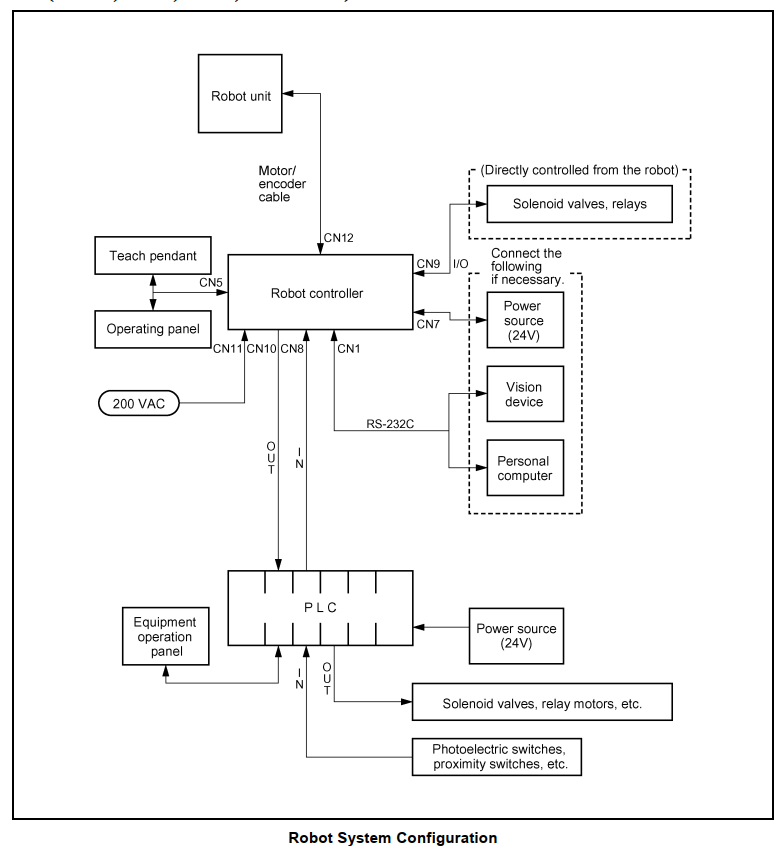
\includegraphics[width=0.85\linewidth]{Images/Implementation/Control/rc5_connection.png}
    \caption{Minh họa kết nối phần cứng phục vụ quá trình tích hợp mô hình robot}
    \label{fig:hw-connection-for-integration}
\end{figure}

Do nội dung file URDF tương đối lớn và nhiều, đề tài thực hiện phân tách thành các file ".xacro" nhỏ hơn. Xacro, hay XML Macros, là một định dạng file được dùng rộng rãi trong ROS2, cho phép lập trình viên tạo những khối đặc tả robot có thể tái sử dụng, đơn giản hóa file URDF thông qua các macro. Đặc tả robot đóng vai trò quan trọng trong việc khởi chạy Ros2-control cũng như MoveIt2, bởi các thông tin này sẽ được boardcast cho toàn mạng ROS2 và được sử dụng triệt để bởi các module để hỗ trợ việc điều khiển hiệu quả, chính xác.

\subsection{Hardware Interface}

Hardware interface là module ở tầng thứ hai trong kiến trúc Ros2-Control, có vai trò làm cầu nối trung gian giữa phần \textbf{Controller} và \textbf{Driver}. Hardware interface sẽ cung cấp các \textbf{command interface} để Controller có thể điều khiển, và \textbf{state interfaces} để cập nhật trạng thái của thiết bị thực từ Driver lên cho Controller, tuân theo thiết kế phần mềm được quy định trong Ros2-Control đối với thành phần Hardware interface. Với việc điều khiển hai thiết bị khác nhau: cánh tay VS-6577 thông qua RC5 và Gripper-A thông qua Driver-Hat-A, hệ thống cần hai hardware interface riêng biệt do cách thức hoạt động khác nhau. Trong phần hiện thực, hai lớp chính được dùng là \lstinline[style=inlinecode]{DensoInterface} cho cánh tay robot và \lstinline[style=inlinecode]{DensoHandInterface} cho tay gắp.

\subsubsection{Quá trình khởi động Hardware Interface}

Theo quy định của Ros2-Control, mọi hardware interface cần được khởi động theo một chu trình cố định, ở từng bước sẽ làm những công việc khởi tạo khác nhau để chuẩn bị kết nối với phần cứng cần điều khiển.

Sơ đồ khởi chạy của Hardware Interface được trình bày như hình dưới:

\begin{figure}[H]
    \centering
    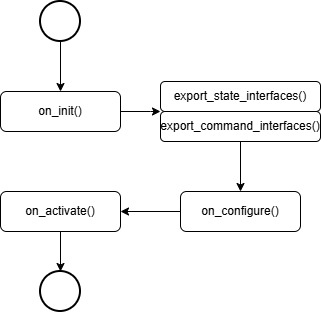
\includegraphics[width=0.5\linewidth]{Images/Implementation/Control/Init_sequence.jpg}
    \caption{Luồng khởi động của Hardware Interface}
    \label{fig:placeholder}
\end{figure}

Luồng khởi động này tuân theo tiêu chuẩn đặt ra bởi Ros2-Control, gồm bốn bước: init, export, configure và activate.

\textbf{on\_init()}

"init" là bước đầu tiên trong luồng khởi tạo. Trong bước này, dữ liệu liên quan tới cánh tay được đặc tả trong Robot Description (file urdf) dưới tag \lstinline[style=inlinecode]{<ros2_control>} sẽ được truyền vào như một tham số của hàm, hỗ trợ trong việc cung cấp thông tin khởi tạo. Một điều lưu ý là tag \lstinline[style=inlinecode]{<ros2_control>} cần chỉ rõ ở tag \lstinline[style=inlinecode]{<hardware>/<plugin>} hardware interface mà nó cần sử dụng, qua đó giúp bản thân Ros2\_Control dẫn các dữ liệu về trục hoặc param tới hardware interface tương ứng. Nhờ cơ chế này, hàm \lstinline[style=inlinecode]{on_init()}  biết được số lượng trục cánh tay robot được mô tả qua dưới tag \lstinline[style=inlinecode]{<ros2_control>}, qua đó tạo dựng các mảng dữ liệu (dạng \lstinline[style=inlinecode]{<vector>} để lưu trữ trạng thái và lệnh điều khiển. Ngoài ra, hàm \lstinline[style=inlinecode]{on_init()} cũng khai báo một số ros parameter mới như \lstinline[style=inlinecode]{motor_id, hardware_type, gear_ratio, inverted, inverted_feedback} ... để chuẩn bị cho bước \lstinline[style=inlinecode]{configure} tiếp theo.

\textbf{export\_state\_interfaces() và export\_command\_interfaces()}

Tiếp đến là bước "export" các "State interface" (dùng để cập nhật trạng thái) và "Command interface" (dùng để ghi lệnh điều khiển). Bước này có vai trò quan trọng trong cấu trúc Ros2-Control, cung cấp đủ interface cho trạng thái và điều khiển thiết bị cho Resource Manager (quản lý tài nguyên), qua đó các Controller có thể "chiếm" những interface này thông qua Controller Manager. Để tránh xung đột về việc sử dụng tài nguyên, một Command interface chỉ có thể được sở hữu bởi một controller, trong khi đó State interface có thể được sử dụng bởi nhiều controller khác nhau. 

Bước này cần đảm bảo các state\_interfaces và command\_interfaces được export đầy đủ như đã khai báo ở dưới tag \lstinline[style=inlinecode]{<ros2_control>}. Nếu export thiếu sẽ khiến cho code bị treo lúc khởi chạy do thiếu interface.

Đối với DensoInterface, các interface sau sẽ được export và sử dụng trong các phương thức read/write:
\begin{itemize}
    \item State interface: \lstinline[style=inlinecode]{joint_position_[i]}, với i là thứ tự của từng trục, đếm từ 0
    \item Command interface: \lstinline[style=inlinecode]{joint_position_command_[i]}, với i là thứ tự của từng trục, đếm từ 0
\end{itemize}

Với DensoHandInterface, các interface sau sẽ được export:
\begin{itemize}
    \item State interface: \lstinline[style=inlinecode]{servo_position_[i]} và \lstinline[style=inlinecode]{servo_velocity_[i]}, tuy nhiên velocity chỉ khai báo chứ không sử dụng, để phù hợp với yêu cầu của GripperActionController. 
    \item Command interface: \lstinline[style=inlinecode]{servo_position_command_[i]}.
\end{itemize}


\textbf{on\_configure()}

Bước "configure" thường được sử dụng để khởi tạo kết nối với phần cứng. Ở bước này, hàm thực hiện đọc các giá trị cấu hình và dùng chúng để khởi tạo Motor/Servo để quản lý cũng như điều khiển thông qua các driver ở lớp dưới. Các giá trị cấu hình này được ghi trong file yaml như ros\_\_parameters, cho phép cấu hình những thông số như ID của motor/servo, vị trí min/max, vị trí 0, vận tốc, gia tốc... Điều này mang lại sự tiện lợi cho việc thay đổi hoạt động của chương trình chỉ bằng cách thay giá trị cấu hình mà không cần build lại phần mềm.

Ví dụ về cấu hình cho 1 trục của \lstinline[style=inlinecode]{arctos_hardware_interface} và DensoHandInterface như bên dưới:

\begin{lstlisting}[language=yaml]
arctos_hardware_interface:
  ros__parameters:
    motors:
      X_joint:
        motor_id: 1
        inverted: false           
        inverted_feedback: false 
        gear_ratio: 1.0
        zero_position: 0.0
        lower_limit: -170.0     
        upper_limit: 170.0      
      ...

denso_hand_interface:
  ros__parameters: 
    gripper:
      gripper_gear_right_joint:
        motor_id: 7
        requires_homing: false
        inverted: false                 
        inverted_feedback: false        
        gear_ratio: 1.0
        zero_position: 0.430
        lower_limit: 0.425             
        upper_limit: 84.9983           
        velocity: 200.0 
        acceleration: 20.0
\end{lstlisting}

Sau khi khởi tạo Motor/servo thông qua bộ driver tương ứng, hàm cũng đảm nhiệm tạo kết nối UART với địa chỉ device, baud\_rate tuỳ chỉnh 

\textbf{on\_activate()}

Sau ba bước trên, Hardware Interface đã khởi tạo và cấu hình đầy đủ thông tin về cánh tay robot, các trục xoay, giới hạn trục, hướng xoay... cũng như tạo kết nối UART. Tới bước này, Hardware Interface sẽ tạo yêu cầu tới cánh tay xoay về vị trí gốc, bằng cách ghi vào \lstinline[style=inlinecode]{joint_position_command_[i]} của mỗi trục = 0, cùng lúc tạo một luồng (thread) song song cho việc lắng nghe dữ liệu truyền vào thông qua UART, lưu nó vào buffer thông qua hàm \lstinline[style=inlinecode]{readToBuffer} của module Kết nối Uart. Với việc sử dụng một luồng riêng để đọc dữ liệu liên tục, Hardware interface đảm bảo mọi dữ liệu UART sẽ được tiếp nhận, lưu trữ mà không bị mất trong quá trình chạy.

\subsubsection{Luồng điều khiển (Write)}

Sau khi đã khởi tạo thành công, trong suốt quá trình chạy của Hardware Interface, sẽ chỉ có 2 hàm được sử dụng đó là \lstinline[style=inlinecode]{write} và \lstinline[style=inlinecode]{read} được chạy theo chu kì. Trong Ros2-Control, ta luôn có một chu kì gồm ba bước: \textbf{update, write, read} lặp lại liên tục trong suốt thời gian hoạt động, trong đó "write" đóng vai trò ghi dữ liệu điều khiển xuống thiết bị phần cứng, "read" có vai trò đọc dữ liệu phản hồi từ phần cứng để cập nhật trạng thái, và "update" do controller thực hiện, đứng giữa để phân tích dữ liệu trạng thái, dữ liệu điều khiển trước đó để đưa ra dữ liệu điều khiển cho chu kì tiếp theo. Đối với luồng điều khiển Write, sẽ có sự khác biệt tương đối giữa DensoInterface và DensoHandInterface.

\begin{figure}[H]
    \centering
    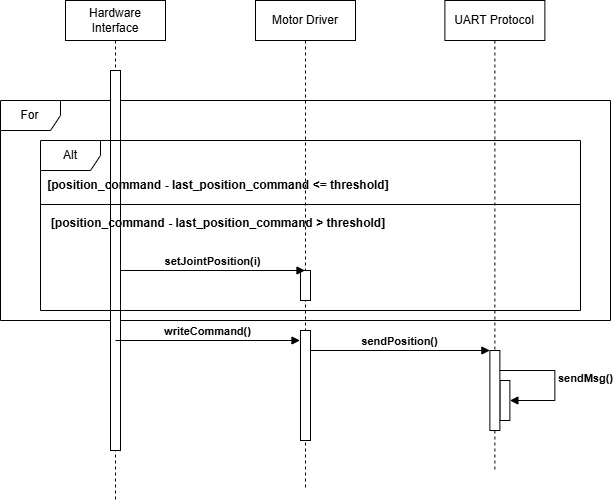
\includegraphics[width=0.8\linewidth]{Images/Implementation/Control/Write_flow.jpg}
    \caption{Luồng điều khiển (Write) của DensoInterface}
    \label{fig:placeholder}
\end{figure}

Đầu tiên, ta sẽ xem xét luồng điều khiển (Write) của DensoInterface. Với mỗi lần tới bước "write" trong chu kì, trước đó "update" đã thực hiên ghi lệnh điều khiển tiếp theo vào "command interface", trong trường hợp này là \lstinline[style=inlinecode]{joint_position_command_[i]}. \lstinline[style=inlinecode]{write} sẽ tiến hành so sánh giữa lệnh điều khiển hiện tại và lệnh điều khiển trước đó có khoảng cách đủ dài (về vị trí) không, tức ta sẽ chỉ cho cánh tay xoay khi sự thay đổi về vị trí (góc xoay) đủ lớn, khi threshold >= 0.001 (rad). Nếu sự thay đổi về vị trí lớn hơn mức ngưỡng 0.001 (rad), hàm \lstinline[style=inlinecode]{setJointPosition()} được gọi với thông tin trục cần xoay và lệnh điều khiển tương ứng với trục đó. Tuy nhiên, trước khi gọi hàm \lstinline[style=inlinecode]{setJointPosition()}, hàm "write" của DensoInterface có thêm cơ chế đặc biệt, gọi là "Trend Learning", với mục tiêu xem xét chuỗi lệnh nhận được có xu hướng tăng hay giảm, và khi phát hiện xu hướng, sẽ cố gắng giữ vững xu hướng đó cho một chuỗi lệnh liên tục tiếp theo. Chức năng này sẽ được bàn luận chi tiết hơn khi trình bày khối MoveIt Servo.

Lưu ý hàm \lstinline[style=inlinecode]{setJointPosition()} chỉ thực hiện việc ghi giá trị điều khiển và lưu giữ giá trị đó cho từng trục vào Motor Driver. Để có thể chính thức sử dụng giá trị lưu giữ, DensoInterface sẽ gọi hàm \lstinline[style=inlinecode]{writeCommand()} từ Motor Driver, Motor Driver sẽ thu thập giá trị điều khiển của 6 trục, đóng gói lại thành một mảng \lstinline[style=inlinecode]{vector<double>}. Sau cùng, hàm \lstinline[style=inlinecode]{sendPosition()} được gọi với giá trị của 6 trục, tạo thành một lệnh điều khiển UART với định dạng phù hợp có thể hiểu được bởi máy RC5, gửi xuống RC5 bằng lệnh \lstinline[style=inlinecode]{sendMsg()}.

% \begin{figure}[H]
%     \centering
%     \includegraphics[width=0.72\linewidth]{Images/Implementation/Control/DensoHand_Write_flow.jpg}
%     \caption{Luồng điều khiển (Write) của DensoHandInterface}
%     \label{fig:denso-hand-write-flow}
% \end{figure}

Đối với DensoHandInterface, cơ chế điều khiển được lược bỏ khối trend learning do nhu cầu điều khiển đơn giản. Hiện tại, Servo Driver sẽ đảm nhận việc chuẩn bị chuỗi JSON hợp lệ để điều khiển, và đoạn chuỗi đó được gửi tới Driver-Hat-A với hàm \lstinline[style=inlinecode]{sendMsgWithCLRF()} của UartProtocol. Trong tương lai, đề tài sẽ chuyển việc chuẩn bị chuỗi điều khiển hợp lệ từ UartProtocol lên khối Motor Driver của DensoInterface, để phần UartProtocol chỉ cung cấp những API cơ bản nhất cho truyền nhận. Điều này sẽ giúp tạo nên sự nhất quán trong cách thiết kế của chương trình.

\subsubsection{Luồng đọc (Read)}

\begin{figure}[H]
    \centering
    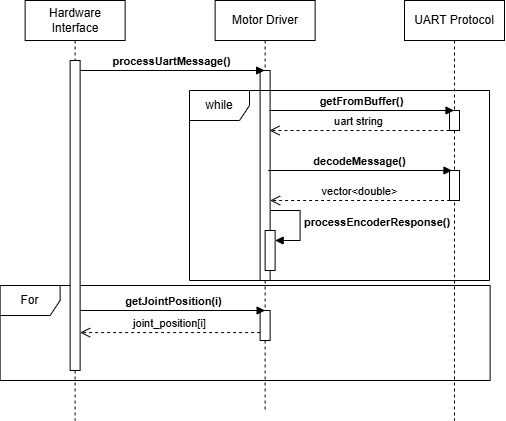
\includegraphics[width=0.8\linewidth]{Images/Implementation/Control/Read_flow.jpg}
    \caption{Luồng đọc (Read) của DensoInterface}
    \label{fig:placeholder}
\end{figure}

Trong luồng đọc của Arctos Interface, dữ liệu thực tế được phản hồi từ cánh tay cần được xử lý và đọc vào các state interfaces. Ở đầu hàm \lstinline[style=inlinecode]{read}, \lstinline[style=inlinecode]{processUartMessage()} của Motor Driver được gọi. Trong \lstinline[style=inlinecode]{processUartMessage}, hàm sẽ lần lượt lấy từng dữ liệu UART nhận được từ buffer của module UART và thực hiện decode (giải mã) nó theo format dữ liệu đã được đề xuất ở phần trước, sử dụng hàm decode được hỗ trợ từ module Uart. Sau khi decode, ta có được giá trị góc xoay của cả 6 trục trong một mảng số thực. Các giá trị góc xoay này sẽ lần lượt được lưu vào \lstinline[style=inlinecode]{JointConfig} của từng trục, sẵn sàng để được truy vấn.

Sau khi đã phân tích hết toàn bộ dữ liệu trong buffer UART, DensoInterface sẽ gọi \lstinline[style=inlinecode]{getJointPosition()} để lấy dữ liệu vị trí đã lưu bởi Motor Driver, cập nhật vào từng state interface tương ứng: \lstinline[style=inlinecode]{joint_position_[i]}.

% \begin{figure}[H]
%     \centering
%     \includegraphics[width=0.72\linewidth]{Images/Implementation/Control/DensoHand_Read_flow.jpg}
%     \caption{Luồng đọc (Read) của DensoHandInterface}
%     \label{fig:denso-hand-read-flow}
% \end{figure}

Chuyển qua luồng đọc của DensoHandInterface, ta cần trước nhất gọi \lstinline[style=inlinecode]{writeQueryCommand()} xuống tay gắp để hỏi trạng thái (vì trạng thái không được liên tục gửi lên như phía cánh tay). Sau khi nhận được phản hồi, hàm \lstinline[style=inlinecode]{processUartMessage()} của ServoDriver thực hiện công việc liên tục lấy chuỗi UART từ buffer đã lưu, và thực hiện decode, bóc tách dữ liệu JSON ngay trên Servo Driver. Giá trị "pos" từ câu trả lời của Driver-Hat-A được tính toán thêm một số bước để chuyển thành giá trị góc phù hợp, đơn vị rad, và gán vào state interface của DensoHandInterface.

\subsection{Ros2 Controllers}

Ros2 controllers là lớp thứ 3 trong kiến trúc Ros2 Control, đảm nhiệm vai trò tạo ra những bộ điều khiển (controller) làm nhiệm vụ cập nhật (update) trong chuỗi chu kì ba bước: read-update-write. Với việc dùng Ros2 Control, người dùng có thể tự mình viết một bộ controller riêng, hoặc tận dụng những controller đã được phát triển sẵn bởi framework. Những controller được phát triển này đã được tổng quát hóa để phù hợp cho nhiều loại robot thông dụng khác nhau, cũng như có khả năng tích hợp tốt với MoveIt2 và Nav2. Chính vì vậy, đề tài ưu tiên sử dụng ba loại controller thông dụng cho dự án cánh tay robot có kèm tay gắp, bao gồm: JointTrajectoryController, GripperActionController và JointStateBoardcaster. Mỗi loại controller được khởi tạo với một tên riêng biệt, nhằm phục vụ mục tiêu điều khiển khác nhau.

Trước nhất, ta cần cấu hình thuộc tính chung cho controller manager trong file ros2\_controller.yaml, cụ thể:

\begin{lstlisting}
controller_manager:
  ros__parameters:
    update_rate: 10 #Hz
    denso_arm_controller:
      type: joint_trajectory_controller/JointTrajectoryController

    denso_hand_controller:
      type: position_controllers/GripperActionController

    joint_state_broadcaster:
      type: joint_state_broadcaster/JointStateBroadcaster
\end{lstlisting}

Phần cấu hình này gồm 2 phần quan trọng: cấu hình update\_rate, là chu kì hoạt động của 1 chu trình read-update-write, và khai báo danh sách các tên controller kèm theo loại của chúng. Chu kì hoạt động hiện tại đang được chọn là 10Hz, nghĩa là mỗi chu kì read-update-write sẽ xảy ra mỗi 100ms. Mặc dù chu kì hoạt động khá thấp so với các dự án khác, tuy nhiên lại là một giá trị phù hợp và đem lại sự ổn định cho hệ thống hiện tại. Lý do của việc cập nhật và điều khiển mỗi 100ms là do:

\begin{itemize}
    \item Máy RC5 xử lý nhận string UART mỗi 10ms.
    \item Khi truyền lệnh điều khiển (write) từ RC5 xuống UART, lệnh sẽ phải được phân tích theo dạng chuỗi một cách thủ công, mất khoảng 20-30ms
    \item Khi xử lý lệnh xong, cánh tay robot cần mất một khoảng thời gian để xoay. Do giới hạn về mặt cơ học cánh tay, cánh tay có thể không thể đạt đến vị trí yêu cầu trong khoảng thời gian ngắn. 
\end{itemize}

Với 100ms, trừ đi thời gian nhận UART và xử lý lệnh điều khiển, cánh tay sẽ có tối thiểu 60ms để xoay tới vị trí được yêu cầu cho tới khi nhận lệnh tiếp theo, là một khoảng thời gian phù hợp, xem xét giới hạn về mặt cơ học hiện tại. Thử nghiệm cho thấy cánh tay sẽ quay tới vị trí yêu cầu trễ khoảng 1-2s cho một lần planning và execute với MoveIt2. Mặt khác, việc tăng tần số lên sẽ chỉ khiến số lượng lệnh gửi xuống tăng lên nhiều hơn, thời gian robot đươc phép xoay sẽ giảm, từ đó làm tăng cao thời gian trễ cho mỗi lần thực hiện chuỗi hành động xoay. 

Tiếp đến, cấu hình của từng controller, và cách nó liên kết với hardware interface sẽ được trình bày.

\subsubsection{denso\_arm\_controller}

"Denso\_arm\_controller" thuộc loại JointTrajectoryController, đóng vai trò chính trong việc vận hành hoạt động của cánh tay robot. Trang \href{https://control.ros.org/humble/doc/ros2_controllers/joint_trajectory_controller/doc/userdoc.html}{JointTrajectoryController} của Ros2-Control cung cấp chi tiết cách để cấu hình và sử dụng loại controller này, cũng như những chức năng mà controller hỗ trợ. Cấu hình cho phần Denso\_arm\_controller hiện tại bao gồm danh sách các trục sẽ điều khiển, state interface, command interface cùng một số thuộc tính đặc biệt:

\begin{lstlisting}
denso_arm_controller:
  ros__parameters:
    joints:
      - X_joint
      - Y_joint
      - Z_joint
      - A_joint
      - B_joint
      - C_joint
    command_interfaces:
      - position
    state_interfaces:
      - position

    state_publish_rate: 25.0
    action_monitor_rate: 10.0

    allow_partial_joints_goal: false
    state_tolerance_check: false  # Disable tolerance checking for simplicity

    allow_nonzero_velocity_at_trajectory_end: true
\end{lstlisting}

Cấu hình hiện tại cho biết Denso\_arm\_controller sẽ có 6 trục, mỗi trục đều có position interface cho command (lệnh điều khiển) và state (trạng thái). Khi chạy controller, trạng thái của controller được cung cấp ở dạng topic với tần số 25hz, và khi thực hiện action, việc theo dõi sự thay đổi trạng thái được thực hiện với tần số 10hz. Tuy nhiên, việc cấu hình ở file yaml là chưa đủ để có thể khởi chạy một luồng ros2-control gồm controller-interface hoàn chỉnh, mà nó cần có sự ràng buộc ở nhiều vị trí khác nhau để đảm bảo liên kết giữa các module được đồng nhất. Cụ thể, cấu hình "6 trục, mỗi trục đều có position interface cho command (lệnh điều khiển) và state (trạng thái)" cần tương đồng trong:

\begin{enumerate}
    \item \textbf{File Urdf}: Dưới tag <ros2\_control>, ngoài thông tin về plugin "hardware interface" sẽ sử dụng, cần liệt kê rõ các joint với tên trùng với tên joint đã cấu hình trong file yaml, đi kèm với command interface và position interface. Ví dụ của trục "X\_joint" dưới tag <ros2\_control> và các trục khác phải có cấu trúc:
    \begin{lstlisting}[language=xml]
    <joint name="X_joint">
        <command_interface name="position">
          <param name="min">-2.967060</param>
          <param name="max">2.967060</param>
        </command_interface>
        <state_interface name="position">
          <param name="initial_value">${initial_positions['X_joint']}</param>
        </state_interface>
    </joint>
    \end{lstlisting}
    \item \textbf{File hiện thực DensoInterface}: Ở bước export state/command interface, loại và số lượng interface cho từng trục cần được export đủ và chính xác, ví dụ:
    \begin{lstlisting}[language=C]
state_interfaces.emplace_back(
            info_.joints[i].name, hardware_interface::HW_IF_POSITION, &joint_position_[i]);
...
command_interfaces.emplace_back(
            info_.joints[i].name, hardware_interface::HW_IF_POSITION, &joint_position_command_[i]);
    \end{lstlisting}
    Hai câu lệnh trên đảm bảo joint với tên được ghi trong URDF dưới tag <ros2\_control> (ví dụ X\_joint) sẽ được cung cấp hai command interface và state interface loại Position bởi DensoInterface.
\end{enumerate}

Nếu có sự không đồng nhất giữa cấu hình file yaml, urdf hoặc cách hardware interface export, controller tương ứng sẽ không khởi chạy.

Khi cấu hình hoàn chỉnh và khởi chạy được denso\_arm\_controller, controller này sẽ cung cấp hai cách thức để điều khiển: 

\begin{itemize}
    \item Thông qua Action: denso\_arm\_controller/follow\_joint\_trajectory
    \item Thông qua Ros topic: denso\_arm\_controller/joint\_trajectory
\end{itemize}

Hai cách thức giao tiếp này sẽ được tận dụng bởi MoveIt2 trong chức năng planning và moveit servo. Chi tiết này sẽ được trình bày cụ thể hơn ở phần sau.

\subsubsection{denso\_hand\_controller}

"Denso\_hand\_controller" thuộc loại \textbf{GripperActionController}, là một loại controller đơn giản hơn với mục tiêu là điều khiển loại tay gắp hai đầu song song (parallel gripper). Tượng tự, cách cấu hình trong file ros2\_controlles.yaml có thể tham khảo ở trang \href{https://control.ros.org/humble/doc/ros2_controllers/gripper_controllers/doc/userdoc.html}{Gripper Action Controller}. Cấu hình hiện tại cho phần tay gắp là:

\begin{lstlisting}
denso_hand_controller:
  ros__parameters:
    joint: gripper_gear_right_joint

    goal_tolerance: 0.1               # rad
    stall_velocity_threshold: 0.001   # rad/s
    stall_timeout: 2.0                # seconds
    action_monitor_rate: 10.0         # Hz
\end{lstlisting}

So với JointTrajectoryController, GripperActionController chỉ điều khiển duy nhất một trục, và các tham số cấu hình cũng tương đối đơn giản. GripperActionController có yêu cầu cố định về interface, phải có hai state interface: velocity, position và một command interface: position. Về mặt điều khiển, chỉ cần cấu hình phần joint của tay gắp bên trái, phần joint còn lại sẽ bắt chước - mimic theo trong minh họa Rviz cũng như Gazebo. Các thông số liên quan tới tolerance, stall được chỉnh tương đối để tạo sự thoải mái trong điều khiển.

Tương tự, để có thể khởi chạy denso\_hand\_controller, ta cần đảm bảo những cấu hình ở các file liên quan được đồng nhất, cụ thể:

\begin{enumerate}
    \item Trong tag <ros2\_control> cho controller tay gắp, chỉ cần để một joint duy nhất, kèm theo một position interface và hai state interface. Tuy vậy, chỉ có position state interface sẽ được sử dụng trong dự án.
    \begin{lstlisting}[language=xml]
    <joint name="gripper_gear_right_joint">
        <command_interface name="position">
          <param name="min">0.087266</param>
          <param name="max">1.48353</param>
        </command_interface>
        <state_interface name="position">
          <param name="initial_value">${initial_positions['gripper_gear_right_joint']}</param>
        </state_interface>
        <state_interface name="velocity" />
    </joint>
    \end{lstlisting}
    \item Trong DensoHandInterface, các interfaces tương ứng cũng cần được export dầy đủ:
    \begin{lstlisting}
state_interfaces.emplace_back(
            info_.joints[i].name, hardware_interface::HW_IF_POSITION, &servo_position_[i]);
    ...
state_interfaces.emplace_back(
            info_.joints[i].name, hardware_interface::HW_IF_VELOCITY, &servo_velocity_[i]);
    ...
command_interfaces.emplace_back(
            info_.joints[i].name, hardware_interface::HW_IF_POSITION, &servo_position_command_[i]);
    \end{lstlisting}
\end{enumerate}

Denso\_hand\_controller cung cấp một phương thức giao tiếp duy nhất là thông qua \href{https://docs.ros.org/en/melodic/api/control_msgs/html/action/GripperCommand.html}{GripperCommand Action}, cụ thể: /denso\_arm\_controller/GripperCommand. Action server này được sử dụng bởi MoveIt2 cho planning, và cũng là cách điều khiển mà ứng dụng VR sử dụng để có thể nhanh chóng điều khiển tay gắp.

\subsubsection{joint\_state\_boardcaster}

Joint\_state\_boardcaster - như tên gọi - là một controller không phải để điều khiển thiết bị, mà là để thông báo (boardcast) dữ liệu. Đây cũng là một controller quan trọng, có nhiệm vụ thu thập toàn bộ state interface liên quan tới Joint và publish nó lên topic \textbf{/joint\_states}, cung cấp dữ liệu thực tế của phần cứng cho các ứng dụng quan tâm. Đối với controller này, đề tài để mọi thông số ở dạng mặc định và không tùy chỉnh gì thêm.

\subsection{Moveit2}

MoveIt2 là lớp thứ 4 trong kiến trúc đề xuất này, đóng vai trò là một giải pháp giúp điều khiển robot một cách hiệu quả với sự tích hợp chặt chẽ với Ros2-Control. Moveit2 sẽ tự động kết nối với Ros2-Control để điều khiển các Controller thực hiện chức năng "update". \href{https://moveit.picknik.ai/humble/doc/examples/setup_assistant/setup_assistant_tutorial.html}{MoveIt Setup Assistant} là một bộ tool được đề tài tận dụng để có thể sinh ra những file cấu hình cần thiết cho việc sử dụng MoveIt2, cũng như tạo sự liên kết giữa MoveIt2 và các Ros2-Controller đã chuẩn bị. Bộ tool hỗ trợ sinh ra thư mục "moveit\_config", gồm một số file chính như sau:

\begin{Verbatim}
moveit_config
└── config
    ├── arctos.srdf
    ├── initial_positions.yaml
    ├── joint_limits.yaml
    ├── chomp_planning.yaml
    ├── kinematics.yaml
    ├── moveit_controllers.yaml
    ├── moveit.rviz
    ├── pilz_cartesian_limits.yaml
    └── ros2_controllers.yaml
\end{Verbatim}

\begin{itemize}
    \item \textbf{arctos.srdf}: khác với file URDF có vai trò đặc tả về cấu trúc của robot, file SRDF (Semantic Robot Description Format) dùng để định nghĩa những thông tin ngữ nghĩa (semantic) cho robot. Ở đây có thể định nghĩa một nhóm các trục để điều khiển - planning trong \lstinline[style=inlinecode]{<group>}, định nghĩa trạng thái nhóm các trục và vị trí các trục ở trạng thái đó trong \lstinline[style=inlinecode]{<group_state>}. \lstinline[style=inlinecode]{<disable_collisions>} hữu dụng trong quá trình mô phỏng cánh tay robot, với khả năng tắt tính toán va chạm giữa những bộ phận của robot do nhiều lý do khác nhau, qua đó tăng tốc thời gian tính toán va chạm, cho phép MoveIt có thể lập ra những kế hoạch di chuyển (planning) chính xác, hiệu quả cho cánh tay robot.
    \item \textbf{chomp\_planning.yaml}: File cấu hình thuật toán tính toán lập quỹ đạo chuyển động Covariant Hamiltonian Optimization for Motion Planning (CHOMP). 
    \item \textbf{initial\_positions.yaml}: Vị trí ban đầu của từng trục cánh tay
    \item \textbf{joint\_limits.yaml}: Một file cấu hình khác cho phép ghi đè những thuộc tính trên file URDF của cánh tay, cụ thể là cấu hình về vận tốc và gia tốc tối đa. Việc cấu hình tốc độ/gia tốc tối đa có ảnh hưởng tương đối với MoveIt trong quá trình lập kế hoạch di chuyển của các trục, bởi MoveIt sẽ điều chỉnh vị trí và vận tốc linh hoạt, có tăng tốc ở khoảng bắt đầu và giảm tốc ở khoảng kết thúc, vận tốc trong quá trình di chuyển giữa sẽ gần đạt tối đa. Chính vì vậy, vận tốc tối đa càng cao, thời gian xoay cánh tay và số bước thực hiện hành động xoay càng ngắn. Ngược lại, vận tốc tối đa càng thấp, số bước di chuyển càng nhiều và cánh tay sẽ xoay chậm hơn.
    \item \textbf{kinematics.yaml}: File lựa chọn thuật toán động học sử dụng, thời gian tìm kiếm lời giải và timeout khi lời giải không thể tìm thấy.
    \item \textbf{ros2\_controllers.yaml}: Bộ tool khi đọc file urdf có chứa tag <ros2\_control>, sẽ cho phép người dùng cấu hình các controller ngay trong giao diện tool. Tại đây ta có thể định nghĩa tên controller và gán loại controller tương ứng, gán các joint sẽ sử dụng cho controller, và xác định các interface được sử dụng. 
    \item \textbf{moveit\_controllers.yaml} Sau khi cấu hình các controller, tool sẽ cho phép cấu hình phần "moveit controller \textbf{manager}". "Moveit\_simple\_controller\_manager" được sử dụng để quản lý các controller từ phía Ros2-Control, khai báo loại controller và các tên trục mà MoveIt sẽ điều khiển. Điều này giúp MoveIt2 biết rằng nó nên giao tiếp với Action Server của FollowJointTrajectory cho việc điều khiển cánh tay thông qua controller denso\_arm\_controller, và Action Server GripperCommand để điều khiển tay gắp thông qua denso\_hand\_controller.
\end{itemize}

Khi Cấu hình và khởi chạy thành công, MoveIt2 sẽ cho phép người dùng sử dụng tính năng "Planning" để tính toán quỹ đạo chuyển động tới một vị trí cụ thể (dựa vào tọa độ, hoặc giá trị các trục ở vị trí đích). Cơ chế planning này cũng sẽ hỗ trợ trong việc tính toán quỹ đạo chuyển động né vật cản được tạo trong môi trường Rviz, tùy theo yêu cầu của bài toán cần phát triển. Việc tính toán quỹ đạo chuyển động có thể được tùy chỉnh để dùng nhiều loại thuật toán khác nhau, và hiện tại đề tài đang dùng mặc định thuật toán CHOMP cho tính toán. Khi thấy planning đã ổn định, tính năng "Execute" yêu cầu MoveIt2 điều khiển các controller để xoay cánh tay robot theo quỹ đạo đã tính toán. Nhờ có sự trợ giúp của MoveIt2, các quỹ đạo đươc tính ra thường đã bao gồm tinh chỉnh, có sự tăng tốc ở giai đoạn đầu quỹ đạo và giảm tốc ở giai đoạn cuối, để giúp cho chuyển động trên quỹ đạo được mượt mà khi các lệnh điều khiển được gửi xuống khối controller.  

Ngoài khối planning, MoveIt2 cũng hỗ trợ package \href{https://moveit.picknik.ai/main/doc/examples/realtime_servo/realtime_servo_tutorial.html}{"MoveIt Servo"}, hay còn gọi là "Real-time Servo", cho nhu cầu điều khiển một hoặc nhiều trục xoay liên tục một góc nhỏ, hoặc điều khiển cánh tay di chuyển theo tọa độ X,Y,Z. Chi tiết tính năng này sẽ được trình bày ở khối sau.

\subsection{Khối ứng dụng}

Khối ứng dụng bao gồm các khối các module nhỏ riêng biệt, được phát triển dựa trên sự hỗ trợ của MoveIt2 cho để điều khiển cánh tay robot thực tế. Ở lớp này, nhiều loại ứng dụng có thể được phát triển, tuy nhiên trong giới hạn đề tài hiện tại sẽ chỉ xây dựng lớp ứng dụng để cung cấp phương thức điều khiển cho thành phần bên ngoài muốn giao tiếp với hệ thống. Hiện tại, khối ứng dụng cho phép thiết bị bên ngoài (Kính VR) giao tiếp với Ros2 bên trong thông qua Denso Moveit Servo (Service Provider) và Denso Remote Control (Action Server).

\subsubsection{Denso MoveIt Servo}

Denso MoveIt Servo là một Ros2 Service Provider, đóng vai trò như một Wrapper trên Ros2-Moveit-Servo để cung cấp khả năng điều khiển robot xoay từng trục hoặc theo tọa độ. Moveit-Servo cho phép người dùng thực hiện cấu hình cách hoạt động của module này qua file yaml, trong đó một số bộ cấu hình quan trọng có thể kể đến như:

\begin{lstlisting}
## Properties of outgoing commands
publish_period: 0.3  # 1/Nominal publish rate [seconds] 

# What type of topic does your robot driver expect?
command_out_type: trajectory_msgs/JointTrajectory

# What to publish?
publish_joint_positions: true
publish_joint_velocities: false
publish_joint_accelerations: false

## Plugins for smoothing outgoing commands
smoothing_filter_plugin_name: "online_signal_smoothing::ButterworthFilterPlugin"
\end{lstlisting}

Publish period là thời gian giữa các lệnh gửi điều khiển từ MoveIt-Servo. Với MoveIt-Servo, sẽ có hai luồng điều khiển: từ người dùng gửi lệnh tới MoveIt-Servo, và từ MoveIt-Servo sẽ tiến hành tính toán, đưa ra lệnh phù hợp để gửi thẳng tới Ros2-controller được cấu hình, thông qua topic thuộc loại "command\_out\_type". Với Publish period là 0.3, có nghĩa là cứ 300ms, MoveIt-Servo sẽ gửi một chuỗi quỹ đạo (JointTrajectory) tới Ros2-controller loại FollowJointTrajectory để yêu cầu xoay cánh tay, thay vì thông qua Action Server mà MoveIt2 sử dụng cho module planning thông thường. Điều này giúp MoveIt-servo có thể điều khiển thiết bị nhanh mà không bị ảnh hưởng bởi thời gian xử lý tương đối chậm của Action Server. Thêm nữa, ButterworthFilterPlugin được sử dụng để "lọc" dữ liệu điều khiển truyền ra, giúp các lệnh điều khiển ổn định và đảm bảo robot có thể xoay đều, mượt mà. 

\begin{lstlisting}
## Stopping behaviour
# Stop servoing if X seconds elapse without a new command
incoming_command_timeout:  0.3  
\end{lstlisting}

Một trong những vấn đề khi hiện thực việc điều khiển robot xoay liên tục, đó là xác định khi nào nên dừng việc xoay. MoveIt-Servo giải quyết điều này dễ dàng qua việc cho phép người dùng điều chỉnh thông số timeout, trong trường hợp này là 300ms; nghĩa là người dùng có thể spam liên tục lệnh điều khiển gửi tới MoveIt-Servo, tuy nhiên nếu ngưng gửi lệnh và MoveIt-Servo nhận thấy đã quá 300ms kể từ khi nhận lệnh cuối cùng, MoveIt-Servo cũng sẽ ngưng gửi lệnh JointTrajectory xuống controller, từ đó ngưng xoay robot thực tế. 

Tuy nhiên, cơ chế này lại mang tính ràng buộc về thời gian thực (Real-time) để có thể hoạt động chính xác. Cụ thể, cách MoveIt-Servo xác định timeout là lấy thời điểm trong Header TimeStamp có trong mỗi lệnh gửi tới MoveIt-Servo, trừ với thời gian thực tế (Ros wall-timer), điều này yêu cầu lệnh gửi tới phải có TimeStamp hợp lệ để MoveIt-Servo có thể tính toán và cho dừng hoạt động điều khiển sau khoảng thời gian timeout. 

\begin{lstlisting}
## Topic names
cartesian_command_in_topic: ~/delta_twist_cmds  
joint_command_in_topic: ~/delta_joint_cmds
joint_topic: /joint_states
status_topic: ~/status 
command_out_topic: /denso_arm_controller/joint_trajectory 
\end{lstlisting}

Phần cấu hình này giúp định nghĩa tên của các topic gửi tới MoveIt-Servo (in\_topic) và topic được gửi ra từ MoveIt-Servo tới Ros2-Controller (out\_topic). Như đã trình bày ở trên, MoveIt-Servo cho phép di chuyển cánh tay theo trục (joint\_command) hoặc theo tọa độ cartesian (cartesian\_command), tuy nhiên đề tài chủ yếu sử dụng joint\_command. Việc di chuyển theo tọa độ đề các còn một số điểm bất ổn định và cần nhiều kiểm tra kĩ hơn trước khi sử dụng chính thức. 

joint\_topic được cung cấp để giúp MoveIt-Servo tính toán quỹ đạo từ vị trí hiện tại của cánh tay. Chính vì vậy, trong trường hợp cánh tay thực tế quay trễ hơn so với lệnh điều khiển, cơ chế này sẽ khiến cánh tay bị "giật lùi". Giả sử, trục X được MoveIt-Servo tính toán, và gửi quỹ đạo quay lần lượt là [3, 5, 10, 15], mong đợi rằng cánh tay sẽ xoay tới vị trí 15 độ sau 300ms. Tuy nhiên, 300ms sau, cánh tay thực tế chỉ mới quay tới 7 độ (trạng thái của joint\_states), nên MoveIt-Servo tính lại quỹ đạo: [7, 10, 15, 18]. Tuy nhiên, lệnh 10, 15 đã được gửi tới Ros2-Control, và Ros2-Control đã truyền chúng xuống RC5 để thực thi, dẫn tới RC5 sẽ nhận chuỗi lệnh là: [3, 5, 10, 15, \textbf{7, 10, 15}, 18]. Trục X sẽ bị điều khiển xoay tới 15 độ rồi giật ngược về 7 độ, xoay tiếp lên 10, 15 trở lại.

Để tạm thời giải quyết vấn đề từ MoveIt-Servo có mong đợi không chính xác về thời gian xoay của cánh tay, cũng như độ trễ do tính chất cơ khí của cánh tay robot, đề tài hiện thực cơ chế Trend Learning ở lớp DensoInterface như đã trình bày ở phần trước, nhằm mục tiêu phát hiện chuỗi lệnh có xu hướng tăng/giảm, nên khi nhận lệnh giật lùi trong một khung thời gian nhỏ từ MoveIt-Servo tới denso\_arm\_controller, xuống DensoInterface, các lệnh giật lùi sẽ bị loại bỏ và thay bằng một giá trị hợp lệ trước đó + padding nhỏ. Điều này giúp giải quyết:

\begin{itemize}
    \item Loại bỏ tình huống giật lùi do cánh tay xoay chậm hơn so với mong đợi từ MoveIt-Servo
    \item Các lệnh giật lùi bị thay thế bằng giá trị hợp lệ cuối + padding thay vì ngưng gửi giúp cho RC5 luôn luôn có lệnh điều khiển ở mỗi chu kì của Ros2-control (100ms). Điều này giúp buffer RC5 sẽ luôn có lệnh và đảm bảo trục được xoay liên tục, tránh trường hợp xuất hiện khoảng trống lệnh, khiến trục xoay bị giật (giảm tốc và dừng vì đạt tới vị trí yêu cầu và không có lệnh mới (khoảng trống), sau đó lệnh hợp lệ mới được đưa vào, trục phải khởi động và tăng tốc để xoay)
\end{itemize}

Ngoài ra, MoveIt-Servo cũng đảm bảo rằng việc xoay từng trục được giới hạn bởi các limit được cấu hình từ file Urdf, khi gần chạm tới ngưỡng xoay của trục thì lệnh yêu cầu xoay sẽ bị chặn lại, không gửi tới Ros2-Controller, đảm bảo cho cánh tay hoạt động trong ngưỡng an toàn. 

Denso MoveIt Servo, như đã trình bày, sẽ có vai trò khởi tạo Node MoveIt-Servo với những cấu hình từ file yaml đã mô tả, từ đó cung cấp cho người sử dụng hai topic để điều khiển:

\begin{itemize}
    \item denso\_moveit\_servo\_node/delta\_twist\_cmds [geometry\_msgs::msg::TwistStamped]
    \item denso\_moveit\_servo\_node/delta\_joint\_cmds [control\_msgs::msg::JointJog] (*)
\end{itemize}

Kèm theo đó, hai dịch vụ (service) được cung cấp để cho phép sử dụng/ tắt MoveIt-Servo:

\begin{itemize}
    \item denso\_moveit\_servo\_node/start\_servo [std\_srvs::srv::Trigger]
    \item denso\_moveit\_servo\_node/stop\_servo [std\_srvs::srv::Trigger]
\end{itemize}

Chỉ khi dịch vụ ~/start\_servo được gọi, thì các lệnh gửi đến 2 topic delta\_twist\_cmds / delta\_joint\_cmds mới được xử lý bởi MoveIt-Servo. Ngược lại, nếu ~/stop\_servo được gọi, thì MoveIt-Servo sẽ không hoạt động, cho tới khi ~/start\_servo được trigger.

\subsubsection{Denso Remote Control}

Denso Remote Control được thiết kế ở dạng một Action Server, với mục tiêu cung cấp cho thiết bị bên ngoài phương thức để gửi lệnh điều khiển cánh tay tới một vị trí cụ thể (thông qua giá trị của 6 trục hoặc tọa độ XYZ) xuống MoveIt để planning và thực thi. Lý do lựa chọn Action Server thay vì Service Provider là vì thao tác Planning, đặc biệt là Execute của MoveIt có thời gian thực hiện dài, nên dùng Action Server sẽ giúp cho thiết bị bên ngoài có thể gửi mục tiêu (Goal) và theo dõi trạng thái thực thi cho tới khi hoàn thành. 

Denso Remote Control sử dụng một định dạng Action riêng, gọi là \textbf{MoveToPose}, bao gồm ba message:

\begin{lstlisting}[language={}]
# Request
geometry_msgs/Pose pose
float64[] joints
bool use_pose
---
#Result
bool completed
---
#Feedback
string step
\end{lstlisting}

Trong đó, Request sẽ chấp nhận message dạng geometry\_msgs/Pose (mô tả tọa độ XYZ và góc xoay của phần đầu cánh tay - end effector) hoặc giá trị góc (độ) của sáu trục cánh tay robot. Biến bool use\_pose dùng để quyết định message pose sẽ được sử dụng (true) hay chuỗi sáu góc của cánh tay robot sẽ được sử dụng (false). Result là \lstinline[style=inlinecode]{bool completed}, cho biết Action server đã hoàn thành công việc chưa, và \lstinline[style=inlinecode]{string step} cập nhật trạng thái của từng bước hoạt động của action server, trong quá trình nhận lệnh, planning và execute từ phía MoveIt.

Luồng hoạt động và phản hồi của Denso Remote Control khi có request từ Action client sẽ theo như hình:

\begin{figure}[H]
    \centering
    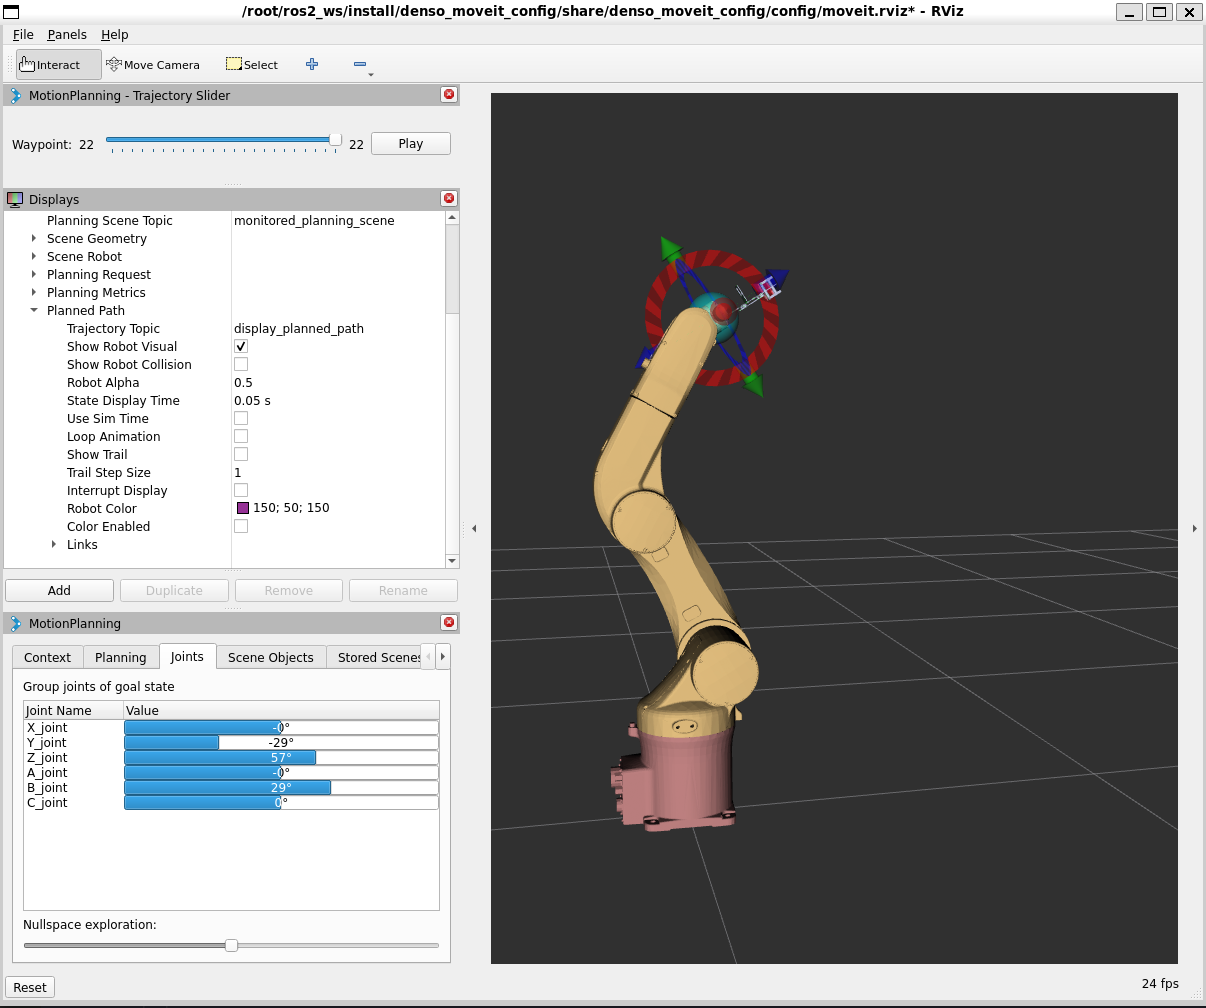
\includegraphics[width=0.75\linewidth]{Images/Implementation/remote_control_1.png}
    \caption{Luồng hoạt động của Denso Remote Control Action Server}
    \label{fig:denso-remote-control-flow}
\end{figure}

\begin{enumerate}
    \item Khi nhận một Goal request, kiểm tra \lstinline[style=inlinecode]{use\_pose} và quyết định chọn message Pose hay chuỗi góc trục. Nếu request đưa tới là hợp lệ, tiến tới bước planning.
    \item Thực hiện ghi trạng thái đích (sử dụng \lstinline[style=inlinecode]{setPoseTarget()} nếu dùng pose, hoặc \lstinline[style=inlinecode]{setJointValueTarget()} nếu dùng chuỗi góc trục), sau đó tiến hành planning thông qua Moveit. \lstinline[style=inlinecode]{step} hiển thị "planning". Nếu planning thất bại, \lstinline[style=inlinecode]{completed = true} và \lstinline[style=inlinecode]{step = planning_failed:} kèm theo lý do cụ thể.
    \item Sau khi planning thành công, bước execute sẽ khởi chạy sử dụng hàm \lstinline[style=inlinecode]{execute()} của MoveIt, \lstinline[style=inlinecode]{step = executing} và thiết bị sẽ được điều khiển trong suốt thời gian executing. Nếu có lỗi trong quá trình execute, \lstinline[style=inlinecode]{step = execute_failed:} kèm lý do, và \lstinline[style=inlinecode]{completed = true}. Nếu việc execute thành công, \lstinline[style=inlinecode]{step = completed} và \lstinline[style=inlinecode]{completed=true}
\end{enumerate}

Khi khởi chạy, Action client có thể gửi MoveToPose goal request tới Denso Remote Control để thực hiện việc xoay cánh tay robot tới vị trí yêu cầu.

\paragraph{Đánh giá nhanh thiết kế điều khiển}

Thiết kế hiện tại cho thấy sự cân bằng giữa độ ổn định và khả năng mở rộng: các lớp Driver, Hardware Interface, Controller và lớp ứng dụng đã được tách rõ để dễ kiểm thử và bảo trì. Cơ chế CRC theo độ dài payload ở phía RC5 cùng Ring Buffer giúp tăng khả năng chịu lỗi khi truyền UART. Tuy vậy, một số giới hạn vẫn còn tồn tại, điển hình là độ trễ cơ khí khiến MoveIt Servo đôi khi tạo chuỗi lệnh có xu hướng giật lùi; giải pháp Trend Learning ở DensoInterface hiện đang xử lý tốt ở mức ứng dụng, nhưng vẫn cần thêm các thử nghiệm định lượng dài hạn để đánh giá độ bền vững theo nhiều kịch bản tải khác nhau.

\subsection{Mô phỏng với Gazebo}

Trong quá trình phát triển, để giảm bớt sự phụ thuộc vào thiết bị thực tế và tăng tốc thời gian phát triển các module lớp ứng dụng trở lên, Gazebo Ignition được xây dựng để làm hệ thống mô phỏng điều khiển thay thế phần Hardware Interface trở xuống. Việc tận dụng Gazebo trong quá trình phát triển ứng dụng giúp nhà phát triển có thể nhanh chóng kiểm tra cách hoạt động của robot trong chuỗi điều khiển của mình, và thực hiện sửa đổi cho phù hợp, giảm gánh nặng và khả năng lỗi lên thiết bị thực tế. 

Để có thể tích hợp Gazebo vào dự án, ta sẽ cần thực hiện một số thay đổi sau:

\begin{enumerate}
    \item \textbf{Tắt trọng lực, bật động học}: Với mỗi một Link trong file UART, tag gazebo cần được liên kết để tắt tác dụng của trọng lực lên cánh tay. Bật động học đảm bảo cánh tay robot chỉ có thể được điều khiển bởi người dùng, chứ không chịu ảnh hưởng bởi va chạm với vật thể nào khác trong mô phỏng. Điều này giúp cho robot có thể giữ vị trí cố định và điều khiển được.

    \begin{lstlisting}[language=xml]
     <link name="${name}">
     ...
     </link>
    <gazebo reference="${name}">
      <kinematic>true</kinematic>
      <gravity>false</gravity>
    </gazebo>
    \end{lstlisting}
    
    \item \textbf{Thêm thuộc tính friction (ma sát), damping (giảm chấn) vào cho các trục trong file URDF}: Nếu thiếu hai thông số friction và damping, các trục gần như sẽ bị overshoot khi xoay do quán tính, khiến nó xoay xa hơn so với vị trí yêu cầu. Bộ số friction, damping hợp lý sẽ giữ cho cánh tay có được độ ổn định, có thể giữ vị trí góc được điều khiển và xoay với tốc độ gần tương đồng với thiết bị thật. 

        \begin{lstlisting}[language=xml]
    <joint name="${name}" type="${type}">
      ...
      <dynamics damping="${damping}" friction="${friction}"/>
    </joint>
    \end{lstlisting}
    \item \textbf{Tích hợp GazeboSimRos2ControlPlugin vào file URDF}: Gazebo cung cấp khả năng tích hợp dễ dàng với Ros2-Control, người dùng chỉ cần thêm Gazebo như một plugin như sau:

        \begin{lstlisting}[language=xml]
    <gazebo>
      <plugin filename="gz_ros2_control-system" name="gz_ros2_control::GazeboSimROS2ControlPlugin">
        <robot_param>robot_description</robot_param>
        <robot_param_node>robot_state_publisher</robot_param_node>
        <parameters>$(find denso_moveit_config)/config/ros2_controllers.yaml</parameters>
        <controller_manager_name>controller_manager</controller_manager_name>
      </plugin>
    </gazebo>
    \end{lstlisting}

    \item \textbf{Tạo file hook thay đường dẫn mặc định của Gazebo sang Ros2}: Do Gazebo là một phần mềm riêng biệt so với ROS2, nên khi khởi chạy, Gazebo sẽ không biết đường dẫn trỏ tới các tài nguyên như file mô hình 3D (STL) của cánh tay robot. Việc tạo file hooks ở ngay trong robot description sẽ giúp giải quyết vấn đề này.
    
    \item \textbf{Thay thế Hardware Interface với Gazebo}: Gazebo đóng vai trò là một bộ mô phỏng thiết bị vật lý, do đó nó cần đóng vai trò là một Hardware Interface để cung cấp trạng thái, cũng như thực hiện yêu cầu điều khiển. Khi cần sử dụng Gazebo, ta bật \lstinline[style=inlinecode]{sim=True}, và GazeboSimSystem sẽ thay thế HardwareInterface thực tế.

    \begin{lstlisting}[language=xml]
    <hardware>
        <!-- By default, set up controllers for gazebo. This won't work on real hardware -->
        <xacro:if value="${sim}">
          <plugin>gz_ros2_control/GazeboSimSystem</plugin>
        </xacro:if>
        <xacro:unless value="${sim}">
          <plugin>denso_interface/DensoInterface</plugin>
          <param name="device">/dev/ttyUSB0</param>
          <param name="baud_rate">115200</param>
          <param name="timeout">1000</param>
        </xacro:unless>
    </hardware>
    \end{lstlisting}

    \item Sau cùng, ở file launch của dự án, lần lượt khởi chạy Gazebo, sinh mô hình robot bằng cách dọc robot description, Gazebo sẽ xuất hiện và đóng vai trò là bộ mô phỏng cánh tay robot, có thể điều khiển được thông qua MoveIt và Ros2-Control.

\end{enumerate}

\subsection{Lấy dữ liệu camera với V4L2 Camera Node}

Để có thể điều khiển cánh tay robot hiệu quả trong môi trường ảo, việc theo dõi các hình ảnh camera từ hệ thống xung quanh thiết bị thực tế là cần thiết để theo dõi và tăng nhận thức môi trường cho người sử dụng. Chính vì vậy, đề tài chủ trương sử dụng hai camera: camera 1 ở đầu tay gắp và camera 2 bao quát môi trường và cánh tay. Cả hai camera đều là Usb Camera của Ugreen, kết nối trực tiếp tới máy PC Controller.

Để đọc được dữ liệu ảnh từ camera vào Ros2, đề tài sử dụng package \href{https://github.com/tier4/ros2_v4l2_camera}{ros2\_v4l2\_camera} đóng vai trò như ros node truyền dữ liệu camera theo những thông số cấu hình linh động ra các topic thông dụng về dữ liệu ảnh. Ảnh được truyền qua topic với kích thước [640 x 480], định dạng màu rgb8.

Thêm nữa, package \href{https://github.com/ros-perception/image_transport_plugins}{image\_transport\_plugins} được sử dụng để cung cấp khả năng nén ảnh, giúp người dùng có thể truyền dữ liệu ảnh đi với lượng data ít hơn, giảm bớt tải cho đường truyền. Chỉ cần cài đặt image\_transport\_plugins, ros2\_v4l2\_camera sẽ phát hiện plugin này và tự động tạo thêm topic \lstinline[style=inlinecode]{/image_raw/compressed} để truyền dữ liệu đã được nén bởi plugin.

Lệnh cài đặt ros2\_v4l2\_camera và image\_transport\_plugins như sau:

\begin{lstlisting}[style=bashstyle]
    sudo apt install ros-humble-v4l2-camera ros-humble-rqt-image-view ros-humble-image-transport-plugins -y
\end{lstlisting}

Trong đó \lstinline[style=inlinecode]{rqt-image-view} là một package dùng để kiểm tra nhanh chóng dữ liệu hình ảnh được truyền qua topic Camera trong môi trường Ros2.
 
Khi cài đặt và khởi chạy thành công, dữ liệu ảnh từ hai camera sẽ được truyền qua các topic sau đây, cho cả ảnh gốc (image\_raw) và ảnh đã nén (compressed)

\begin{lstlisting}[language={}]
    /camera_1/image_raw
    /camera_1/image_raw/compressed
    /camera_2/image_raw
    /camera_2/image_raw/compressed
\end{lstlisting}
 
\subsection{Sử dụng RosBridge server}

Ros2 cho phép giao tiếp dễ dàng thông qua mạng LAN cho các thiết bị cùng chạy Ros, tuy nhiên đối với kính VR chạy ứng dụng Unity, việc cài đặt và chạy Ros2 là không khả thi. \href{https://github.com/siemens/ros-sharp}{Ros-Sharp} cung cấp giải pháp giao tiếp giữa ứng dụng .Net (C\#, Unity) và Ros2 thông qua Web socket một cách hiệu quả và nhanh chóng.

\begin{figure}[H]
    \centering
    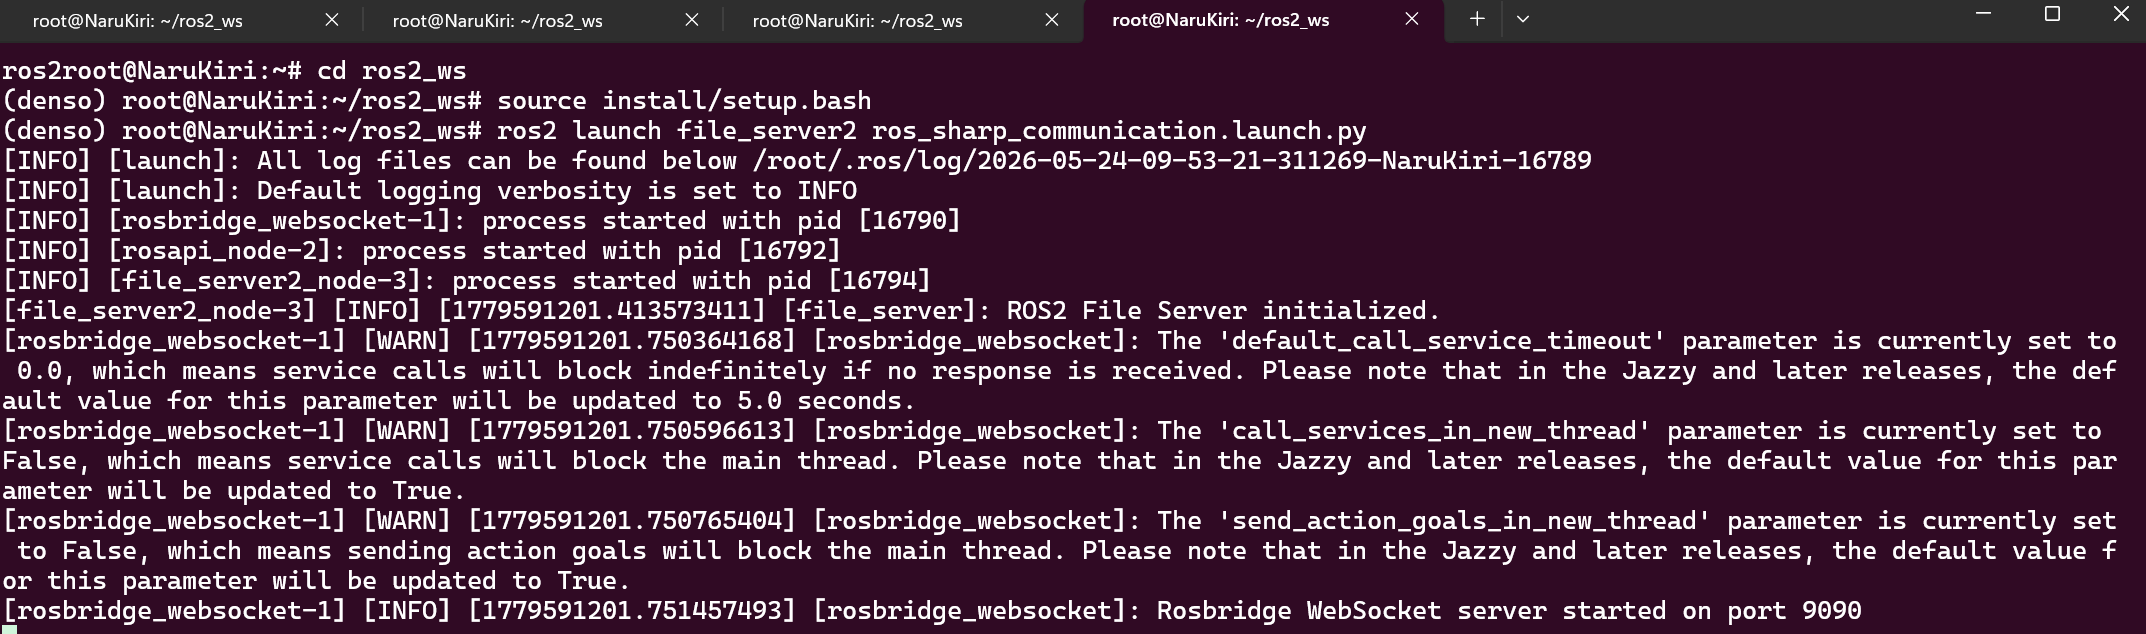
\includegraphics[width=0.8\linewidth]{Images/Implementation/rosbridge_server.png}
    \caption{RosBridge Server làm cầu nối giữa ROS2 và ứng dụng Unity}
    \label{fig:rosbridge-server}
\end{figure}

Để tạo kết nối cho giao tiếp Ros, người dùng cần cài đặt các package hỗ trợ ở cả phía Ros2 và cả Unity. Về phía Ros2, ta sẽ cài đặt RosBridge Server để cho phép ứng dụng Unity có thể kết nối tới. 

\begin{lstlisting}[style=bashstyle]
# Install rosbridge_suite
sudo apt-get install ros-humble-rosbridge-server
\end{lstlisting}

Sau khi cài xong, package \href{https://github.com/siemens/ros-sharp/tree/master/ROS%20Packages/ROS2/file_server2}{file\_server2} từ Repo được sử dụng để khởi chạy RosBridge server cùng một số tham số tùy chỉnh như port, kích thước gói tin, timeout cho service...

Với việc cài đặt RosBridge server, gần như mọi topic, service và action có thể được truy cập bởi ứng dụng .Net sử dụng Ros-sharp. Với đồ án hiện tại, RosBridge Server sẽ cho phép ứng dụng VR truy cập các topic và dịch vụ sau:

\begin{figure}[H]
    \centering
    \begin{subfigure}{0.48\linewidth}
        \centering
        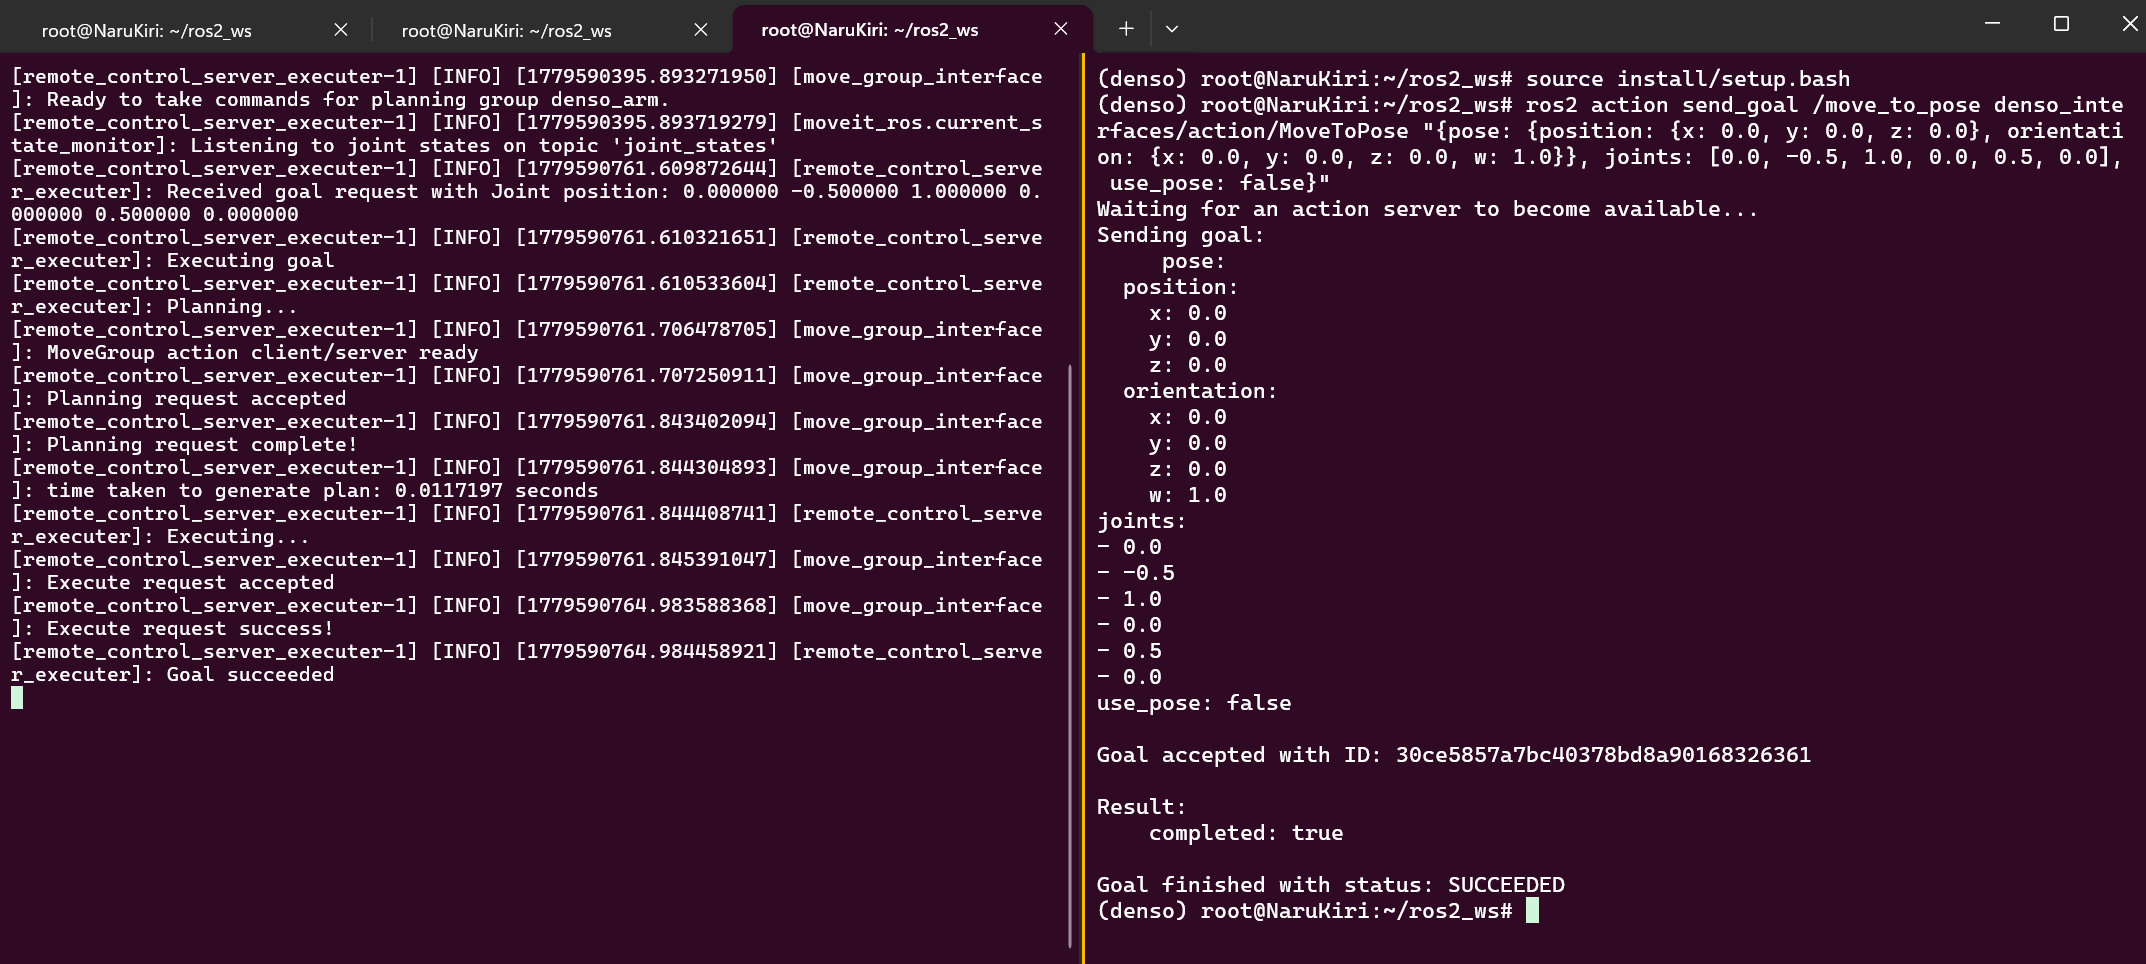
\includegraphics[width=\linewidth]{Images/Implementation/remote_control.png}
        \caption{Denso Remote Control}
    \end{subfigure}
    \hfill
    
    \caption{Các dịch vụ ROS2 chính mà ứng dụng VR truy cập qua RosBridge}
    \label{fig:rosbridge-services}
\end{figure}

Trong đó, \lstinline[style=inlinecode]{/joint_states} từ JointStateBoardcaster dùng để theo dõi trạng thái của cánh tay robot, Denso Remote Control Action Server để điều khiển cánh tay xoay tới vị trí xác định, Denso MoveIt Servo để xoay từng trục của cánh tay liên tục, và hai topic camera từ V4L2 node, để gửi hình ảnh từ camera gửi lên ứng dụng VR.

\section{Ứng dụng VR}

Ở phần này, phần thiết kế và xây dựng ứng dụng VR - module quan trọng thứ 3 của toàn bộ hệ thống, hoàn tất luồng điều khiển từ VR - Ros2 - RC5 của đề tài. Đối với việc xây dựng ứng dụng, đề tài chủ trương sử dụng phiên bản Unity mới nhất - Unity 6, để có thể tận dụng sức mạnh và các tính năng nổi bật từ Game Engine này, cũng như dễ dàng tích hợp với \href{https://developers.meta.com/horizon/downloads/package/meta-xr-sdk-all-in-one-upm/}{Meta XR SDK} để xây dựng ứng dụng VR. Mục tiêu mà ứng dụng VR cần đáp ứng là:
\begin{itemize}
    \item Dễ sử dụng, thân thiện với người dùng.
    \item Hiệu năng ổn định, không crash, FPS không dưới 60.
    \item Tính tương tác cao, đa dạng phương thức điều khiển 
\end{itemize}

\subsection{Chuẩn bị tài nguyên để xây dựng ứng dụng}

Để xây dựng \textbf{ứng dụng VR} điều khiển Robot với\textbf{ Ros2} trên Unity, trước nhất ta phải tiến hành cài đặt hai package quan trọng của ứng dụng, là \href{https://developers.meta.com/horizon/downloads/package/meta-xr-sdk-all-in-one-upm/}{Meta XR SDK} và \href{https://github.com/siemens/ros-sharp}{Ros-Sharp}.

\textbf{Meta XR SDK}

Meta XR SDK là một package lớn và tương đối phức tạp, nên Package này nên được ưu tiên cài đặt trước trên một dự án Unity mới. Chi tiết về cách thức cài đặt trên Unity, từ Import các assets liên quan, thay đổi cấu hình Project, bật hỗ trợ development mode của kính VR... đều được liệt kê rõ, từng bước tại trang \href{https://developers.meta.com/horizon/documentation/unity/unity-tutorial-hello-vr/}{Unity Hello World for Meta Quest VR headsets}

\textbf{Ros-Sharp và Import Robot vào ứng dụng}

Tiếp đến là cài đặt Ros-Sharp package trên Unity, qua đó cho phép giao tiếp với RosBridge Server đã cài đặt trên Ros2 trước đó. Việc cài đặt Ros-sharp cũng tương đối đơn giản, và mặc định package này cũng cung cấp các thao tác cơ bản nhất như kết nối tới Ros2, subscribe/publish vào một vài topic thông dụng của Ros2 cùng một bộ các kiểu dữ liệu Ros2 thông dụng. Điểm ấn tượng của gói package này là cho phép người dùng tự do định nghĩa message/service/action, và cho phép sinh ra các file class phù hợp trong C\# cho các message/service/action này thông qua việc import từ Ros. Tuy nhiên, việc import chỉ hỗ trợ cho việc định nghĩa format message/service/action, còn các hành động như publish, subscribe, gọi Service, gọi Action server và lấy kết quả/feedback... đều cần xây dựng thêm các class cho mỗi hành động, bởi tùy theo cấu trúc của messsage, mà hành động xử lý sẽ khác nhau.

Sau khi cài đặt thành công, người dùng có thể chuyển (transfer) mô hình 3D của robot vào trong Unity thông qua Ros-Sharp. Cách chính xác nhất để "tranfer" là mở một kết nối tới Ros2 đang chạy và đang publish Robot Description, sau đó thực hiện theo hướng dẫn \href{https://github.com/siemens/ros-sharp/wiki/User_App_ROS_TransferURDFFromROS}{TransferURDFFromROS} để đưa Robot vào trong môi trường Unity. Cách làm này đảm bảo mô hình 3D của robot được chuyển qua đầy đủ, kèm toàn bộ những script hỗ trợ đính kèm từng component cho việc đọc dữ liệu \lstinline[style=inlinecode]{\joint_states} để đồng bộ với robot thực tế.

Về phía Ros2, lần lượt chạy các lệnh sau ở hai cửa sổ terminal khác nhau để đảm bảo Robot Description được publish và RosBridge server được khởi động, sẵn sàng để nhận kết nối:

\begin{lstlisting}[style=bashstyle]
    ros2 launch denso_bringup denso_bringup.launch.py
    ros2 launch file_server ros_sharp_communication.launch.py
\end{lstlisting}

Sau đó, ở Unity, ta có thể chỉnh các đường dẫn và tên như sau để import mô hình 3D của robot từ ROS vào Unity

\begin{figure}[H]
    \centering
    \begin{subfigure}{0.48\linewidth}
        \centering
        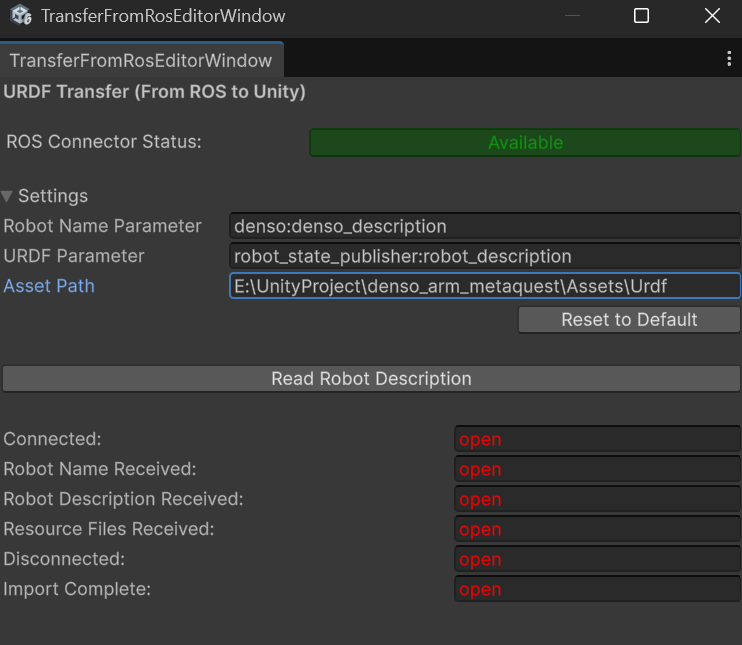
\includegraphics[width=\linewidth]{Images/Implementation/transferfromros.png}
        \caption{Thiết lập Transfer URDF from ROS}
    \end{subfigure}
    \hfill
    \begin{subfigure}{0.48\linewidth}
        \centering
        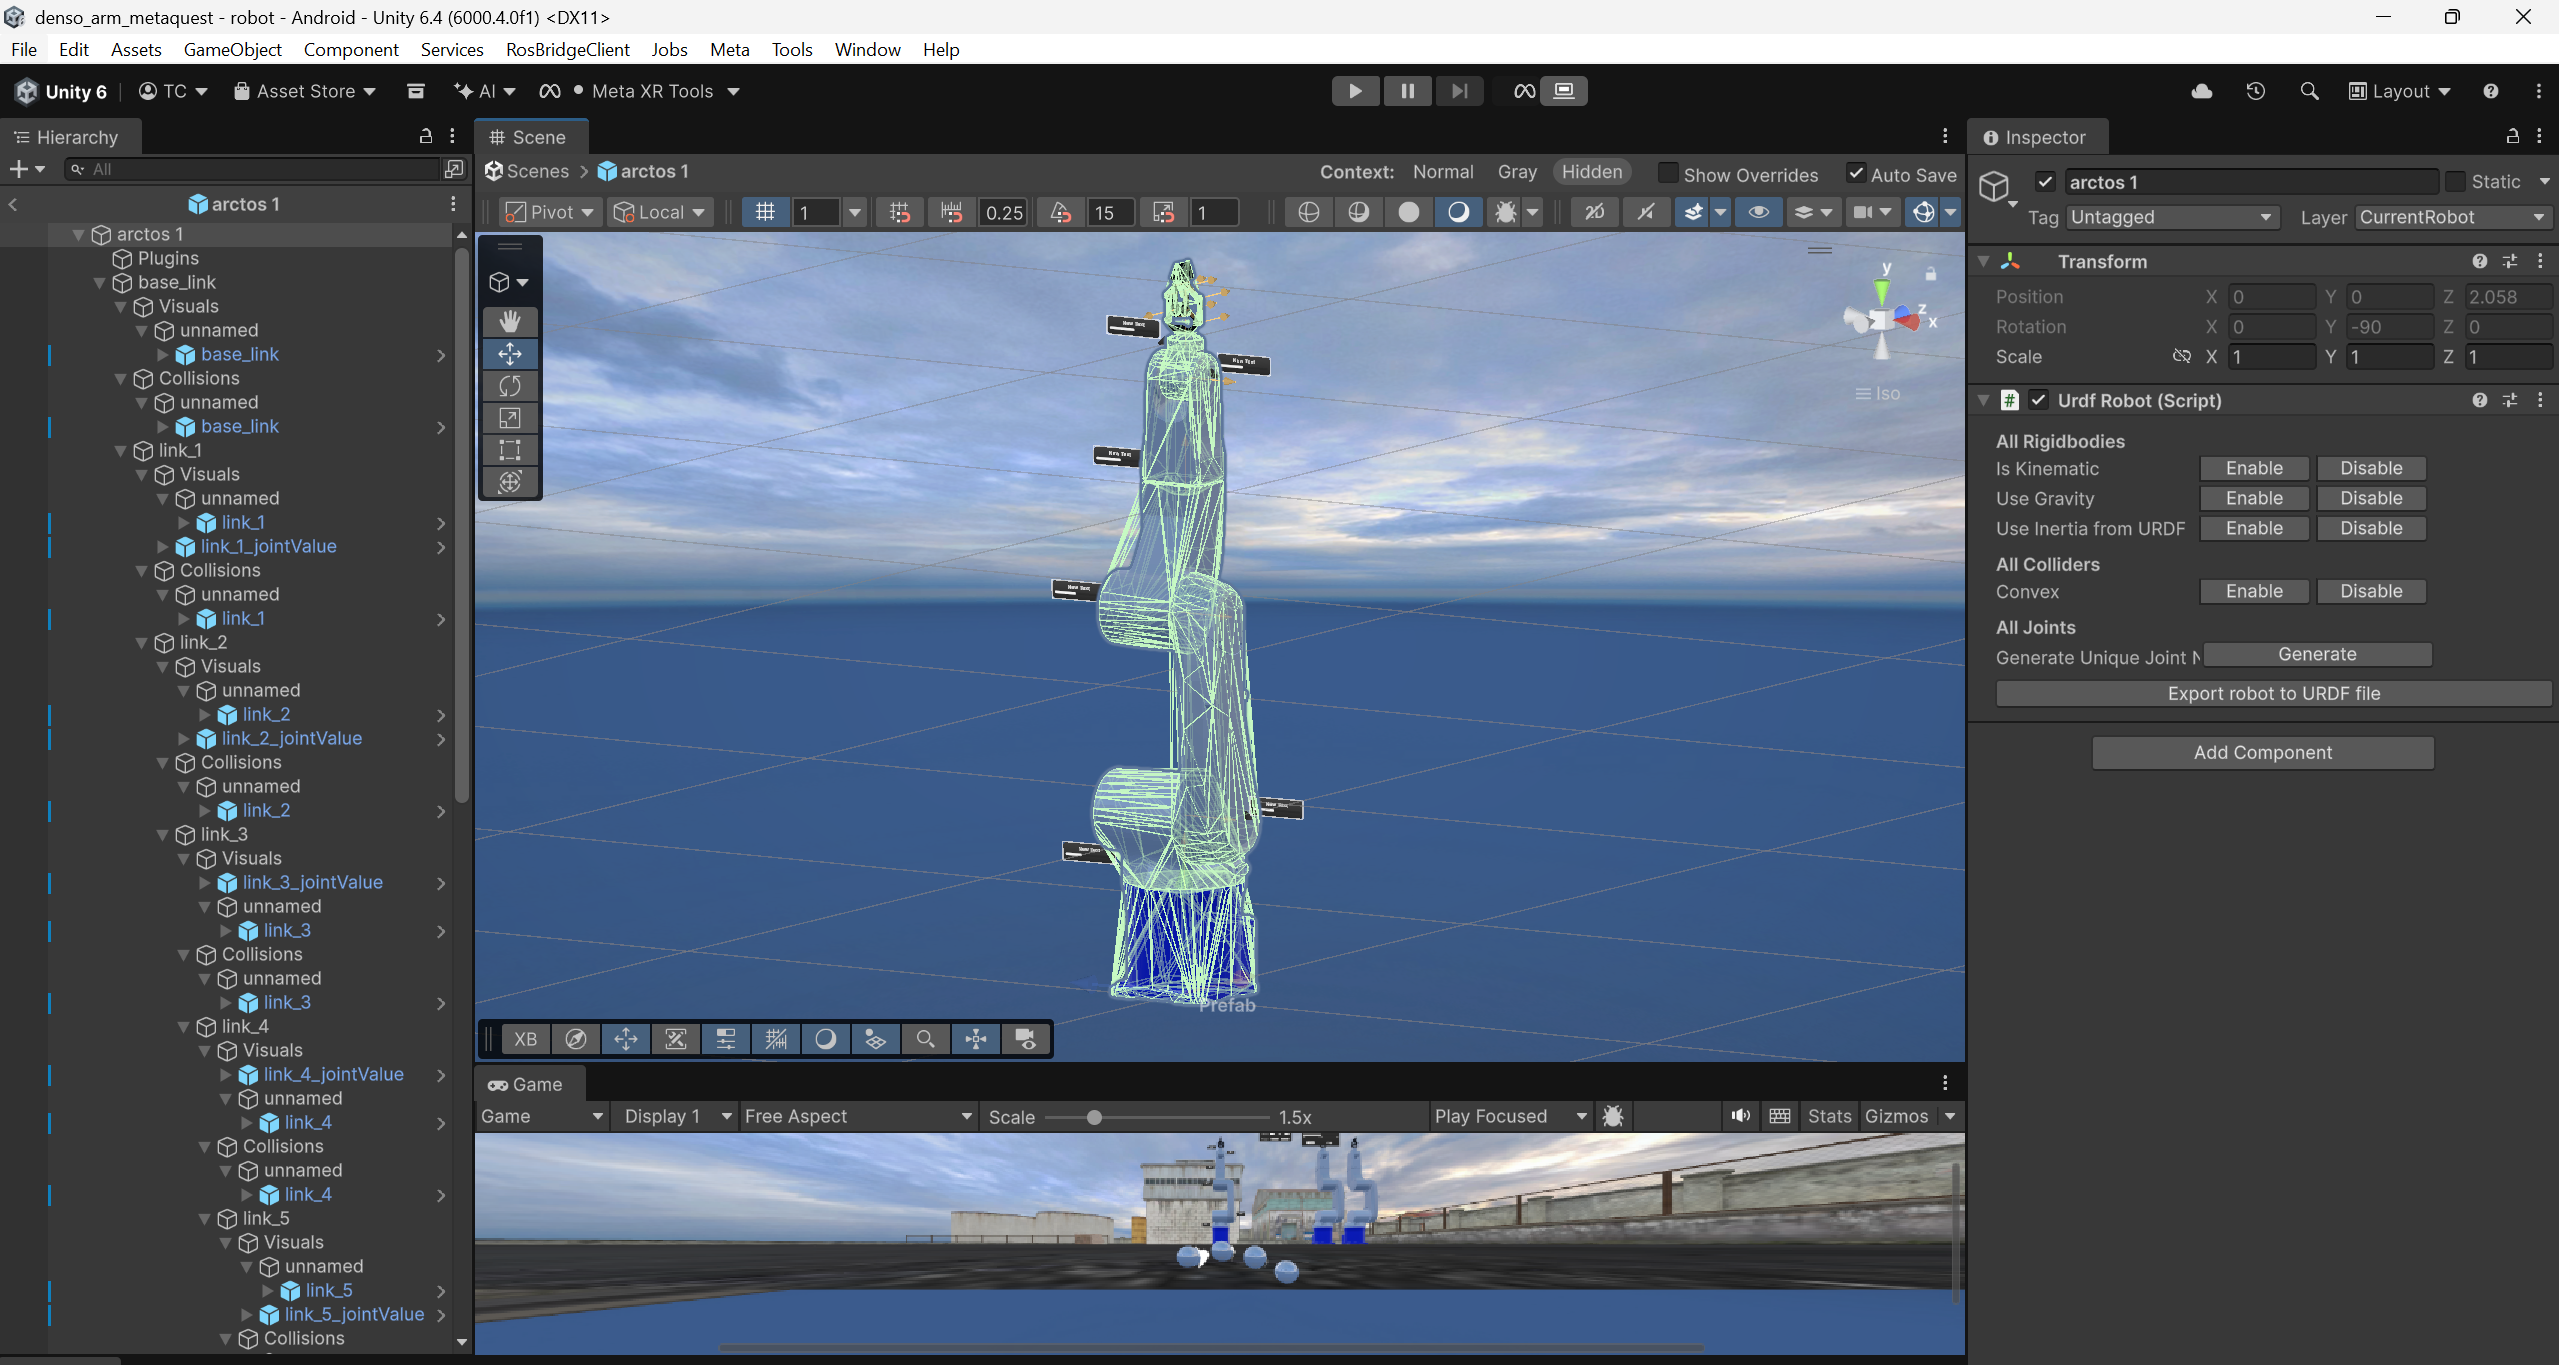
\includegraphics[width=\linewidth]{Images/Implementation/transferfromros_done.png}
        \caption{Kết quả import mô hình robot vào Unity}
    \end{subfigure}
    \caption{Quy trình chuyển mô hình robot từ ROS2 sang Unity}
    \label{fig:transfer-urdf-to-unity}
\end{figure}

\subsection{Kiến trúc phần mềm của ứng dụng VR trên Unity}

Kiến trúc phần mềm cho ứng dụng VR, tương tự cũng sẽ bao gồm hai thành phần chính: Module tương tác VR và Module giao tiếp Ros2. Module tương tác VR chính là phần "giao diện", cho phép người dùng có thể thấy, di chuyển, tương tác với các bảng điều khiển (panel), với Robot, đem lại trải nghiệm khác biệt so với việc sử dụng các công cụ phần mềm 2D, 3D trên máy tính. Module giao tiếp Ros2 đảm nhận phần giao tiếp, được xem là "cốt lõi" của ứng dụng giao tiếp và điều khiển cánh tay Robot thông qua Ros2, và cũng là module được phát triển chủ yếu của đề tài.  

% \\begin{figure}[H]
%     \\centering
%     \\includegraphics[width=0.85\\linewidth]{Images/Implementation/Control/VR_architecture.jpg}
%     \\caption{Kiến trúc tổng quan ứng dụng VR: Module giao tiếp ROS2 và Module tương tác VR}
%     \\label{fig:vr-app-architecture}
% \\end{figure}

\subsection{Module tương tác VR}

Điểm ấn tượng của module Meta XR SDK, đó là được thiết kế để nhà phát triển có thể dễ dàng bắt đầu một dự án VR/AR trên Unity với các "building block" gói gọn những tính năng thông dụng nhất để có thể sử dụng ngay. Thành phần cốt lõi nhất của một ứng dụng sử dụng Meta XR SDK là Camera Rig, với đầy đủ những tính năng như:

\begin{figure}[H]
    \centering
    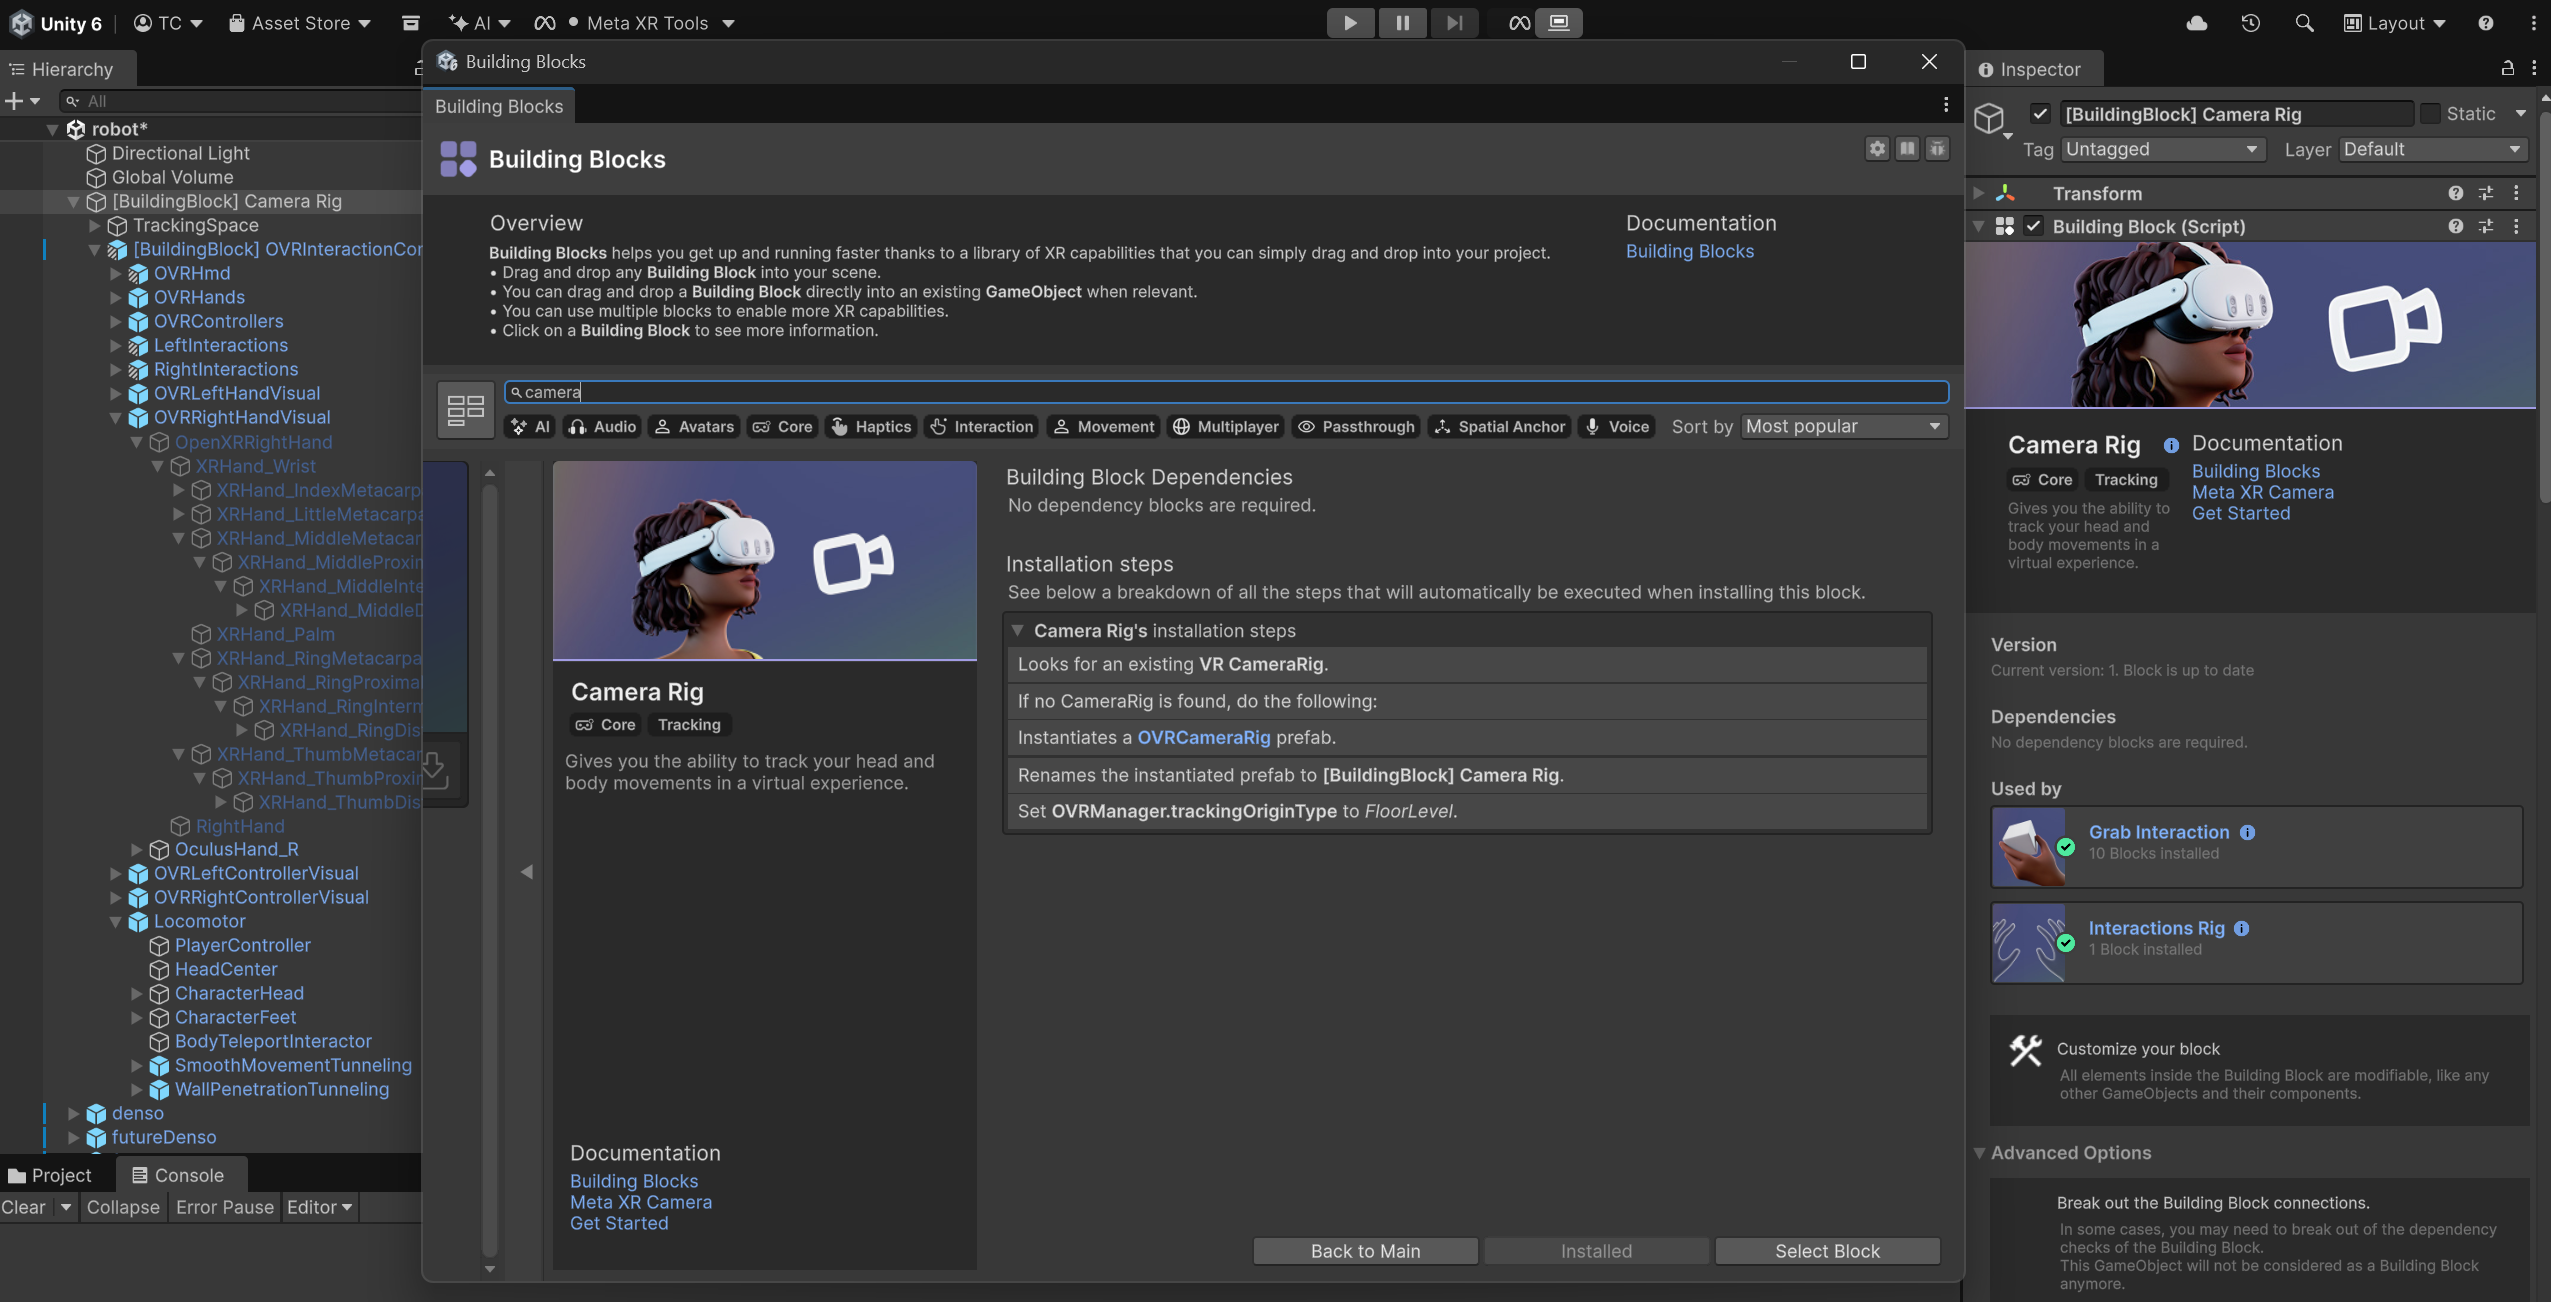
\includegraphics[width=0.7\linewidth]{Images/Implementation/camerarig.png}
    \caption{Camera Rig trong Meta XR SDK}
    \label{fig:camera-rig-meta-sdk}
\end{figure}

\begin{itemize}
    \item Giúp cho người dùng có được góc nhìn trong môi trường VR/AR, hỗ trợ head tracking, eye tracking, cho phép người dùng nhìn xung quanh, xoay đầu trong thế giới ảo
    \item Hỗ trợ di chuyển, xoay nhân vật trong môi trường ảo
    \item Hỗ trợ sử dụng tay cầm, hoặc theo dõi cử động tay và mô phỏng bàn tay trong môi trường ảo. Có thể chuyển từ dạng tay cầm sang mô phỏng bàn tay bằng cách gõ hai tay cầm lại với nhau hai lần. Ngược lại, nhấn nút trên tay cầm sẽ cho phép chuyển từ bày tay mô phỏng sang tay cầm.
    \item Là một "Interactor" giúp đem lại khả năng tương tác với vật thể có thể tương tác được (Interactable).
    \item Cho phép cấu hình nhiều thông số cho việc render hình ảnh trong úng dụng VR, đã được tối ưu với các giá trị khuyên dùng bởi Meta.
\end{itemize}

Việc tương tác được với vật thể cũng là một yếu tố quan trọng cho một ứng dụng VR. Có ba phương pháp để tương tác được hỗ trợ bởi Meta SDK, bao gồm: Poke, Ray và Grab. Các thiết lập cho từng loại tương tác có sự khác biệt đặc trưng:

\begin{itemize}
    \item \textbf{Poke Interactable}: Đây là tương tác cho phép người dùng "Nhấn" lên một đối tượng, thường là nút bấm. Poke Interactable cho phép "nhấn" bằng tay cầm, hoặc dùng ngón tay nếu sử dụng bàn tay mô phỏng. Poke Interatable yêu cầu một Clipped Plane Surface (mặt phẳng cắt) để biết được mặt phẳng mà người dùng sẽ "nhấn" lên.
    \item \textbf{Ray Interactable}: Khi một đối tượng được thêm Ray Interactable, nó cho phép người dùng có thể "trỏ" tới vật thể và tương tác với nó từ xa thông qua tay cầm, hoặc bàn tay mô phỏng. Ray Interactable thường được sử dụng cho giao diện, UI để người dùng có thể nhanh chóng thực hiện thao tác từ xa mà không cần tới gần. Ray Interactable cũng yêu cầu Clipped Plan Surface (mặt phẳng cắt) để biết giới hạn mặt phẳng được trỏ tới.
    \item \textbf{Grab Interactable}: Tương tác nắm có phần phức tạp hơn, và cũng là loại tương tác được dùng phổ biến trong ứng dụng VR. Với Grab Interactable, người dùng có thể cầm nắm vật thể, bằng tay gắp hoặc bàn tay mô phỏng, hỗ trợ nhiều kiểu nắm khác nhau và cho phép di chuyển vật thể trong không gian VR. Để sử dụng Grab Interactable, cần phải sử dụng Building block "Grab Interactable" từ Meta SDK, kèm theo định nghĩa đối tượng là một "Grabbable". Đối tượng cũng cần có "Rigid body" và "Box Collider" để người dùng có thể tác động tới đối tượng và thực hiện hành động nắm.
\end{itemize}

Các Panel điều khiển trong ứng dụng sử dụng cả 3 loại tương tác, và một mô hình 3D "Grab Future Denso Robot" sử dụng Grab Interactable cho phép người dùng tương tác và xoay từng trục của cánh tay một cách trực quan.

\subsection{Module giao tiếp Ros2}

Sơ đồ bên dưới thể hiện kiến trúc tổng quát của module giao tiếp với Ros2 thông qua Web socket. Ros connector là trung tâm của kết nối, một khi khởi tạo và kết nối thành công sẽ cho phép ứng dụng subscribe/publish tới các topic, cũng như sử dụng Service và Action theo nhu cầu. Dữ liệu truyền từ ứng dụng VR sử dụng Ros-Sharp và Ros2 cùng Ros Bridge là các chuỗi JSON theo format message thống nhất.

\subsubsection{Kết nối tới Ros2}

\begin{figure}[H]
    \centering
    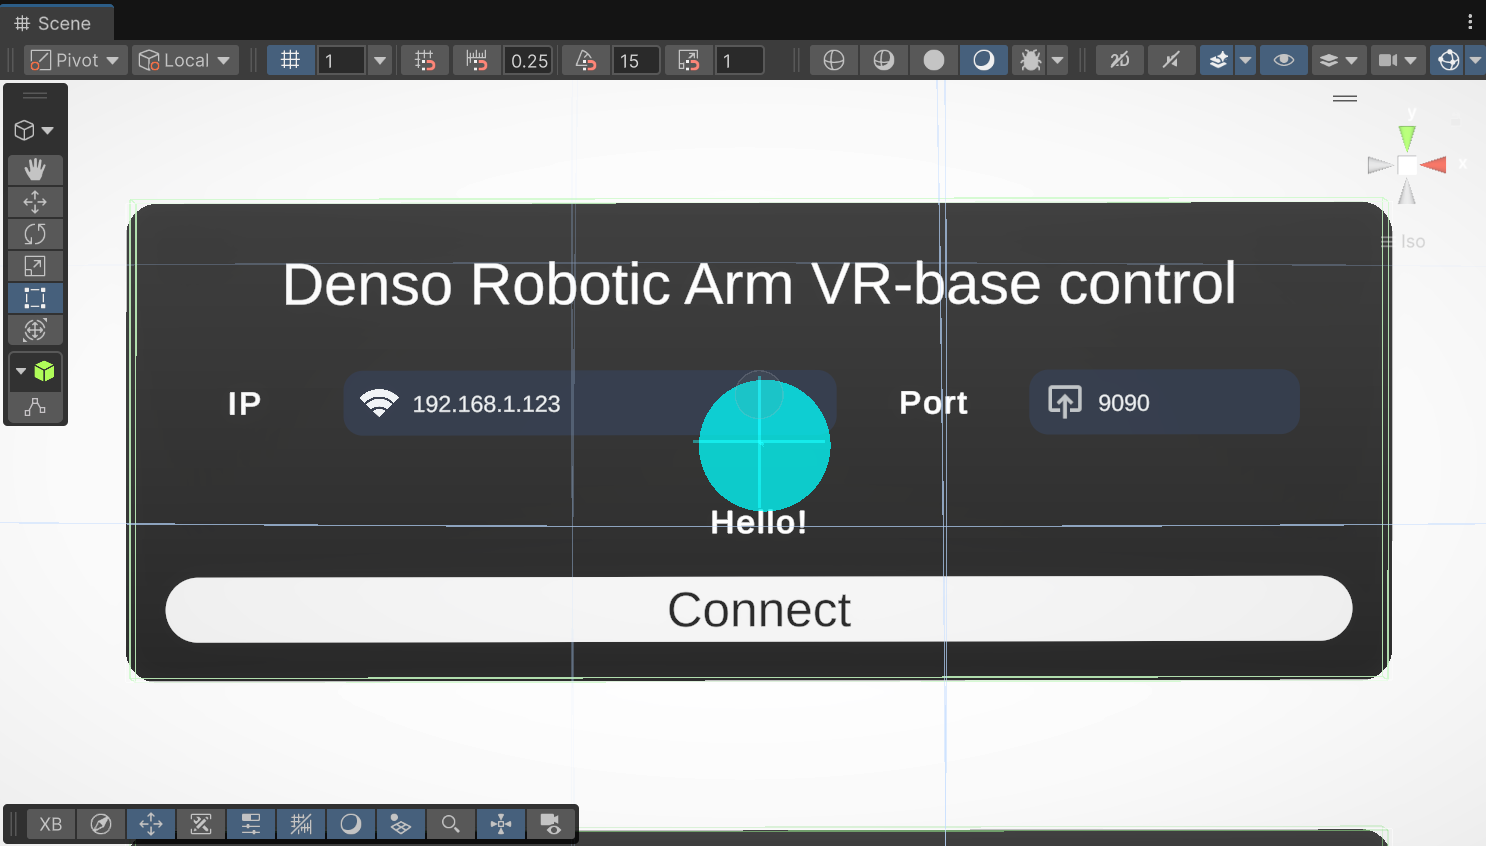
\includegraphics[width=0.75\linewidth]{Images/Implementation/connect_panel.png}
    \caption{Connect Panel và luồng kết nối tới ROS2 qua RosBridge}
    \label{fig:unity-connect-panel}
\end{figure}

Bảng điều khiển để kết nối (connect panel) là điểm khởi đầu cho ứng dụng kết nối. Tại đây, người dùng có thể tương tác với với hai TextField: IP Address và Port để điền vào địa chỉ của máy đang chạy Ros2 cùng RosBridge Server và tạo kết nối tới port đã chọn. Giá trị port ở đây sẽ là 9090, như đã cấu hình cho RosBridge Server ở phía máy PC chạy Ros2. 

Sau khi nhập địa chỉ, nhấn nút Connect để bắt đầu kết nối tới Ros2. Module "Connect to Ros2 Manager" đảm nhận việc thu thập giá trị IP và port đã định nghĩa và khởi tạo kết nối tới Ros2. Trạng thái của kết nối sẽ được hiển thị trực quan ngay trên nút kết nối. 

Khi kết nối thành công, các panel điều khiển khác sẽ hiện ra đầy đủ, cho phép người dùng tiến hành điều khiển cánh tay robot thông qua VR. Ngược lại, khi không còn sử dụng, người dùng có thể nhấn nút Disconnect để hủy kết nối tới Ros2, và các bảng điều khiển cũng sẽ tắt đi tương ứng.

\subsubsection{Theo dõi Camera với Image subscription}

Khi kết nối thành công tới PC chạy Ros2, các dịch vụ phụ thuộc vào Ros2 Connector sẽ tự động khởi chạy theo, trong đó có Compressed Image Subscriber, có nhiệm vụ subscribe vào topic hình ảnh nén (compressed image) từ Ros2. 

\begin{figure}[H]
    \centering
    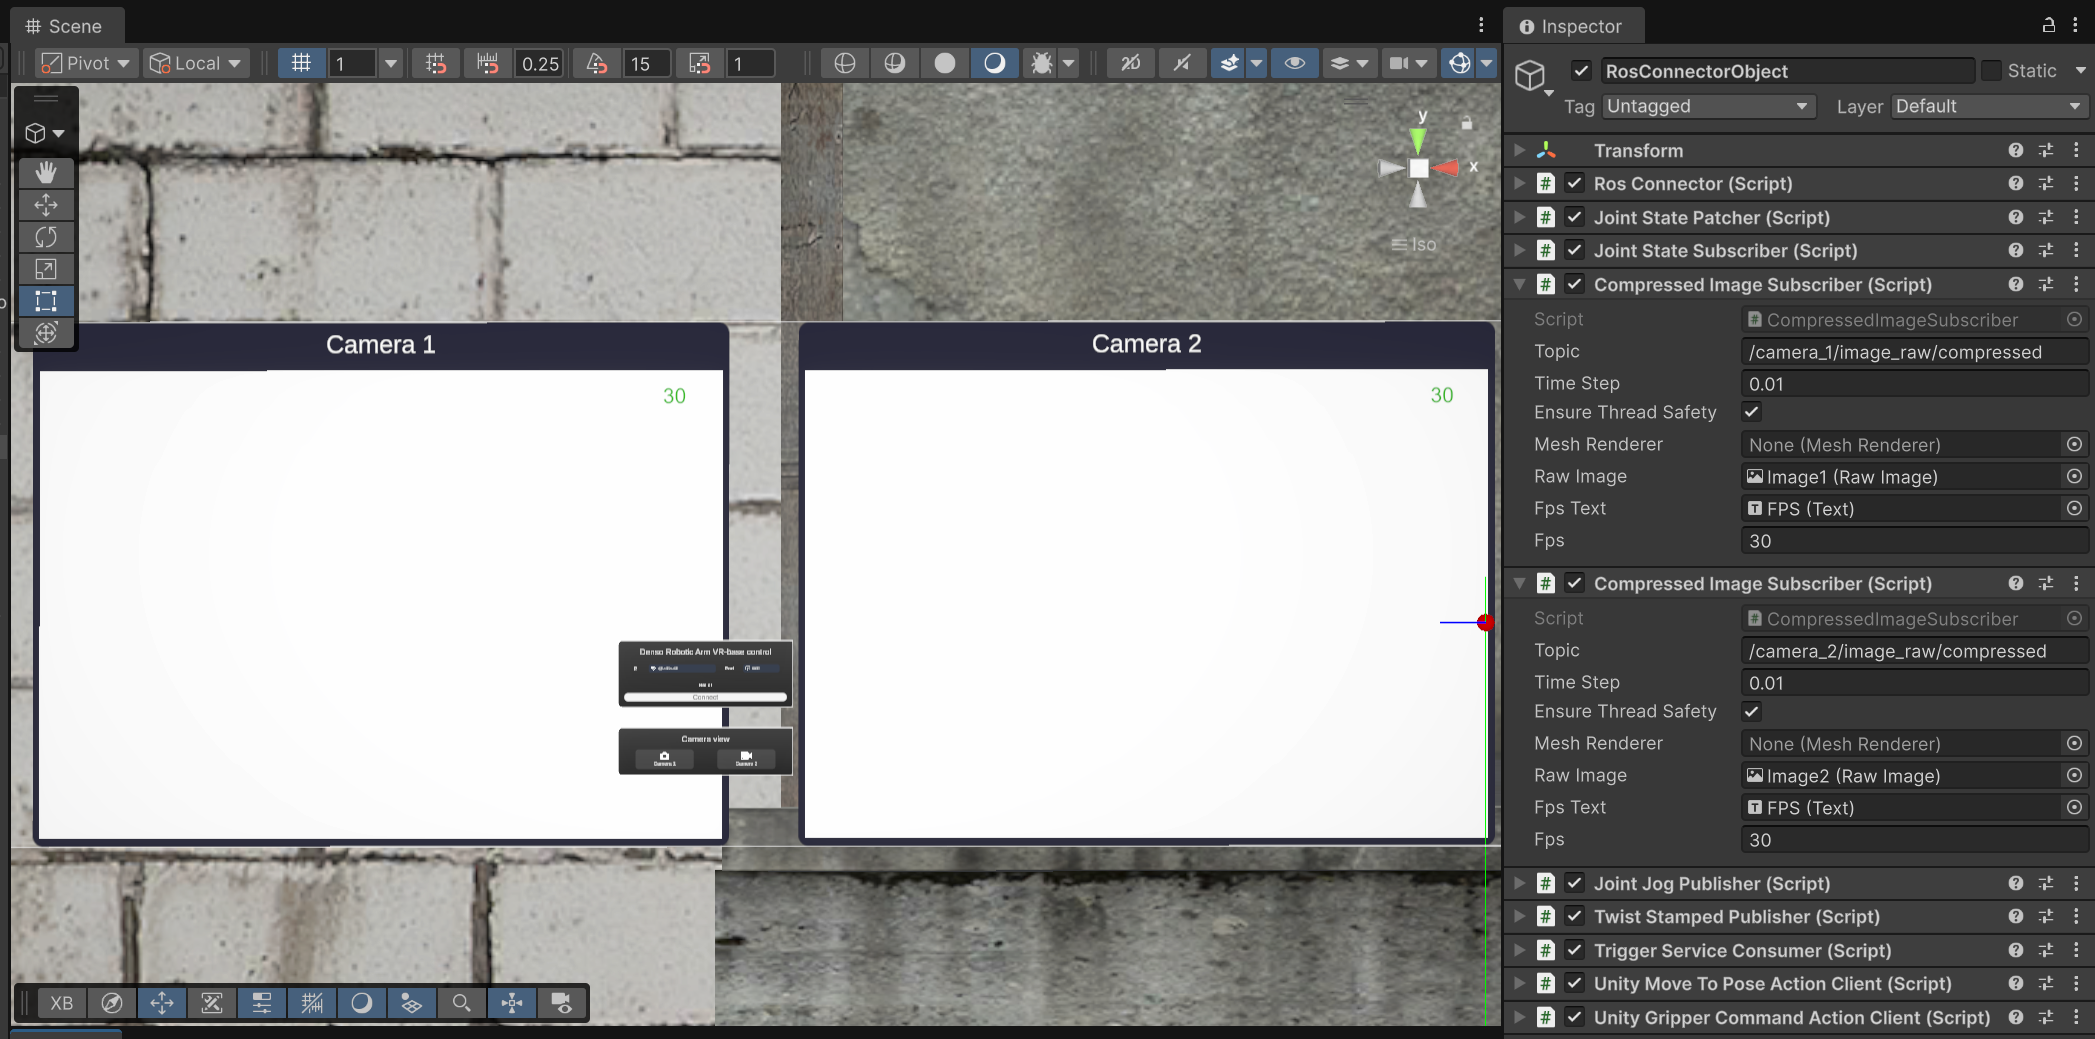
\includegraphics[width=0.72\linewidth]{Images/Implementation/image_subscriber.png}
    \caption{Cấu hình Compressed Image Subscriber trong Unity}
    \label{fig:image-subscriber-unity}
\end{figure}

Do nhu cầu sử dụng hai camera, sẽ có hai Compressed Image Subscriber được sử dụng, mỗi một subscriber truy cập tới một topic. Thuộc tính "Time Step" cho biết Subscriber sẽ xét dữ liệu mới mỗi 0.01s, hay 10ms. Khi có dữ liệu mới, hàm \lstinline[style=inlinecode]{ReceiveMessage()} của script này sẽ được gọi kèm dữ liệu ảnh. Dữ liệu ảnh được chuyển thành Texture2D ngay sau đó, và hiển thị lên "Raw Image". Ngoài ra, Script cũng hỗ trợ thu thập giá trị FPS ảnh thu được, cụ thể là một đối tượng Text ở góc phải trên của mỗi màn hình camera.

\subsubsection{Theo dõi trạng thái Robot thực tế thông qua Joint State subscription}

Để theo dõi trạng thái của cánh tay thực tế, Joint State Subscriber được sử dụng để subscribe vào topic \lstinline[style=inlinecode]{/joint\_states} nhằm theo dõi vị trí các trục robot được gửi ra từ Robot State Publisher. Joint Names là một mảng mà ta có thể ghi rõ tên của các trục cần theo dõi giá trị vị trí (hay góc) ở từng phần tử (Element). Joint State Writer của Element tương ứng sẽ được sử dụng để trực tiếp xoay trục của cánh tay robot với giá trị góc nhận được, từ đó hiện thực cơ chế đồng bộ giữa mô hình Denso Robot và trạng thái cánh tay robot thực tế được gửi ra từ Ros2. 

% \begin{figure}[H]
%     \centering
%     \includegraphics[width=0.72\linewidth]{Images/Implementation/Control/DensoHand_Read_flow.jpg}
%     \caption{Cấu hình Joint State Subscriber}
%     \label{fig:joint-state-subscriber-unity}
% \end{figure}

Đối với phần tay gắp, do đây là loại tay gắp song song (parallel gripper), nên cấu hình robot từ Ros2 sẽ chỉ có duy nhất một trục của tay gắp được truyền là trục bên phải (gripper\_gear\_right\_joint). Để tạo cơ chế điều khiển cả hai trục trái và phải của mô hình 3D trong ứng dụng VR, script đã được tùy chỉnh để hỗ trợ mirror joint (trục ánh xạ), bằng cách dùng chung tên cho phần Joint names, và phần Joint state Writer sẽ là hai trục trái và phải. 

\subsubsection{Điều khiển robot với MoveIt Servo}

Khi nói đến ứng dụng điều khiển cánh tay robot, nhu cầu đầu tiên sẽ là điều khiển từng trục của robot xoay trực tiếp. MoveIt-Servo Panel hỗ trợ nhu cầu này, bằng cách cho phép người dùng kích hoạt tính năng MoveIt-Servo từ Ros2, sau đó gửi lệnh xoay trục (JointJog) hoặc xoay tọa độ (Twist Stamped) tới MoveIt-Servo. Panel có thiết kế giao diện như sau:

\begin{figure}[H]
    \centering
    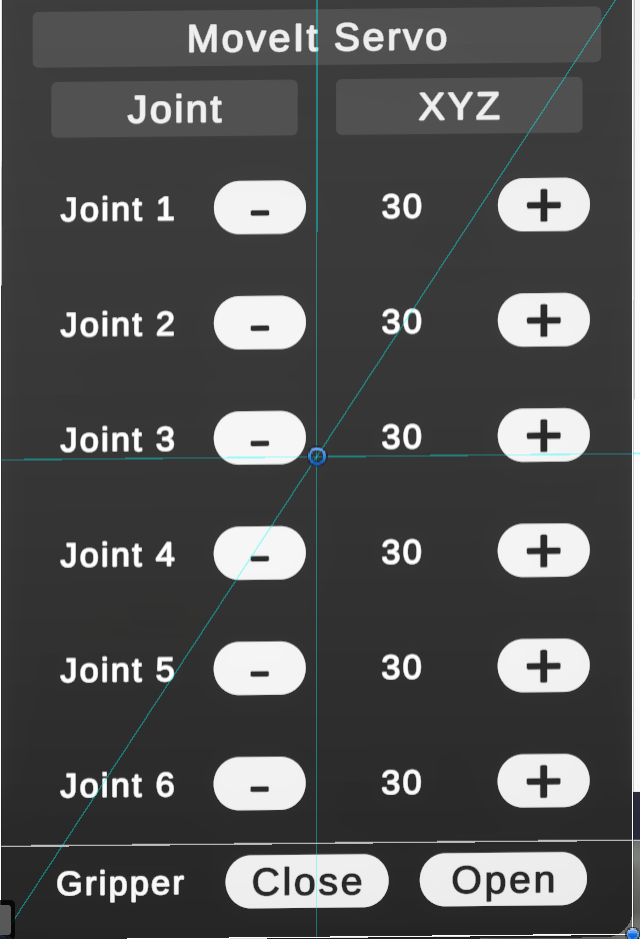
\includegraphics[width=0.72\linewidth]{Images/Implementation/moveit_servo_panel.png}
    \caption{Giao diện MoveIt-Servo Panel trong ứng dụng VR}
    \label{fig:moveit-servo-panel-unity}
\end{figure}

Đầu tiên, người dùng cần phải kích hoạt tính năng MoveIt-Servo, bằng cách gửi một Trigger Service request tới Denso MoveIt Servo node chạy trên PC Ros2. Hỗ trợ cho tính năng này, UnityServiceConsumer và TriggerServiceConsumer được xây dựng, với UnityServiceConsumer là một abstract class chung cho Serivce, và TriggerServiceConsumer cung cấp phương thức gửi Service request và nhận Service response cho một loại service (Trigger).

Service Request dạng Trigger được gửi tới Ros2 cho việc bật/tắt MoveIt-Servo là:

\begin{itemize}
    \item \textbf{Bật MoveIt-Servo:} \lstinline[style=inlinecode]{/denso_moveit_servo_node/start_servo}
    \item \textbf{Tắt MoveIt-Servo:} \lstinline[style=inlinecode]{/denso_moveit_servo_node/stop_servo}
\end{itemize}

Sau khi bật MoveIt-Servo, người dùng có thể tiếp tục thực hiện điều khiển xoay từng trục trong 6 trục (Chế độ Joint) hoặc xoay theo tọa độ (Chế độ XYZ). JointJogPublisher được dùng để publish JointJog message tới topic \lstinline[style=inlinecode]{/denso_moveit_servo_node/delta_joint_cmds}, và TwistStampedPublisher publish TwistStamped message vào topic \lstinline[style=inlinecode]{/denso_moveit_servo_node/delta_twist_cmds}. Để điều khiển, người dùng chỉ cần nhấn vào nút "+" hoặc nút "-" của từng trục để thực hiện gửi lệnh điều khiển tăng/giảm góc tới trục tương ứng, tương tự với việc thay đổi tọa độ XYZ.

Ngoài ra, ở mỗi hàng điều khiển trục, con số ở giữa cho biết giá trị góc của trục hiện tại, lấy từ nhiều "Joint State Reader" được đặt ở từng trục trong mô hình Denso Robot, để người dùng thấy được chính xác giá trị góc của robot trong quá trình điều khiển.

\subsubsection{Đóng mở Gripper với GripperCommand Action Client}

Trong MoveIt-Servo panel, ngoài tính năng điều khiển bằng MoveIt-Servo, ta còn có hai nút nhấn để thực hiện đóng/ mở tay gắp. Đối với controller của tay gắp được hiện thực ở phía Ros2 (denso\_hand\_controller - loại GripperActionController), do đây là loại controller đơn giản và cách điều khiển không cần quá phức tạp, đề tài chủ trương giao tiếp trực tiếp với Action Server của controller cho tay gắp, thông qua việc tạo Action client loại GripperCommand.

Trước khi hiện thực GripperCommand Action Client, ta cần định nghĩa class Action phù hợp trong Unity. Package Ros-Sharp hỗ trợ điều này thông qua tính năng Generate Action trong RosBridgeClient -> Auto Generate Action -> Single Action, và trỏ tới file action tương ứng:

\begin{figure}[H]
    \centering
    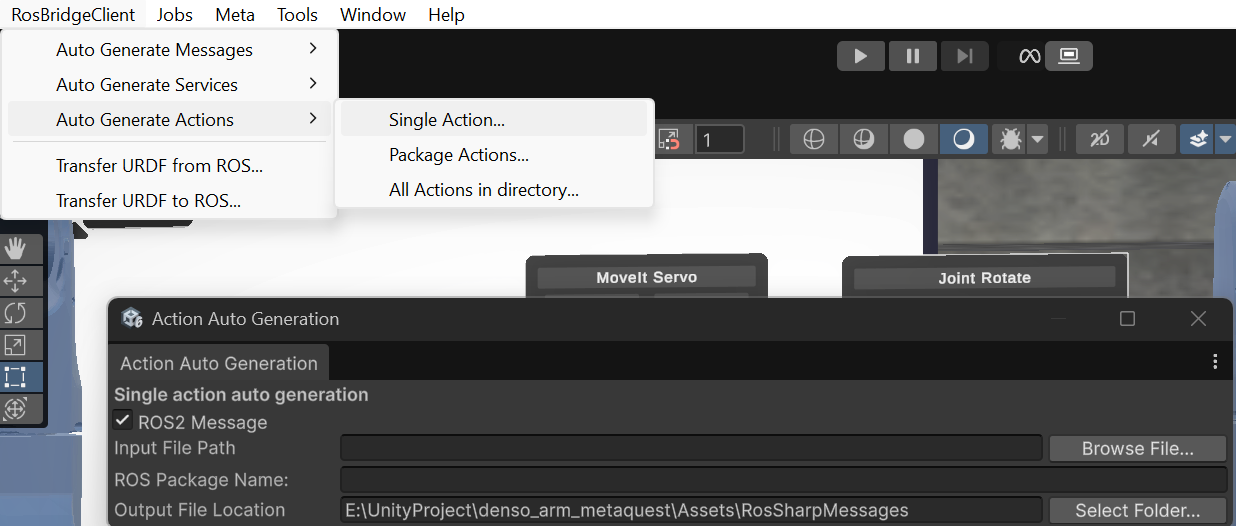
\includegraphics[width=0.75\linewidth]{Images/Implementation/generate_action.png}
    \caption{Tạo Action class trong Ros-Sharp từ file action của ROS2}
    \label{fig:generate-action-rossharp}
\end{figure}

Ros-Sharp sẽ tự động generate cho GripperCommand bảy class cho Action này, bao gồm:

\begin{enumerate}
    \item GripperCommandAction
    \item GripperCommandActionFeedback
    \item GripperCommandActionGoal
    \item GripperCommandActionResult
    \item GripperCommandFeedback
    \item GripperCommandGoal
    \item GripperCommandResult
\end{enumerate}

Tiếp đến, class GripperCommandActionClient được hiện thực, kế thừa từ class ActionClient với toàn bộ bảy class của Action GripperCommand được xây dựng, cung cấp những API cơ bản như \lstinline[style=inlinecode]{SetActionGoal(), OnFeedbackReceived(), OnResultReceived()} để gửi Goal, theo dõi feedback và sau cùng là nhận result, như một Action client cơ bản của Ros2.

Dựa trên class GripperCommandActionClient, UnityGripperCommandActionClient kế thừa MonoBehavior để phù hợp trong môi trường Unity, khởi tạo chính thức một object GripperCommandActionClient để có thể gửi lệnh đóng hoặc mở Gripper, đồng thời theo dõi feedback và result ở hàm \lstinline[style=inlinecode]{Update()} của Unity.

\begin{figure}[H]
    \centering
    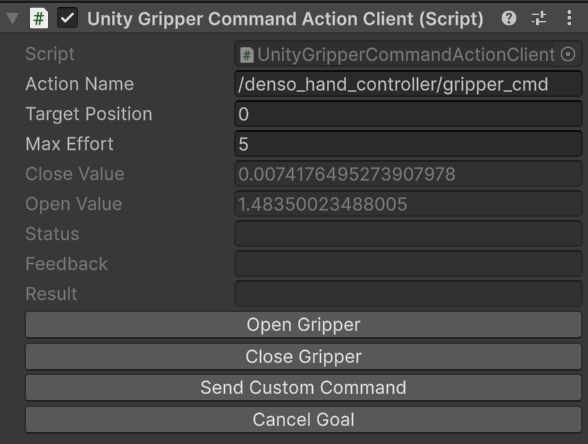
\includegraphics[width=0.75\linewidth]{Images/Implementation/unitygrippercommand.png}
    \caption{Hiện thực UnityGripperCommandActionClient}
    \label{fig:unity-gripper-command-client}
\end{figure}

\subsubsection{Điều khiển robot với MoveToPose Action Client}

MoveToPose là một custom action, dành riêng cho Denso Remote Control Action Server được hiện thực ở phần Ros2, nhằm mục tiêu gửi lệnh điều khiển robot xoay tới vị trí mong muốn thông qua giá trị góc trục hoặc tọa độ XYZ. Vì là một custom action, ta buộc phải import bộ action này vào Unity bằng tính năng Generate Action, tương tự như với Gripper Command. Bộ file được sinh ra sẽ bao gồm:

\begin{enumerate}
    \item MoveToPoseAction
    \item MoveToPoseActionFeedback
    \item MoveToPoseActionGoal
    \item MoveToPoseActionResult
    \item MoveToPoseFeedback
    \item MoveToPoseGoal
    \item MoveToPoseResult
\end{enumerate}

Class MoveToPoseActionClient được hiện thực kế thừa class ActionClient cùng bảy class của MoveToPose phía trên, chung nhiệm vụ cung cấp các API cơ bản để có thể gửi Goal, nhận feedback và result. Trên lớp MoveToPoseActionClient, UnityMoveToPoseActionClient là class được sử dụng chính: tạo object MoveToPoseActionClient nhằm tạo goal, gửi goal và liên tục lấy các kết quả. 

Điểm quan trọng trong hiện thực của MoveToPose Action Client, đó là cho phép tạo goal bằng danh sách các Joint và cả goal bằng tọa độ XYZ, tuy nhiên cơ chế điều khiển bằng tọa độ chưa có độ tin cậy tốt, bởi một giá trị tọa độ có thể có rất nhiều giá trị trục có thể thỏa mãn vị trí đó (động học nghịch), dẫn tới robot có thể được MoveIt2 planning và execute với "Pose" - hay dáng của robot không đúng như mong đợi. Cơ chế điều khiển bằng tọa độ XYZ hiện tại cần nhiều thời gian để nghiên cứu hơn, do đó chưa áp dụng cho ứng dụng điều khiển hiện tại.

Vì giới hạn trên, cơ chế điều khiển thông qua giá trị 6 trục Robot được sử dụng chủ yếu. Đối với cơ chế này, ứng dụng cung cấp hai phương thức điều khiển: Xoay trục bằng bảng điều khiển và tương tác với cánh tay để xoay.

\textbf{Xoay Robot với bảng điều khiển}

Cách thức "Xoay robot với bảng điều khiển" lấy cảm hứng dựa theo ứng dụng Rviz trên Ros2, khi người dùng được phép sử dụng các thanh ngang để xoay mô hình robot tương lai "Goal State" và xem xét hình dáng, trạng thái của cánh tay robot, trước khi thực hiện Planning và Execute. Đối với cách thức này, người dùng sẽ nhấn chọn nút Joint Rotate trên bảng điều khiển để chuyển sang mode điều khiển bằng cách xoay các slider. Các slider sẽ hiện ra, cùng với một bản sao mô hình 3D của robot Denso, gọi là "Future Denso Robot". Bản sao robot này được điều khiển hoàn toàn bởi Joint Rotate Panel, tức giá trị của slider sẽ tương ứng với giá trị của mỗi trục cánh tay. 

\begin{figure}[H]
    \centering
    \begin{subfigure}{0.48\linewidth}
        \centering
        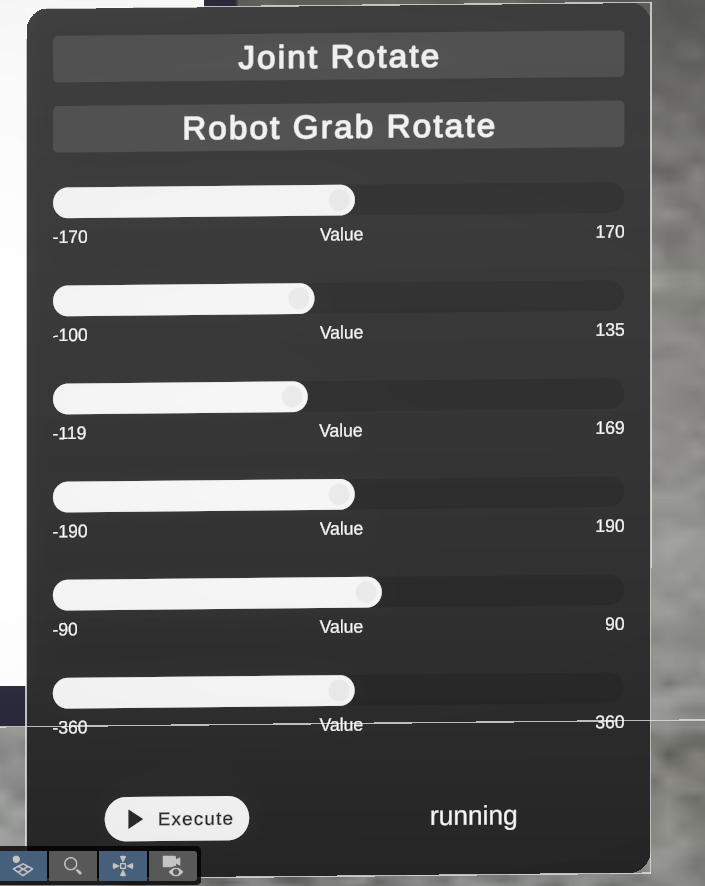
\includegraphics[width=\linewidth]{Images/Implementation/jointrotate.png}
        \caption{Joint Rotate Panel}
    \end{subfigure}
    \hfill
    \begin{subfigure}{0.48\linewidth}
        \centering
        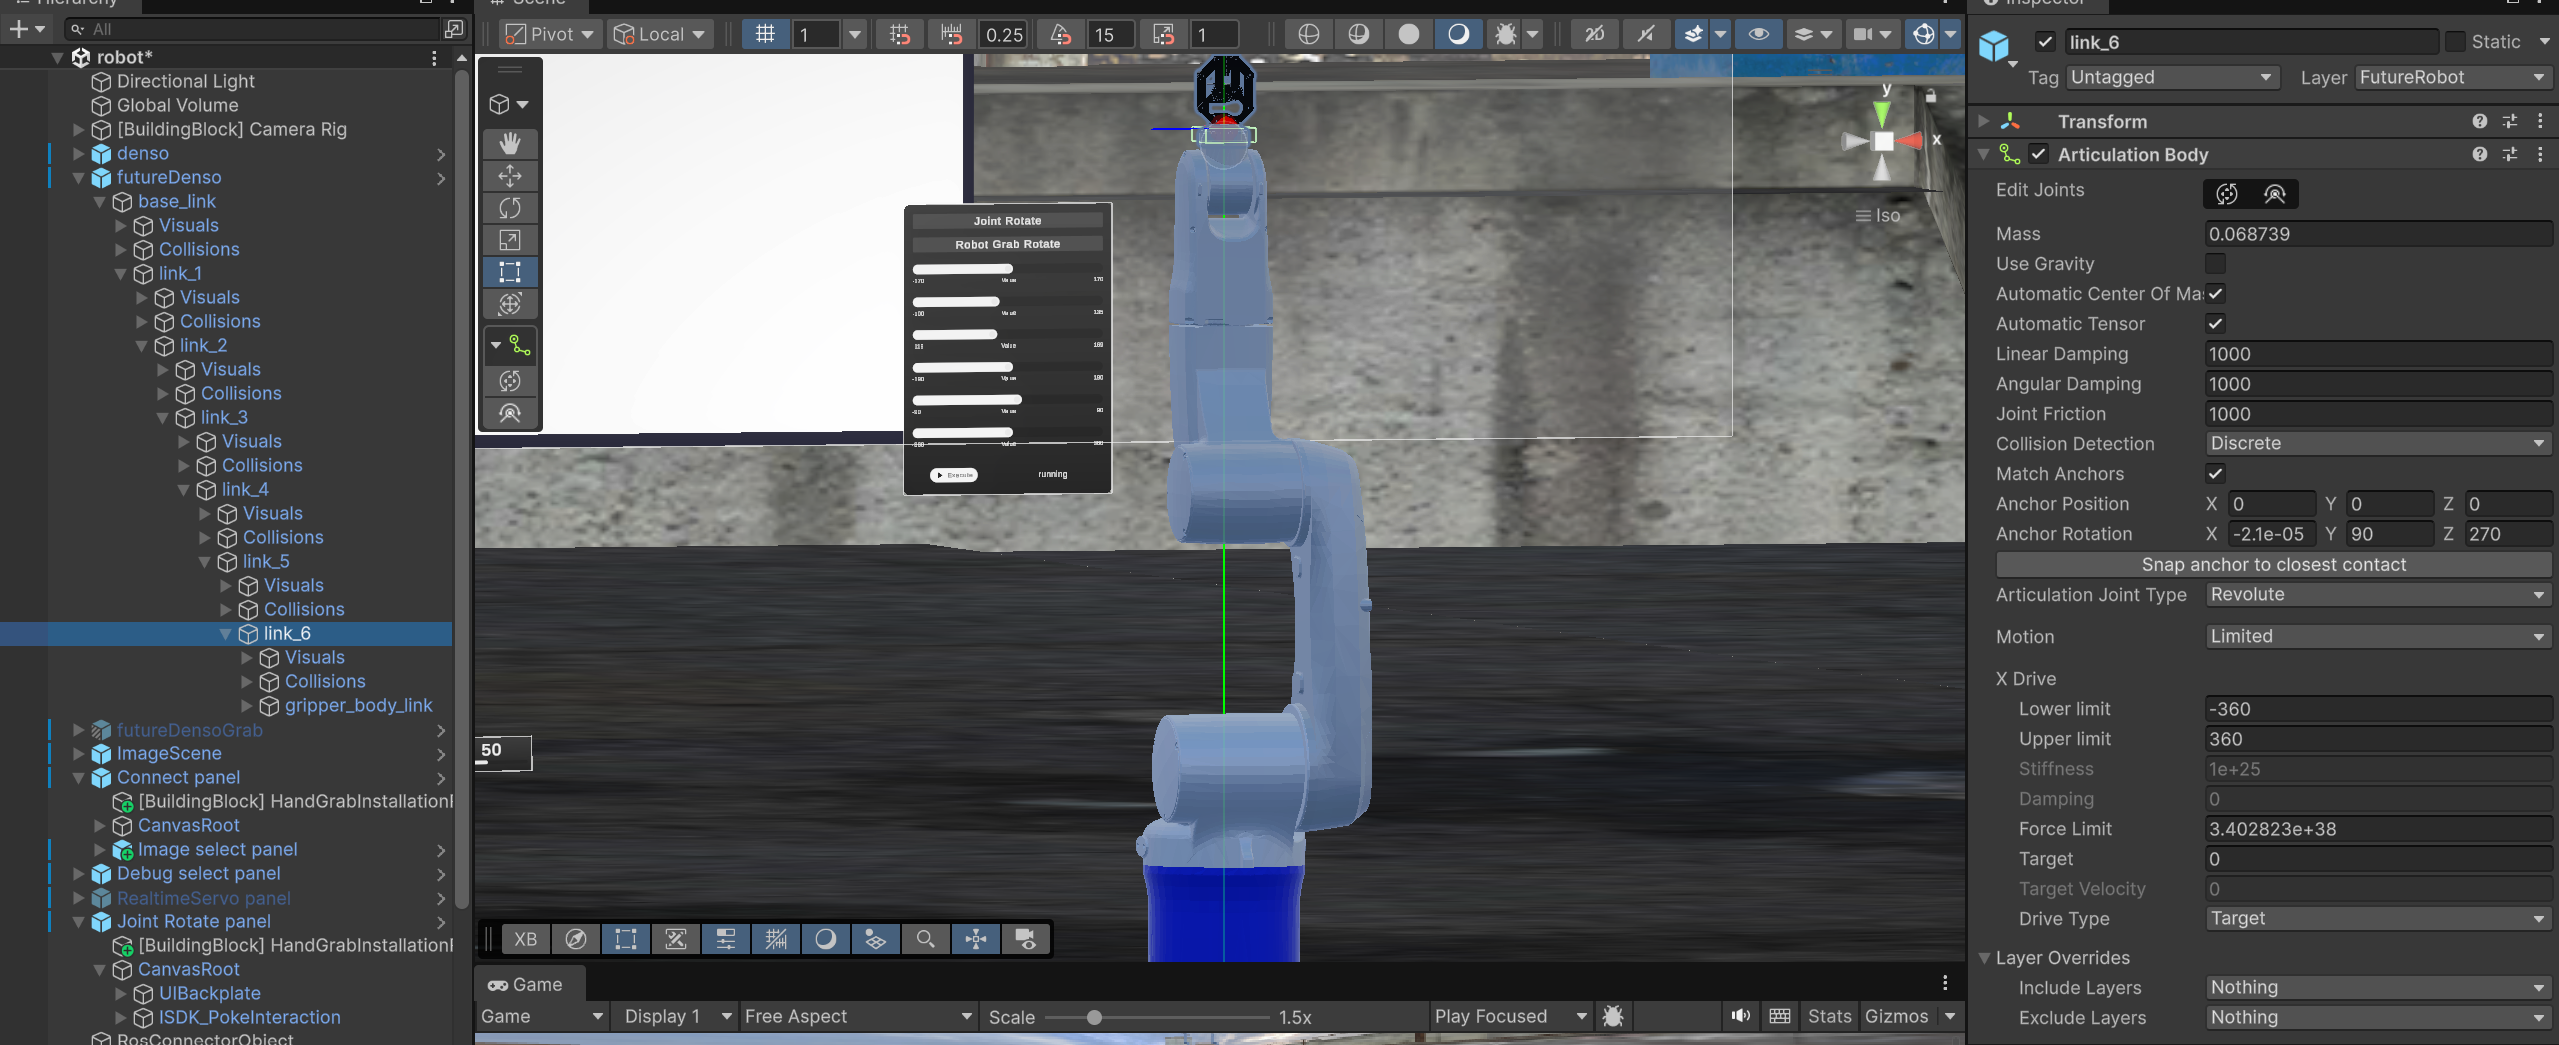
\includegraphics[width=\linewidth]{Images/Implementation/futuredenso_articulation.png}
        \caption{Future Denso Robot với Articulation Body}
    \end{subfigure}
    \caption{Điều khiển robot bằng bảng điều khiển và mô hình Future Denso Robot}
    \label{fig:joint-rotate-and-future-robot}
\end{figure}

Để đảm bảo mô hình 3D Future Denso Robot xoay mượt và ổn định, đề tài sử dụng các Articulation Body cho các trục thay vì chỉ sử dụng bộ Rigid Body + Hinge Joint để mô tả một khớp xoay tròn, kèm theo giới hạn xoay để tránh trường hợp xoay quá giá trị cho phép ở từng trục.

Sau khi đã xoay robot tới vị trí mong muốn bằng slider, nhấn nút Execute sẽ lần lượt thực hiện các bước sau:

\begin{itemize}
    \item Các giá trị góc ở từng slider được thu thập và tạo thành một List chứa giá trị góc mong muốn cho từng trục
    \item Tạo MoveToPose Goal với danh sách các trục, usePose = false.
    \item Goal được gửi tới thiết bị Ros2 thông qua UnityMoveToPoseActionClient
\end{itemize}

Khi Action Goal của MoveToPose được gửi, Action Server ở phía Ros2 sẽ nhận Goal, kiểm tra tính hợp lệ của lệnh và thực hiện Planning + Execute cánh tay tương ứng bằng MoveIt2. Trong quá trình xoay cánh tay, trạng thái của cánh tay sẽ luôn được cập nhật liên tục nhờ hoạt động của Joint State Subscriber, từ đó điều khiển mô hình chính - "Denso robot" xoay tương ứng, cho biết chính xác trạng thái thực tế của cánh tay. Quá trình Execute hoàn tất khi MoveIt2 đưa cánh tay tới vị trí tương đồng như vị trí cánh tay đã chỉnh thông qua cách bảng điều khiển bằng Slider.

\textbf{Xoay Robot bằng cách tương tác với mô hình}

Đây là cách điều khiển trực quan hơn so với việc sử dụng Slider, cho phép người dùng thật sự tương tác với model cánh tay robot. Để kích hoạt chức năng này, người dùng bấm vào nút Robot Grab Rotate để chuyển sang cách điều khiển tương tác mô hình. Giao diện của bảng điều khiển sẽ chuyển sang như hình dưới:

\begin{figure}[H]
    \centering
    \begin{subfigure}{0.48\linewidth}
        \centering
        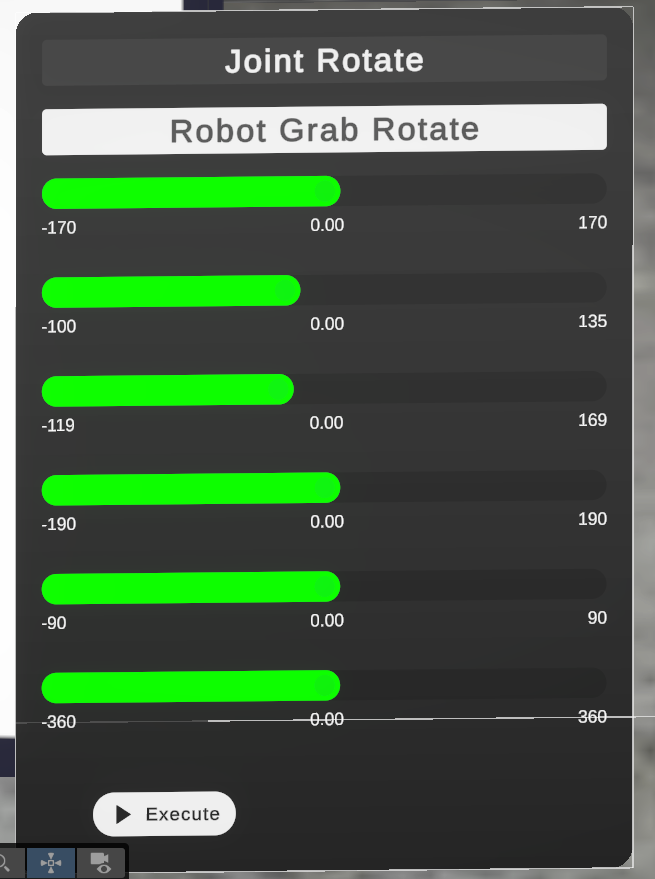
\includegraphics[width=\linewidth]{Images/Implementation/robotgrabrotate.png}
        \caption{Giao diện Robot Grab Rotate}
    \end{subfigure}
    \hfill
    \begin{subfigure}{0.48\linewidth}
        \centering
        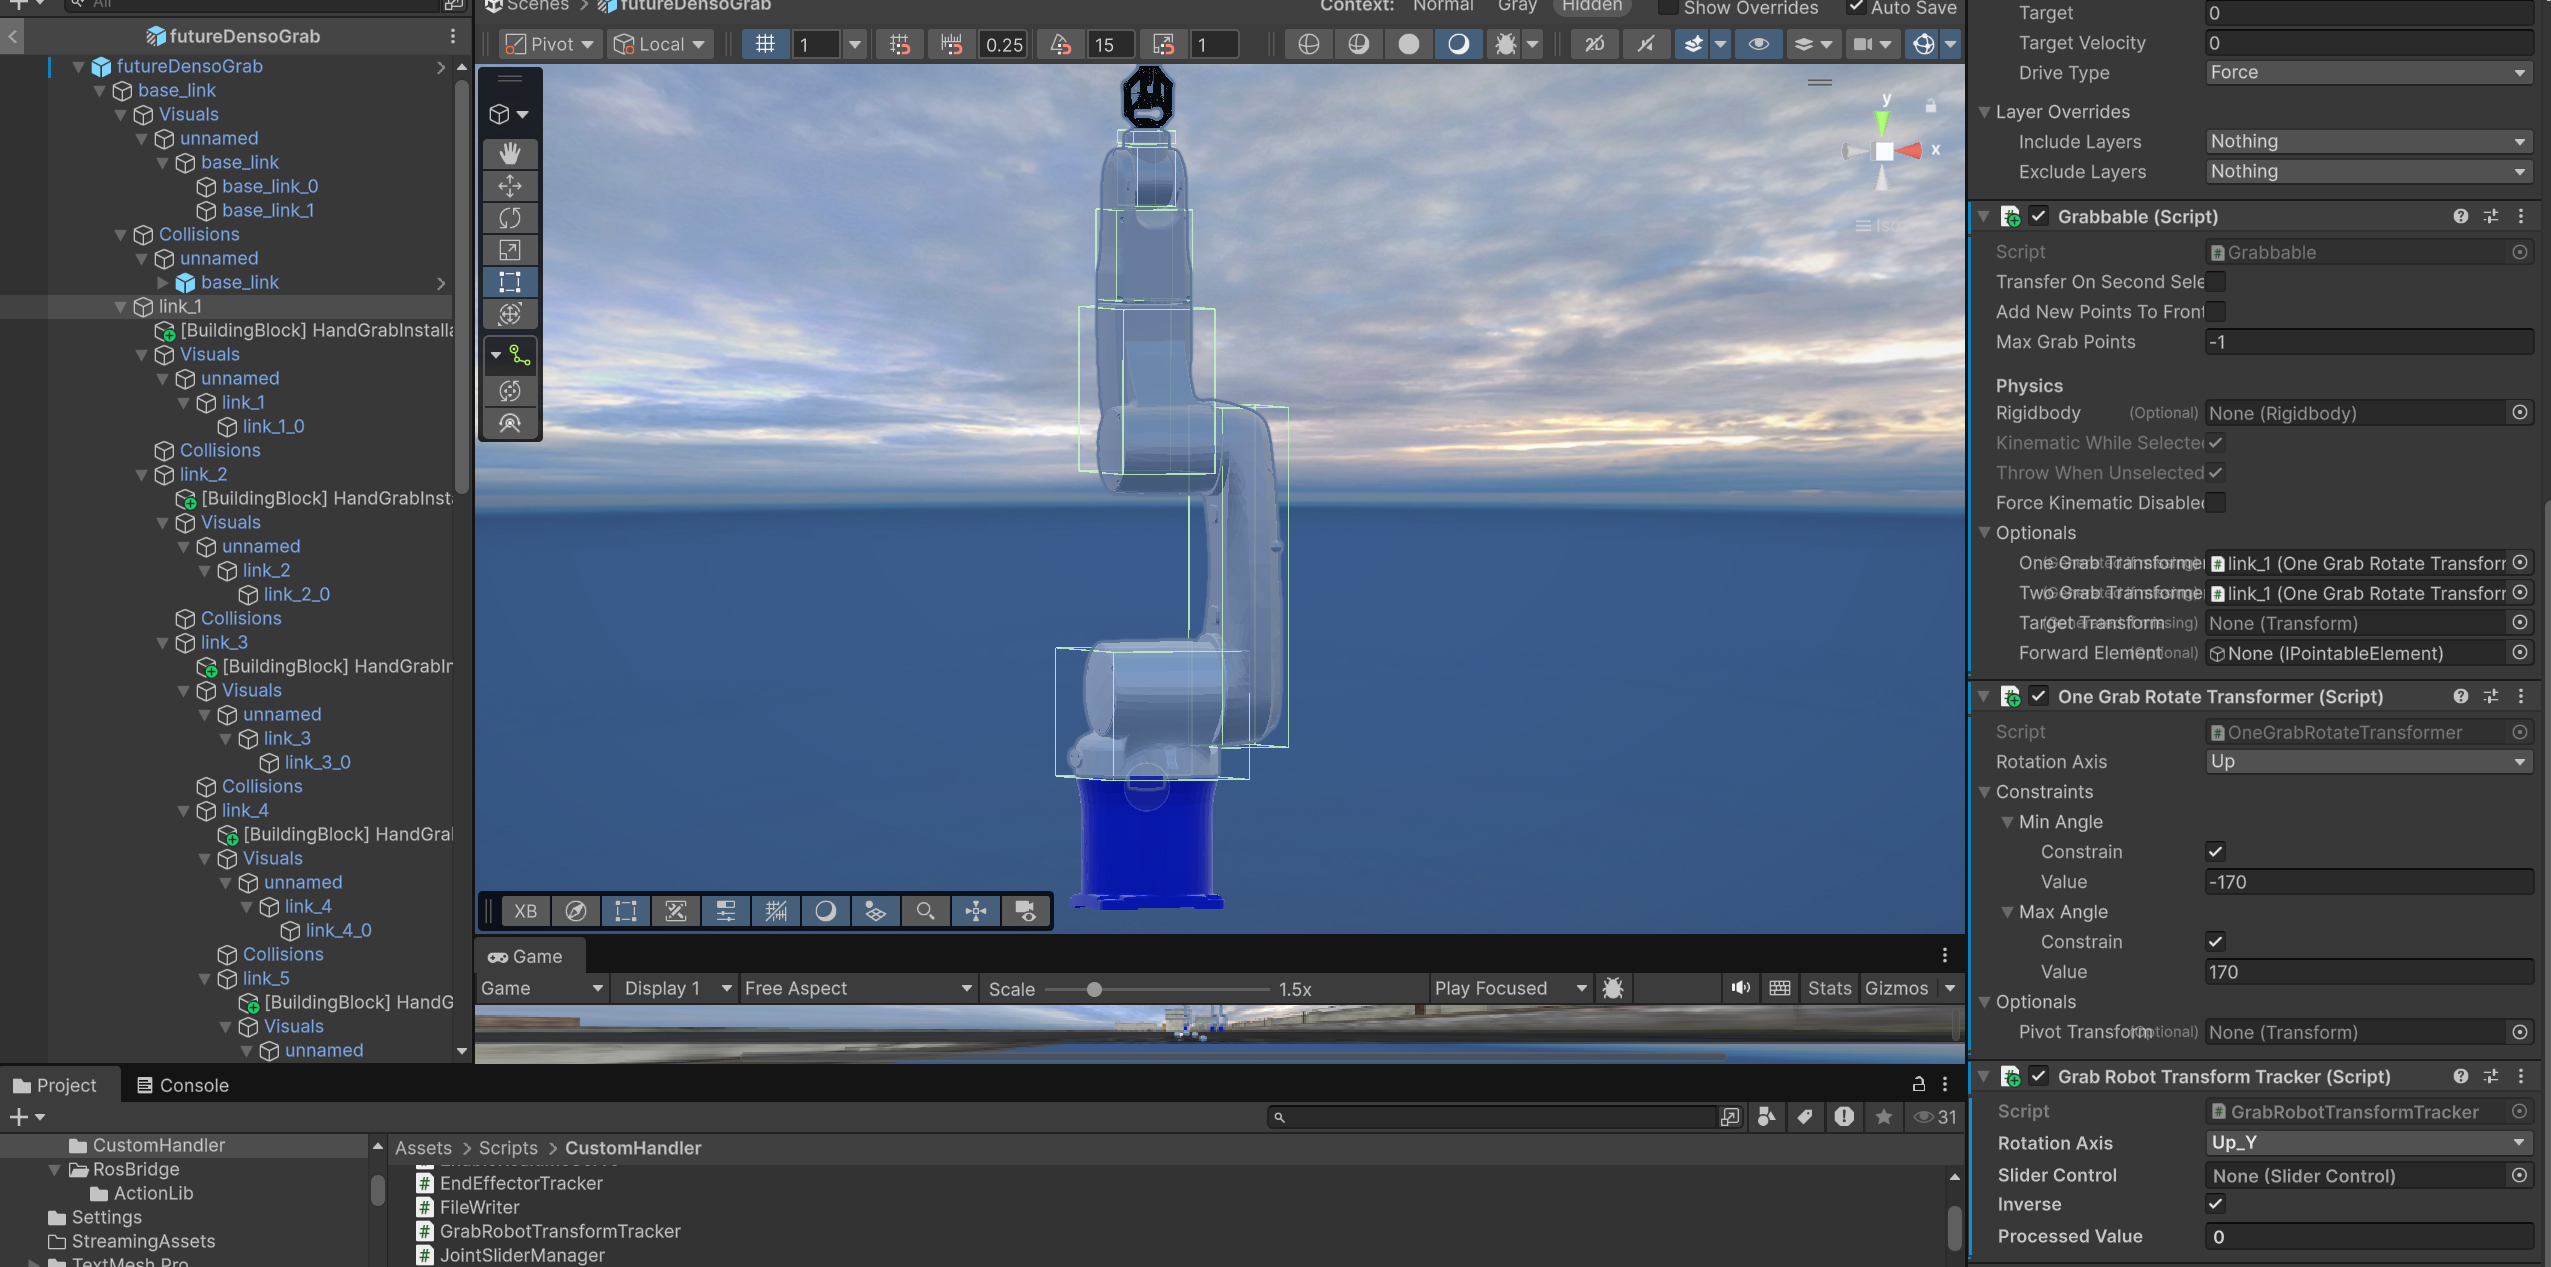
\includegraphics[width=\linewidth]{Images/Implementation/robotgrabrotate_transformer.png}
        \caption{Thiết lập OneGrabRotateTransformer}
    \end{subfigure}
    \caption{Điều khiển robot bằng tương tác nắm trực tiếp trên mô hình}
    \label{fig:robot-grab-rotate}
\end{figure}

Ở chế độ này, một mô hình 3D tương lai của robot cũng xuất hiện, cùng bộ slider mới, tuy nhiên các slider này không thể tương tác được - giá trị của nó sẽ phụ thuộc vào trạng thái của mô hình 3D "Grab Future Denso Robot". 

Về phía "Grab Future Denso Robot", ở mỗi trục sẽ được điều chỉnh để trở thành một "Grab Interactable" object, để cho phép người dùng có thể xoay từng trục bằng thao tác nắm của tay cầm hoặc bàn tay mô phỏng. OneGrabRotateTransformer được sử dụng để đảm bảo rằng khi thực hiện thao tác "grab", các trục robot chỉ có thể xoay (Rotate) quanh một trục cố định, với giới hạn min-max, tránh trường hợp người dùng cầm nắm quá tự do khiến trục bị tách rời khỏi cánh tay, hoặc trục bị xoay vượt quá ngưỡng cho phép.

Giá trị rotate của từng trục được thu thập và hiển thị lên slider để người dùng theo dõi. Khi đã xoay các trục tới vị trí mong muốn, người dùng có thể nhấn nút Execute để gửi giá trị các trục đó tới Ros2 và điều khiển cánh tay thực tế tới vị trí như yêu cầu.






\chapter{KẾT QUẢ HIỆN THỰC VÀ ĐÁNH GIÁ}

Trong chương này, nhóm sẽ trình bày kết quả của việc hiện thực hai trong 3 module chính trong kiến trúc đề xuất ban đầu cho ứng dụng điều khiển cánh tay robot bằng kính VR, bao gồm khối phần cứng (máy tính RC5 + Cánh tay robot Denso VS-6577) và phần điều khiển bằng Ros2 với PC controller.

\section{Kết quả hiện thực}

\subsection{Kết quả demo}

Video demo của hệ thống điều khiển được trình bày tại đây: \href{https://drive.google.com/drive/folders/1OyP-rfXzVsNN-aHCGCSpOcyiajlx_tWP?usp=sharing}{Demo}

\subsection{Điều khiển Robot thông qua RC5}

Ở giai đoạn hai, đề tài đã tập trung cải thiện phương thức điều khiển bằng RC5, và hiện đã có một chu trình điều khiển ổn định và đáng tin cậy hơn rất nhiều so với giai đoạn trước đó. Nhờ việc phát hiện lỗi string đơn giản với CRC length, chương trình RC5 có thể chạy liên tục trong khoảng thời gian dài mà không bị lỗi gián đoạn. Với tốc độ truyền UART được set lên 119200 bit/s, thực nghiệm trong suốt quá trình phát triển cho thấy cứ 1000 lệnh gửi xuống RC5 sẽ có 2 lần lệnh bị lỗi, và chương trình RC5 hiện tại đã giúp loại bỏ vấn đề ngưng hệ thống mỗi khi chuỗi lệnh bị hỏng.

Khi việc xử lý chuỗi được ổn định, thì luồng thực thi để di chuyển cánh tay robot cũng ổn định theo. Với việc tách các hàm chạy theo chu kì, sử dụng ring buffer để tách biệt giữa luồng xử lý chuỗi và luồng thực thi, cánh tay robot có thể chạy với tốc độ cao hơn và nhanh hơn, trong khi vẫn đảm bảo an toàn và chương trình không bị gián đoạn.

\subsection{Hệ thống điều khiển với Ros2}

Dựa trên nền tảng Ros2, đề tài đã xây dựng và tích hợp thành công nhiều module khác nhau: hiện thực Ros2-control với Hardware interface và phần driver, protocol riêng biệt, cấu hình Ros2-controllers, cấu hình MoveIt2 tích hợp với Ros2-Control, tích hợp Gazebo cho mô phỏng thay thế Hardware Interface, sử dụng MoveIt-Servo, tạo custom Service Provider và Action Server, tích hợp RosBridge server cho giao tiếp Ros thông qua web socket. Hiện tại, dự án đang có đến 10 Ros-packages được sử dụng. Chi tiết về cách cài đặt có thể xem qua ở phần Readme của Repo: \href{https://github.com/ngoccatt/ros2_arctos_HCMUT/tree/cat_impl}{ros2\_arctos\_HCMUT}.

Sau khi đã clone repo và chuẩn bị hết tất cả những phụ thuộc môi trường (package ros-humble, python...), ta build dự án từ thư mục gốc bằng lệnh:

\begin{lstlisting}[style=bashstyle]
colcon build --symlink-install
\end{lstlisting}

Quá trình build sẽ diễn ra trong vài phút, và thực hiện build 10 module khác nhau như kết quả dưới:

\begin{lstlisting}[style=bashstyle]
colcon build --symlink-install
Starting >>> serial
Starting >>> denso_description
Starting >>> denso_interfaces
Starting >>> denso_moveit_servo
Starting >>> file_server2
Finished <<< denso_description [0.31s]
Starting >>> denso_moveit_config
Finished <<< serial [0.42s]
Starting >>> denso_motor_driver
Finished <<< denso_moveit_servo [0.42s]
Finished <<< denso_moveit_config [0.33s]
Finished <<< denso_motor_driver [0.39s]
Starting >>> denso_hardware_interface
Finished <<< file_server2 [1.37s]
Finished <<< denso_interfaces [1.41s]
Starting >>> denso_remote_control
Finished <<< denso_hardware_interface [0.83s]
Starting >>> denso_bringup
Finished <<< denso_remote_control [0.77s]
Finished <<< denso_bringup [1.64s]

Summary: 10 packages finished [4.25s]
\end{lstlisting}

Sau khi build thành công, ta "source" dự án để Ros2 biết được sự tồn tại của chương trình:

\begin{lstlisting}[style=bashstyle]
source install/setup.bash
\end{lstlisting}

Sau đó, ta có thể lần lượt chạy các module chính của dự án.

\subsubsection{Hệ thống điều khiển chính với Ros2-Control và MoveIt}

Để chạy chương trình điều khiển chính, người dùng gõ lệnh sau vào terminal

\begin{lstlisting}[style=bashstyle]
ros2 launch denso_bringup denso_bringup.launch.py use_sim_time:=false
\end{lstlisting}

File bringup có nhiệm vụ chạy hết tất cả các module liên quan, bao gồm:

\begin{itemize}
    \item Ros2-control manager
    \item Robot state publisher
    \item JointStateBoardcaster Ros2 Controller
    \item Denso\_arm\_controller
    \item Denso\_hand\_controller
    \item Rviz2
    \item MoveIt2 (MoveGroup)
    \item V4L2 camera node 1
    \item V4L2 camera node 2
\end{itemize}

Toàn bộ module Ros2-Control kèm controllers đều được khởi chạy, có sự tích hợp bởi MoveIt2 phía trên cho planning và Execution. Ngoài ra, các camera node cũng được khởi chạy để plublish các topic camera mà ứng dụng VR có thể sử dụng.

\textbf{Giao diện điều khiển cánh tay robot VS-6577 với Rviz}

Khởi chạy thành công, giao diện Rviz sẽ hiển thị ra như hình, bao gồm mô hình 3D của cánh tay và cả phần tay gắp. Lưu ý rằng mô hình tay gắp trong Rviz hiện tại không phản ánh chính xác hoạt động của của tay gắp, mà được đơn giản hóa hơn. Lý do là vì tay gắp thực tế có liên kết trục phức tạp và không thể xây dựng quan hệ một cha - một con trong URDF.

Trong Rviz, ta có thể thay đổi planning group để thay đổi đối tượng cần điều khiển. \textbf{denso\_arm} dùng để điều khiển sáu trục của cánh tay, còn \textbf{denso\_hand} dùng để điều khiển phần tay gắp. Velocity Scaling và Accel Scaling là tỉ lệ của vận tốc và gia tốc tối đa được cấu hình cho cánh tay. Hiện tại, đồ án nhận thấy Velocity scaling 0.4 cùng Accel. Scaling 0.3 đem lại hiệu quả điều khiển ổn định và mượt mà nhất.

\begin{figure}[H]
    \centering
    \begin{subfigure}{0.48\linewidth}
        \centering
        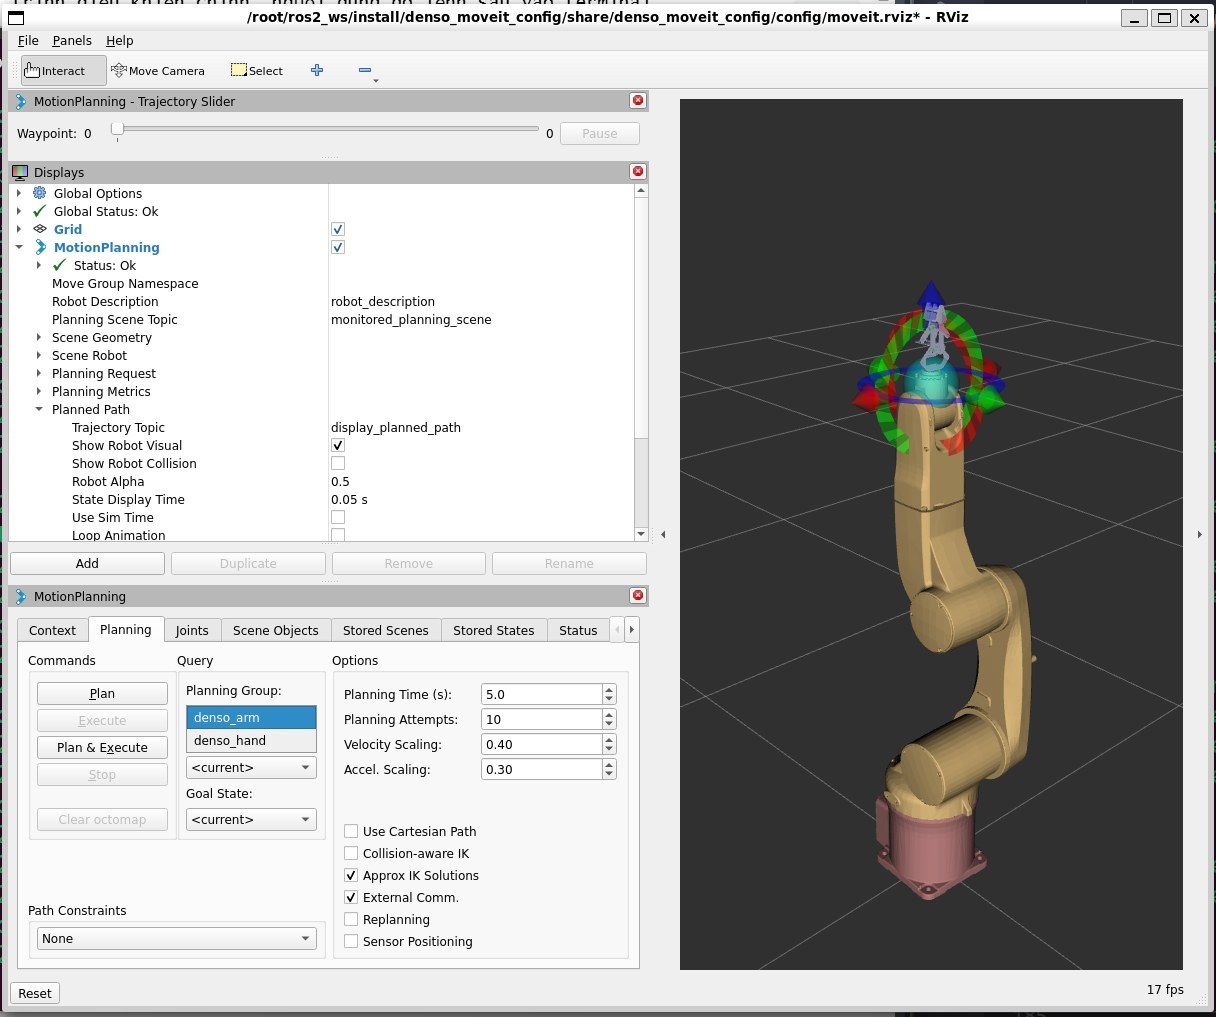
\includegraphics[width=\linewidth]{Images/Implementation/bringup1.jpg}
        \caption{Giao diện điều khiển chính với Rviz}
    \end{subfigure}
    \hfill
    \begin{subfigure}{0.48\linewidth}
        \centering
        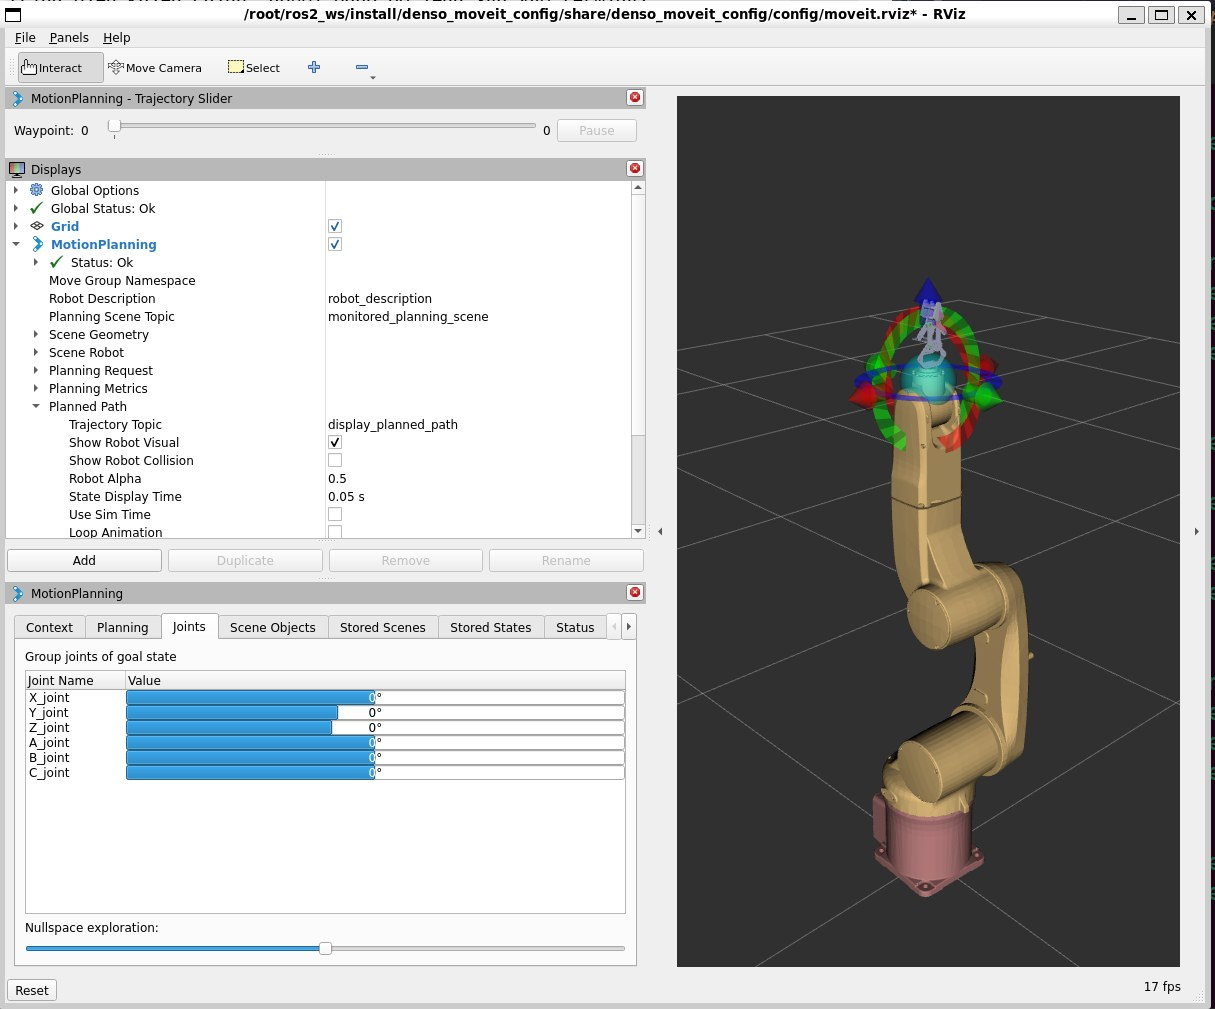
\includegraphics[width=\linewidth]{Images/Implementation/bringup2.jpg}
        \caption{Điều khiển các trục phần cánh tay}
    \end{subfigure}
    \hfill
    \begin{subfigure}{0.48\linewidth}
        \centering
        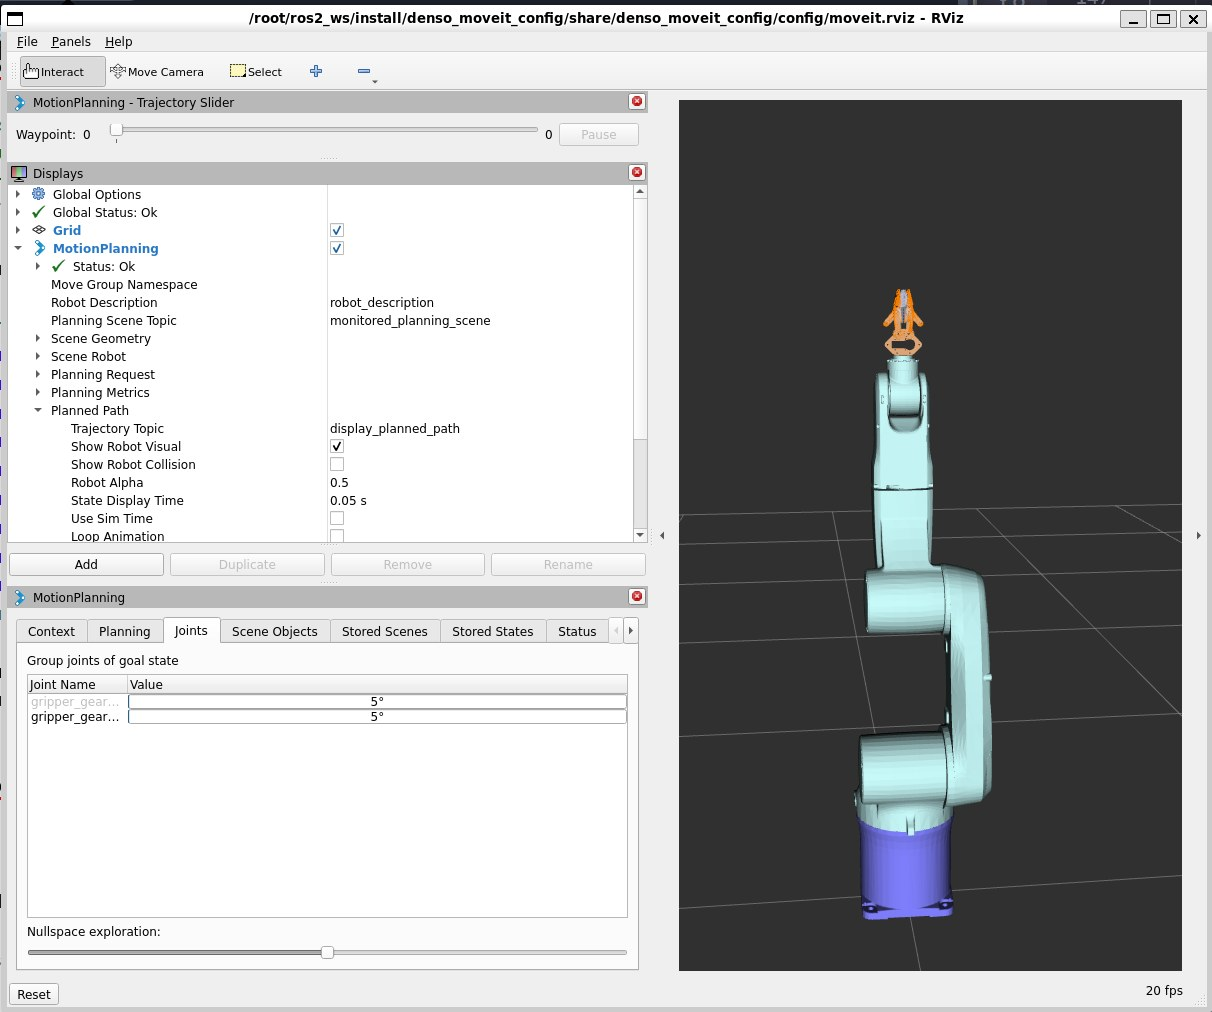
\includegraphics[width=\linewidth]{Images/Implementation/bringup3.jpg}
        \caption{Điều khiển các trục phần tay gắp}
    \end{subfigure}
    \caption{Kết quả khởi chạy hệ thống mô phỏng với Gazebo}
    \label{fig:eval-gazebo-bringup}
\end{figure}

Trong hộp thoại MotionPlanning, ở thẻ Joint, ta có thể tùy ý xoay từng trục cánh tay đích (goal state) để xem trạng thái của chúng. Các giá trị góc xoay sẽ được giới hạn, tuân theo thông tin được cấu hình ở file URDF hoặc các file cấu hình khác, nếu có. Khi cần điều khiển robot tương ứng, ta có thể chuyển qua tab Planning. Ở đây có hai chức năng: khi nhấn \textbf{Plan}, MoveIt sẽ thực hiện việc tính toán dựa theo thông tin về robot cũng như thuật toán động lực học đã chọn, và để xuất ra đường đi, hay quỹ đạo tối ưu để đưa robot từ vị trí hiện tại sang vị trí Goal. Lựa chọn \textbf{Execute} sẽ chỉ sáng lên sau khi planning hoàn tất, tức thực thi quá trình điều khiển để cánh tay thực tế có thể đi tới vị trí mục tiêu. Lựa chọn \textbf{Plan \& Execute} sẽ thực hiện tuần tự \textbf{Plan} và tự động \textbf{Execute} sau khi \textbf{Plan} hoàn tất.

Khi bấm \textbf{Execute}, Moveit sẽ bắt đầu gửi các trajectory tới Controller của cánh tay robot, và yêu cầu cánh tay robot quay dần để đạt tới vị trí đích. Từng giá trị Trajectory được truyền xuống Controller, tham gia vai trò của \textbf{update} trong chu kì ba bước. Sau \textbf{update}, các \lstinline[style=inlinecode]{command_interface} sẽ được ghi vào giá trị điều khiển, và \textbf{write} sử dụng các \lstinline[style=inlinecode]{command_interface}, tổng hợp thành một lệnh điều khiển đưa xuống máy RC5 theo định dạng phù hợp. Tiếp đó, \textbf{read} đọc trạng thái góc quay thực tế của cánh tay phản hồi từ RC5, cập nhật vào các \lstinline[style=inlinecode]{state_interface}. Giá trị trạng thái cũng được phản ánh ngay trên mô hình cánh tay Robot trên Rviz, và người dùng có thể thấy mô hình 3D mờ dần dần di chuyển tới vị trí đích.

\subsubsection{Hệ thống điều khiển mô phỏng với Ros2-Control, MoveIt2 và Gazebo}

Gazebo được tích hợp vào hệ thống để giúp cho việc phát triển ứng dụng nhanh chóng hơn, an toàn hơn nhờ môi trường mô phỏng, trước khi thử nghiệm trên cánh tay thực tế. Để chạy hệ thống điều khiển với Gazebo, chạy lện sau trong cửa sổ terminal:

\begin{lstlisting}[style=bashstyle]
ros2 launch denso_bringup gz_denso_bringup.launch.py use_sim_time:=true
\end{lstlisting}

So với file bringup cho thiết bị thực tế, gz\_denso\_bringup sẽ chạy các tác vụ sau:

\begin{itemize}
    \item Gazebo Sim (Ignition)
    \item Sinh mô hình robot trong Gazebo
    \item Cầu nối (bridge) giữa clock của Ros2 và clock của Gazebo
    \item JointStateBoardcaster Ros2 Controller
    \item Denso\_arm\_controller
    \item Denso\_hand\_controller
    \item Rviz2
    \item MoveIt2 (MoveGroup)
    \item V4L2 camera node 1
    \item V4L2 camera node 2
\end{itemize}

Ngoài việc chạy thêm các tác vụ liên quan tới Gazebo, lưu ý rằng Ros2-control manager đã không khởi chạy. Lý do là Gazebo khi được chọn là Hardware Interface thay thế (sử dụng gz\_ros2\_control::GazeboSimROS2ControlPlugin), nó sẽ tự chạy controller manager tự động, nên việc khởi chạy ros2-controol manager ở bringup là không cần thiết.

\begin{figure}[H]
    \centering
    \begin{subfigure}{0.48\linewidth}
        \centering
        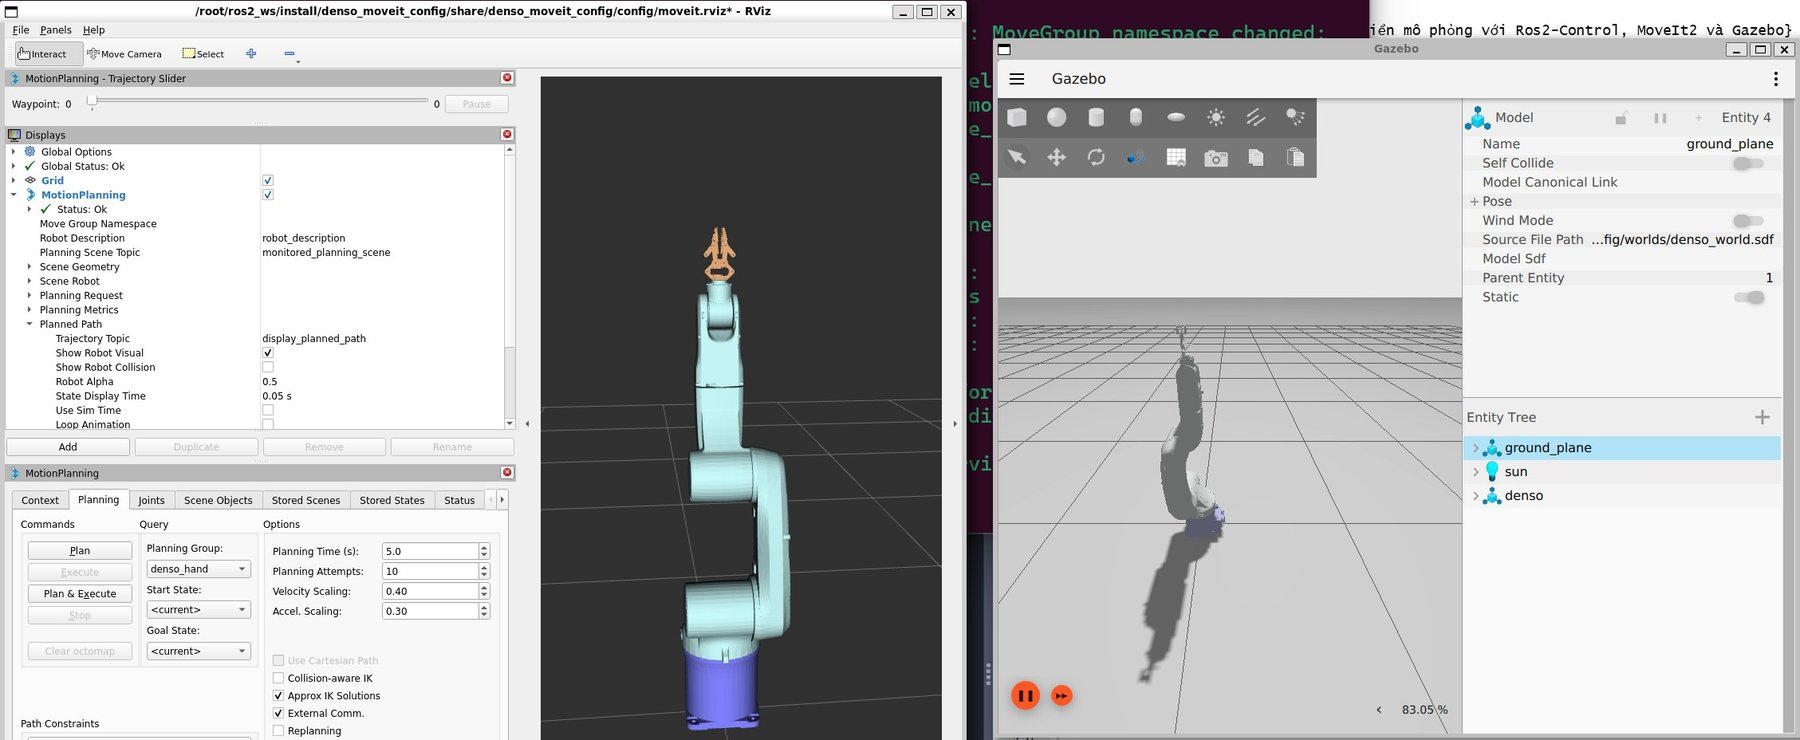
\includegraphics[width=\linewidth]{Images/Implementation/gz_bringup_1.jpg}
        \caption{Gazebo mô phỏng cánh tay robot}
    \end{subfigure}
    \hfill
    \begin{subfigure}{0.48\linewidth}
        \centering
        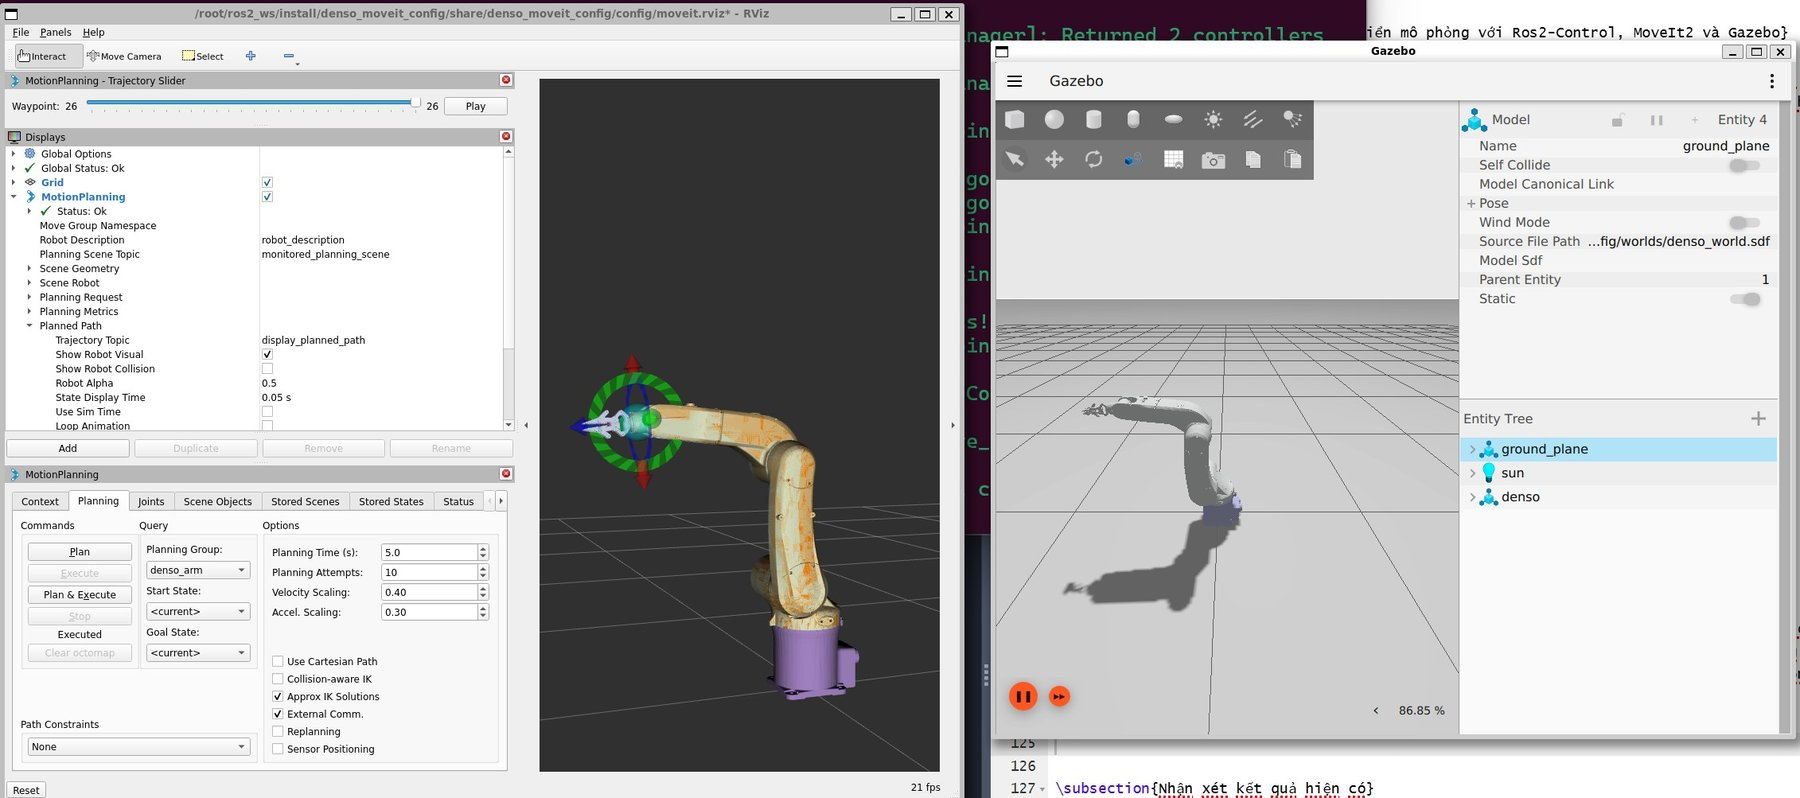
\includegraphics[width=\linewidth]{Images/Implementation/gz_bringup_2.jpg}
        \caption{Rviz đồng bộ với mô phỏng Gazebo}
    \end{subfigure}
    \caption{Kết quả khởi chạy hệ thống mô phỏng với Gazebo}
    \label{fig:eval-gazebo-bringup}
\end{figure}

Với hệ thống mô phỏng này, ta hoàn toàn có thể dùng Rviz để Planning, Execute các trục robot và điều khiển tay gắp mà không cần thiết bị thật, đồng thời thấy được phản hồi thay đổi trạng thái cánh tay khi Gazebo thực hiện thao tác di chuyển. Thêm nữa, ta sẽ không thể thực hiện kiểm thử module Hardware Interface do Gazebo đã thay thế module này trong vai trò thực hiện lệnh điều khiển và cập nhật trạng thái. Hệ thống mô phỏng sẽ chỉ hữu ích trong việc kiểm tra các tính năng từ tầng Hardware Interface trở lên: Các Controller, MoveIt và ứng dụng dựa trên MoveIt.

\subsubsection{Denso MoveIt-Servo Service provider}

Sau khi đã khởi chạy hệ thống chính, các module ứng dụng có thể lần lượt chạy để cung cấp phương thức điều khiển từ bên ngoài. Gõ lệnh sau vào terminal để chạy Denso Moveit-Servo:

\begin{lstlisting}[style=bashstyle]
ros2 launch denso_moveit_servo denso_moveit_servo.launch.py
\end{lstlisting}

Để có thể kiểm thử nhanh tính năng điều khiển với MoveIt Servo, ta có thể chạy thêm chương trình sau ở một terminal khác để xoay các trục robot bằng bàn phím:

\begin{lstlisting}[style=bashstyle]
ros2 run denso_moveit_servo servo_keyboard_input
\end{lstlisting}

\begin{figure}[H]
    \centering
    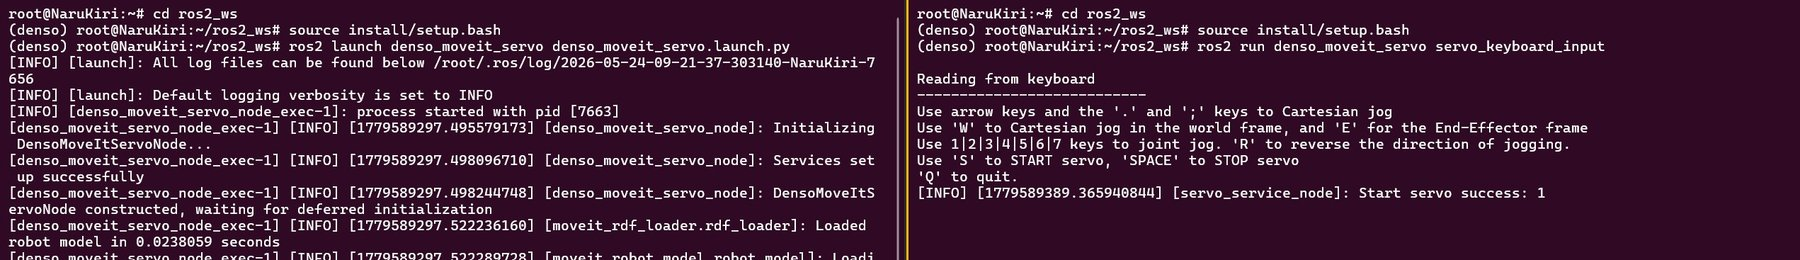
\includegraphics[width=0.9\linewidth]{Images/Implementation/denso_moveitservo.jpg}
    \caption{Node Denso MoveIt-Servo sau khi khởi chạy}
    \label{fig:eval-moveit-servo-node}
\end{figure}

\subsubsection{Denso Remote Control Action Server}

Tiếp theo, ta có thể chạy Action Server để nhận lệnh điều khiển Action dạng MoveToPose, để xoay robot tới vị trí yêu cầu. Ở một terminal khác, chạy lệnh sau:

\begin{lstlisting}[style=bashstyle]
ros2 launch denso_remote_control remote_control.launch.py
\end{lstlisting}

Ta có thể kiểm thử Action server này bằng việc gửi một Action Goal, với định dạng lệnh như sau (lưu ý phải source vào workspace trước khi sử dụng)

\begin{lstlisting}[style=bashstyle]
ros2 action send_goal /move_to_pose denso_interfaces/action/MoveToPose "{pose: {position: {x: 0.0, y: 0.0, z: 0.0}, orientation: {x: 0.0, y: 0.0, z: 0.0, w: 1.0}}, joints: [0.0, -0.5, 1.0, 0.0, 0.5, 0.0], use_pose: false}"
\end{lstlisting}

\begin{figure}[H]
    \centering
    \begin{subfigure}{0.48\linewidth}
        \centering
        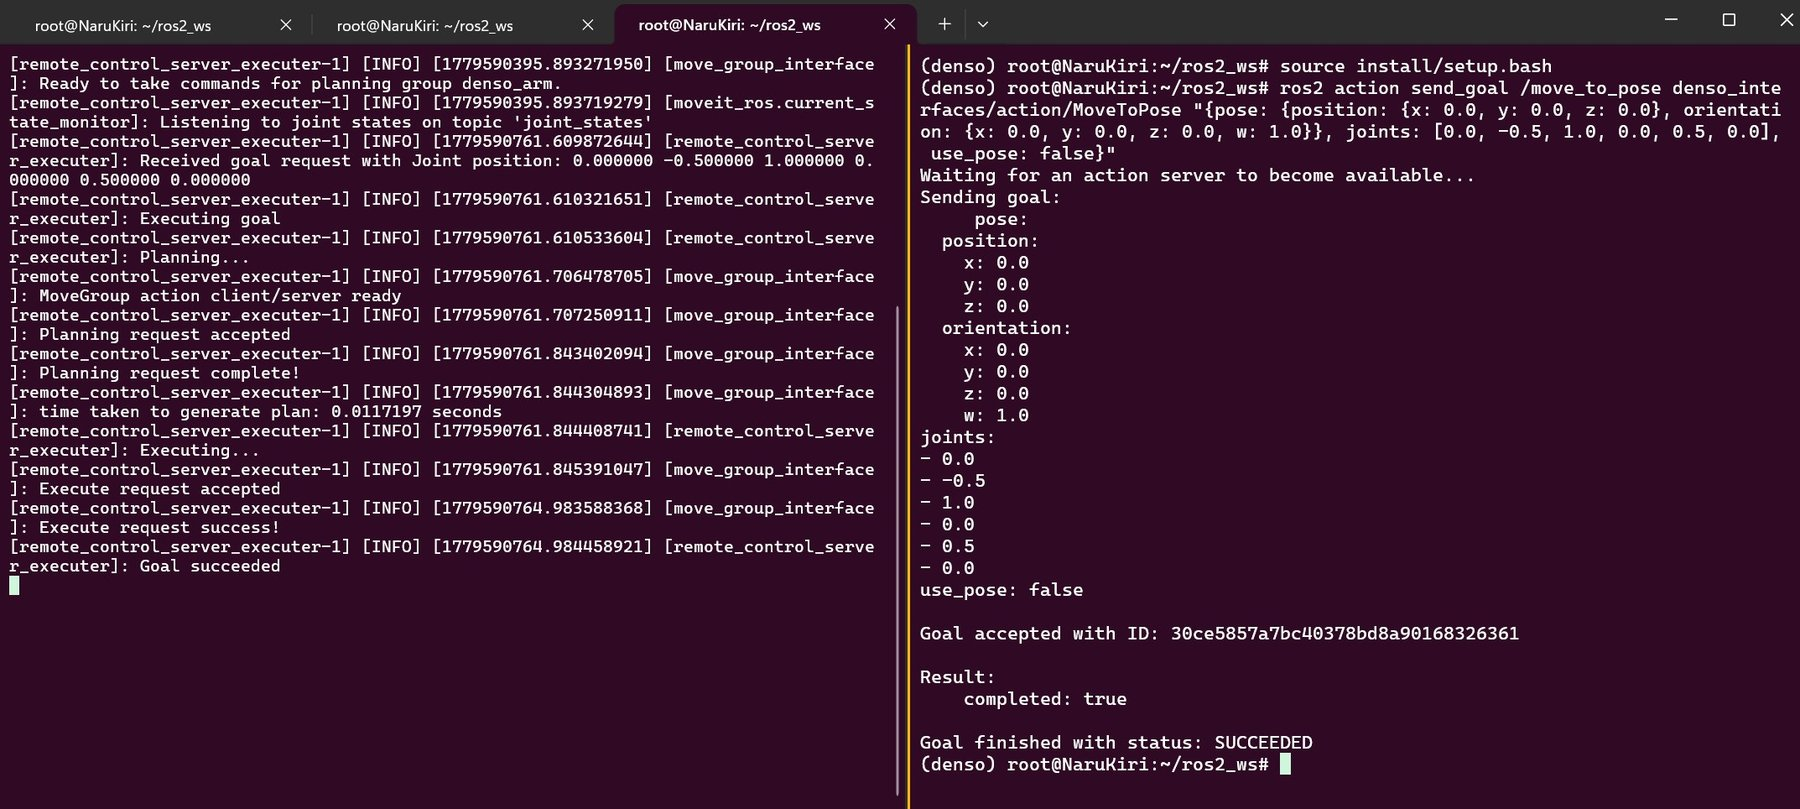
\includegraphics[width=\linewidth]{Images/Implementation/remote_control.jpg}
        \caption{Action Server Remote Control}
    \end{subfigure}
    \hfill
    \begin{subfigure}{0.48\linewidth}
        \centering
        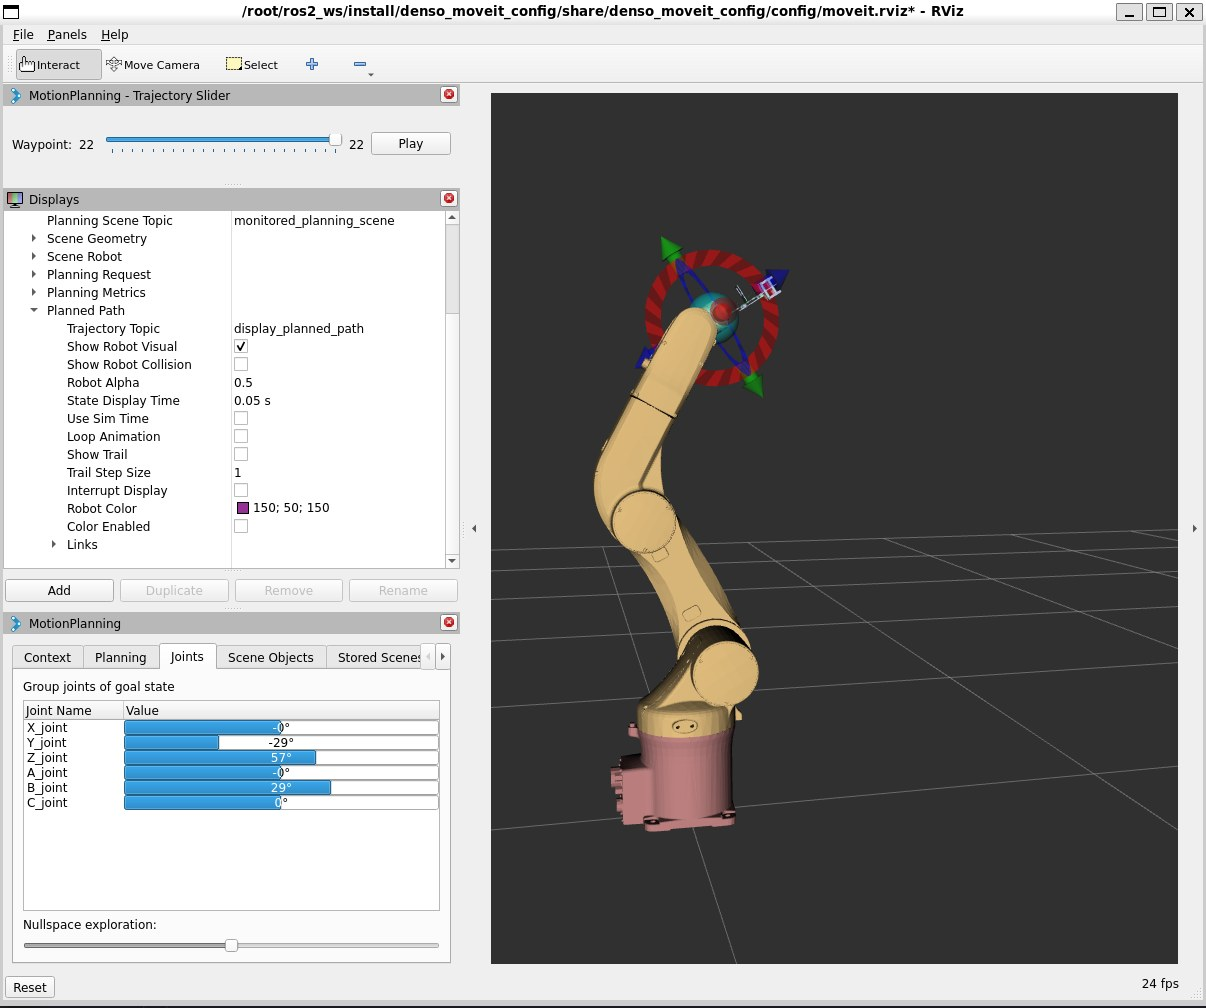
\includegraphics[width=\linewidth]{Images/Implementation/remote_control_1.jpg}
        \caption{Luồng phản hồi của Action Server}
    \end{subfigure}
    \caption{Kết quả kiểm thử Denso Remote Control}
    \label{fig:eval-remote-control}
\end{figure}

Lệnh trên thực hiện việc điều khiển robot bằng cách sử dụng danh sách giá trị các trục (theo đơn vị rad). Mô phỏng với Gazebo cho thấy robot đã xoay tới vị trí mong muốn.

\subsubsection{RosBridge Server}

Để có thể cho ứng dụng VR giao tiếp với Ros thông qua Web socket, ta cần chạy thêm RosBridge Server. Lệnh sau được sử dụng để chạy server cho kết nối:

\begin{lstlisting}[style=bashstyle]
ros2 launch file_server2 ros_sharp_communication.launch.py
\end{lstlisting}

\begin{figure}[H]
    \centering
    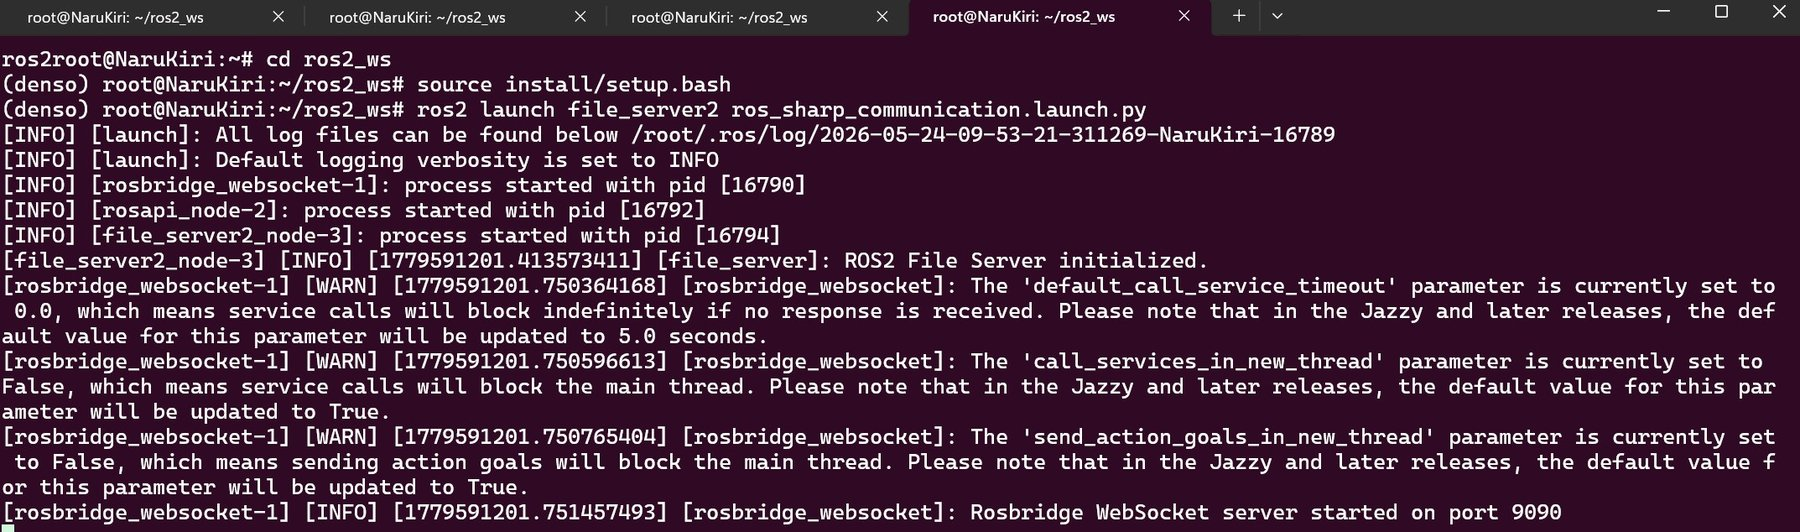
\includegraphics[width=0.90\linewidth]{Images/Implementation/rosbridge_server.jpg}
    \caption{RosBridge Server sẵn sàng kết nối cho ứng dụng VR}
    \label{fig:eval-rosbridge-server}
\end{figure}

RosBridge server được khởi chạy tại port 9090, cho phép ứng dụng Unity với Ros-Sharp có thể kết nối tới và sử dụng các topic/service/action tự do.

\subsubsection{Đánh giá về độ trễ Execution trên thiết bị thực tế}

Trong quá trình phát triển, đề tài nhận thấy rằng việc điều khiển cánh tay thực tế luôn có độ trễ: cánh tay robot cần xoay các motor để di chuyển, cần phải có quá trình gia tốc, giảm tốc, có ma sát và ảnh hưởng bởi trọng lực, nên giả định lý tưởng: "với một lệnh điều khiển, cánh tay robot sẽ xoay hoàn tất trước khi nhận lệnh tiếp theo" là khó để đạt được, ít nhất là với hệ thống hiện tại, khi Ros2-Control tính toán trước chuỗi trajectory và gửi lần lượt chuỗi đó theo chu kì cố định. Chính vì vậy, đề tài đã thực hiện nhiều lần kiểm thử để tìm một cấu hình tối ưu, nhằm đồng bộ nhất có thể giữa tần số điều khiển của Ros2 và thời gian hoạt động của cánh tay robot, gồm:

\begin{itemize}
    \item Cấu hình tốc độ tối đa của từng trục theo tài liệu kĩ thuật chính thức của cánh tay
    \item Sử dụng Velocity scaling và acceleration scaling gần tương đồng (nhỏ hơn) so với tốc độ của cánh tay ở RC5. Ví dụ, Velocity scaling là 0.4 thì tốc độ cánh tay sẽ là 46\%
    \item Lựa chọn tần số 10Hz cho hoạt động điều khiển của Ros2-Control, qua đó cho phép  hoạt động từ phía RC5 diễn ra trong 100ms với ba giai đoạn: Nhận lệnh UART (~10ms), Xử lý lệnh UART dạng chuỗi (20-30ms), Xoay cánh tay (60-70ms).
    \item Phản hồi trạng thái cánh tay từ RC5 lên Ros2 diễn ra mỗi 100ms, tương tự với chu kì điều khiển Ros2
\end{itemize}

"Độ trễ" được tính toán dựa trên mỗi lần planning với MoveIt2, là sai lệch kể từ lúc Ros2-control ngưng gửi lệnh xuống RC5 cho tới khi cánh tay robot hoàn thành hành động xoay. Bảng thống kê độ trễ từ hai phiên kiểm thử thực tế với tổng cộng 25 goals được trình bày dưới đây:

\begin{figure}[H]
\centering
\begin{tikzpicture}
\begin{axis}[
    width=0.92\linewidth,
    height=6.5cm,
    xlabel={Goal},
    ylabel={Thời gian (ms)},
    xmin=0.5, xmax=25.5,
    ymin=0, ymax=15000,
    xtick={1,2,...,25},
    xticklabel style={font=\scriptsize},
    yticklabel style={font=\small},
    ytick={0,2000,4000,6000,8000,10000,12000,14000},
    grid=both,
    grid style={line width=0.3pt, draw=gray!30},
    major grid style={line width=0.5pt, draw=gray!50},
    legend style={at={(0.98,0.98)}, anchor=north east, font=\small,
                  draw=gray!50, fill=white, row sep=1pt},
    legend cell align=left,
    tick align=outside,
    axis lines=left,
    scaled ticks=false,
]
% T_tong
\addplot[color=blue!70, mark=square*, mark size=2pt, line width=1.2pt]
coordinates {
    (1,5797)(2,7898)(3,3396)(4,5698)
    (5,6698)(6,7698)(7,6296)(8,3699)(9,13798)(10,5699)
    (11,5799)(12,6198)(13,9399)(14,4799)(15,6898)(16,4898)
    (17,1699)(18,3199)(19,1599)(20,1299)(21,2199)
    (22,5698)(23,7098)(24,4399)(25,9499)
};
\addlegendentry{$T_\text{tổng}$}
% T_gui
\addplot[color=teal, mark=triangle*, mark size=2.5pt, line width=1.2pt, dashed]
coordinates {
    (1,3698)(2,6598)(3,1497)(4,3700)
    (5,3699)(6,5799)(7,5797)(8,1599)(9,10199)(10,3099)
    (11,3099)(12,4399)(13,5799)(14,3099)(15,5098)(16,2498)
    (17,899)(18,1099)(19,899)(20,599)(21,600)
    (22,2999)(23,5299)(24,1999)(25,5899)
};
\addlegendentry{$T_\text{gửi}$}
% T_dung
\addplot[color=red!80, mark=*, mark size=2.5pt, line width=1.5pt]
coordinates {
    (1,2099)(2,1300)(3,1899)(4,1999)
    (5,2999)(6,1899)(7,499)(8,2100)(9,3600)(10,2599)
    (11,2700)(12,1800)(13,3600)(14,1699)(15,1800)(16,2399)
    (17,800)(18,2099)(19,700)(20,700)(21,1599)
    (22,2699)(23,1800)(24,2400)(25,3599)
};
\addlegendentry{$T_\text{dừng}$ (độ trễ vật lý)}
% Duong trung binh T_dung
\addplot[color=red!80, line width=0.8pt, dotted, domain=0.5:25.5] {2055};
\addlegendentry{$\overline{T_\text{dừng}}$ = 2055\,ms}
\end{axis}
\end{tikzpicture}
\caption{Biểu đồ độ trễ Execution theo từng goal -- đường đỏ ($T_\text{dừng}$) là độ trễ vật lý sau khi Ros2 ngừng gửi lệnh}
\label{fig:moveit-latency-chart}
\end{figure}

\begin{table}[H]
\centering
\caption{Thống kê tổng hợp độ trễ Execution của MoveIt2 ($N = 25$ goals)}
\label{tab:moveit-execution-latency}
\begin{tblr}{
    colspec = {|X[3.5,l]|X[1.2,c]|X[1.2,c]|X[1.4,c]|X[1.2,c]|},
    hlines,
    row{1} = {font=\bfseries, bg=gray!20},
}
Chỉ số & Min (ms) & TB (ms) & Trung vị (ms) & Max (ms) \\
$T_\text{gửi}$ (\texttt{goal\_to\_last\_write}) & 599 & 3599 & 3099 & 10199 \\
$T_\text{dừng}$ (\texttt{last\_write\_to\_settle}) & 499 & 2055 & 1999 & 3600 \\
$T_\text{tổng}$ (\texttt{goal\_to\_settle}) & 1299 & 5654 & 5699 & 13798 \\
\end{tblr}
\end{table}

Tiêu chí đánh giá trọng tâm là $T_\text{dừng}$ -- khoảng thời gian sau khi MoveIt2 ngừng gửi lệnh mà cánh tay vẫn tiếp tục di chuyển do quán tính cơ học. Đây là giai đoạn Ros2 không còn can thiệp nhưng robot chưa dừng hẳn, thể hiện trực tiếp độ lệch giữa trạng thái điều khiển phần mềm và trạng thái vật lý của cánh tay.

$T_\text{dừng}$ đo được trung bình \textbf{2055\,ms} (trung vị 1999\,ms), dao động từ 499\,ms đến 3600\,ms. Đáng chú ý là $T_\text{dừng}$ ít phụ thuộc vào độ dài quỹ đạo hơn $T_\text{gửi}$: ngay cả với các chuyển động nhỏ (goals 17, 19, 20 -- $T_\text{gửi}$ chỉ 599–899\,ms), $T_\text{dừng}$ vẫn đạt 700–800\,ms, phản ánh thời gian giảm tốc tối thiểu cần thiết để cơ cấu dừng hoàn toàn. Với chuyển động lớn hơn, $T_\text{dừng}$ tăng lên 2000–3600\,ms do động năng cơ học tích lũy lớn hơn.

$T_\text{gửi}$ trung bình \textbf{3599\,ms} ($\approx$\,64\% tổng thời gian) tương đương khoảng 36 bước waypoints tại 10\,Hz. Giá trị này phụ thuộc trực tiếp vào độ phức tạp của quỹ đạo: goal~9 (ngoại lệ, nền vàng) có $T_\text{gửi}$ = 10199\,ms ($\approx$\,102 waypoints) do nhiều bậc tự do đồng thời di chuyển góc lớn, dẫn đến $T_\text{tổng}$ = 13798\,ms.

Nhìn chung, $T_\text{tổng}$ trung bình \textbf{5654\,ms} (trung vị 5699\,ms) là tổng hợp của cả hai giai đoạn. Với cấu hình Velocity scaling 0.4 -- Accel. scaling 0.3 và chu kỳ điều khiển 100\,ms, $T_\text{dừng}$ $\approx$\,2\,s là mức độ trễ vật lý cần chấp nhận trong ứng dụng điều khiển từ kính VR: sau khi thao tác, người dùng cần chờ khoảng 2\,s để cánh tay dừng hoàn toàn và sẵn sàng nhận lệnh tiếp theo.

\subsection{Ứng dụng VR điều khiển cánh tay robot}

Ứng dụng VR được xây dựng thành công và hầu như không có bất kì xung đột package nào - ứng dụng có thể được build thành một file cài đặt và chạy độc lập trên kính VR Meta Quest 3. Các tính năng của ứng dụng cho phép người dùng tự do lựa chọn phương thức điều khiển cánh tay robot và việc điều khiển có tính ổn định, đồng bộ cao với cánh tay thực tế thông qua giao tiếp Ros-sharp. 

\subsubsection{Các tính năng của ứng dụng}

Các tính năng được hỗ trợ bởi ứng dụng bao gồm:

\textbf{Kết nối/ Ngắt kết nối với Ros2 sử dụng địa chỉ IP và port}

\begin{figure}[H]
    \centering
    \begin{subfigure}{0.48\linewidth}
        \centering
        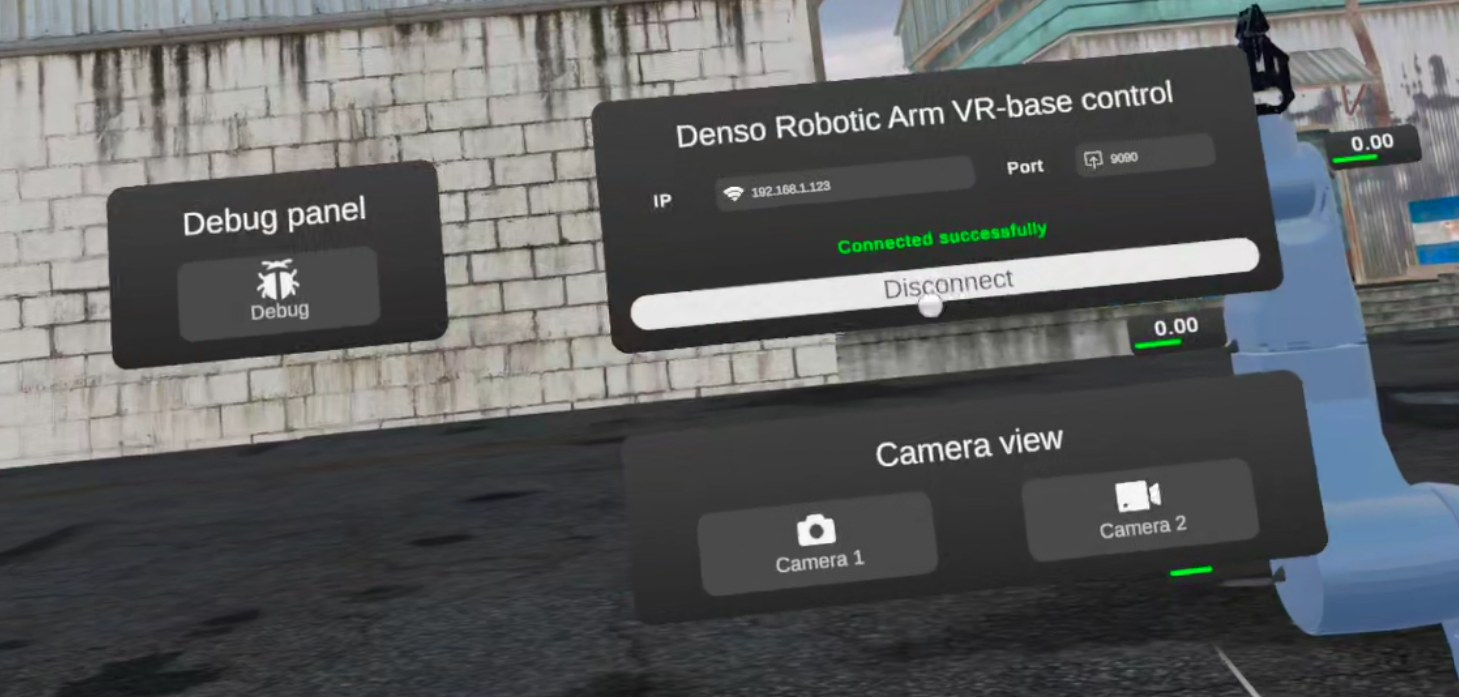
\includegraphics[width=\linewidth]{Images/Implementation/vr_connect.jpg}
        \caption{Trạng thái đã kết nối}
    \end{subfigure}
    \hfill
    \begin{subfigure}{0.48\linewidth}
        \centering
        
\includegraphics[width=\linewidth]{Images/Implementation/vr_disconnect.jpg}
        \caption{Trạng thái ngắt kết nối}
    \end{subfigure}
    \caption{Giao diện kết nối Ros2 trong ứng dụng VR}
    \label{fig:eval-vr-connect-disconnect}
\end{figure}

Khi kết nối thành công, các module và bảng điều khiển khác sẽ hiện ra để người dùng điều khiển robot. Thêm nữa, mọi bảng điều khiển trong ứng dụng để có thể tương tác và nắm được, nên người dùng cũng có thể tự do sắp xếp các bảng điều khiển trong môi trường cho tiện sử dụng.

\textbf{Bật/Tắt hai camera môi trường để quan sát}

Sau khi kết nối, người dùng có thể nhấn vào nút Camera 1 / Camera 2 để mở màn hình video xem dữ liệu truyền từ camera thông qua Ros2 topic. Debug panell được cung cấp kèm theo cho mục đích debug.

\begin{figure}[H]
    \centering
    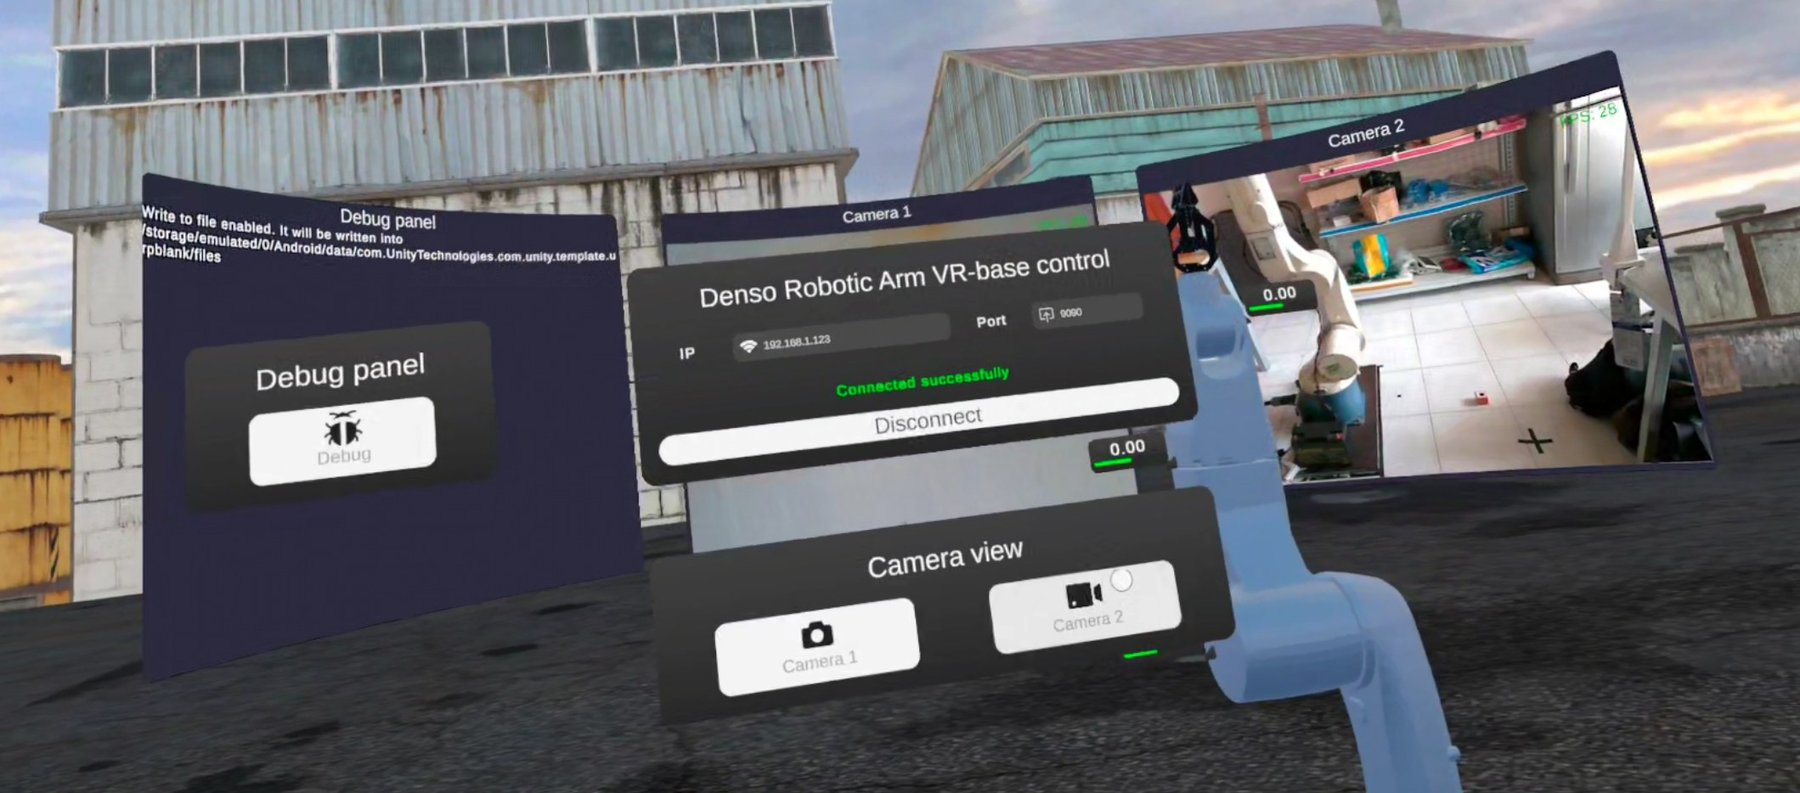
\includegraphics[width=0.8\linewidth]{Images/Implementation/vr_camera.jpg}
    \caption{Hiển thị hai luồng camera trong ứng dụng VR}
    \label{fig:eval-vr-camera}
\end{figure}

\textbf{Điều khiển bằng MoveIt-Servo}

Bảng điều khiển cho phép xoay các trục của cánh tay robot thực tế bằng nút "+" hoặc "-" ở hai bên hàng. Ở giữa hàng, giá trị số cho biết góc của trục tương ứng (đơn vị độ).

\begin{figure}[H]
    \centering
    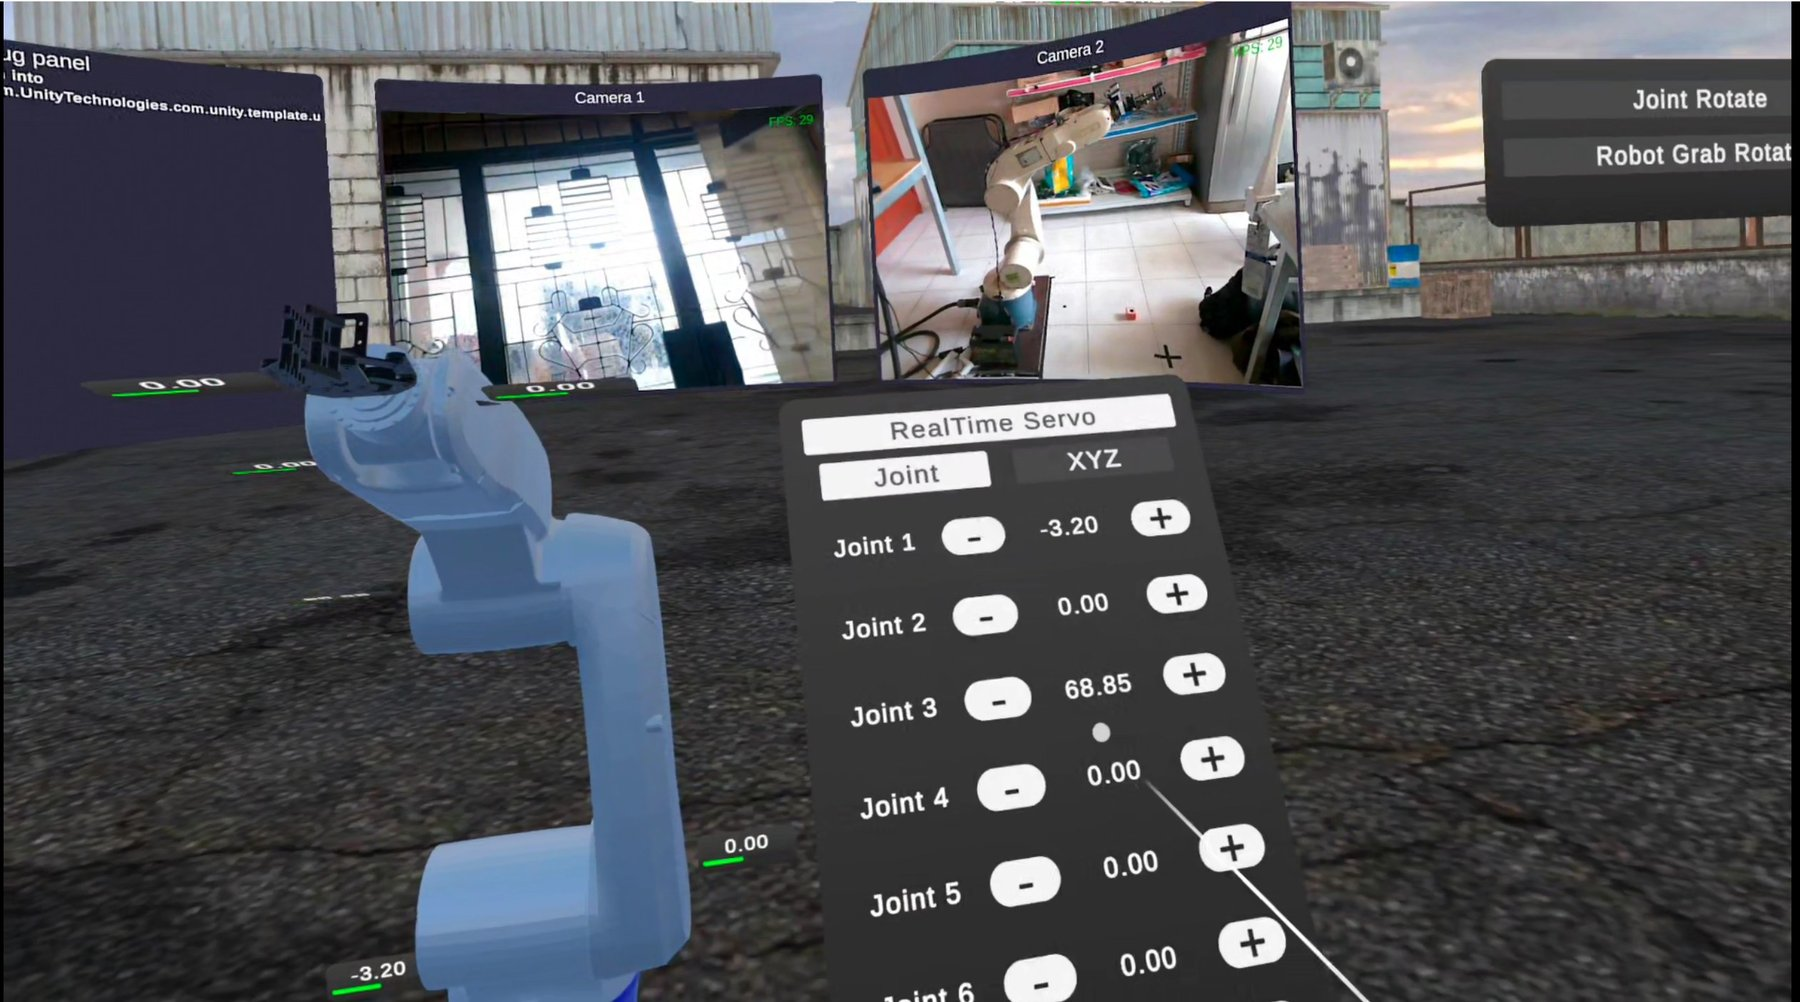
\includegraphics[width=0.8\linewidth]{Images/Implementation/vr_moveit_servo.jpg}
    \caption{Bảng điều khiển MoveIt-Servo trong ứng dụng VR}
    \label{fig:eval-vr-moveit-servo}
\end{figure}

\textbf{Điều khiển tay gắp với GripperCommand Action}

Việc điều khiển tay gắp được tích hợp trên bảng điều khiển MoveIt-Servo do nó cũng điều khiển thiết bị thực tế trực tiếp và đơn giản. Nút nhấn "Close" và "Open" gửi lệnh để đóng hoặc mở phần tay gắp. Trạng thái tay gắp thực tế được phản hồi qua chính mô hình 3D Denso Robot.

\begin{figure}[H]
    \centering
    \begin{subfigure}{0.48\linewidth}
        \centering
        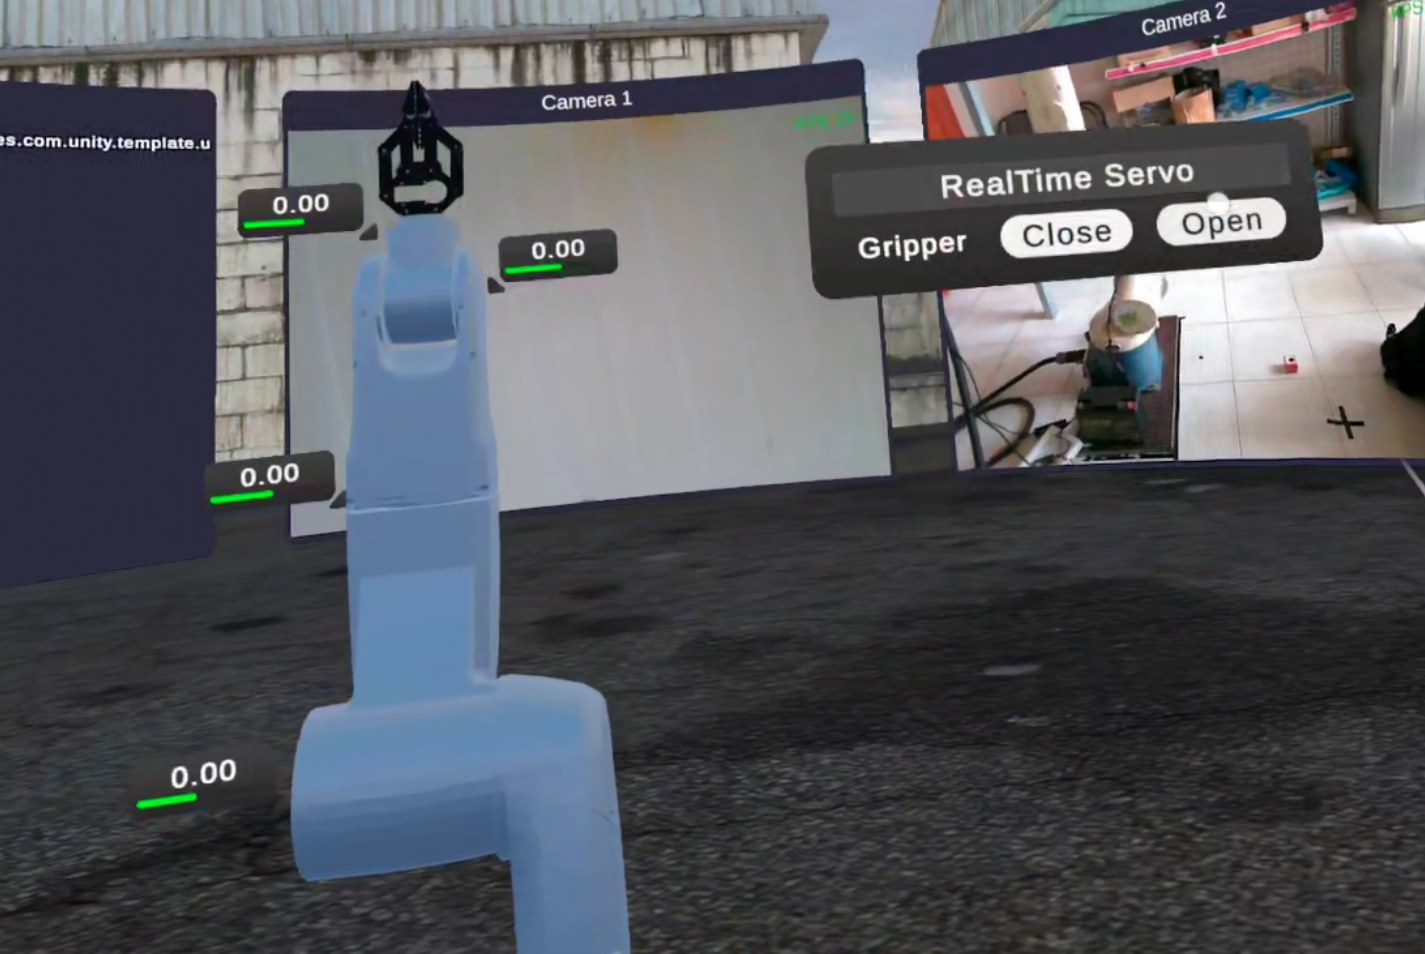
\includegraphics[width=\linewidth]{Images/Implementation/vr_gripper_open.jpg}
        \caption{Tay gắp ở trạng thái đóng}
    \end{subfigure}
    \hfill
    \begin{subfigure}{0.48\linewidth}
        \centering
        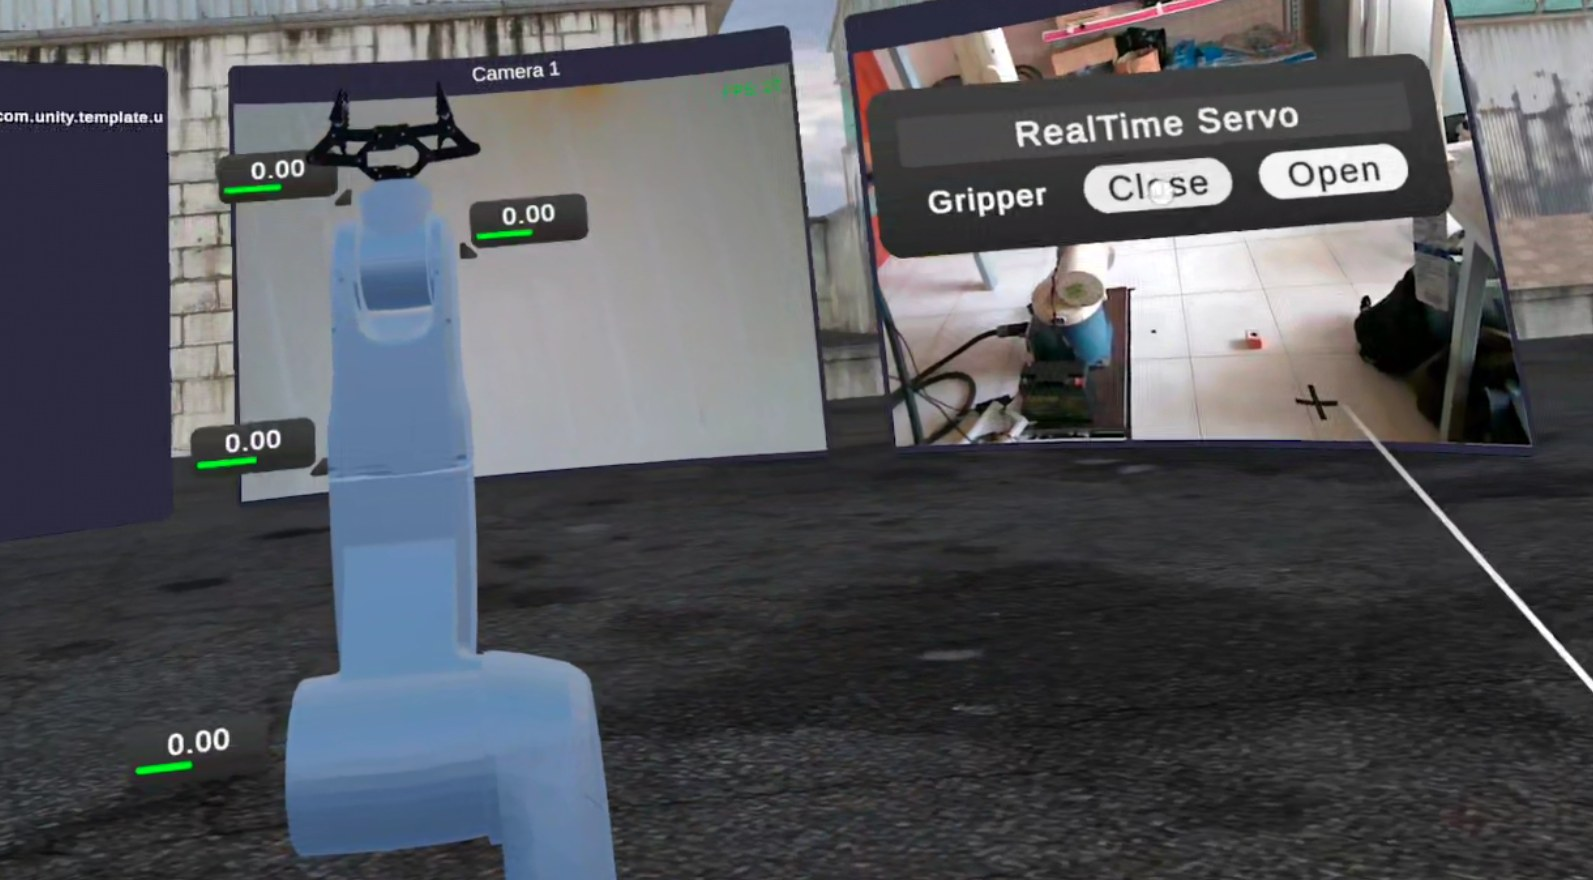
\includegraphics[width=\linewidth]{Images/Implementation/vr_gripper_close.jpg}
        \caption{Tay gắp ở trạng thái mở}
    \end{subfigure}
    \caption{Điều khiển tay gắp bằng GripperCommand Action}
    \label{fig:eval-vr-gripper}
\end{figure}

\textbf{Điều khiển cánh tay robot thông qua các Slider trên bảng điều khiển}

Nhấn vào nút Joint Rotate để chuyển sang bảng điều khiển bằng Slider. Khi này, một robot thứ hai sẽ xuất hiện, và xoay các trục theo giá trị của slider, nhằm cho người dùng biết cánh tay sẽ ở trạng thái như thế nào ở các vị trí tương ứng. Nhấn nút Execute sẽ gửi lệnh tới MoveToPose action server, nhằm điều khiển cánh tay thực tế đạt đến vị trí mong muốn.

\begin{figure}[H]
    \centering
    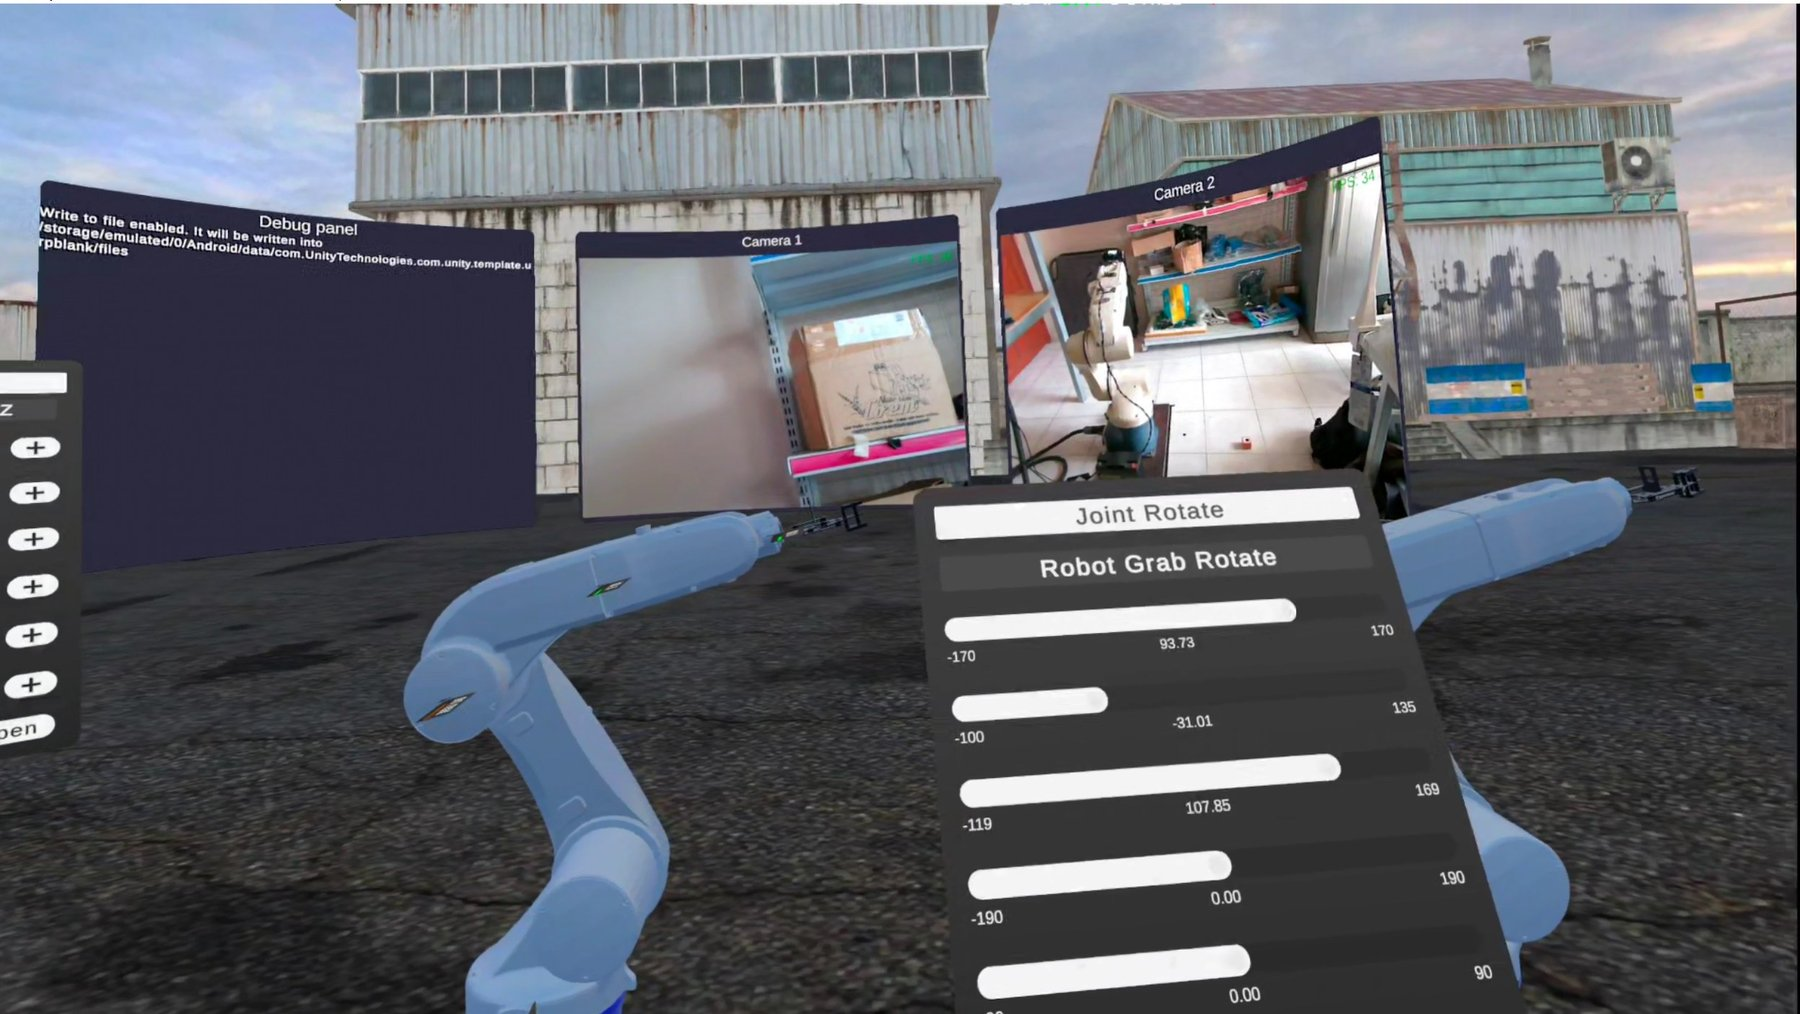
\includegraphics[width=0.8\linewidth]{Images/Implementation/vr_joint_rotate.jpg}
    \caption{Điều khiển cánh tay bằng slider trong ứng dụng VR}
    \label{fig:eval-vr-joint-rotate}
\end{figure}

\textbf{Điều khiển cánh tay robot thông qua tương tác với mô hình tương lai}

Nhấn nút "Robot Grab Rotate" để chuyển sang chế độ điều khiển thông qua việc tương tác (nắm vào kéo) mô hình 3D của cánh tay robot tương lai. Các trục đã được giới hạn để đảm bảo rằng góc kéo không vượt quá ngưỡng hoạt động thực tế của cánh tay robot. Ở phần slider, mỗi trục sẽ thể hiện màu để báo hiệu nếu trục gần đạt đến ngưỡng giới hạn.

Khi đã chỉnh hình dạng của cánh tay robot, nhấn nút Execute sẽ đưa cánh tay thực tế tới vị trí như đã tinh chỉnh.

\begin{figure}[H]
    \centering
    \begin{subfigure}{0.48\linewidth}
        \centering
        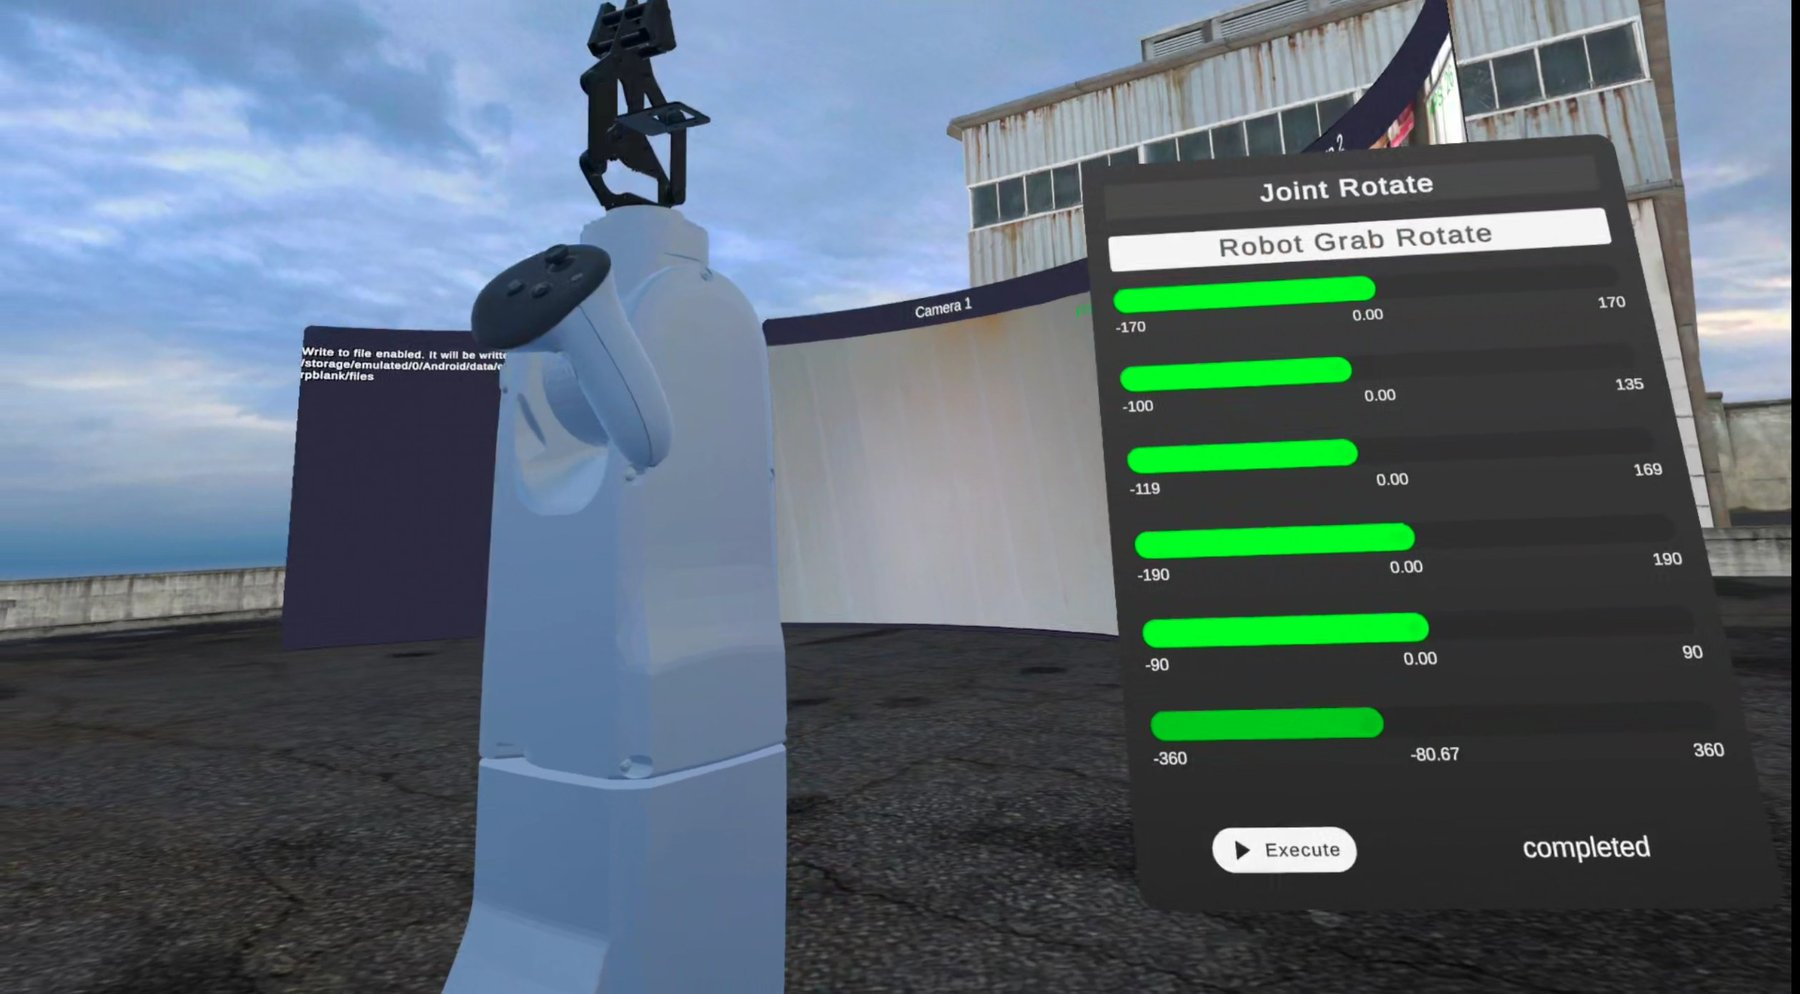
\includegraphics[width=\linewidth]{Images/Implementation/vr_grab_rotate.jpg}
        \caption{Giao diện Robot Grab Rotate}
    \end{subfigure}
    \hfill
    \begin{subfigure}{0.48\linewidth}
        \centering
        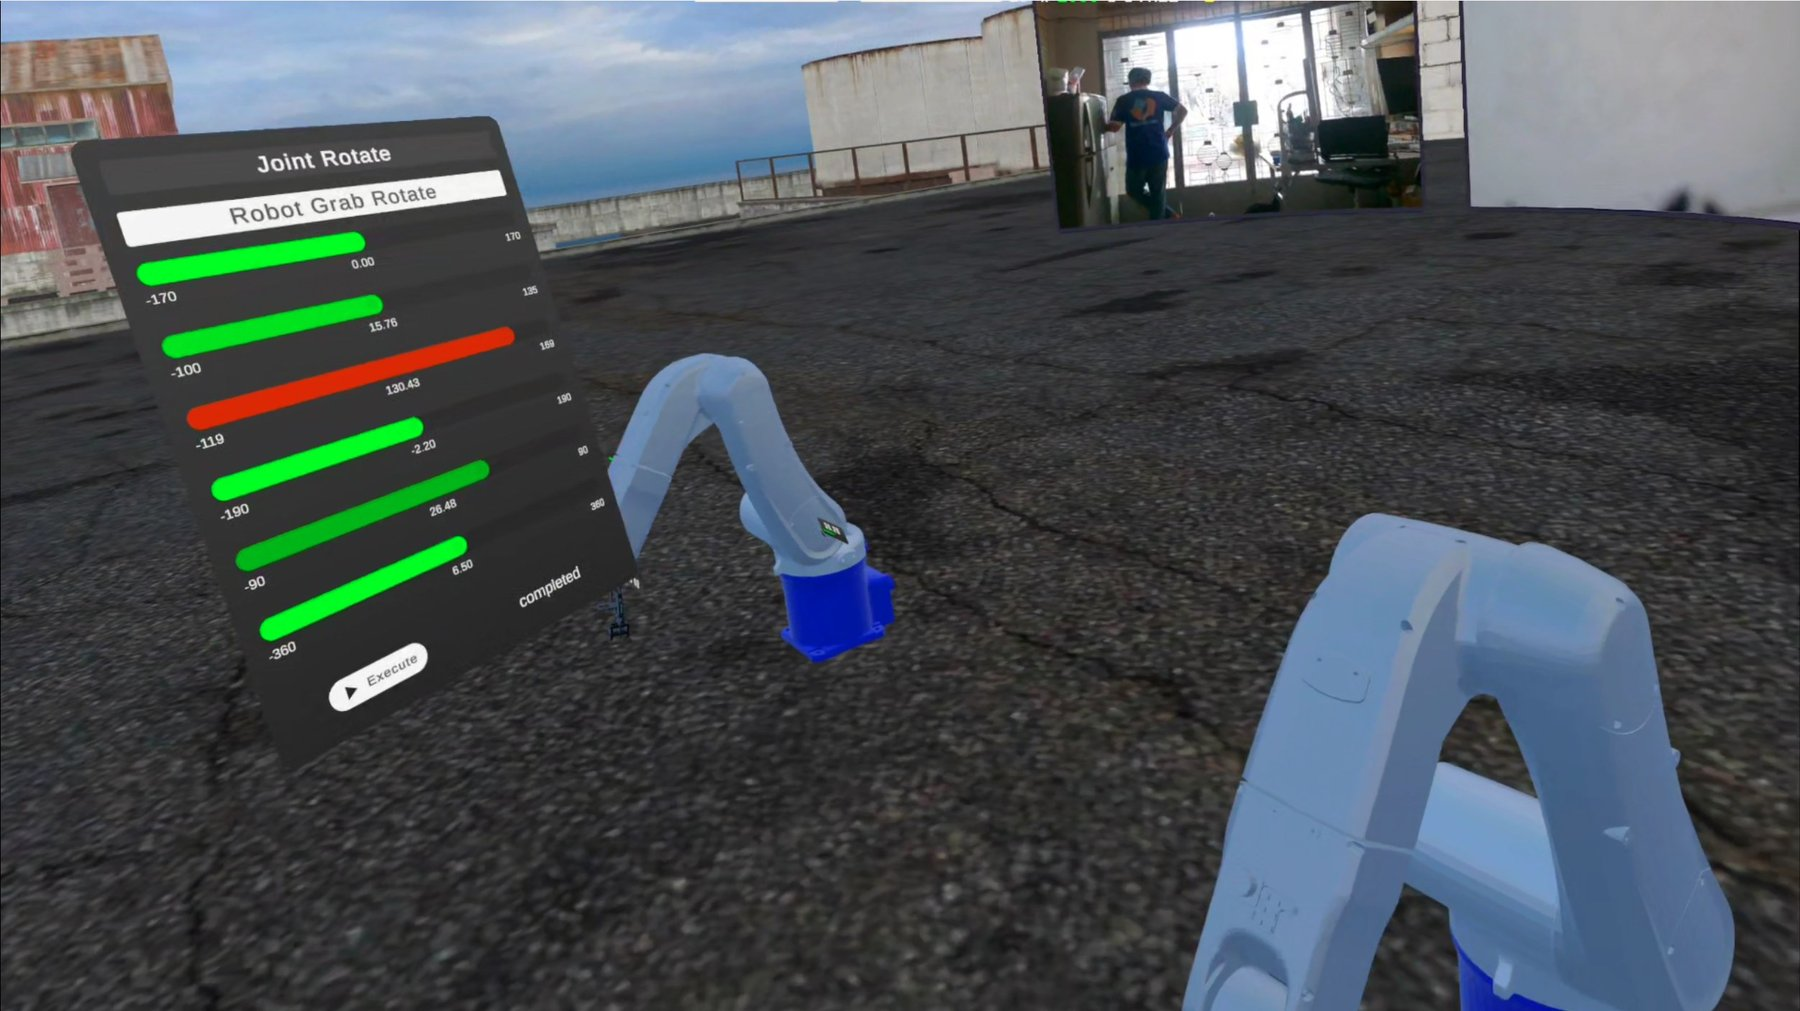
\includegraphics[width=\linewidth]{Images/Implementation/vr_grab_rotate_1.jpg}
        \caption{Thao tác xoay bằng tương tác trực tiếp}
    \end{subfigure}
    \caption{Điều khiển cánh tay bằng tương tác mô hình tương lai}
    \label{fig:eval-vr-grab-rotate}
\end{figure}

\subsubsection{Đánh giá độ trễ truyền nhận thông qua Ros-Sharp giữa ứng dụng và Ros2}

Độ trễ truyền nhận giữa ứng dụng VR và máy PC chạy Ros2 là tiêu chí quan trọng phản ánh mức độ đồng bộ giữa thao tác của người dùng trên kính VR và phản hồi từ hệ thống robot. Để đo đạc chỉ tiêu này, đề tài xây dựng một node Ros2 chuyên dụng (\texttt{topic\_latency\_benchmark}) thực hiện cơ chế ping-pong qua hai topic:

\begin{itemize}
    \item Node Ros2 (PC) publish một gói tin \texttt{std\_msgs/String} lên topic \texttt{/benchmark} mỗi 100\,ms. Payload của gói tin chứa timestamp gửi dưới dạng chuỗi số nanosecond (\texttt{rclcpp::Clock}) để định danh gói.
    \item Ứng dụng VR (Meta Quest~3) subscribe \texttt{/benchmark} thông qua Ros-Sharp/RosBridge WebSocket, sau khi nhận được gói tin, ngay lập tức publish phản hồi lên topic \texttt{/ack} với nội dung payload tương tự.
    \item Khi node Ros2 nhận được \texttt{/ack}, nó tính RTT bằng công thức: 
    
    $\text{RTT} = t_{\text{ack received}} - t_{\text{last benchmark publish}}$, 
    
    với $t$ là thời gian của ROS clock trên cùng máy PC.
\end{itemize}

Phép đo bao gồm toàn bộ đường đi: Ros2 --> ứng dụng VR --> Ros2. Đây là RTT thực tế của vòng giao tiếp điều khiển, chịu một phần ảnh hưởng của độ trễ mạng kết nối.

Để đánh giá khả năng chịu tải mạng, đề tài sử dụng công cụ \textbf{iperf} để mô phỏng băng thông tải cao trên cùng kết nối Wi-Fi. iperf là công cụ đo lường hiệu năng mạng mã nguồn mở, có khả năng tạo ra luồng lưu lượng UDP/TCP liên tục với băng thông tùy chỉnh. Lệnh sử dụng:

\begin{lstlisting}[style=bashstyle]
iperf -c 192.168.2.28 -u -b <x>M -t 0
\end{lstlisting}

Trong đó: \texttt{-c} chỉ định địa chỉ IP của server iperf (máy PC); \texttt{-u} sử dụng giao thức UDP; \texttt{-b <x>M} đặt băng thông mục tiêu \textit{x}\,Mbit/s; \texttt{-t 0} chạy liên tục cho đến khi dừng thủ công. Lệnh này được chạy từ một thiết bị khác trên cùng mạng Wi-Fi, tạo ra lưu lượng nền 100, 150 và 200\,Mbit/s để kiểm tra sự ổn định của kết nối VR--Ros2 khi băng thông bị tải cao. Kết quả đánh giá RTT theo từng điều kiện như sau:

% ── Tự động tạo bởi scripts/analyze_rtt_latency.py ──────────────────────
\begin{figure}[H]
\centering
\begin{tikzpicture}
\begin{axis}[
    ybar,
    width=0.88\linewidth,
    height=6cm,
    bar width=14pt,
    xlabel={Điều kiện tải mạng},
    ylabel={RTT (ms)},
    symbolic x coords={Bình thường, 100 Mbit/s, 150 Mbit/s, 200 Mbit/s},
    xtick=data,
    xticklabel style={font=\small},
    ymin=0, ymax=110,
    ytick={0,20,40,60,80,100},
    ymajorgrids=true,
    major grid style={line width=0.4pt, draw=gray!40},
    legend style={at={(0.98,0.98)}, anchor=north east, font=\small,
                  draw=gray!40, fill=white},
    legend cell align=left,
    axis lines=left,
    enlarge x limits=0.18,
]
% Trung bình (TB)
\addplot[fill=blue!60, draw=blue!80] coordinates {
    (Bình thường, 22.6)
    (100 Mbit/s, 27.4)
    (150 Mbit/s, 38.7)
    (200 Mbit/s, 50.2)
};
\addlegendentry{TB}
% P50 (Trung vị)
\addplot[fill=green!60, draw=green!80!black] coordinates {
    (Bình thường, 19.0)
    (100 Mbit/s, 23.5)
    (150 Mbit/s, 33.3)
    (200 Mbit/s, 52.8)
};
\addlegendentry{P50}
% P95
\addplot[fill=orange!70, draw=orange!90] coordinates {
    (Bình thường, 52.4)
    (100 Mbit/s, 58.3)
    (150 Mbit/s, 82.3)
    (200 Mbit/s, 93.4)
};
\addlegendentry{P95}
% P99
\addplot[fill=red!60, draw=red!80] coordinates {
    (Bình thường, 80.0)
    (100 Mbit/s, 88.0)
    (150 Mbit/s, 95.8)
    (200 Mbit/s, 98.1)
};
\addlegendentry{P99}
\end{axis}
\end{tikzpicture}
\caption{RTT (TB / P50 / P95 / P99) theo điều kiện tải mạng Wi-Fi giữa ứng dụng VR (Meta Quest~3) và Ros2 (PC)}
\label{fig:rtt-bar-chart}
\end{figure}

\begin{table}[H]
\centering
\caption{Thống kê RTT giữa ứng dụng VR và RosBridge WebSocket theo điều kiện tải mạng}
\label{tab:rtt-latency}
\small
\begin{tblr}{
    colspec = {|X[3.2,l]|X[1,c]|X[1.2,c]|X[1.2,c]|X[1.2,c]|X[1.2,c]|X[1.2,c]|X[1.2,c]|},
    hlines,
    row{1} = {font=\bfseries, bg=gray!20},
}
Điều kiện & $N$ & Min (ms) & TB (ms) & Trung vị (ms) & P95 (ms) & P99 (ms) & Max (ms) \\
Bình thường & 1426 & 0{,}8 & 22{,}6 & 19{,}0 & 52{,}4 & 80{,}0 & 97{,}3 \\
Tải cao 100\,Mbit/s & 1001 & 0{,}7 & 27{,}4 & 23{,}5 & 58{,}3 & 88{,}0 & 99{,}4 \\
Tải cao 150\,Mbit/s & 813 & 0{,}4 & 38{,}7 & 33{,}3 & 82{,}3 & 95{,}8 & 99{,}4 \\
Tải cao 200\,Mbit/s & 955 & 0{,}0 & 50{,}2 & 52{,}8 & 93{,}4 & 98{,}1 & 99{,}8 \\
\end{tblr}
\end{table}

Kết quả đo đạc RTT được trình bày tại Bảng~\ref{tab:rtt-latency} và Hình~\ref{fig:rtt-bar-chart}.

\textbf{Điều kiện mạng bình thường.}
Khi không có lưu lượng tải cao ($N = 1426$ mẫu), RTT trung bình đạt
\textbf{22{,}6\,ms} (trung vị 19{,}0\,ms), dao động từ 0{,}8\,ms đến 97{,}3\,ms
với độ lệch chuẩn 13{,}9\,ms.
P95 ở mức \textbf{52{,}4\,ms} và P99 ở mức \textbf{80{,}0\,ms} cho thấy phần lớn
các gói tin được truyền nhận trong vòng 50\,ms -- phù hợp với yêu cầu phản hồi
nhanh của ứng dụng điều khiển thời gian thực qua kính VR.

\textbf{Ảnh hưởng của tải mạng tải cao (iperf UDP).}
Khi áp lưu lượng nền 100\,Mbit/s bằng iperf, RTT trung bình tăng lên
\textbf{27{,}4\,ms} ($+$21{,}4\% so với điều kiện bình thường), P99 tăng lên 88{,}0\,ms.
Ở mức 150\,Mbit/s, RTT trung bình là \textbf{38{,}7\,ms} ($+$71{,}5\%),
và tại 200\,Mbit/s lên tới \textbf{50{,}2\,ms} ($+$122{,}3\%).
RTT tăng theo xu hướng gần tuyến tính với băng thông tải cao, nên để đảm bảo ứng dụng VR có thể giao tiếp hiệu quả với độ trễ thấp, độ lớn của dữ liệu truyền nhận cũng như tính chất của mạng cần được quan tâm.

\textbf{Nhận xét chung.}
Có thể thấy, độ trễ của giao tiếp giữa ứng dụng VR và Ros2 thông qua Ros-sharp vẫn chịu ảnh hưởng của tải mạng, với số liệu cho thấy thời gian RTT tăng dần khi tải mạng tăng cao. Thêm nữa, với việc sử dụng Ros-Sharp, cơ chế giao tiếp giữa ROS2 với kính VR vẫn là giao tiếp thông qua Web Socket (dạng TCP/IP), do đó chịu ảnh hưởng của cơ chế Head-of-line-blocking và nỗ lực truyền dữ liệu tin cậy, cho cả gói tin quan trọng (như /joint\_states) và dữ liệu ảnh lớn (image\_raw), nên sẽ gặp vấn đề nếu lượng dữ liệu truyền đi tăng thêm hoặc mạng bị chập chờn. Để tăng tính hiệu quả của giao tiếp, phương thức giao tiếp sử dụng UDP nên được cân nhắc, có thể thay thế sử dụng Web Socket bằng WebRTC (cho phép tách biệt truyền gói tin dạng UDP cho dữ liệu camera/ cloud sensor, hoặc dữ liệu quan trọng thì sử dụng TCP) với \href{https://docs.phntm.io/bridge/}{Phantom bridge}, và bên phía Unity sẽ phát triển bộ kết nối/ giao tiếp sử dụng WebRTC, trao đổi dữ liệu theo giao thức \href{https://github.com/RobotWebTools/rosbridge_suite/blob/ros2/ROSBRIDGE_PROTOCOL.md#422-default-qos-settings}{RosBridge Protocol V2} để phù hợp theo yêu cầu của Ros2.

Trong đề tài hiện tại, với lợi thế của mạng Wifi cục bộ và việc xây dựng ứng dụng ROS2 sử dụng C++, độ trễ giữa ứng dụng VR và ROS2 rơi vào khoảng 20ms trong điều kiện sử dụng bình thường, qua đó giúp cho việc truyền dữ liệu hình ảnh cũng như đồng bộ trạng thái hoạt động trong 10ms. 

\subsubsection{Đánh giá hiệu năng ứng dụng trong quá trình hoạt động}

Một trong những vấn đề trong việc phát triển ứng dụng VR đó là đảm bảo người dùng có trải nghiệm sử dụng mượt mà, thoải mái mà không gây gánh nặng nhận thức (cognitive pressure). Meta Quest Developer Hub được sử dụng để thu thập chi tiết dữ liệu hoạt động của ứng dụng, gồm nhiều tiêu chí đánh giá khác nhau để xem xét ứng dụng có đang hoạt động ổn định và tối ưu hay không. Bảng phân tích các tiêu chí và nhận xét được thể hiện ở dưới:

Dữ liệu được thu thập qua 1 phiên sử dụng ứng dụng liên tục (tổng cộng
27{,}3\,phút) bằng Meta Quest Developer Hub trên thiết bị Meta Quest 3.
Bảng~\ref{tab:vr-app-metrics} trình bày các tiêu chí hiệu năng chính được ghi nhận
trong suốt quá trình hoạt động.

\begin{table}[H]
\centering
\caption{Tổng hợp hiệu năng ứng dụng VR trên Meta Quest~3 (1 phiên đo, tổng 27{,}3 phút)}
\label{tab:vr-app-metrics}
\small
\begin{tblr}{
    colspec = {|X[4.2,l]|X[1.1,c]|X[1.2,c]|X[1.2,c]|X[1.2,c]|X[1.6,c]|},
    hlines,
    row{1}  = {font=\bfseries, bg=gray!20},
    row{2}  = {bg=gray!10, font=\itshape},
    row{8}  = {bg=gray!10, font=\itshape},
    row{11} = {bg=gray!10, font=\itshape},
    row{14} = {bg=gray!10, font=\itshape},
    row{18} = {bg=gray!10, font=\itshape},
}
Tiêu chí & Đơn vị & TB & Min & Max & Mục tiêu \\
\SetCell[c=6]{l} \textit{Hiệu năng khung hình} \\
FPS trung bình & fps & 72{,}0 & 62 & 73 & $\geq$72 \\
GPU render time / frame & ms & 8{,}60 & 5{,}95 & 11{,}03 & $\leq$13{,}9 \\
ATW GPU time / frame & ms & 1{,}56 & 1{,}12 & 3{,}31 & nhỏ \\
\SetCell[c=6]{l} \textit{Tải CPU / GPU} \\
CPU utilization (tổng 8 nhân) & \% & 52{,}8 & 35 & 69 & $<$80 \\
GPU utilization & \% & 75{,}1 & 55 & 83 & $<$80 \\
Tần số CPU & MHz & 1511 & 1228 & 2361 & -- \\
\SetCell[c=6]{l} \textit{Bộ nhớ} \\
RAM ứng dụng (PSS) & MB & 1010{,}7 & 940 & 1038 & -- \\
GPU memory vật lý & MB & 344{,}2 & 335 & 346 & -- \\
\SetCell[c=6]{l} \textit{Ổn định khung hình (tổng 2 phiên)} \\
Stale frames & frames & \SetCell[c=4]{c} 4307 & & & 0 \\
Skipped frames (ATW miss) & frames & \SetCell[c=4]{c} 0 & & & 0 \\
Shader hitches & lần & \SetCell[c=4]{c} 0 & & & 0 \\
\SetCell[c=6]{l} \textit{Nhiệt độ thiết bị} \\
Nhiệt độ pin & \textdegree{}C & 46{,}3 & 43 & 47 & $<$45 \\
\end{tblr}
\end{table}

\textbf{Khung hình và độ trễ hiển thị.}

\textit{FPS ứng dụng} là số khung hình Unity render được mỗi giây, phản ánh trực tiếp
trải nghiệm mượt mà của người dùng trong môi trường VR. Theo yêu cầu VRC.Quest.Performance.1
của Meta \cite{meta_vrc_performance}, ứng dụng phải duy trì tối thiểu \textbf{60\,fps} liên tục
trong suốt phiên sử dụng; mục tiêu lý tưởng với Meta Quest~3 cấu hình mặc định là bám sát
\textbf{72\,fps} (refresh rate của màn hình). FPS dưới 60 kéo dài gây hiện tượng giật và
tăng nguy cơ say chuyển động (motion sickness). Ứng dụng đạt trung bình \textbf{72{,}0\,fps}
(min 62, max 73), bám sát ngưỡng 72\,fps trong phần lớn phiên sử dụng -- cải thiện đáng kể
so với các phiên đo trước đây.

\textit{GPU render time / frame} (App GPU Time) là thời gian GPU hoàn thành toàn bộ công việc
đồ hoạ cho một frame. Đây là chỉ số then chốt để xác định ứng dụng đang bị bottleneck tại
CPU hay GPU \cite{meta_ovr_best_practices}. Ngân sách frame phụ thuộc vào refresh rate mục
tiêu: tại 72\,Hz là \textbf{13{,}88\,ms}, tại 90\,Hz là 11{,}11\,ms và tại 120\,Hz là
8{,}33\,ms. Nếu App GPU Time vượt ngân sách, ứng dụng bị GPU-bound; ngược lại nếu App GPU
Time thấp nhưng FPS vẫn không đạt, ứng dụng bị CPU-bound. Giá trị đo được \textbf{8{,}60\,ms}
trung bình -- khoảng 62\% ngân sách -- cho thấy pipeline render còn dư headroom; kết hợp với
GPU utilization trung bình 75\%, GPU đang trở thành nút cổ chai chính.

\textit{ATW GPU time / frame} (TimeWarp GPU Time) là thời gian GPU dành riêng cho cơ chế
Asynchronous TimeWarp (ATW) ở tầng compositor của Horizon OS. ATW chạy hoàn toàn độc lập
với ứng dụng: khi ứng dụng không kịp nộp frame đúng hạn, ATW tổng hợp frame trung gian
bằng cách biến đổi frame cũ nhất theo dữ liệu chuyển động đầu mới nhất, duy trì refresh
rate hiển thị. Chỉ số này cần giữ ở mức thấp để không tranh chấp GPU headroom với app;
đỉnh quá cao có thể dẫn tới screen tear \cite{meta_ovr_stats}. Ứng dụng đạt
\textbf{1{,}56\,ms} trung bình (đỉnh 3{,}31\,ms), ở mức an toàn và không cạnh tranh với
App GPU Time.

\textbf{Tải CPU và GPU.}

\textit{CPU utilization} ở đây là tổng mức sử dụng CPU trên cả 8 nhân của SoC Snapdragon
XR2 Gen~2. Cần lưu ý rằng chỉ số này không phân biệt luồng render với các luồng khác
(Ros-Sharp, networking, IK). Mức tải dưới \textbf{80\%} được khuyến nghị để tránh scheduling
pressure ảnh hưởng tới deadline renderer \cite{meta_ovr_stats}; trên 90\% kéo dài sẽ bắt
đầu gây stale frame. Ứng dụng đạt \textbf{52{,}8\%} trung bình với đỉnh \textbf{69\%},
còn dư headroom tốt. CPU không còn là nút cổ chai trong phiên này, nhờ một số cải thiện sau:

\begin{itemize}
    \item \textbf{Tắt mipmaps*}: Trong hàm xử lý ảnh của \textbf{CompressedImageSubscriber}, Texture2D Apply dữ liệu ảnh với tham số \textbf{updateMipmaps = false} và makeNoLongerReadable = false. "Mipmaps" là một khái niệm trong Unity, có vai trò tạo ra nhiều mức độ ảnh (level) cho một đối tượng, và hỗ trợ tự động chọn độ phân giải của đối tượng đó tùy theo khoảng cách với camera. Nếu Camera gần, thì mức độ chi tiết ảnh của đối tượng sẽ giữ chất lượng gốc, nhưng càng ra xa, thì sẽ sử dụng level 1 (nửa độ phân giải), level 2 (1/4 độ phân giải)... Điều này giúp cho game tiết kiệm đáng kể chi phí render hình ảnh đối tượng, giảm tải cho GPU. Tuy nhiên, cơ chế này chỉ phù hợp cho một đối tượng với hình ảnh cố định. Đối với hình ảnh từ camera liên tục thay đổi (30FPS), tính năng này khiến cho Mipmaps bị tính lại liên tục, gây một lượng tải rất lớn cho CPU. Ngoài ra, ảnh camera cũng chỉ được hiển thị trên UI canvas, trên một mặt phẳng, nên việc sử dụng cơ chế Mipmaps là không cần thiết. 
    \item \textbf{Giãn cách lệnh Publish cho MoveIt-Servo control}: Khi nhấn nút xoay robot bằng MoveIt-Servo, hàm được thiết kế ban đầu là gửi lệnh publish liên tục theo framerate. Tuy nhiên, với ~72fps, lệnh publish được gửi với tần số nhanh (13.66ms / 1 lần publish). Điều này vô tình tăng tải xử lý cho CPU để thực hiện publish tới ROS, trong khi đó MoveIt-Servo được cấu hình là chỉ dừng xoay khi lệnh tới trễ hơn 300ms. Do đó, các lớp (Class) Publish vào MoveIt-Servo sẽ chỉ gửi đi mỗi 100ms thay vì mỗi frame, giúp giảm đáng kể tải CPU phải xử lý.
\end{itemize}

\textit{GPU utilization} là mức sử dụng GPU tổng thể của ứng dụng. Ngưỡng
dưới \textbf{80\%} là bình thường; từ 80--90\% bắt đầu có rủi ro scheduling GPU gây frame
drop; 100\% kéo dài nghĩa là GPU-bound hoàn toàn \cite{meta_ovr_stats}. Ứng dụng đạt
\textbf{75{,}1\%} trung bình (đỉnh 83\%), tiệm cận ngưỡng an toàn 80\%. Chỉ số này
nhất quán với App GPU Time ở mức 8{,}60\,ms (62\% ngân sách) và xác nhận GPU hiện là
nút cổ chai chính; đỉnh 83\% cho thấy cần tối ưu hóa draw call và shader để tránh frame drop. Tuy vậy, đây vẫn là một mức tiêu thụ GPU chấp nhận được, và cho ra kết quả hoạt động ứng dụng có FPS trung bình nằm ở mức 72FPS.

\textit{Tần số CPU} phản ánh cơ chế DVFS (Dynamic Voltage and Frequency Scaling) của SoC:
xung tăng tự động khi tải cao và giảm khi nhiệt độ tiệm cận ngưỡng throttle nhiệt. Tần số
dao động từ \textbf{1228\,MHz} đến \textbf{2361\,MHz} trong suốt phiên, cho thấy hệ thống
boost clock khi cần nhưng chưa xảy ra throttle (nếu throttle, tần số sẽ tụt đột ngột
xuống dưới mức nền và kèm theo FPS giảm bất thường).

\textbf{Bộ nhớ.}

\textit{RAM ứng dụng (PSS -- Proportional Set Size)} là dấu chân bộ nhớ RAM thực tế của
tiến trình, trong đó các vùng nhớ chia sẻ với tiến trình khác chỉ được tính theo tỉ lệ sử
dụng. PSS chính xác hơn RSS (Resident Set Size) vì tránh đếm trùng bộ nhớ chia sẻ, đây là
chỉ số chuẩn Android để theo dõi footprint thực \cite{android_memory_overview}. Giá trị
\textbf{1010{,}7\,MB} trung bình (đỉnh 1038\,MB) ổn định, không tăng tuyến tính theo thời gian,
không có dấu hiệu memory leak -- chứng tỏ Unity đang giải phóng Texture2D từ luồng ảnh
camera và các object tạm đúng cách. Mức PSS cao hơn so với báo cáo trước đó là do bật tính năng Development Build (để theo dõi hiệu năng ứng dụng và hỗ trợ Profiling) cùng Immersive Debugging (một tính năng đặc biệt dành cho thiết bị Meta Quest, cho phép hiển thị bảng Debug Log của Unity ngay trong ứng dụng).

\textit{GPU memory vật lý} là phần bộ nhớ đồ hoạ thực tế ứng dụng chiếm dụng cho
texture, framebuffer, mesh buffer và shader. Giá trị \textbf{344{,}2\,MB} trung bình (đỉnh
346\,MB) ổn định, phản ánh asset 3D của cánh tay robot Denso cùng các shader được tải vào
VRAM một lần và giữ xuyên suốt phiên, không có spike lớn do texture streaming bất thường.

\textbf{Ổn định khung hình.}

\textit{Stale frames} là số lần compositor đã sẵn sàng hiển thị frame mới nhưng ứng dụng
chưa nộp frame đúng hạn, khiến compositor phải dùng lại frame cũ và nhờ ATW bù chuyển động.
Khác với skipped frame, stale frame vẫn được hiển thị nhờ ATW nhưng nội dung scene chưa
được cập nhật -- người dùng có thể nhận thấy lag nhỏ giữa chuyển động đầu và phản hồi
hình ảnh \cite{meta_ovr_stats}. \textbf{4307 stale frames} trong 27{,}3 phút
($\approx$2{,}6/giây) -- giảm hơn 75\% so với phiên đo trước (17\,059 stale frames),
phản ánh cải thiện rõ rệt sau khi tối ưu hoá luồng điều khiển. Stale frame còn lại chủ yếu
xuất hiện tại các thời điểm GPU utilization đạt đỉnh 83\%; hướng cải thiện tiếp theo là
tối ưu GPU load để đưa stale frame về gần 0.

\textit{Skipped frames (ATW miss)} là số frame bị compositor bỏ qua hoàn toàn -- tức kể
cả ATW cũng không kịp tổng hợp frame trước deadline scan-out của màn hình. Đây là tình
huống nghiêm trọng nhất: người dùng thấy hình ảnh bị đứng/nhảy cóc, đây là nguyên nhân
hàng đầu gây motion sickness. Mục tiêu cứng của Meta là \textbf{0 skipped frame}
\cite{meta_ovr_stats}. Kết quả đo được \textbf{0 skipped frames} trong toàn phiên
là lý tưởng, xác nhận ATW GPU time (1{,}56\,ms) đủ thấp để compositor luôn hoàn thành
trước deadline dù ứng dụng có bị stale.

\textit{Shader hitches} là số lần Unity phải compile shader lúc runtime (pipeline
compilation stall), gây frame drop đột ngột thường thấy ở lần chạy đầu sau cài đặt khi
shader cache còn trống. Sau khi shader được compile và cache lại, hitches không còn xuất
hiện ở các phiên tiếp theo \cite{meta_ovr_best_practices}. \textbf{0 shader hitches} trong
phiên đo xác nhận shader đã được warm-up đúng cách trước khi thu thập dữ liệu (theo như Meta Quest, để đánh giá chính xác hiệu năng ứng dụng, sẽ cần phải khởi động ứng dụng lần đầu tiên để compile toàn bộ shader, sau đó mới tiến hành đo đạc).

\textbf{Nhiệt độ thiết bị.}

\textit{Nhiệt độ pin} là chỉ báo gián tiếp về nguy cơ thermal throttle của headset. Meta
Quest 3 có ba power state do Horizon OS quản lý \cite{meta_ovr_stats}: \textbf{NORMAL} (hoạt
động bình thường), \textbf{SAVE} (giảm xung CPU/GPU để tản nhiệt, khoảng \textasciitilde45--50\,°C
tuỳ cảm biến), và \textbf{DANGER} (hiển thị cảnh báo quá nhiệt và buộc giảm hiệu năng
nghiêm trọng, khoảng \textasciitilde53\,°C). Khi vào SAVE, FPS và chất lượng render bị
giảm tự động dù ứng dụng không thay đổi. Nhiệt độ pin đo được \textbf{46{,}3\,°C} trung
bình (đỉnh 47\,°C) vượt nhẹ mức 45\,°C Meta khuyến nghị cho trải nghiệm thoải mái nhưng
chưa đạt ngưỡng SAVE hay DANGER. Thiết bị duy trì ổn định ở power state NORMAL trong suốt
phiên 27{,}3 phút;





\chapter{TỔNG KẾT VÀ HƯỚNG PHÁT TRIỂN}
\section{Tổng kết}

Trong giai đoạn 1, nhóm đã hiện thực tương đối yêu cầu đối với việc điều khiển phần cứng: Làm quen với cánh tay robot Denso và cách thức điều khiển thông qua máy RC5, đồng thời xây dựng thành công chương trình điều khiển robot bằng Ros2 kết hợp Ros2-Control và MoveIt bằng ngôn ngữ C++ với thiết kế theo hướng dễ mở rộng, dễ bảo trì và có thể phù hợp với nhiều loại cánh tay robot khác nhau. So với kiến trúc ban đầu gồm 5 thành phần: \textbf{Cánh tay robot Denso VS-6577, máy điều khiển RC5, PC controller, các Camera và kính thực tế ảo (VR)}, nhóm đã làm quen và hiện thực tương đối ba thành phần đầu tiên của hệ thống, và dự tính sẽ tiếp tục phát triển ba thành phần này và hiện thực, tích hợp hai thành phần còn lại để tạo nên một hệ thống điều khiển hoàn chỉnh.

\subsection{Đánh giá hiệu suất của các thành phần}

Với ba thành phần đã hiện thực, nhóm có thực hiện tự đánh giá như sau:

\begin{itemize}
    \item \textbf{Điều khiển cánh tay robot Denso VS-6577 với RC5}: Về cơ bản, nhóm đã làm quen và hiểu được cách để vận hành cánh tay robot theo vị trí từng trục cùng với việc thu thập dữ liệu các trục xoay.
    
    Tuy nhiên nhóm vẫn chưa vận dụng được các tính năng điều khiển chi tiết mà nhà sản xuất cung cấp, các hàm chuyển động robot chưa được tìm hiểu và sử dụng đa dạng. Nhóm cũng chưa điều khiển được vận tốc quay và vấn đề gia tốc khi di chuyển từng bước một cách linh hoạt, mà hiện phải chọn một tốc độ chậm cố định cho mọi trục trên RC5, dẫn tới thuật toán điều khiển robot ROS2 cũng phải điều chỉnh để chậm theo thiết bị và đảm bảo thao tác nằm trong khoảng thời gian cho phép.

    \item \textbf{Giao tiếp UART giữa RC5 và PC Controller}: Nhóm đã tìm được phương pháp giao tiếp phù hợp và hợp lý giữa máy điều khiển RC5 (với thiết kế tương đối cũ) và PC Controller thông qua cổng RS232, đồng thời hiểu được cách dữ liệu được xử lý thế nào trong RC5 và sử dụng các lệnh phù hợp. 

    Tuy vậy, với baud rate 19200, tốc độ giao tiếp này vẫn có thể xem là chưa đủ nhanh cho ứng dụng thời gian thực, và nhóm thường gặp vấn đề máy RC5 sẽ bị lỗi "tag error" khi tăng tốc độ truyền lệnh của PC Controller nhanh hơn và máy RC5 chưa thể xử lý kịp. Ngoài ra, việc nhận lệnh điều khiển đang phải chờ cho cánh tay hoạt động xong mới nhận, gây ra khả năng mất dữ liệu khi robot đang thực hiện thao tác quay.

    \item \textbf{Xây dựng hệ thống điều khiển thời gian thực ROS2 trên PC Controller}: Đây là phần nhóm dành nhiều thời gian hiện thực và tìm hiểu, với chú trọng tích hợp được giữa mô hình 3D của cánh tay robot Denso VS-5677, thiết kế dự án tích hợp giữa ROS2, Ros2-Control và MoveIt tuân thủ theo kiến trúc được đề xuất bởi Ros2-Control, hơn nữa còn sử dụng ngôn ngữ C++ thay vì Python để tăng khả năng xử lý đa luồng, từ đó đảm bảo yêu cầu điều khiển thời gian thực đã đề ra ban đầu. Nhóm cũng cố gắng thiết kế chương trình có tính mở rộng và tinh chỉnh cao, tận dụng các file cấu hình bên ngoài giúp việc thay đổi hoạt động điều khiển trở nên dễ dàng hơn, và thậm chí phần Hardware Interface có thể được tận dụng lại cho các mô hình cánh tay robot khác.

    Nhưng điểm yếu của hiện thực hiện tại, vẫn là chưa thể điều khiển robot trong thời gian thực, tốc độ của chu kì read-update-write vẫn còn thấp (chỉ 2Hz) do giới hạn về cách thức điều khiển phần cứng cũng như tốc độ truyền lệnh. Dự án cũng chưa tận dụng được các công cụ mô phỏng như Gazebo, do đó có tính phụ thuộc vào phần cứng và làm chậm khả năng phát triển các tính năng khác. Việc điều khiển bằng tốc độ cũng chưa được ứng dụng triệt để, dù có chuẩn bị sẵn do thiếu phương pháp điều khiển tốc độ của cánh tay robot. 
\end{itemize}

%phải lên 1 kiến trúc tổng quát, rồi module nào dc hiệu suất ra sao, tương lai làm cái nào để hoàn thiện luận văn, tối ưu chỗ nào, cải tiến chỗ nào, cố gắng làm rõ ra

\section{Hướng phát triển}

Dựa vào kết quả hiện tại và những hạn chế nhận biết được, nhóm sẽ tiếp tục phát triển, hoàn thiện hệ thống điều khiển cánh tay robot thông qua kính VR, qua việc tiếp tục cải thiện những điểm hạn chế từ kết quả hiện tại và hiện thực những thành phần còn thiếu trong hệ thống.

\subsection{Những điểm cần cải tiến}

Nhóm sẽ tiến hành cải tiến, chủ yếu là về phía điều khiển giữa cánh tay VS-5677 và RC5, giữa RC5 và PC Controller, qua đó đáp ứng khả năng điều khiển phần cứng thời gian thực, cụ thể:

\begin{itemize}
    \item Lắp thêm phần đế hoặc tìm cách cố định cánh tay robot trên mặt phẳng. Hiện tại, nhóm chỉ có thể điều khiển cánh tay ở tốc độ thấp do cánh tay thiếu phần đế vững chắc, khi quay quá nhanh sẽ khiến cánh tay bị lật/ ngã.
    \item Tối ưu cách thức điều khiển giữa khối RC5 và cánh tay robot Denso VS-6577, thêm nhiều kiểu lệnh điều khiển mới và có cơ chế phản hồi sau mỗi lệnh điều khiển. Thêm khả năng điều khiển vận tốc linh hoạt khi di chuyển, và nghiên cứu khả năng tùy chỉnh gia tốc để chuyển động. 
    \item Làm quen và vận dụng trình mô phỏng Gazebo với hiện thực ROS2 hiện tại để tránh phụ thuộc nhiều vào phần cứng
    \item Tối ưu tốc độ truyền và xử lý dữ liệu UART trên cả RC5 và PC controller để cho phép tần suất chạy Ros2-Control cao hơn.
    \item Tạo cơ chế điều khiển vận tốc thay vì chỉ tốc độ cho cánh tay hiện tại thông qua định dạng lệnh mới và code xử lý mới ở RC5
\end{itemize}

\subsection{Những thành phần cần hiện thực}

So với hệ thống đã đề xuất, nhóm vẫn còn thiếu các thành phần ở lớp ứng dụng - trên cả PC controller và ứng dụng trên kính thực tế ảo VR. Hướng hiện thực của nhóm trong luận văn sẽ tập trung vào:

\begin{enumerate}
    \item Xây dựng module điều khiển ROS2 cao hơn Moveit, cung cấp những topic cần thiết cho điều khiển VR
    \item Tìm hiểu và hiện thực cơ chế truyền dữ liệu và hình ảnh, video hiệu quả, độ trễ thấp thông qua ROS2. Cơ chế này cần hỗ trợ ít nhất 2 luồng dữ liệu camera khác nhau để đảm bảo tính phản ảnh thế giới thực tốt trong ứng dụng VR
    \item Xây dựng ứng dụng VR có khả năng điều khiển cánh tay robot từ xa và cập nhật trạng thái với độ trễ thấp.
    \item Xây dựng khả năng tương tác linh hoạt với mô hình cánh tay Robot trong môi trường VR.
\end{enumerate}

\nocite{*}

\printbibliography[
heading=bibintoc,
title=Tài liệu tham khảo,
]

\newpage
\begin{center}
    \bf{THÔNG TIN HỌC VIÊN}
\end{center}
Danh sách tác giả Đồ Án:
\begin{enumerate}
    \item \textbf{Trần Ngọc Cát} - ID: 2370415
    \begin{itemize}
        \item Số điện thoại: (+84)975.598.049
        \item Email: tncat.sdh232@hcmut.edu.vn
    \end{itemize}
\end{enumerate}


\end{document}
%%21:16:49 1/9/2012Last Modification of contents